\documentclass[10pt]{article}
\usepackage{tmlr}
\usepackage{amsmath,amssymb,amsthm,mathtools,booktabs,microtype,enumitem,longtable,array}
\usepackage{graphicx}
\usepackage{placeins}
\usepackage{hyperref}
\usepackage{url}
\hypersetup{hidelinks,
 pdftitle={Kernel Affine Hull Representations for Time-Series Forecasting: Distinctness, Stability, and Predictive Limits},
 pdfauthor={Anonymous authors},
 pdfsubject={Reconstruction representations, bounded residual forecasting, and matched empirical evaluation}}
\newtheorem{proposition}{Proposition}
\allowdisplaybreaks
\newcommand{\R}{\mathbb{R}}
\newcommand{\E}{\mathbb{E}}
\newcommand{\Var}{\operatorname{Var}}
\newcommand{\MSE}{\operatorname{MSE}}
\newcommand{\K}{\mathrm{K}}
\newcommand{\A}{\mathrm{A}}
\newcommand{\clip}{\operatorname{clip}}
% Generated from archived records; descriptive ratios have no ratio intervals.
\newcommand{\ConfirmationReplicates}{24}
\newcommand{\StageOneFamilySize}{29}
\newcommand{\CapacityFamilySize}{12}
\newcommand{\StageOneCriticalValue}{3.545808}
\newcommand{\CapacityCriticalValue}{3.180663}
\newcommand{\FlatWithinAffineMSE}{1.002694}
\newcommand{\FlatWithinKAHMMSE}{0.024668}
\newcommand{\FlatWithinNativeAffineMSE}{0.004641}
\newcommand{\FlatWithinRawMSE}{0.003330}
\newcommand{\FlatWithinGeometryGain}{0.978026}
\newcommand{\FlatAlignmentInteraction}{-0.978039}
\newcommand{\CurvedAlignmentInteraction}{-0.009564}
\newcommand{\VDPPhiRidgeMSE}{0.111108}
\newcommand{\VDPKAHMLocalRidgeMSE}{0.014475}
\newcommand{\VDPAffineLocalRidgeMSE}{0.011582}
\newcommand{\AirfoilRawRidgeMSE}{19.4726}
\newcommand{\AirfoilRawRBFMSE}{15.6898}
\newcommand{\AirfoilKAHMLocalRBFMSE}{20.9313}
\newcommand{\LocalPracticalBenefitCount}{8}
\newcommand{\CapacityPracticalBenefitCount}{4}
\newcommand{\VDPRawNarrowMSE}{0.002858644}
\newcommand{\VDPAffineNarrowMSE}{0.001376729}
\newcommand{\VDPKAHMNarrowMSE}{0.001026627}
\newcommand{\VDPRawNarrowRelativeGain}{64.1}
\newcommand{\VDPAffineNarrowRelativeGain}{25.4}
\newcommand{\VDPRawWideMSE}{0.001654150}
\newcommand{\VDPAffineWideMSE}{0.001078003}
\newcommand{\VDPKAHMWideMSE}{0.000871969}
\newcommand{\VDPRawWideRelativeGain}{47.3}
\newcommand{\VDPAffineWideRelativeGain}{19.1}
\newcommand{\NumericalOriginalZeroCount}{99,762}
\newcommand{\NumericalQueryClusterCount}{2,236,416}

% Generated from the unchanged confirmation method/policy reports.
\newcommand{\NaturalRawLoss}{0.8075}
\newcommand{\NaturalKAHMLoss}{0.8419}
\newcommand{\NaturalRidgeLoss}{0.7798}
\newcommand{\NaturalRawCost}{0.1688}
\newcommand{\NaturalKAHMCost}{0.3874}
\newcommand{\NaturalRidgeCost}{0.1880}
\newcommand{\NaturalErrorIncrease}{4.26}
\newcommand{\NaturalCostRatio}{2.30}
\newcommand{\NaturalProbeLoss}{0.807085}
\newcommand{\NaturalProbeCost}{0.3309}
\newcommand{\NaturalProbeCostRatio}{1.96}
\newcommand{\NaturalProbeGainPercent}{0.054}

% Generated by scaling_sensitivity/report.py from analysis/summary.json.
\newcommand{\ScalingNaturalKahmStandardLoss}{0.8419}
\newcommand{\ScalingNaturalKahmMinmaxLoss}{0.8422}
\newcommand{\ScalingNaturalRawLoss}{0.8075}
\newcommand{\ScalingNaturalRidgeLoss}{0.7798}
\newcommand{\ScalingNaturalKahmChangePercent}{0.03}
\newcommand{\ScalingNaturalKahmReductionPercent}{-0.03}
\newcommand{\ScalingNaturalKahmVsRawPercent}{4.29}
\newcommand{\ScalingNaturalKahmVsRidgePercent}{8.00}
\newcommand{\ScalingNaturalKahmStandardTime}{0.3804}
\newcommand{\ScalingNaturalKahmMinmaxTime}{0.5561}
\newcommand{\ScalingNaturalRawTime}{0.1762}
\newcommand{\ScalingNaturalRidgeTime}{0.1863}
\newcommand{\ScalingNaturalKahmCostRatioRaw}{3.16}
\newcommand{\ScalingNaturalKahmCostRatioStandard}{1.46}
\newcommand{\ScalingNaturalFamiliesImproved}{2}
\newcommand{\ScalingDevelopmentKahmStandardLoss}{2.1768}
\newcommand{\ScalingDevelopmentKahmMinmaxLoss}{2.3444}
\newcommand{\ScalingDevelopmentKahmChangePercent}{7.70}

% Generated from the fully attempted, failure-aware audited utility run.
% Archive method means without FullRoster in their name are POST-HOC common-support diagnostics.
\newcommand{\UtilityTaskCount}{168}
\newcommand{\UtilitySyntheticTasks}{144}
\newcommand{\UtilityArchiveTasks}{24}
\newcommand{\UtilityWarnings}{8}
\newcommand{\UtilityArchiveCompleteTasks}{22}
\newcommand{\UtilitySuccessfulForecasts}{1336}
\newcommand{\UtilityFailedFits}{8}
\newcommand{\UtilityFailedPolicies}{4}
\newcommand{\UtilityRawLoss}{9.1730}
\newcommand{\UtilityRawCost}{0.0037}
\newcommand{\UtilityRawCostRatio}{1.00}
\newcommand{\UtilityRawGainPercent}{0.00}
\newcommand{\UtilityRawFullRosterLoss}{9.6633}
\newcommand{\UtilityRidgeLoss}{0.8466}
\newcommand{\UtilityRidgeCost}{0.0015}
\newcommand{\UtilityRidgeCostRatio}{0.41}
\newcommand{\UtilityRidgeGainPercent}{90.77}
\newcommand{\UtilityRidgeFullRosterLoss}{1.2848}
\newcommand{\UtilityConcatLoss}{1.2111}
\newcommand{\UtilityConcatCost}{0.0691}
\newcommand{\UtilityConcatCostRatio}{18.44}
\newcommand{\UtilityConcatGainPercent}{86.80}
\newcommand{\UtilityKAHMLoss}{9.1443}
\newcommand{\UtilityKAHMCost}{0.0498}
\newcommand{\UtilityKAHMCostRatio}{13.29}
\newcommand{\UtilityKAHMGainPercent}{0.31}
\newcommand{\UtilityAffineLoss}{9.3312}
\newcommand{\UtilityAffineCost}{0.0369}
\newcommand{\UtilityAffineCostRatio}{9.83}
\newcommand{\UtilityAffineGainPercent}{-1.72}
\newcommand{\UtilityLocalityLoss}{9.5624}
\newcommand{\UtilityLocalityCost}{0.0379}
\newcommand{\UtilityLocalityCostRatio}{10.10}
\newcommand{\UtilityLocalityGainPercent}{-4.24}
\newcommand{\UtilityNaiveLoss}{1.2062}
\newcommand{\UtilityNaiveCost}{0.0012}
\newcommand{\UtilityNaiveCostRatio}{0.32}
\newcommand{\UtilityNaiveGainPercent}{86.85}
\newcommand{\UtilityNaiveFullRosterLoss}{1.5720}
\newcommand{\UtilityHGBLoss}{10.3174}
\newcommand{\UtilityHGBCost}{0.6380}
\newcommand{\UtilityHGBCostRatio}{170.20}
\newcommand{\UtilityHGBGainPercent}{-12.48}
\newcommand{\UtilityHGBFullRosterLoss}{10.7552}
\newcommand{\UtilityPolicyLoss}{9.2460}
\newcommand{\UtilityPolicyCost}{0.0467}
\newcommand{\UtilityPolicyCostRatio}{12.45}
\newcommand{\UtilityPolicyGainPercent}{-0.80}
\newcommand{\UtilityGeometryPolicyLoss}{9.2624}
\newcommand{\UtilityGeometryPolicyCost}{0.0869}
\newcommand{\UtilityGeometryPolicyCostRatio}{23.17}
\newcommand{\UtilityGeometryPolicyGainPercent}{-0.97}
\newcommand{\UtilityRawPositiveContrasts}{5}
\newcommand{\UtilityRawNegativeContrasts}{0}
\newcommand{\UtilityRawUnresolvedContrasts}{7}
\newcommand{\UtilityConcatPositiveContrasts}{6}
\newcommand{\UtilityConcatNegativeContrasts}{4}
\newcommand{\UtilityConcatUnresolvedContrasts}{2}
\newcommand{\UtilityKAHMAdoptions}{7}
\newcommand{\UtilityGeometryAdoptions}{12}
\newcommand{\UtilityArchiveKAHMNonzero}{9}
\newcommand{\UtilitySyntheticKAHMNonzero}{134}

% Generated target-geometry numbers; change is signed, negative favorable.
\newcommand{\TGTaskCount}{48}
\newcommand{\TGCompletedTaskCount}{48}
\newcommand{\TGForecastCount}{768}
\newcommand{\TGMethodCount}{16}
\newcommand{\TGFallbackCount}{0}
\newcommand{\TGPrimaryPositive}{3}
\newcommand{\TGPrimaryNegative}{5}
\newcommand{\TGPrimaryUnresolved}{10}
\newcommand{\TGNaturalLearnedMSE}{1.2721}
\newcommand{\TGNaturalRidgeMSE}{1.3005}
\newcommand{\TGNaturalChangePercent}{-2.18}
\newcommand{\TGNaturalCostRatio}{124.9}

% Generated from the preserved direct-reconstruction summary; no manual numerical edits.
\newcommand{\DirectPlannedTasks}{46}
\newcommand{\DirectAvailableTasks}{43}
\newcommand{\DirectAvailableOutputs}{731}
\newcommand{\DirectPlannedOutputs}{782}
\newcommand{\DirectUnavailableTasks}{3}
\newcommand{\DirectNaturalAvailableCollections}{3}
\newcommand{\DirectNaturalAvailableSeries}{7}
\newcommand{\DirectPrimaryPositive}{2}
\newcommand{\DirectPrimaryNegative}{6}
\newcommand{\DirectPrimaryUnresolved}{10}
\newcommand{\DirectOptimizations}{3096}
\newcommand{\DirectObjectiveEvaluations}{406832}
\newcommand{\DirectFallbackEvents}{0}

% Complete saved-result macros; generated without fitting models.
\providecommand{\RMTaskCount}{192}
\providecommand{\RMRepeatCount}{24}
\providecommand{\RMMethodCount}{10}
\providecommand{\RMRecordCount}{1{,}920}
\providecommand{\RMTargetCells}{958{,}464}
\providecommand{\RMUsefulPassCount}{1}
\providecommand{\RMContrastPassCount}{2}
\providecommand{\RMKNonlinearNMSE}{0.02993}
\providecommand{\RMKLinearNMSE}{0.89810}
\providecommand{\RMMaxErrorRatio}{1.553}
\providecommand{\RMFeatureViolations}{0}
\providecommand{\RMCoefficientViolations}{0}
\providecommand{\RMCorrectionViolations}{0}
\providecommand{\RMStabilityFailures}{0}
\providecommand{\RMKActiveNonlinear}{432}
\providecommand{\RMKActiveLinear}{54}
\providecommand{\RMKFallbackD}{0}
\providecommand{\RMRFallbackD}{0}
\providecommand{\RMKFallbackABC}{0}
\providecommand{\RMPeakProcessMiB}{173.6}
\providecommand{\RMFreezeShort}{6d666b0fa3d8}
\providecommand{\RMKFitSeconds}{0.0833}
\providecommand{\RMRFitSeconds}{0.0658}
\providecommand{\RMRawRBFFitSeconds}{0.0135}
\providecommand{\RMKPredictionMilliseconds}{29.245}
\providecommand{\RMRPredictionMilliseconds}{25.758}
\providecommand{\RMKStateKiB}{118.81}
\providecommand{\RMKvsCommonGain}{12.58}
\providecommand{\RMKvsCommonLower}{0.00295}
\providecommand{\RMKvsRBFDepartureGain}{1.17}
\providecommand{\RMKvsRBFDepartureLower}{-0.00079}
\providecommand{\RMKvsRawRBFGain}{3.92}
\providecommand{\RMKvsRawRBFLower}{\ensuremath{-8.286\times10^{-5}}}
\providecommand{\RMKvsBoostingGain}{-1.77}
\providecommand{\RMKvsBoostingLower}{-0.00194}
\providecommand{\RMKvsPolicyGain}{-6.04}
\providecommand{\RMKvsPolicyLower}{-0.00299}
\providecommand{\RMLinearLower}{0.04161}
\providecommand{\RMLinearNIPassText}{passes}
\providecommand{\RMDecisionText}{stop this forecasting-performance branch}


\title{Kernel Affine Hull Representations\\
for Time-Series Forecasting:\\
Distinctness, Stability, and Predictive Limits}
\author{Anonymous authors}
\begin{document}
\maketitle
\begin{abstract}
Kernel Affine Hull Machines (KAHMs) construct nonlinear reconstructions
from local reference observations. We study when these reconstructions
provide useful features for a finite-dimensional time-series forecasting
decoder. We show that direct transfer of normalized reconstruction weights
to reference targets is a ratio of kernel-ridge predictions. We identify
conditions under which KAHM and matched radial-basis-function (RBF)
reconstructions generate the same augmented feature span when common
affine features are retained, and construct an irregular
reference set for which their spans differ. A bounded feature transform
and a ridge residual decoder also yield a uniform bound on the magnitude
of the forecast correction. These algebraic properties are distinct from
predictive accuracy. In a prospectively specified experiment, we compare
ten procedures on 192 task suites comprising three nonlinear simulation
laws, a linear control, two observation-noise levels, and 24 independent
repetitions. The bounded KAHM reconstruction departure reduces aggregate
nonlinear normalized mean squared error by \RMKvsCommonGain\% relative
to the shared local-coordinate basis. Its gains over matched RBF
reconstruction and raw-input RBF forecasting are
\RMKvsRBFDepartureGain\% and \RMKvsRawRBFGain\%, respectively; neither
comparison establishes the prespecified 3\% improvement margin under
simultaneous inference. Boosted trees and a validation-selected non-KAHM
procedure attain lower aggregate error. The correction bounds and the
linear-control noninferiority criterion are satisfied. Complementary
controlled, natural-data, and adaptive experiments further delimit the
conditions under which these representations help. The evidence shows
that reconstruction can contribute useful forecasting features, while
neither a distinct feature span nor a bounded correction establishes a
practical advantage specific to KAHM.
\end{abstract}

\section{Introduction}\label{sec:introduction}
A representation is useful for forecasting when the fitted decoder can
extract information relevant to future observations from it. Kernel Affine
Hull Machines (KAHMs) construct nonlinear reconstruction maps from local
reference observations \citep{Kumar2024KAHM}. Such a map can reconstruct
an observed history accurately without providing a useful code for its
future. For example, a reconstruction residual that vanishes along an
affine line loses position along that line, even when the forecasting
target varies with position. More generally, deterministic features cannot
add information to the history from which they are computed, but they can
make different functions available to a restricted, regularized decoder.

This distinction motivates three questions. First, does a KAHM
reconstruction provide functions that a simpler matched representation
cannot express? Second, can the magnitude of the forecast correction
built from those functions be controlled? Third, does the fitted procedure
improve prediction at the available sample size and computational budget?
The answers require different evidence. A difference between function
spans is an algebraic property. A correction bound concerns the magnitude
of a fitted prediction component. Predictive usefulness depends on the
target, the data distribution, regularization, and model selection.

We study these questions using \emph{reconstruction departures}: the
difference between a nonlinear local reconstruction and its affine
projection, multiplied by a locality weight. The decoder also receives
the locality weights and weighted principal coordinates. This common
feature block preserves local position and is identical across the KAHM
and radial-basis-function (RBF) reconstruction procedures. Replacing the
nonlinear reconstruction with the affine projection makes the departure
zero. The resulting common-feature procedure therefore isolates the
contribution of the additional reconstruction features. A positive-kernel
RBF reconstruction, using the same references, kernel, and locality
weights, provides a more closely matched comparison.

Our analysis first identifies cases in which the apparent additional
structure is redundant. Applying normalized KAHM reconstruction weights
to reference targets gives exactly a ratio of two kernel-ridge predictions:
one fitted to the targets and one fitted to a constant response.
Symmetric reference sets can also produce the same augmented raw feature
span for KAHM and RBF reconstruction. In contrast, an explicit irregular
three-reference construction yields a KAHM departure outside the span of
the corresponding affine and RBF features. This establishes that the
reconstruction can change the available basis under stated conditions.
It does not establish a general advantage over kernel regression.
Moreover, isotropic ridge regularization and nonlinear feature
normalization depend on the feature parameterization. The empirical
comparison therefore concerns the complete fitted procedures, even when
two unregularized feature spans coincide.

The stability analysis addresses a separate difficulty. In an adaptive
experiment, a numerical solver correction removed computational exceptions
but did not eliminate extreme forecasts. Recomputing an examined state
with a fresh solve reproduced the extreme correction, showing that a
correct linear solve alone does not control extrapolation through the
features. We consequently study a fixed-geometry construction that
normalizes and bounds each feature block before fitting a ridge residual
decoder. We prove a uniform correction-magnitude bound that includes the
free intercept and specifies the scaling of the ridge penalty. The bound
does not control the raw baseline or guarantee small forecast error.

The principal forecasting experiment compares ten procedures across three
nonlinear simulation laws and a linear Gaussian autoregressive control,
with two levels of additional observation noise. Twenty-four independent
repetitions yield 192 task suites. Four episode sets have separate roles:
fitting, hyperparameter selection, correction calibration, and final
evaluation. The protocol, source code, analysis, and prepared inputs were
recorded locally before the final forecasts were computed. This prospective
record was not a public preregistration. Five comparisons test whether the
KAHM procedure improves nonlinear aggregate loss by at least 3\% relative
to the common basis, matched RBF reconstruction, raw-input RBF forecasting,
boosted trees, and a validation-selected non-KAHM procedure. A sixth
comparison tests noninferiority to ridge on the linear control, with a
5\% tolerance. These margins specify the study's research criteria;
they are not application-specific requirements.

The KAHM departure improves the common basis by 12.58\%, with a positive
simultaneous lower confidence bound for the required margin. The 1.17\%
point improvement over matched RBF reconstruction is smaller than the
3\% margin. The 3.92\% point improvement over raw-input RBF forecasting
exceeds that margin, but its simultaneous lower bound does not establish
it. Boosted trees and the selected non-KAHM procedure attain lower
aggregate error. Thus the experiment supports a contribution from
reconstruction features beyond the common local coordinates, while
leaving the required practical advantage specific to KAHM unestablished.

Complementary experiments examine representation information, decoder
capacity, natural-data transfer, residual correction, supervised geometry,
and online adaptation. Table~\ref{tab:evidence-status} summarizes their
roles. They use different procedures, loss normalizations, and sampling
units, so their results are interpreted separately. In particular, a new
realization of a known simulation law tests repeatability under that law;
it does not supply evidence from a new application. The natural-data
studies retain both unsuccessful fits and unavailable tasks when these
prevent an aggregate comparison.

\begin{table}[t]
\centering
\caption{Questions addressed by the component studies. Each study retains
its own procedures, evaluation population, and statistical analysis.
Results are not pooled across studies.}
\label{tab:evidence-status}
\small
\begin{tabular}{@{}p{0.23\linewidth}p{0.35\linewidth}p{0.35\linewidth}@{}}
\toprule
Study & Question & Main finding or scope \\
\midrule
Controlled representations and capacity & Does the code retain predictive
position, and can the fitted decoder use it? & Conditional benefits under
target interventions and fresh simulations. \\
Natural-data forecasting & Does KAHM augmentation improve raw-input
prediction on reserved collections? & Higher aggregate error and cost
than the raw-input RBF comparator. \\
Scaling sensitivity & Does an alternative input scaler change the
comparison? & The natural-data aggregate ordering persists; individual
controlled losses can change. \\
Additive correction & Can geometric features improve a retained raw
forecast? & Some synthetic gains; two failed configurations prevent the
planned full-roster natural-data comparison. \\
Proxy metric and donor residuals & Does supervised geometry or excluded-donor
residual fitting improve prediction? & Ridge corrections can help, but
the added value of these components is not established. \\
Gate-temperature pilot & Can supervised locality weights help? & Nine
exploratory tasks with a separate generator and search budget. \\
Direct reconstruction training & Do trained reconstruction parameters
outperform equally trained controls? & 43 of 46 tasks are feasible;
synthetic evidence is mixed. \\
Online adaptation & Does updated geometry improve accuracy within a
fixed resource budget? & Neither capacity level satisfies the accuracy
criteria in 144 runs. \\
Reconstruction departures & Do distinct, bounded reconstruction features
improve a fixed decoder? & 192 task suites; improvement over common
coordinates, without the required advantage over all comparators. \\
\bottomrule
\end{tabular}
\end{table}

The paper contributes a characterization of reconstruction-derived
function spaces, a correction bound for a specified residual decoder,
and a matched empirical evaluation of their predictive value. Local
coordinates, residual fitting, supervised representation learning, and
differentiable ridge solutions are established tools
\citep{Yu2010LTC,Buhlmann2003L2,Bertinetto2019Solvers}. Our contribution
concerns the properties of the particular KAHM constructions and the
conditions under which their fitted forecasts help or fail.

\paragraph{Notation.}
Vectors are columns unless a row of a data matrix is explicitly specified.
A matrix of reference observations stores one transposed observation per
row. The symbol $v^\top$ denotes transpose, $\|v\|_2$ the Euclidean norm,
and $\|v\|_1$ the sum of absolute coordinates. The identity matrix $I$ and
the all-ones vector $\mathbf 1$ have the dimension required by their
surrounding matrix products. The operators $\E$, $\Var$, and
$\operatorname{Cov}$ denote expectation, variance, and covariance under
the probability law stated in each result. Empirical averages and
variances are identified by their data split. A forecasting history
contains only observations available at its forecast origin; the target
at horizon $h$ is the observation $h$ time steps after that origin.

\section{Related work}\label{sec:related}
\paragraph{Reconstruction geometry and local prediction.}
Prediction from delay coordinates using local approximation predates the
present representations \citep{Farmer1987Prediction}. The question here is
which specific reconstruction-derived basis, together with its fitted
decoder, improves on matched alternatives.
KAHMs were introduced for geometrically informed classification, including
a differential-privacy application \citep{Kumar2024KAHM}, and developed for
collaborative learning \citep{Kumar2025Collaborative}. Earlier geometric
classification uses affine feature lines \citep{Li1999FeatureLine}; kernel
sparse representation studies reconstruction-based codes in implicit feature
spaces \citep{Gao2010KernelSparse}. Their original task results do not
establish that a reconstruction score preserves the variation required by
a different predictive target. Local coordinate coding connects localized
representations with approximation of smooth functions \citep{Yu2009LCC}.
Local tangent coding explicitly augments coding weights with weighted
principal-direction displacements \citep{Yu2010LTC}, the feature form used
here. With linear readouts this also resembles local affine experts
\citep{Jacobs1991Experts}. The unsupervised banks are fitted without outcomes;
Section~\ref{sec:target-geometry} instead learns an input metric from
training residuals and shares it across all four gates. Its Gaussian
regression proxy follows supervised metric learning
\citep{Weinberger2007Metric}; we evaluate whether a metric fitted by this proxy improves the KAHM
forecasting procedure and its matched controls.

\paragraph{Reconstruction objectives and predictive dynamics.}
Reconstruction and forecasting objectives have already been combined in
learned dynamical representations. \citet{Lusch2018Embeddings} train
autoencoder coordinates with reconstruction, latent linearity and multistep
prediction losses. \citet{Liu2023Koopa} instead optimize a residual Koopman
forecaster without the canonical binding reconstruction loss. These methods establish several ways to connect reconstruction and
future prediction. Our final experiment fixes the geometric bank, exposes
full reconstruction departures to a restricted residual readout, and tests
their value against a same-kernel RBF reconstruction with matched block
standardization and radial bounding.
The matched positive-kernel reconstruction is a vector-valued kernel
smoother: each reference coordinate is averaged with positive normalized
Gaussian weights \citep{Nadaraya1964Regression}.
Proposition~\ref{prop:mechanism-krr} identifies direct target transfer
through normalized KAHM weights as a ratio of kernel-ridge predictions.
The distinctness and redundancy results in
Appendix~\ref{app:reconstruction-mechanism} characterize when the
reconstruction departures provide a different raw feature span from the
matched RBF and affine controls.

\paragraph{Bounded online kernel models.}
Fixed-budget kernel recursive least squares already couples support
management with nonlinear tracking \citep{VanVaerenbergh2010Budget}.
Our adaptive experiment uses a simpler FIFO
sliding-window kernel-ridge comparator with a calibration-selected blend
with raw ridge. It is not an implementation of that paper's pruning and
label-update rule, and its outcome does not compare against the full class
of modern adaptive kernel methods. Likewise, the centered-ridge correction
bound in Proposition~\ref{prop:mechanism-correction-bound} follows from the singular values of the centered ridge solution; it does not establish predictive superiority or
stability of an arbitrary geometry-refresh process.

\paragraph{Target information and finite fitting.}
Supervised dimension reduction asks which features preserve the input--target
relationship \citep{Fukumizu2004SDR}. Predictive $\mathcal V$-information
distinguishes information accessible to a restricted observer
\citep{Xu2020Usable}. Our interventions and finite-decoder comparisons
make a related distinction without estimating unrestricted Bayes risk.
Nystr\"om approximation \citep{Williams2001Nystrom,Rudi2015Nystrom} changes
both fitting and computation; equal requested landmark counts do not
equate function classes, realized ranks, or costs. Retaining the outer
affinity normalizer $Z$ gives the invertible reparameterization in Equation~\eqref{c:eq:inverse}.
This affinity normalizer is distinct from the signed reconstruction sum
$\mathbf1^\top Ck$ and its relative-cancellation guard in
Equation~\eqref{eq:mechanism-relative-denominator}.

\paragraph{Forecast evaluation and selection.}
Residual correction and additive fitting under squared error are
established constructions \citep{Buhlmann2003L2}. Our additive-correction study
uses them to preserve a raw-history prediction pathway while evaluating the
utility of KAHM and simpler geometric corrections. Zero correction is an
available forecast, not a guarantee that validation chooses it whenever
augmentation would harm generalization.
Feature-based forecast selection, ranking, and combination have substantial
precedents \citep{Prudencio2004MetaLearning,MonteroManso2020FFORMA,
Talagala2022FFORMPP,Talagala2023FFORMS}. Landmarking uses inexpensive
learners to characterize a task \citep{Pfahringer2000Landmarking}; our paid
validation probe follows that principle. We test whether
two geometric descriptors improve a specified diagnostic beyond metadata
and that probe. Model-selection bias \citep{Cawley2010Selection} and
forecast-evaluation pitfalls \citep{Hewamalage2023Evaluation} motivate
chronological splits, explicit cost scopes, and separation of development
from reserved source collections. The Monash archive supplies the natural
datasets \citep{Godahewa2021Monash}.

\paragraph{Relationship to prediction-limit studies.}
\citet{KumarKargaran2026Limits} study successor soft coordinates,
norm-bounded linear prediction certificates, and Koopman closure. Their
analysis distinguishes the performance of a fitted predictor from the
minimum risk achievable by a specified predictor class. It includes
fixed four-state designs and independent Van der Pol datasets. The
present study shares KAHM source components and some generator definitions
with that work, but asks a different empirical question: how particular
finite, selected forecasting procedures compare with matched alternatives.
Our target interventions, encoding comparisons, capacity experiments,
and natural-data evaluations address that question directly. The
reconstruction-span results and correction bound are proved here under
their own assumptions. The reported paired-error intervals and computation
costs do not provide class-wide impossibility or minimum-cost certificates.
A failure of a fitted candidate does not exclude all predictors based on
its representation, and a zero lower bound on a class's risk does not
establish the existence of an accurate fitted predictor.

\section{Predictive usefulness and the justification of complexity}
\label{sec:utility-question}

The question ``when is a forecasting representation useful?'' depends on
what information is retained, which predictor is fitted, and what resources
the complete procedure consumes. We distinguish these objects before
comparing KAHM representations. Let $X$ be an available causal history,
$Y$ its fixed future target, and $\Gamma_{\mathcal D}$ a representation
fitted using development data $\mathcal D$. A forecasting procedure includes
the representation, decoder, regularization, and selection rule. Conditional
on its fitted state, it returns a fixed forecast $\widehat f$ for a new
evaluation unit. The studies below specify their own target, origin law,
aggregation, and evaluation unit; their risks are not interchangeable.

\paragraph{Information retention and finite-decoder access.}
A representation may discard distinctions needed to predict $Y$. This is
different from making those distinctions difficult for the chosen decoder
to use. In particular, appending a deterministic feature map to the raw
history gives $(X,\Gamma_{\mathcal D}(X))$, from which $X$ is exactly
recoverable. Conditional on the fitted state, this preserves the
raw-history Bayes information; it does not create additional information
about the future (Proposition~\ref{prop:nf-raw-preservation}). An improvement
from raw augmentation must concern the finite fitting procedure, its
regularization, or its numerical behavior. Conversely, an information-
preserving augmentation can worsen that procedure's generalization.

\paragraph{Predictive structure relative to a fixed baseline.}
There is a useful oracle distinction before selecting a finite decoder.
Condition on the fitted state, fix a raw forecast $f_0$, and let
$e=Y-f_0(X)$ and $Z=\Gamma_{\mathcal D}(X)$, with
$\E\|e\|_2^2<\infty$. Write $R(f)=\E\|Y-f(X)\|_2^2$ for squared-error
risk under this conditional evaluation law. The standard conditional-expectation projection
identity gives the best square-integrable correction
$q^*(Z)=\E[e\mid Z]$ and
\begin{equation}\label{eq:utility-oracle}
 R(f_0)-\inf_{q\in L_2(P_Z)}R(f_0+q\circ\Gamma_{\mathcal D})
 =\E\|\E[e\mid Z]\|_2^2.
\end{equation}
Thus the representation contains useful mean-predictive structure for
this baseline's residual precisely when that conditional mean is nonzero
with positive probability. This is a standard projection fact, not a new
KAHM theorem (Appendix~\ref{app:utility-projection}). It is relative to
the specified baseline and evaluation law: unpredictable residual
variation does not become useful structure merely because baseline MSE
is large. A deterministic $Z$ can make existing structure easier for a
restricted procedure to use without adding information to the raw history.
The oracle ranges over all square-integrable corrections; neither its
gain nor the conditional mean is estimated by our finite experiment.
Whether a particular learned correction accesses that structure is a
separate empirical question.

\paragraph{An operational utility comparison.}
For two frozen forecasts $\widehat f_0$ and $\widehat f_s$, evaluated on the
same unit $E$ and squared-loss aggregation $\ell$, define
\begin{equation}\label{eq:utility-delta}
 \Delta_s=\E\!\left[\ell(\widehat f_0;E)-\ell(\widehat f_s;E)
             \mid\mathcal D\right].
\end{equation}
Positive $\Delta_s$ means the richer fitted forecast improves expected
loss under that evaluation law. A practically useful improvement must also
be compared with a declared margin and measured resource requirements.
Selection is part of the procedure: a rule pays for the features, probes,
and candidate fits needed to make its choice even when it retains the
baseline. Evaluation of that rule uses outcomes unavailable to its fitting
and selection. Repetitions of training and independently sampled evaluation
units assess different forms of variability.

The procedure must also return a forecast on the declared task. A model
whose candidate class contains the baseline can still fail during feature
fitting or search before selecting that baseline. Without a prespecified
failure fallback, its full-roster risk is undefined. We therefore retain
fit coverage as part of the utility assessment, rather than treating
missing predictions as favorable error outcomes.

For an application that specifies a minimum useful improvement $\delta$
and a resource budget $B$, the operational question is whether the evidence
supports $\Delta_s\geq\delta$ at a complete cost $C_s\leq B$, compared with
the available alternatives. A large baseline error alone is insufficient:
it can include unpredictable variation as well as structure accessible to
a correction. The present study reports error--cost profiles and tests a
fixed validation rule. It does not assume a universal deployment budget or
identify a universal exchange rate between prediction error and computation.

\paragraph{What an empirical cost decision establishes.}
An observed accuracy--cost advantage concerns the fitted procedures being
compared. It does not show that every cheaper representation or decoder
fails an accuracy requirement. The stronger necessity statement requires
lower bounds that apply to the entire class, a declared sensitivity budget, and the
sampling assumptions of the related certificate framework
\citep{Anonymous2026Certificates}. Here we study empirical predictive
utility and measured cost. We neither estimate unrestricted Bayes risk on
natural data nor certify minimum feasible representation complexity.

\paragraph{Preserving a useful forecasting pathway.}
Raw-history retention alone need not retain the original finite decoder
class. In the original natural study, concatenating features changes
Gaussian distances and the Nystr\"om basis (Section~\ref{sec:natural}).
The extension therefore examines an additive forecast
\begin{equation}\label{eq:utility-additive}
 \widehat f_{g,\gamma}(x)
       =\widehat f_0(x)+\gamma\widehat q_g(x),\qquad 0\leq\gamma\leq1,
\end{equation}
where the raw forecast $\widehat f_0$ remains fixed while a correction
$\widehat q_g$ is fitted using KAHM, affine, or locality features. Setting
$\gamma=0$ recovers the baseline exactly. Residual fitting is established
\citep{Buhlmann2003L2}; the question is which geometric correction, if any,
is useful under the specified data and computation budgets.

For fixed $\widehat f_0$ and $\widehat q_g$, an elementary squared-loss
identity gives
\begin{equation}\label{eq:utility-alignment}
 R(\widehat f_{g,\gamma})-R(\widehat f_0)
 =\gamma^2\E\|\widehat q_g(X)\|_2^2
 -2\gamma\E\langle Y-\widehat f_0(X),\widehat q_g(X)\rangle.
\end{equation}
All expectations condition on the frozen fitted state. For a nonzero
correction, positive residual alignment is necessary and permits a
sufficiently small positive mixing weight to improve the population risk.
The identity is a motivation, not a new risk certificate: its population
quantities are unknown during fitting, a finite weight grid can miss the
improving interval, and validation can select a worse forecast.
Appendix~\ref{app:utility-alignment} provides the derivation and the
distinction between feasible baseline recovery and fitted generalization.

\section{Geometry, predictive encoding, and decoder access}\label{c:sec:method}

\paragraph{Matched reconstruction rules.}
Let $z$ be a training-standardized input. The controlled study uses three
$k$-means blocks with $2$, $4$, and $8$ local models. Each model $c$ has at
most 24 shared reference rows $V_c$, their center $\mu_c$, and a common
orthonormal principal basis $P_c$ of effective rank at most
$\min(2,d-1,n_c-1)$. Scaling, partitions, references, bases, and scoring are
held fixed when the reconstruction rule is changed. The two rules are
\begin{equation}\label{c:eq:affine}
 r_c^{\A}(z)=\mu_c+P_cP_c^\top(z-\mu_c),\qquad
 r_c^{\K}(z)=V_c^\top
       \left(\frac{k_c(z)B_c}{k_c(z)B_c\boldsymbol 1}\right)^\top.
\end{equation}
Here $k_c(z)$ is the Gaussian query-kernel row in the local covariance
metric and $B_c$ is the fitted regularized inverse; their exact construction
is given in Appendix~\ref{c:app:methods}. KAHM weights may be signed.
The archived controlled experiments retain the upstream float32 references
and replace an exactly zero denominator by one; a separate numerical
analysis below examines Gaussian underflow. This common-bank substitution isolates a
reconstruction component rather than comparing independently optimized
complete systems.

\paragraph{What the predictor receives.}
For either reconstruction, the matched discrepancy combines radial and
angular errors:
\begin{align}
 q_c(z)&=1-\exp\{-\|z-r_c(z)\|_2\},\qquad
 b_c(z)=\pi^{-1}\arccos\!\left(\clip\!\left(
 \frac{\langle z,r_c(z)\rangle}{\|z\|_2\|r_c(z)\|_2},-1,1\right)\right),
 \nonumber\\[-2pt]
 T_c(z)&=\sqrt{\{q_c(z)^2+b_c(z)^2\}/2},\qquad
 w_c(z)=(1-T_c(z)+\tau)^\omega,\qquad
 \phi_c(z)=\frac{w_c(z)}{Z(z)},\quad
 Z(z)=\sum_{j\text{ in block}}w_j(z),\label{c:eq:phi}
\end{align}
with $\tau=10^{-6}$, $\omega=16$, and cosine zero when its denominator is
zero. Affinities from the three blocks are concatenated. In addition to
$\phi$, the ablations supply the full score $T$, one $\log Z$ per block,
raw inputs, or gated local coordinates
\begin{equation}\label{c:eq:local}
 \Gamma_{\rm local}(z)=
 \left[\phi(z),\{\phi_c(z)P_c^\top(z-\mu_c)\}_{c=1}^{14}\right].
\end{equation}
This is the established local-tangent feature form \citep{Yu2010LTC}; the
investigation concerns the choice and predictive role of the gates.

These distinctions matter even before fitting. The outer normalization has
the exact inverse
\begin{equation}\label{c:eq:inverse}
 T_c=1+\tau-\exp\{(\log\phi_c+\log Z)/\omega\}.
\end{equation}
Thus $T$ and $(\phi,\log Z)$ retain the same information, without necessarily
having the same fitted risk under a finite decoder. Likewise, positive
gates and full column rank of the stack of $P_c^\top$ suffice to recover
$z$ from Equation~\eqref{c:eq:local}: divide by each gate, add
$P_c^\top\mu_c$, and solve the stacked linear system. Numerical full rank
and positive inspected gates are observed in all 144 controlled forecasting
banks; these retrospective checks do not guarantee stable inversion or
population-wide gate bounds (Appendix~\ref{c:app:review-diagnostics}).
Rank deficiency is not proof of information loss because the gates can
also encode information.

\paragraph{A controlled target intervention.}\label{c:sec:controlled}
Let $S\sim\mathrm{Unif}\{-1,+1\}$, $T\sim\mathrm{Unif}[-1,1]$, and
$\epsilon\sim\mathrm{Unif}[-0.1,0.1]$ be independent. Define
\begin{equation}\label{c:eq:branch}
 X=(T,c\cos(\pi T)+0.5S),\qquad
 Y_\lambda=\sqrt{1-\lambda}\,S+\sqrt{3\lambda}\,T+\epsilon,
 \quad c\in\{0,1\},\quad\lambda\in\{0,\tfrac12,1\}.
\end{equation}
Within each repetition and curvature, changing $\lambda$ leaves input
samples, noise, and the fitted bank fixed. The signal variance is one and
the Bayes MSE is $1/300$. Targets move from branch identity to signed
position, while difficulty for a particular decoder may also change.
A code invariant to $Q(t,x_2)=(-t,x_2)$ loses the odd conditional-mean
component $\sqrt{3\lambda}T$ and has Bayes MSE at least $1/300+\lambda$.
For an approximately invariant code and a $\kappa$-Lipschitz decoder,
\begin{equation}\label{c:eq:symmetrybound}
 R(g\circ\Gamma)-R_X^{\rm Bayes}
 \geq\left(\sqrt\lambda-\kappa\delta_\Gamma/2\right)_+^2,
 \quad
 \delta_\Gamma^2=\E[d_U(\Gamma(X),\Gamma(QX))^2].
\end{equation}
The measured reflection differences are descriptive; neither a population
bound on $\delta_\Gamma$ nor a common Lipschitz budget for the fitted heads
is asserted. Appendix~\ref{c:app:theory} supplies the precise assumptions
and proofs, including why small local reconstruction residuals alone are
insufficient: reconstructing $X$ from the query is different from
reconstructing it through the predictor's retained code.

On straight branches with the position target, affine-affinity ridge MSE
is $\FlatWithinAffineMSE$, versus $\FlatWithinKAHMMSE$ for KAHM affinities,
although affine reconstruction is nearly exact. The corresponding
training-standardized reflection RMS is about $7.5\times10^{-9}$ for
affine affinities and $1.40$ for KAHM. A locality-aware affine score reduces
MSE to $\FlatWithinNativeAffineMSE$; affine local coordinates attain
$0.00333$, close to the Bayes error. The evidence therefore identifies
positional encoding as useful in this comparison, rather than an exclusive
KAHM advantage. On curved branches, both codes substantially distinguish
reflected positions. Full branch results, reconstruction diagnostics, and
scoring controls appear in Appendix~\ref{c:app:tables}.

\section{Reconstruction departures as predictive bases}
\label{sec:reconstruction-mechanism}

We now examine whether the reconstruction map itself supplies useful
functions to a restricted forecasting decoder when local position is
already represented. The comparison retains the same locality weights
and principal coordinates across reconstruction methods. It therefore
tests the contribution of the additional reconstruction features within
a specified decoder and experimental budget.

\subsection{Reconstruction maps and their feature spans}

Let $z\in\R^d$ be a history standardized using the fitting set, denoted
by A. A local reference bank is a collection of fitted models indexed by
$j$. Model $j$ has $n_j$ reference histories stored as the rows of
$Q_j\in\R^{n_j\times d}$, center $\mu_j\in\R^d$, and orthonormal
principal directions $P_j\in\R^{d\times r_j}$. Here $r_j$ is its local
rank and $P_j^\top P_j=I_{r_j}$. Write $q_{ji}\in\R^d$ for reference
$i$, so row $i$ of $Q_j$ is $q_{ji}^\top$. Let $S_j$ be the sample
covariance matrix of the projected references $P_j^\top q_{ji}$. For
positive rank and positive-definite $S_j$, the shared Gaussian kernel is
\[
 \kappa_j(z,z')=\exp\!\left\{
 -\frac{[P_j^\top(z-z')]^\top S_j^{-1}[P_j^\top(z-z')]}{2r_j}
 \right\}.
\]
Define the kernel vector $k_j(z)\in\R^{n_j}$ by
$[k_j(z)]_i=\kappa_j(z,q_{ji})$, and the Gram matrix
$K_j\in\R^{n_j\times n_j}$ by
$[K_j]_{i\ell}=\kappa_j(q_{ji},q_{j\ell})$.
With a positive reconstruction regularizer $\lambda_j$, set
$C_j=(K_j+\lambda_j I_{n_j})^{-1}$. The Gaussian Gram matrix and its
regularized inverse $C_j$ are symmetric. The regularizer is fitted from A
by the reference-reconstruction rule specified in
Appendix~\ref{app:reconstruction-results}.

The KAHM and matched positive-kernel reconstructions are
\begin{equation}
 A_{K,j}(z)=\frac{Q_j^\top C_j k_j(z)}
 {\mathbf1^\top C_j k_j(z)},\qquad
 A_{R,j}(z)=\frac{Q_j^\top k_j(z)}{\mathbf1^\top k_j(z)}.
 \label{eq:mechanism-main-maps}
\end{equation}
Both take values in $\R^d$. The first is defined when its signed
denominator is nonzero; the second has a positive denominator for finite
inputs. The matched affine reconstruction is
$A_{A,j}(z)=\mu_j+P_jP_j^\top(z-\mu_j)$.
Models are grouped into partitions. If $\mathcal J_b$ indexes the models
in partition $b$, their shared locality weights are
\[
 g_j(z)=\frac{\exp\{-\|z-\mu_j\|_2^2/(2s_j)\}}
 {\sum_{\ell\in\mathcal J_b}
       \exp\{-\|z-\mu_\ell\|_2^2/(2s_\ell)\}},
 \qquad j\in\mathcal J_b,
\]
where $s_j>0$ is the fitted local squared-radius scale. These weights,
called gates, sum to one within each partition and do not depend on the
reconstruction being compared.

The common feature vector $\psi_0(z)$ contains all gates $g_j(z)$ and
all weighted principal-coordinate vectors $g_j(z)P_j^\top(z-\mu_j)$.
Define the reconstruction departures by
\begin{equation}
 \begin{split}
 d_K(z)&=\operatorname{concat}_{j}
       \bigl[g_j(z)\{A_{K,j}(z)-A_{A,j}(z)\}\bigr],\\
 d_R(z)&=\operatorname{concat}_{j}
       \bigl[g_j(z)\{A_{R,j}(z)-A_{A,j}(z)\}\bigr].
 \end{split}
 \label{eq:mechanism-main-departures}
\end{equation}
The operator $\operatorname{concat}$ stacks its column-vector arguments
in a fixed order. Each departure retains all history coordinates,
including components outside the local principal subspace. Substituting
the affine map for the nonlinear reconstruction makes the departure
identically zero. The common-feature procedure is therefore the nested
control without reconstruction departures. The RBF departure is matched
to the KAHM departure in references, kernels, gates, and feature dimension.

A raw feature span is the linear span of the coordinate functions before
standardization, radial transformation, and penalized fitting, including
the constant function for the intercept. Proposition~\ref{prop:mechanism-krr}
shows that transferring normalized KAHM weights directly to reference
targets gives a ratio of two kernel-ridge predictions. This identity
locates the construction within normalized kernel regression.
Proposition~\ref{prop:mechanism-redundancy} gives sufficient conditions
for KAHM and RBF reconstructions to have the same augmented raw span;
a symmetric two-reference bank is an explicit example. Conversely,
Proposition~\ref{prop:mechanism-distinct} constructs an irregular scalar
bank, with references $(-1,0,2)$, whose KAHM departure lies outside the
span of the constant, coordinate, and matched RBF departure. The result
establishes existence of a distinct basis, rather than predictive
superiority for every fitted bank. Subsequent feature transformations
and isotropic ridge penalties can alter predictions even when the raw
spans agree.

\subsection{Bounded features and a residual decoder}

Each feature block is centered and scaled using A alone. A tilde denotes
this coordinatewise standardization. For a vector $v\in\R^p$, define
\begin{equation}
 T_R(v)=\frac{v}{\sqrt{1+\|v\|_2^2/R^2}},\qquad R=\sqrt p.
 \label{eq:mechanism-main-radial}
\end{equation}
This radial map has norm at most $R$ and is nonexpansive with respect to
its argument. If the common and departure block dimensions are $p_0$
and $p_d$, respectively, set $R_0=\sqrt{p_0}$ and $R_d=\sqrt{p_d}$.
The bounded feature vectors are
\[
 \psi_K(z)=\operatorname{concat}\bigl(
       T_{R_0}(\widetilde\psi_0(z)),T_{R_d}(\widetilde d_K(z))\bigr),
 \qquad
 \psi_R(z)=\operatorname{concat}\bigl(
       T_{R_0}(\widetilde\psi_0(z)),T_{R_d}(\widetilde d_R(z))\bigr).
\]
The two blocks are transformed separately and are not standardized again.
Consequently, appending a departure does not rescale the common features.
Three partitions with 2, 4, and 8 local models, local rank two, and at
most 24 references per local model give $p_0=42$ and $p_d=168$ for the
12-dimensional histories in this experiment. The geometry is fitted
without targets on A and remains fixed during selection and evaluation.

For horizon $h$, let $f_{0,h}$ be the raw-history ridge baseline. Given
an unstandardized history $x$, let $\psi(x)$ denote the chosen bounded
feature vector after applying its A-fitted input scaler. The forecast is
\begin{equation}
 \widehat y_{t+h}=f_{0,h}(x_t)+\gamma_h q_h(x_t),\qquad
 q_h(x)=b_h+\psi(x)^\top w_h.
 \label{eq:mechanism-main-forecast}
\end{equation}
Here $b_h\in\R$ is a free intercept, $w_h$ is the coefficient vector,
and $\gamma_h$ controls the correction strength. For $n_A$ fitting
histories, the residual targets are
$e_{ih}=y_{i,h}-f_{0,h}(x_i)$, where $y_{i,h}$ is the observed future
at horizon $h$ for fitting history $i$. The correction minimizes
\[
 \frac1{n_A}\sum_{i=1}^{n_A}
       \{e_{ih}-b_h-\psi(x_i)^\top w_h\}^2
       +\alpha_h\|w_h\|_2^2.
\]
Set B selects $\alpha_h\in\{10^{-4},10^{-3},10^{-2},10^{-1},1\}$
by forecast error separately for each horizon. Set C then selects
$\gamma_h\in\{0,1/4,1/2,1\}$. Neither selection step refits the
geometry or decoder, and set D is reserved for final evaluation.

Define the fitting residual mean, centered root mean square, and feature
mean as
\[
 \bar e_h=\frac1{n_A}\sum_i e_{ih},\qquad
 \sigma_{e,h}=\left[\frac1{n_A}\sum_i(e_{ih}-\bar e_h)^2\right]^{1/2},
 \qquad
 \bar\psi=\frac1{n_A}\sum_i\psi(x_i).
\]
If $\|\psi(x)\|_2\le R$ for every input, then
Proposition~\ref{prop:mechanism-correction-bound} gives
\begin{equation}
 \|w_h\|_2\le\frac{\sigma_{e,h}}{2\sqrt{\alpha_h}},\qquad
 |\gamma_h q_h(x)|\le |\gamma_h|\left[
 |\bar e_h|+(R+\|\bar\psi\|_2)
 \frac{\sigma_{e,h}}{2\sqrt{\alpha_h}}\right].
 \label{eq:mechanism-main-correction-bound}
\end{equation}
For a concatenated bounded common and departure vector,
$R=\sqrt{R_0^2+R_d^2}$; for the common-only vector, $R=R_0$.
The free intercept contributes the residual-mean term and cannot be
omitted. This bound controls the correction, not the baseline, total
forecast error, or sensitivity of the preceding reconstruction to changes
in the history.

To guard against cancellation in the signed KAHM normalization, define
\begin{equation}
 a_j(z)=C_j k_j(z),\qquad
 \rho_j(z)=\frac{|\mathbf1^\top a_j(z)|}{\|a_j(z)\|_1}
 \quad\text{when }\|a_j(z)\|_1>0.
 \label{eq:mechanism-relative-denominator}
\end{equation}
The ratio is invariant to a common positive rescaling of the query kernel.
When $\rho_j(z)\le10^{-10}$, or a required quantity is undefined or
nonfinite, the local reconstruction is replaced by its affine map, making
that departure zero. The same finite-value checks apply to the positive
RBF map. All affected rows are recorded. This fallback gives a defined
feature vector where the original ratio cannot be evaluated reliably;
it does not establish continuity across the fallback boundary.

\subsection{Evaluation design and statistical comparisons}

The primary candidate is the bounded KAHM departure. Its five primary
comparators are the common features, bounded RBF departure, raw-history
RBF forecasting, histogram gradient boosting, and a validation-selected
non-KAHM procedure. Raw ridge, persistence, and KAHM and RBF variants that
omit only the departure bound complete the ten-method comparison.
All non-ridge candidates are calibrated on C by blending their forecasts
with the same ridge baseline. The selection policy chooses one complete,
calibrated non-KAHM procedure using horizon-averaged normalized C error;
neither KAHM variant is eligible. Raw RBF and boosting have the same
A/B/C roles and horizon-specific hyperparameter selection.
Appendix~\ref{app:reconstruction-results} specifies their grids and costs.

The experiment comprises four laws, two additional-noise levels, and
24 independent repetitions, giving 192 task suites. The nonlinear laws
are an autoregression, Van der Pol dynamics, and Duffing dynamics. A
stable linear Gaussian AR(2) process provides a negative control.
Additional Gaussian observation noise has standard deviation $\eta s_A$,
where $s_A$ is the standard deviation of all original A episode values
and $\eta\in\{0,0.1\}$. The added noise affects histories and targets.
Underlying episodes, standardized noise draws, retained rows, and fitting
seeds are paired between the two noise levels. The oscillator observations
already contain sensor noise when $\eta=0$.

Sets A, B, C, and D contain 64, 32, 32, and 128 episodes, respectively,
each of length 72. Their base episodes and standardized noise draws use
independent random streams; the additional-noise amplitude is estimated
on A and shared across sets. Histories have length 12, horizons are
$\mathcal H=\{1,4,12\}$, and consecutive forecast origins are four
steps apart. A, B, and C retain at most 512, 256, and 256 histories,
respectively; D retains all 1,664 origins. The protocol, executable source,
analysis, and prepared inputs were recorded before reserved forecasts
were computed. This was a prospective local specification informed by
earlier studies, rather than public preregistration or external
replication. Results from other studies are not pooled with this one.

For task $\tau$, method $m$, and horizon $h$, let
$\MSE_{D,\tau,m,h}$ be the mean squared error over D origins. Define
$v_{\tau h}=\max\{\Var_{A,\tau}(Y_h),10^{-12}\}$, where the
variance uses the retained A target rows with divisor $n_A$. The task loss is
\[
 L_{\tau m}=\frac1{|\mathcal H|}\sum_{h\in\mathcal H}
       \frac{\MSE_{D,\tau,m,h}}{v_{\tau h}}.
\]
For repetition $r$, let $L^{\mathrm{NL}}_{rm}$ average the six nonlinear
law--noise task losses equally, and let $L^{\mathrm{lin}}_{rm}$ average
the two linear-control task losses. For each of the five nonlinear
comparators, define the useful-improvement contrast
\[
 d_{rm}=0.97L^{\mathrm{NL}}_{rm}-L^{\mathrm{NL}}_{rK}.
\]
A positive mean contrast indicates that KAHM improves expected normalized
loss by more than the specified 3\% margin. The linear-control contrast is
\[
 d_{r,\mathrm{lin}}=1.05L^{\mathrm{lin}}_{r,\mathrm{ridge}}
                          -L^{\mathrm{lin}}_{rK},
\]
which tests noninferiority with a 5\% relative tolerance. For each
contrast, $\bar d=24^{-1}\sum_r d_r$ and
$s_d^2=23^{-1}\sum_r(d_r-\bar d)^2$ denote the sample mean and variance.
The one-sided lower confidence bound is
\[
 \bar d-t_{23,1-0.05/6}\,\frac{s_d}{\sqrt{24}},
\]
where $t_{\nu,q}$ is quantile $q$ of the Student $t$ distribution with
$\nu$ degrees of freedom. Bonferroni adjustment covers the six contrasts
simultaneously at nominal level 95\%, subject to the paired-mean
$t$ approximation. The sampling units are independent repetition
aggregates; overlapping windows and paired noise levels do not increase
the inferential sample size.

The prespecified criterion requires all six lower bounds to exceed zero.
It also requires complete finite predictions, satisfaction of the
feature, coefficient, and correction bounds, and a taskwise maximum
absolute KAHM error no greater than five times the corresponding ridge
maximum. The last requirement is an engineering diagnostic rather than
a population risk guarantee. A wholly failed method or a final
prediction-cell recovery prevents an efficacy conclusion. The 3\%
improvement margin, 5\% tolerance, and fixed 24-repetition budget express
the study's research criteria; they do not derive from a deployment loss
function or a power calculation. Failure to satisfy the complete criterion
concludes the planned performance evaluation without adding repetitions
or selecting favorable conditions after inspecting D.

\subsection{Results}

The bounded KAHM departure has nonlinear aggregate NMSE $\RMKNonlinearNMSE{}$.
Its point relative gains over the common basis, matched bounded RBF departure, raw RBF, boosted trees and C-selected policy are
$\RMKvsCommonGain{}\%$, $\RMKvsRBFDepartureGain{}\%$, $\RMKvsRawRBFGain{}\%$, $\RMKvsBoostingGain{}\%$ and $\RMKvsPolicyGain{}\%$, respectively.
Positive values denote smaller mean KAHM loss; these percentages are point estimates, not confidence bounds.
1 of the five useful-superiority conditions pass, and the linear-control noninferiority condition passes.
Every declared feature, coefficient, correction and maximum-error screen passes.
The comparison with the common basis establishes useful aggregate value for this bounded reconstruction-and-decoder procedure under the declared margin.
The frozen decision is therefore to \emph{stop this forecasting-performance branch}.
The complete required KAHM-specific predictive advantage is not established at the chosen budget. This does not prove equivalence, make all reconstruction features useless, or establish impossibility for every time-series law.
A favorable descriptive law, noise level or horizon cannot replace the aggregate specified before evaluation.


\begin{table}[t]
\centering\small
\setlength{\tabcolsep}{3.5pt}
\caption{The six primary comparisons for bounded KAHM departure.
$L_K$ and $L_m$ are losses averaged over repetitions. The first five rows
use the nonlinear aggregate and $\bar d=0.97L_m-L_K$; the last uses
the linear aggregate and $\bar d=1.05L_m-L_K$. Gain is
$100(1-L_K/L_m)$, so negative values favor the comparator. The lower
bound concerns the absolute margin contrast, not the percentage gain.
All bounds use 24 independent repetitions, 23 degrees of freedom, and
a one-sided Bonferroni adjustment for six comparisons. A criterion is
satisfied only when its lower bound is positive.}
\label{tab:mechanism-primary}
% Generated from the complete saved reconstruction-mechanism analysis.
\begin{tabular}{@{}lrrrrrc@{}}
\toprule
Comparator & $L_K$ & $L_m$ & Gain (\%) & $\bar d$ & Lower bound & Pass \\
\midrule
Common basis & 0.02993 & 0.03423 & 12.58 & 0.00328 & 0.00295 & Yes \\
RBF departure (bounded) & 0.02993 & 0.03028 & 1.17 & -0.00055 & -0.00079 & No \\
Raw RBF & 0.02993 & 0.03115 & 3.92 & 0.00029 & \ensuremath{-8.286\times10^{-5}} & No \\
Boosted trees & 0.02993 & 0.02941 & -1.77 & -0.00140 & -0.00194 & No \\
C-selected non-KAHM policy & 0.02993 & 0.02822 & -6.04 & -0.00255 & -0.00299 & No \\
Linear control: ridge & 0.89810 & 0.89632 & -0.20 & 0.04303 & 0.04161 & Yes \\
\bottomrule
\end{tabular}

\end{table}

The improvement over the common basis shows that the bounded
reconstruction departure provides useful functions to this decoder.
The matched RBF reconstruction provides much of the same benefit:
KAHM's point improvement over it is below the 3\% margin. KAHM's
point improvement over raw RBF exceeds 3\%, but the simultaneous lower
bound remains below zero, leaving that margin unresolved. Boosting and
the selected non-KAHM procedure have smaller aggregate point losses.
Thus the results support reconstruction features without establishing
the required practical advantage specific to KAHM.

Figure~\ref{fig:mechanism-conditions} shows every law and noise level
for the matched reconstruction control and the selected non-KAHM
procedure. These descriptive comparisons show how the relative error
varies across the declared conditions. The appendix gives all ten
methods, and the accompanying data include every horizon-specific result.

\begin{figure}[t]
\centering
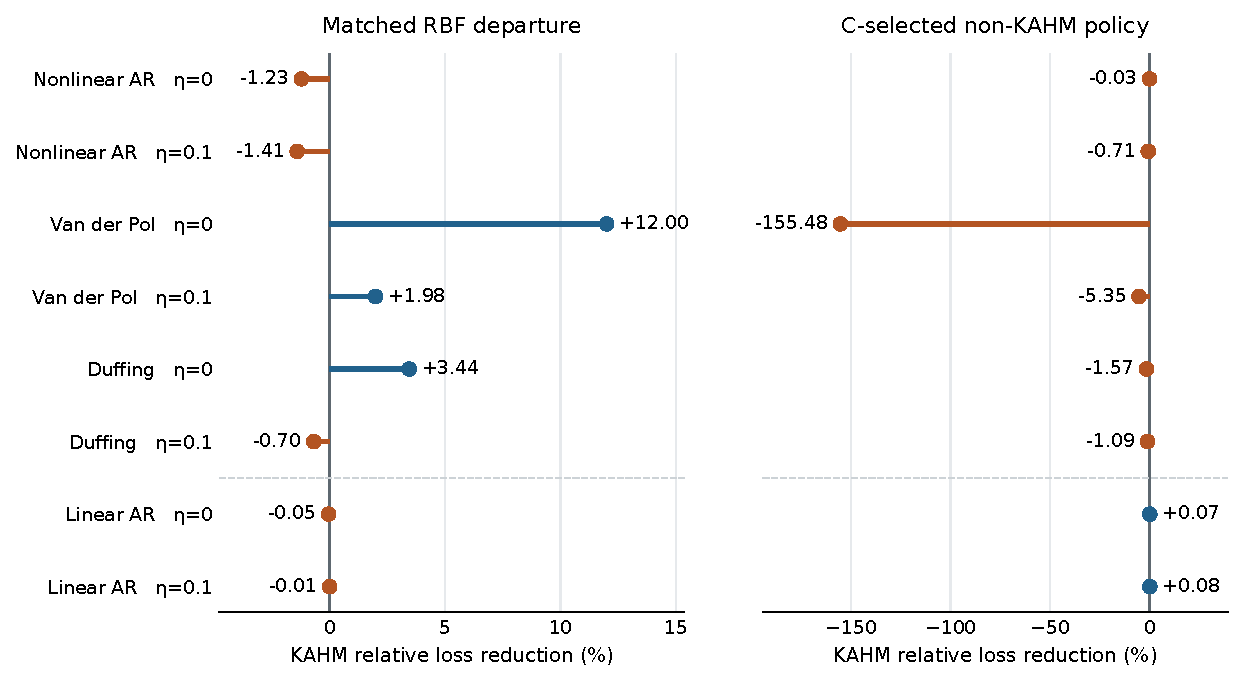
\includegraphics[width=\linewidth]{generated/reconstruction_mechanism/law_noise_contrasts.pdf}
\caption{Condition-specific gains of bounded KAHM departure over the
matched bounded RBF departure and the C-selected non-KAHM procedure.
Each point is $100(1-\overline L_K/\overline L_m)$, where the bars denote
mean loss over 24 repetitions of that condition. Positive values favor
KAHM. The panels use different horizontal scales, and labels give the
point estimates. These descriptive estimates have no condition-specific
confidence claims. The dashed divider separates nonlinear laws from
the linear negative control.}
\label{fig:mechanism-conditions}
\end{figure}

The maximum taskwise KAHM-to-ridge maximum-error ratio is
\RMMaxErrorRatio{}, below the limit of five. There are
\RMFeatureViolations{} feature-bound, \RMCoefficientViolations{}
coefficient-bound, and \RMCorrectionViolations{} correction-bound
violations. C selects a nonzero KAHM correction weight in
\RMKActiveNonlinear{} of 432 nonlinear task--horizon combinations and
\RMKActiveLinear{} of 144 linear-control combinations. This activation
frequency describes calibration choices, not a guarantee of lower D loss.
Mean charged fitting and selection time is \RMKFitSeconds{} seconds
for bounded KAHM departure and \RMRFitSeconds{} seconds for bounded RBF
departure. Appendix~\ref{app:reconstruction-results} reports prediction
time, retained model size, and the accounting boundaries.

The algebraic example, deterministic bound, and empirical comparisons
answer different questions. A distinct feature can be poorly aligned
with the target or difficult to estimate from the available sample.
A bounded correction can remain inaccurate. An unresolved improvement
margin does not establish equality of the representations. The
conclusions therefore apply to the specified reconstructions, decoder,
selection rules, and observation laws.

\section{Training local reconstruction for forecasting}
\label{sec:direct-reconstruction}

The reconstruction-departure experiment uses fixed local geometry. A
complementary experiment asks whether forecasting error can usefully train
the KAHM reconstruction and its gates. We compare this intervention with
gate training alone and with equally parameterized interventions in three
non-KAHM local models. The implementation, task roster, prepared inputs,
and analysis were publicly archived before evaluation on split D. The
design was informed by earlier experiments; the archive is a prospective
execution checkpoint, rather than an external preregistration.

\subsection{Horizon-specific reconstruction and residual prediction}

For a scalar series observed through time $t$, let
$x_t=(y_{t-L+1},\ldots,y_t)^\top\in\R^L$ be the history and
$y_{t+h}$ the target at forecast offset $h$. Training standardization gives
$z_t\in\R^L$. Each local model $c$ has $m_c$ reference histories stored as
the rows of $Q_c\in\R^{m_c\times L}$, their mean
$\mu_c=m_c^{-1}Q_c^\top\mathbf1$, and an orthonormal principal basis
$P_c\in\R^{L\times r_c}$. Three partition blocks request 2, 4, and 8
local models, respectively, with at most 24 references and effective
rank $r_c\leq2$ per model. The reference sets, principal directions,
and positive kernel regularizers $\lambda_c$ are fitted on split A.

Let $f_{0,h}$ be a raw-history ridge forecast fitted on A. For gate family
$g$, the corrected forecast is
\begin{equation}
 \widehat y_{t+h}=f_{0,h}(x_t)+\gamma_h
 \left\{a_h+\beta_h^\top
       \widetilde\Gamma_{g,h}(z_t;\theta_h)\right\},
 \qquad \gamma_h\in\{0,1/4,1/2,1\}.
 \label{eq:direct-forecast}
\end{equation}
Here $\Gamma_{g,h}$ concatenates the gates and gated principal coordinates
of Equation~\eqref{c:eq:local}; the tilde denotes column standardization
fitted on A. The scalar $a_h$ is an unpenalized intercept, and $\beta_h$
is a coefficient vector of the same dimension as the feature map.
The baseline penalty is selected by an inner split of A, after which
the baseline is refitted on A and held fixed. Each local model therefore
learns residuals of the same baseline.

For block $b$ and horizon $h$, the parameter
$\xi_{b,h}\in[-\log4,\log4]$ changes the kernel bandwidth. With
$\Sigma_c$ the positive-definite covariance of the projected reference
coordinates, define
\[
 D_{c,ij}=\frac{\|\Sigma_c^{-1/2}P_c^\top(q_{ci}-q_{cj})\|_2^2}{2r_c},
 \qquad
 d_{c,i}(z)=\frac{\|\Sigma_c^{-1/2}P_c^\top(z-q_{ci})\|_2^2}{2r_c},
\]
where $q_{ci}\in\R^L$ is reference $i$ as a column vector. For $r_c>0$,
\begin{align}
 K_c(\xi)_{ij}&=\exp\{-D_{c,ij}e^{-2\xi}\},&
 k_c(z;\xi)_i&=\exp\{-d_{c,i}(z)e^{-2\xi}\},\nonumber\\
 w_c(z;\xi)&=(K_c(\xi)+\lambda_c I_{m_c})^{-1}k_c(z;\xi),&
 r_c^{\mathrm{K}}(z;\xi)&=
 \frac{Q_c^\top w_c(z;\xi)}{\mathbf1^\top w_c(z;\xi)}.
 \label{eq:direct-kahm}
\end{align}
A rank-zero local model returns its center. A second parameter
$\eta_{b,h}\in[-\log4,\log4]$ multiplies the block's gate logits by
$e^{\eta_{b,h}}$ before softmax normalization. Thus $\theta_h$ contains
three bandwidth parameters and three gate-temperature parameters.
Zero parameters recover the fixed model.

Bandwidth changes affect both the reference Gram matrix and the query
kernel vector. To see their effects explicitly, suppress local indices,
write $M=K+\lambda I$, $w=M^{-1}k$, $s=\mathbf1^\top w$, and
$r=Q^\top w/s$. Differentiating $Mw=k$ and then the quotient gives
\begin{equation}
 dw=M^{-1}(dk-dM\,w),\qquad
 dr=\frac{(Q^\top-r\mathbf1^\top)\,dw}{s}.
 \label{eq:direct-derivative}
\end{equation}
These identities require invertible $M$ and $s\ne0$. They also show why
a small signed normalizer can amplify changes in the reconstruction.
The implementation shifts query log kernels to avoid common underflow
and rejects candidates for which
$|\sum_i w_i|/\sum_i|w_i|\leq10^{-10}$ on A, B, or C. This ratio
is defined as zero when all weights vanish. If a selected model fails this check on D, the
baseline supplies forecasts for the entire affected horizon.

\subsection{Selection, controls, and evaluation}

For each geometry candidate and $\alpha\in\{0.01,0.1,1\}$, a ridge
head minimizes the sum of squared A residuals plus
$\alpha\|\beta_h\|_2^2$. Geometry training minimizes B forecast MSE
at $\gamma_h=1$, normalized by an A-only target-variance scale.
Split C chooses the penalty and correction weight separately for each
horizon; the zero correction is retained unless a candidate has strictly
smaller C error. Split D evaluates the selected forecasts. Its labels
are unavailable to every fitting and selection step.

Affine, locality, and RBF-local controls each train three shape parameters
and three gate temperatures. The shape changes are, respectively, a
principal-projection gain, a balance between projection residual and
center distance, and tangent/normal anisotropy. Appendix~\ref{app:direct-protocol}
defines these maps. Fixed, gate-trained, and shape-trained versions of
the four families give twelve geometric procedures. Raw ridge, raw
Nystr\"om RBF, histogram boosting, seasonal naive, and a C-selected
non-KAHM policy complete the 17-method comparison. The policy chooses
one complete method from its C error and is charged for all candidate
computations. Each geometry optimization has the same 256-evaluation
ceiling per horizon and penalty. Equal parameter counts and evaluation
limits do not imply equal function classes or wall time.

The synthetic evaluation uses twelve independent repetitions of each of
the nonlinear AR, Van der Pol, and Duffing laws. A/B/C/D contain
64/32/32/128 independent episodes of length 72. Histories have length 12
and offsets are 1, 4, and 12; A/B/C are capped at 512/256/256 rows,
and D contains 1,664 origins. The 18 primary contrasts compare
reconstruction-trained KAHM with raw RBF, gate-trained KAHM, each of the
three shape-trained local controls, and the non-KAHM policy on each law.
Two-sided Bonferroni-adjusted Student intervals use twelve paired
repetition differences and 11 degrees of freedom. Their simultaneous
coverage relies on the stated normal approximation and applies only to
this family.

The natural evaluation selects ten series from Dominick retail,
rideshare prices, Wikipedia traffic, and Sunspot daily data
\citep{Godahewa2021Monash}. Selection uses training-prefix eligibility
and fixed identifier hashes. Chronological A/B/C/D segments contain
50/20/15/15 percent of each series; missing windows are omitted without
interpolation. The three selected rideshare series have no complete B
windows. Consequently, the planned four-collection aggregate is
undefined. The available seven series support a separate descriptive
comparison that weights series equally within each of three collections
and then weights the collections equally. Full source details, selection
chronology, scaling, and the preceding nine-task gate-training pilot
appear in Appendix~\ref{app:direct-protocol}.

\subsection{Predictive results and computational cost}

All \DirectAvailableTasks{} feasible tasks completed, producing
\DirectAvailableOutputs{} of \DirectPlannedOutputs{} planned
method--task records. The 51 unavailable records belong to the three
rideshare tasks. No additional task failures, invalid objective
evaluations, or numerical fallbacks occurred. Replay of the saved
selected states and a separate calculation of the losses and intervals
verified the reported results; these checks establish computational
consistency, not independent experimental replication.

\begin{table}[t]
\centering\small
\setlength{\tabcolsep}{5pt}
\caption{Direct-reconstruction forecasting results. Synthetic entries are
mean MSE over twelve repetitions per law. Natural entries average scaled
MSE equally over the three available collections, after averaging within
collection. The planned four-collection aggregate is undefined.
``Reconstruction'' denotes the corresponding shape intervention for
non-KAHM controls.}
\label{tab:direct-methods}
\begin{tabular}{lrrrr}
\toprule
Procedure & Nonlinear AR & Van der Pol & Duffing & \shortstack{Natural subset\\scaled MSE} \\
\midrule
Ridge & 0.005304 & 0.045166 & 0.007212 & 0.38563 \\
Raw RBF & 0.0049509 & 0.0064823 & 0.0043907 & 0.36301 \\
Boosted trees & 0.005059 & 0.0024251 & 0.0077638 & 0.3522 \\
Seasonal naive & 0.0088262 & 0.29404 & 0.040538 & 0.46013 \\
Fixed KAHM & 0.0048288 & 0.022324 & 0.0061418 & 0.39407 \\
Fixed affine & 0.0048524 & 0.018702 & 0.0053904 & 0.38001 \\
Fixed locality & 0.0048879 & 0.015133 & 0.005206 & 0.37626 \\
Fixed RBF-local & 0.0047977 & 0.017581 & 0.0058852 & 0.3862 \\
Gate KAHM & 0.004813 & 0.014554 & 0.0056708 & 0.39619 \\
Gate affine & 0.0048022 & 0.010615 & 0.0050184 & 0.38952 \\
Gate locality & 0.0048618 & 0.013712 & 0.0045407 & 0.38233 \\
Gate RBF-local & 0.0047522 & 0.011134 & 0.0059965 & 0.36779 \\
Reconstruction KAHM & 0.0048087 & 0.0085249 & 0.0053583 & 0.37194 \\
Reconstruction affine & 0.0048034 & 0.0075449 & 0.0047109 & 0.38172 \\
Reconstruction locality & 0.0048625 & 0.0092922 & 0.0043984 & 0.37483 \\
Reconstruction RBF-local & 0.0048001 & 0.0077975 & 0.0050204 & 0.36383 \\
Selected non-KAHM & 0.0047666 & 0.0024251 & 0.0041435 & 0.38247 \\
\bottomrule
\end{tabular}

\end{table}

Reconstruction training lowers KAHM's mean synthetic MSE relative to
its fixed version by 0.42\%, 61.81\%, and 12.76\% on AR, Van der Pol,
and Duffing, respectively. Relative to gate training alone, the
reductions are 0.09\%, 41.43\%, and 5.51\%. Of the 18 primary
intervals, \DirectPrimaryPositive{} favor KAHM,
\DirectPrimaryNegative{} favor its comparator, and
\DirectPrimaryUnresolved{} include zero
(Figure~\ref{fig:direct-primary}). The favorable contrasts are against
raw RBF on AR, with a 2.87\% reduction and absolute MSE-difference
interval $[6.65\!\times\!10^{-6},2.776\!\times\!10^{-4}]$, and against
gate-trained KAHM on Van der Pol, with a 41.43\% reduction and interval
$[0.004349,0.007709]$. Differences are comparator MSE minus KAHM MSE.

Shape-trained affine and the selected policy are more accurate than
KAHM on Van der Pol; the policy selects boosting in all twelve
repetitions. Raw RBF, shape-trained affine, shape-trained locality,
and the policy outperform KAHM on Duffing. No favorable primary
interval compares KAHM with an equally shape-trained non-KAHM local
control. Direct training therefore improves KAHM in some settings,
particularly Van der Pol, without establishing an advantage specific
to its reconstruction rule. Intervals containing zero leave their
comparisons unresolved and do not establish equivalence.

\begin{figure}[t]
\centering
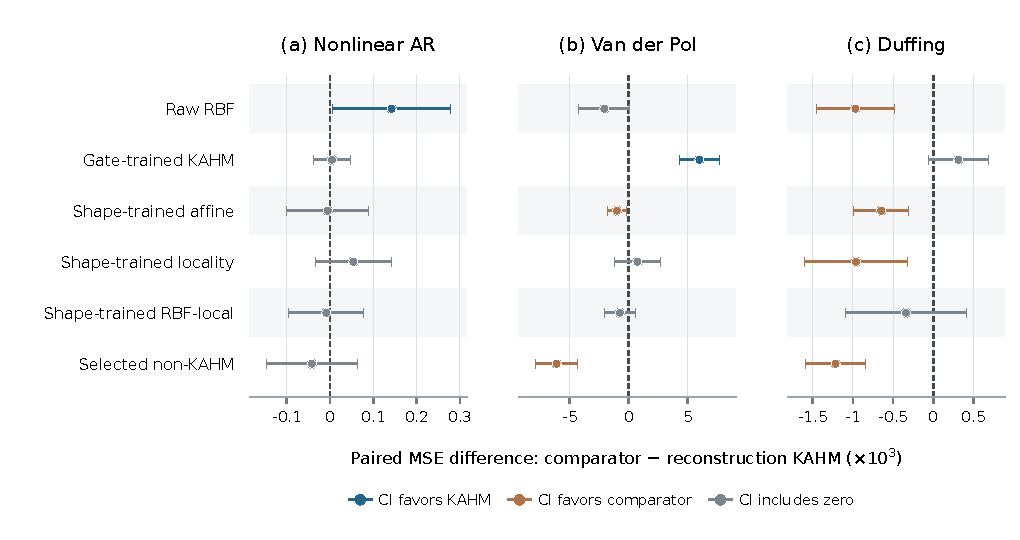
\includegraphics[width=\linewidth]{generated/direct_reconstruction/primary_contrasts.pdf}
\caption{All 18 primary direct-reconstruction contrasts. Points and
intervals show comparator-minus-KAHM MSE multiplied by 1,000. Blue
intervals favor KAHM, orange intervals favor the comparator, and gray
intervals contain zero. Two-sided Bonferroni-adjusted Student intervals
use twelve paired repetitions per law and 11 degrees of freedom.
Panel scales differ.}
\label{fig:direct-primary}
\end{figure}

On the available natural collections, KAHM has scaled MSE $0.371935$,
compared with $0.385625$ for ridge, a 3.55\% reduction. Raw RBF
($0.363007$), boosting ($0.352201$), and shape-trained RBF-local
($0.363835$) are more accurate. The ridge gain is concentrated in
Dominick; excluding that collection leaves a 0.00229\% improvement
across the other two collections. Twelve of the 21 available natural
horizons select zero KAHM correction, including every Sunspot horizon.
Table~\ref{tab:direct-natural} reports all collection-specific results.

The \DirectOptimizations{} geometry fits use
\DirectObjectiveEvaluations{} objective evaluations. Of these fits,
2,491 report convergence, 604 reach their evaluation budget, and one
has an abnormal optimizer stop; each retains its best finite candidate.
Mean synthetic pipeline time is 10.725\,s for reconstruction-trained
KAHM, 0.914\,s for gate-trained KAHM, 0.0774\,s for fixed KAHM,
0.0172\,s for raw RBF, and 0.653\,s for boosting. On the seven
available natural tasks, KAHM averages 7.929\,s, compared with
0.0130\,s for raw RBF and 0.655\,s for boosting.
Table~\ref{tab:direct-cost} and Figure~\ref{fig:direct-natural-cost}
report the complete accuracy and resource comparison. These costs
include model fitting, selection, querying, and state serialization;
they do not measure online update latency.

\section{Budgeted online adaptation: a completed development decision}
\label{sec:adaptive-development}
% Generated numerical macros from the amended adaptive development evidence.
\providecommand{\ADRunCount}{144}
\providecommand{\ADForecastCount}{387{,}900}
\providecommand{\ADAuditChecks}{6{,}713{,}837}
\providecommand{\ADSmallKRRExcess}{22.26}
\providecommand{\ADSmallPninetyNine}{9.89}
\providecommand{\ADLargeKRRExcess}{9.22}
\providecommand{\ADLargePninetyNine}{11.75}
\providecommand{\ADOverruns}{4}
\providecommand{\ADServiceSteps}{21{,}662}
\providecommand{\ADPeakPrediction}{175{,}555.08}
\providecommand{\ADPeakTruth}{-0.9815}
\providecommand{\ADQueryFeatureMagnitude}{3.20}
\providecommand{\ADReplayFeatureMagnitude}{392}
\providecommand{\ADRelativeDenominator}{0.354}


\paragraph{Question and scope.}
A subsequent development study tested whether updates to local KAHM geometry under fixed reference and
replay budgets provide enough predictive benefit to justify a larger evaluation.
The complete design comprises twelve streams, six methods and two capacity
tiers: \ADRunCount{} runs and \ADForecastCount{} scored forecasts after the
numerical amendment described below. Four stationary nonlinear AR streams
are paired by innovations with four recurring A/B streams; the latter
alternate regimes every 256 observations, and both regimes occur in the
initial fitting prefix. Regime labels are never supplied to the forecasters.
Three Dominick weekly series and one Sunspot daily series are deliberately
reused from previously inspected inputs. This supplies development evidence
from one generator and two selected natural collections, with no claim of
new-source confirmation. Appendix~\ref{app:adaptive-development} records
the chronology, decision thresholds and source identities.

\paragraph{A simpler adaptive prototype.}
All geometric methods retain a sliding-window raw ridge baseline and
residual heads. Fixed KAHM updates its heads with unchanged initial geometry;
adaptive KAHM, affine and RBF-local share the bounded reference-refresh
policy. Each adaptive refresh coherently re-encodes replay histories and
rebuilds residual heads. The sixth method is sliding-window Gaussian kernel
ridge with a free intercept and recursive add/delete inverse updates. Its
forecast also uses the calibrated blend with raw ridge: correction weight
one gives the kernel prediction and zero gives raw ridge. Thus the reported
KRR arm is a selected forecasting procedure, not an unblended kernel forecast
on every horizon, and it is not the published KRLS-T algorithm.
The small tier allows 64 shared
geometric references and 128 replay rows per horizon, and the large tier
allows 128 and 256. Kernel supports are capped separately per horizon;
these quotas are not equal byte or computational allocations. Bandwidths
and gate temperatures are fixed, so this prototype is not a streaming
reproduction of the forecast-trained model in the preceding study.

\paragraph{Chronology and numerical amendment.}
The first 35\% of each stream initializes the model, 35--50\% supplies
chronological calibration, and the latter half supplies evaluation.
Only matured labels enter an update. Forecasts are recorded before their
targets arrive and remain immutable. Each horizon selects a correction
weight from $\{0,0.25,0.5,1\}$ on matured calibration targets, then retains
that weight during evaluation. The original complete attempt had four
correction-head failures and 8,659 framework fallback forecasts. Amendment
A1 replaces accumulated correction normal equations with a centered,
column-equilibrated augmented ridge solve using pivoted QR, preserving
the objective, penalties, data, scalers, reference policy and decision
rules. All geometric arms receive the repair, and the full roster is
repeated. The amended runs have no unexpected model exceptions, framework
fallback forecasts or observed cap violations. Both attempts are preserved;
their source freezes were local checkpoints, not public preregistration.
The repeat follows observed outcomes and is not independent confirmation.

% Generated from saved amended development evidence; no model fitting.
\begin{table}[!htbp]
\centering\small\setlength{\tabcolsep}{5pt}
\caption{Budgeted adaptive development study: scaled MSE, lower is better. Origins are averaged within horizon, horizons within series, and series within collection. The natural mean gives Dominick and Sunspot equal weight. The two capacity tiers are quotas, not equal-byte allocations. All non-ridge arms, including KRR, use calibration-selected mixing with the common ridge baseline. No losses are pooled with earlier studies.}
\label{tab:adaptive-development-loss}
\begin{tabular}{@{}lrrrrr@{}}
\toprule
Method & Stationary & Recurring & Dominick & Sunspot & Natural mean \\
\midrule
\multicolumn{6}{l}{\textit{Small: 64 shared references / 128 replay rows per horizon}} \\
Raw ridge & 2.2402 & 3.4583 & 1.6144 & 2.3697 & 1.9920 \\
Fixed KAHM & 2.2407 & 3.4583 & 1.6134 & 2.3697 & 1.9915 \\
Adaptive KAHM & 2.2399 & 3.4583 & 1.6135 & 2.3697 & 1.9916 \\
Adaptive affine & 2.2407 & 3.4583 & 1.6137 & 3.4004 & 2.5071 \\
Adaptive RBF-local & 2.2428 & 3.4583 & 1.6160 & 2.3697 & 1.9928 \\
Sliding-window KRR & 2.2491 & 3.3578 & 0.8685 & 2.3897 & 1.6291 \\
\midrule
\multicolumn{6}{l}{\textit{Large: 128 shared references / 256 replay rows per horizon}} \\
Raw ridge & 2.0275 & 3.3623 & 0.8471 & 2.1045 & 1.4758 \\
Fixed KAHM & 2.0375 & 3.4031 & 0.8464 & 2.1045 & 1.4754 \\
Adaptive KAHM & 2.0280 & $1.376\times 10^{8}$ & 0.8444 & 2.1045 & 1.4744 \\
Adaptive affine & 2.0364 & $1.061\times 10^{6}$ & 0.8446 & 2.2085 & 1.5266 \\
Adaptive RBF-local & 2.0290 & 3.7036 & 0.8460 & 2.1045 & 1.4752 \\
Sliding-window KRR & 2.0551 & 3.2079 & 0.5954 & 2.1045 & 1.3499 \\
\bottomrule
\end{tabular}
\end{table}


\paragraph{Predictive outcome.}
Table~\ref{tab:adaptive-development-loss} reports MSE divided by an
initial-prefix seasonal-difference scale. The scale and online schedule
differ from earlier sections, precluding direct comparisons of their
numerical scores. Both complete tiers fail the recurring and natural-data
accuracy criteria and receive the decision \textsc{Defer}. Adaptive KAHM's
natural mean loss exceeds kernel ridge by \ADSmallKRRExcess\% at the small
tier and \ADLargeKRRExcess\% at the large tier. At each tier, only two of
twelve natural horizon/series combinations activate a KAHM correction;
every Sunspot horizon selects zero. Small-tier recurring corrections are
all zero, while nine of twelve large-tier recurring corrections are active.
Baseline recovery at zero correction does not demonstrate added geometric
value. The descriptive advancement criteria are development triage rules,
not a hypothesis test or a universal definition of effectiveness.

\paragraph{Extrapolation persists after the numerical repair.}
For recurring seed 20261101, origin 1554 and horizon 12, large-tier adaptive
KAHM predicts $\ADPeakPrediction$ when the target is $\ADPeakTruth$.
At the preserved diagnostic state, the largest absolute standardized query
feature is about $\ADQueryFeatureMagnitude\times10^6$, compared with
$\ADReplayFeatureMagnitude$ in the current supervised replay. A fresh
centered SVD solve reproduces the large correction. The minimum relative
signed denominator, defined by the ratio in
Equation~\eqref{eq:mechanism-relative-denominator}, is
$\ADRelativeDenominator$, safely above its $10^{-10}$
guard. Adaptive affine also exhibits severe extrapolation under a fresh
solve. These post-run observations identify a representation--decoder
stability problem in the examined states. They are consistent with a
query falling outside the observed feature range of matured-label replay, but do not
isolate the causal contributions of scaling, label delay and geometry
refreshes. No forecasts were removed, clipped or retuned to obtain the
reported decision.

\paragraph{Cost and research consequence.}
Adaptive KAHM passes the monitored 20\,ms p99 screen on every stream:
the worst per-stream values are \ADSmallPninetyNine{} and
\ADLargePninetyNine{}\,ms. There are nevertheless \ADOverruns{} service
intervals above 20\,ms among \ADServiceSteps{} evaluation observation
steps; the screen is not an enforced per-step deadline. Service includes
updates, geometry refreshes, feature/head rebuilds and prediction, but
excludes evidence serialization and scoring. The eager prototype maintains
geometry even when its correction is disabled. Resource details appear
in Table~\ref{tab:adaptive-development-resources}.
This result establishes measured implementation feasibility under the
stated screen while withholding support for an adaptive forecasting
advantage. The fixed-geometry reconstruction-departure experiment in
Section~\ref{sec:reconstruction-mechanism} subsequently tests a distinct
readout and an explicit correction bound. Its result is reported separately,
rather than treated as a repair or confirmation of the adaptive prototype.
The development outcome does not rule out every other adaptive or
forecast-trained KAHM formulation.

\section{Conditional gains in controlled forecasting}\label{c:sec:capacity}

The controlled forecasting laws are nonlinear autoregression (AR),
Van der Pol, and Duffing. Each repetition independently generates 128
training, 128 validation, and 512 test episodes of length 72. Histories
have length 12 and predict offsets 1, 4, and 12 at 13 origins per episode.
Entire episodes stay within a split; MSE averages origins and horizons
within episodes and then episodes. Appendix~\ref{c:app:methods} specifies
the numerical generators and fitting rules.

The first study has 24 full data-and-fit repetitions in each of nine
primary settings: six target functions on the branch construction and three forecasting laws. Adding
local coordinates to KAHM affinities improves ridge prediction beyond the
fixed practical margin in \LocalPracticalBenefitCount{} settings. On Van
der Pol, mean MSE falls from $\VDPPhiRidgeMSE$ to
$\VDPKAHMLocalRidgeMSE$, although affine local coordinates perform better
with the same ridge head. The first study uses 95\% Bonferroni-adjusted paired Student intervals
for a family of 29 contrasts. This supports retaining local position,
while leaving the complete representation--decoder choice unresolved.

A follow-up specifies its candidate models, practical margins, and
analysis before generating 24 additional independent repetitions per
forecasting law. It compares raw histories, affine local features, KAHM local features,
and full KAHM scores with 64 or 256 Gaussian Nystr\"om landmarks. The
head appends linear coordinates to the finite nonlinear basis, standardizes
basis columns, and uses an ordinary Euclidean ridge penalty. Validation
selects among three bandwidth multipliers and seven penalties; the fitted
model uses training observations only. Equal landmark counts do not imply
equal realized ranks, function classes, or computational costs.

\begin{table}[t]
 \caption{The twelve primary comparisons of finite-decoder capacity. Entries are
 mean MSEs and paired differences over 24 independent full repetitions,
 multiplied by $10^3$; $\Delta$ is control minus KAHM-local loss. Intervals
 use the follow-up's separate 95\% Bonferroni paired Student family.
 Coverage relies on normality or its approximation for paired differences;
 these are not distribution-free guarantees.}
 \label{c:tab:capacity}
 \centering\small\setlength{\tabcolsep}{3pt}
 % Generated by scripts/build_paper_assets.py; do not edit.
\begin{tabular}{lrlrrl}
\toprule
System & $M$ & Control & Control MSE & KAHM local MSE & $\Delta$ [interval] \\
\midrule
Nonlinear AR & 64 & Raw & 4.4238 & 4.8795 & $-0.4556\;[-0.5235,\,-0.3878]$ \\
Nonlinear AR & 64 & Affine local & 4.9120 & 4.8795 & $0.0325\;[-0.0031,\,0.0680]$ \\
Nonlinear AR & 256 & Raw & 4.6958 & 5.1749 & $-0.4791\;[-0.6013,\,-0.3569]$ \\
Nonlinear AR & 256 & Affine local & 5.2347 & 5.1749 & $0.0598\;[-0.0131,\,0.1327]$ \\
\midrule
Van der Pol & 64 & Raw & 2.8586 & 1.0266 & $1.8320\;[1.7369,\,1.9271]$ \\
Van der Pol & 64 & Affine local & 1.3767 & 1.0266 & $0.3501\;[0.2755,\,0.4247]$ \\
Van der Pol & 256 & Raw & 1.6541 & 0.8720 & $0.7822\;[0.7550,\,0.8094]$ \\
Van der Pol & 256 & Affine local & 1.0780 & 0.8720 & $0.2060\;[0.1810,\,0.2311]$ \\
\midrule
Duffing & 64 & Raw & 3.4597 & 4.2154 & $-0.7557\;[-1.0831,\,-0.4282]$ \\
Duffing & 64 & Affine local & 3.0549 & 4.2154 & $-1.1605\;[-1.4707,\,-0.8503]$ \\
Duffing & 256 & Raw & 2.8364 & 4.0736 & $-1.2372\;[-1.5242,\,-0.9503]$ \\
Duffing & 256 & Affine local & 2.7981 & 4.0736 & $-1.2756\;[-1.5702,\,-0.9810]$ \\
\bottomrule
\end{tabular}

\end{table}

Table~\ref{c:tab:capacity} reports the complete comparison family. KAHM local features outperform raw and affine local features
on Van der Pol at both widths in every repetition. At 256 landmarks,
mean MSEs are $\VDPKAHMWideMSE$, $\VDPRawWideMSE$, and
$\VDPAffineWideMSE$, respectively: descriptive reductions of
\VDPRawWideRelativeGain\% and \VDPAffineWideRelativeGain\% relative to the
controls. The two simultaneous lower endpoints, $0.00075496$ and
$0.00018100$, exceed the prespecified practical margin $0.00014891$; both
64-landmark comparisons also clear it. Raw inputs win on AR at both
widths, and both controls win on Duffing. KAHM--affine differences on AR
remain unresolved. The separate 29- and 12-contrast families do not imply
a joint 95\% coverage statement. Their inferential units are complete
repetitions, not windows or horizons (Appendix~\ref{c:app:statistics}).

\paragraph{Numerical sensitivity and an adverse natural-data check.}
\label{c:sec:numerical}
The original Gaussian query evaluation can produce an all-zero row before
signed normalization. Writing $\ell_j$ for a query log-kernel entry, replacing
$\exp\ell_j$ by
$\exp(\ell_j-\max_i\ell_i)$ preserves exact normalized weights whenever
the denominator is nonzero (Proposition~\ref{c:prop:inner-scaling}). In a
post-hoc check reusing the 24 Van der Pol follow-up samples and banks, with
affected heads refitted and validation-tuned, exactly zero normalizers fall
from \NumericalOriginalZeroCount{} among \NumericalQueryClusterCount{}
query--local-model evaluations to zero. KAHM-local mean MSE changes by
less than $4\times10^{-13}$ at either width, whereas full-score losses
improve by roughly $0.37$--$0.39\%$. Row scaling addresses this underflow
pathway; it does not prevent signed cancellation or establish stability on independently generated data.

On a fixed grouped split of Airfoil Self-Noise \citep{Brooks1989Airfoil},
raw RBF obtains mean group-weighted MSE $\AirfoilRawRBFMSE$ dB$^2$,
compared with $\AirfoilKAHMLocalRBFMSE$ for KAHM-local RBF. The validation selector chooses
raw RBF in all 24 fits. These seeds characterize fitting variability on
one static-regression dataset and split, not independent natural
forecasting evidence. Together, the controlled results motivate testing
local features as conditional candidates. The branch symmetry result does not explain the Van der Pol gain,
and these simulations do not establish transfer to new source families;
Section~\ref{sec:natural} examines that question separately.

\section{Natural forecasting: transfer, cost, and predicting benefit}\label{sec:natural}

\subsection{A separate source-level evaluation}
The natural study fixes four development families (Electricity, NN5,
Tourism, and FRED-MD) and four confirmation families (Traffic, Hospital,
Saugeen River flow, and US births). Versions, licenses, eligibility rules,
and chronological windows are specified in Appendix~\ref{sec:nf-protocol}.
Training-prefix eligibility and a fixed salted ordering select 26 series.
Two history--horizon regimes, two capacities, and two seeds yield 208 runs:
128 development and 80 confirmation. Related series, windows, horizons,
capacities, and seeds remain within their original source families.
The units describing transfer breadth are the four confirmation families.

Each series uses chronological 60/20/20 percent training/validation/test
blocks, and every target horizon lies entirely within its split. All
learned transformations and feature bases use the permitted training
data. Validation chooses hyperparameters; a final refit uses eligible
pretest targets, and test outcomes never retune parameters. Contexts can
use earlier observed values. At most 64 validation and 64 test origins
are retained by a fixed spacing rule; missing windows are excluded
identically for every method, without interpolation or replacement series.
Mean-squared forecast error is divided by a fixed initial-training
seasonal-difference scale. Aggregation gives each source family equal
weight, followed by its nested task levels. These descriptive quantities
are not pooled with the controlled-study confidence families.

The twelve candidates include raw ridge and raw finite-RBF predictors;
affine-, locality-, and KAHM-gated local predictors, with and without the
full raw history; and seasonal naive, Holt, histogram boosting, and a small
MLP. The primary matched pair is raw RBF ($R$) versus raw plus KAHM ($K$).
The raw-augmented code is
\begin{equation}\label{eq:natural-raw}
 T_{\mathrm{raw}+g}(x)=\bigl(z(x),\,\phi_g(z(x)),\,
       (\phi_{g,c}(z(x))P_c^\top(z(x)-\mu_c))_c\bigr).
\end{equation}
It retains every standardized history coordinate. For a fixed fitted state
the raw input is therefore recoverable and Bayes information is unchanged
(Proposition~\ref{prop:nf-raw-preservation}). Finite fitted performance
can still change: appended features alter Gaussian distances, the
Nystr\"om basis, and ridge regularization, and the resulting nonlinear
classes need not be nested.

Small/medium configurations cap training windows at 512/1,024 and RBF
landmarks at 32/64. Each method fits its own preprocessing and geometry;
affine/locality alternatives never fit a KAHM kernel. Within a method,
features and head statistics are reused across penalties $\{0.01,1,100\}$.
The selected model is refitted from scratch. These are specified finite
procedures, not equally timed or exhaustively tuned algorithms. Detailed
heads, practical controls, capacity caps, and numerical conventions appear
in Appendices~\ref{sec:nf-methods}--\ref{sec:nf-protocol}.

\subsection{Which computational work is charged?}
Measured warm-library pipelines include required preparation/loading,
preprocessing, validation search, selection bookkeeping, chosen refitting,
forecasting, and serialization. Libraries are initialized beforehand;
imports and process launch are separately exposed. Wall and CPU time,
model bytes, and process high-water memory have distinct recorded scopes.
Let $S_m$ denote method $m$'s search nodes, $F_m$ its final fit and forecast,
and $m^*$ a validation-selected candidate. Its charged work is
\begin{equation}\label{eq:main-cost}
 C_{\rm val}=\sum_{v\in\mathcal D_{\rm data}\cup
             (\bigcup_{m\in\mathcal A}S_m)\cup F_{m^*}}c_v
             +c_{\rm decision}.
\end{equation}
Unique dependency nodes are counted once. A diagnostic selector likewise
pays for all required descriptors and probes, even when it rejects KAHM.
Acquiring development labels and fitting the small diagnostic regressions
are separate offline investments. No assumed deployment count is used to
amortize them. The costs describe measured implementations on one CPU
environment; they are not intrinsic complexity or hardware-independent
speed ratios.

\subsection{Accuracy and cost on reserved sources}
All 208 declared runs completed with every candidate present; saved
forecasts reconstruct all 2,496 task--method losses. Table~\ref{tab:natural-main}
retains all twelve confirmation candidates. Raw plus KAHM has
\NaturalErrorIncrease\% higher aggregate error than raw RBF, at
\NaturalCostRatio{} times its measured warm-library pipeline cost. Raw
ridge has lower aggregate error than both. Against raw RBF, KAHM raises
mean loss by 0.50\% on Traffic, 12.27\% on Hospital, and 3.53\% on US births;
it lowers loss by 1.53\% on Saugeen, where raw ridge also performs better.
Leaving out any one confirmation family still leaves the KAHM aggregate
above raw RBF. This sensitivity check is descriptive and does not turn
four selected sources into a population-wide inference.

\begin{table}[t]
\centering\small
\caption{All twelve standalone methods on the reserved natural sources. Scaled MSE and warm-library wall time use equal source-family weights and the frozen within-source hierarchy. Times include required preprocessing, search, refitting, prediction, serialization, and measured bookkeeping; imports and launch are separate. These are descriptive results from four source families.}
\label{tab:natural-main}
\begin{tabular}{lrr}
\toprule
Method & Scaled MSE & Wall seconds per task \\
\midrule
Raw ridge & 0.7798 & 0.1880 \\
Raw RBF & 0.8075 & 0.1688 \\
Affine local & 0.9449 & 0.5002 \\
Locality local & 0.8964 & 0.2898 \\
KAHM local & 0.9354 & 0.3218 \\
Raw + affine & 0.8458 & 0.3379 \\
Raw + locality & 0.8462 & 0.2791 \\
Raw + KAHM & 0.8419 & 0.3874 \\
Seasonal naive & 1.0498 & 0.1614 \\
Holt & 2.3729 & 0.3449 \\
Histogram boosting & 0.9555 & 8.9103 \\
MLP & 0.8785 & 1.4626 \\
\bottomrule
\end{tabular}
\end{table}


The structural controls clarify attribution. Raw plus KAHM improves
aggregate loss over raw plus affine and raw plus locality by only 0.46\%
and 0.50\%, respectively. Each comparison favors KAHM on two source
means and the control on two; KAHM costs 14.65\% and 38.82\% more.
These mixed differences do not identify nonlinear reconstruction as a
general source of advantage. At the small/medium settings, KAHM raises
loss against raw RBF by about 2.00/6.70\%; the settings change both
sample caps and model sizes, so their effects are not separately identified.

The favorable development mean also needs qualification. KAHM reduced
loss against raw RBF by 42.45\%, but FRED-MD supplied 96.62\% of the
net absolute reduction. Removing that family reduces the apparent gain
to 4.65\%. Raw plus affine had lower mean loss and cost than KAHM in
each development family, and raw ridge had the lowest overall development
loss. Consequently, the development comparison alone did not establish
a KAHM-specific benefit.

Implementation overhead is substantial. Selection cleanup, including
explicit garbage collection, contributes 0.1381 of raw RBF's 0.1688 seconds
and 0.1825 of KAHM's 0.3874 seconds. Search and final refit are also
reported separately (Table~\ref{tab:cleanup-costs}). The 2.30-fold ratio
describes the supplied warm workflow; it is not a cold-start end-to-end
deployment ratio. Figure~\ref{fig:accuracy-cost} retains the full accuracy--cost
comparison, including selectors that must pay to choose a model.

\begin{figure}[t]
\centering
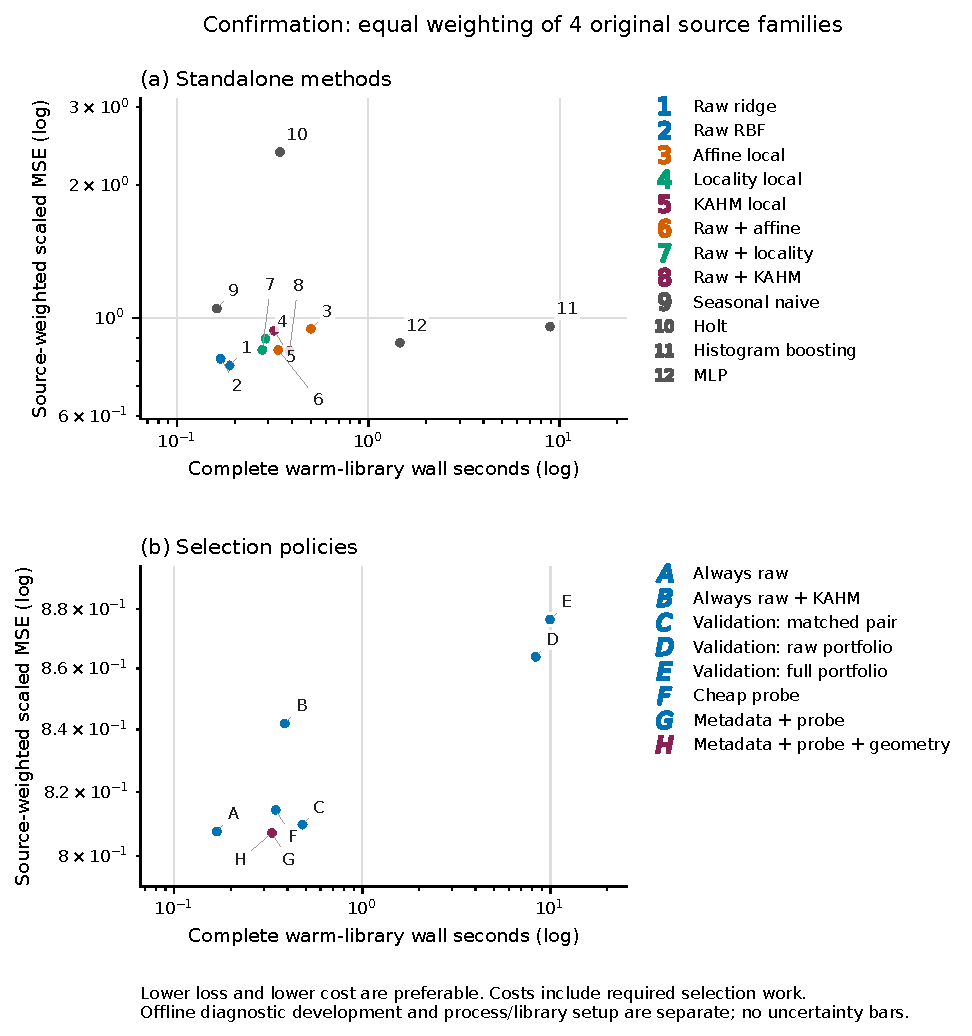
\includegraphics[width=\linewidth]{generated/natural/figures/accuracy_cost.pdf}
\caption{Reserved-source accuracy and measured warm-library cost. All points
use the same source hierarchy. The standalone and selector panels have
separate scales so that all declared candidates remain visible. Selector
costs include required searches and probes. Confirmation outcomes are used
to evaluate these procedures, not to fit a new selection rule.}
\label{fig:accuracy-cost}
\end{figure}

\subsection{The frozen benefit diagnostic}
Four fixed ridge diagnostics predict
$\log[(\ell_R+10^{-12})/(\ell_K+10^{-12})]$ from metadata $M$,
$M$ plus geometry $G$, $M$ plus a cheap validation probe $P$, or $M+P+G$.
Metadata describe training size, horizon/history ratio, and lag-one
autocorrelation; geometry adds gate entropy and an affine-projection
residual. The paid probe compares reduced-capacity raw/KAHM fits on
validation data. A positive estimated log benefit selects KAHM; ties
select raw. Development standardization and training hold out whole source
families. All variants are then fitted on development and frozen before
confirmation; confirmation outcomes cannot choose the variant or threshold.

The primary geometric increment, $M+P+G$ versus $M+P$, changes none of
the 80 confirmation decisions. Both achieve scaled MSE
\NaturalProbeLoss{} at about \NaturalProbeCost{} seconds. The probe already
computes the geometric descriptors, so they need no extra bank fit in this
pair. Log-benefit RMSE nonetheless increases from 0.184549 to 0.184680.
The shared decision rule improves aggregate loss over always raw by only
\NaturalProbeGainPercent\%, at \NaturalProbeCostRatio{} times its pipeline
cost. It improves one source mean, worsens one, and ties two.
Metadata-plus-geometry also makes exactly the same choices as metadata
alone, while paying for extra feature acquisition. All variants and
validation-portfolio controls remain in Table~\ref{tab:policy-summary}.

Offline learning requires more than fitting a small ridge regression.
Acquiring the matched development outcomes and shared probe/metadata
dependencies costs 80.83 seconds of summed measured pipeline work;
all four final ridge fits together add about 0.032 seconds. Shared
dependencies must not be added repeatedly across variants. These
observations provide no validated geometric adoption criterion for the
tested procedure. They also do not establish that usefulness is
unpredictable by a different, independently evaluated diagnostic.

\section{Post-hoc sensitivity to geometry scaling}\label{sec:scaling}
The preceding studies fix training z-score geometry scaling. To test whether
that choice determines their practical interpretation, a specified sensitivity analysis
replaces it with training min--max scaling to $[-1,1]$, without clipping future
inputs. The raw-history component and raw-input comparator remain standardized; all targets, splits,
seeds, head grids, capacities, and query conventions remain fixed. The protocol
and execution code were published before the sensitivity fits, after the
original outcomes had been inspected. These are paired post-hoc comparisons
on reused sources and draws, not fresh confirmation. Appendix~\ref{app:scaling}
specifies the intervention, costs, retained evidence, and complete results.
The previously fitted benefit diagnostic is not refitted or reevaluated for min--max
geometry.

\paragraph{Natural-source ranking.}
All 208 configurations are rerun for the three raw-augmented geometric
methods under both scalers, with unchanged raw RBF and ridge references.
On the four formerly reserved sources, KAHM's source-balanced scaled MSE
changes from \ScalingNaturalKahmStandardLoss{} to
\ScalingNaturalKahmMinmaxLoss{}, an increase of
\ScalingNaturalKahmChangePercent\% (Table~\ref{tab:scaling-natural}).
The min--max arm remains \ScalingNaturalKahmVsRawPercent\% above raw RBF
and \ScalingNaturalKahmVsRidgePercent\% above raw ridge. Min--max KAHM
beats raw RBF on only Saugeen, and raw ridge has lower loss on all four
source means. Leaving out any one family still leaves min--max KAHM
above raw RBF. Thus this specified scaling alternative does not reverse
the aggregate natural-data comparison.

% Generated by scaling_sensitivity/report.py from analysis/summary.json.
\begin{table}[t]
\centering
\small
\begin{tabular}{lrrr}
\toprule
Method & Standard MSE & Min--max MSE & Change (\%) \\
\midrule
Raw ridge & 0.7798 & 0.7798 & fixed \\
Raw RBF & 0.8075 & 0.8075 & fixed \\
Raw + affine & 0.8458 & 0.8596 & +1.62 \\
Raw + locality & 0.8462 & 0.8488 & +0.31 \\
Raw + KAHM & 0.8419 & 0.8422 & +0.03 \\
\bottomrule
\end{tabular}
\caption{Geometry-scaling sensitivity on the four formerly reserved natural sources. Scaled MSE uses the original source hierarchy. Standard arms reproduce the frozen results; min--max changes geometry only, retains the standardized raw-history component, and applies no input clipping. Change is $100(\ell_{\mathrm{minmax}}/\ell_{\mathrm{standard}}-1)$; negative favors min--max. Raw references are fixed. These comparisons are post-hoc sensitivity.}
\label{tab:scaling-natural}
\end{table}


The small aggregate change does not establish equivalent performance. KAHM's loss
falls by 0.15\% on Traffic and 0.86\% on Hospital, but rises by 0.90\% on
Saugeen and 0.35\% on US births. Small-capacity loss increases by 0.99\%,
whereas medium-capacity loss falls by 0.96\%; these settings still jointly
vary sample and model-size caps. The original development aggregate worsens
by 7.70\%, with heterogeneous source effects. The same intervention also
changes the affine and locality controls; it does not isolate an effect
of nonlinear KAHM reconstruction.

In the sensitivity execution, KAHM's source-balanced mean min--max warm method time is
\ScalingNaturalKahmMinmaxTime{} seconds per task, versus
\ScalingNaturalKahmStandardTime{} for standardized KAHM and
\ScalingNaturalRawTime{} for the remeasured raw RBF reference:
ratios of \ScalingNaturalKahmCostRatioStandard{} and
\ScalingNaturalKahmCostRatioRaw{}, respectively. These include search,
selection cleanup, refit, forecast, and serialization. A retained Saugeen
search/cleanup outlier contributes to the timing aggregate. They are
single-execution, implementation-specific observations, not an intrinsic
computational penalty of min--max scaling or a cold-start deployment claim.

\paragraph{Controlled finite-decoder comparisons.}
All 24 original complete draws for each law and both landmark counts are
reused. Both scaler arms retain raw, affine-local, KAHM-local, and KAHM-score
features; a matched locality-coordinate control is included.
Table~\ref{tab:scaling-controlled} reports every law/capacity cell, with
all representations and paired dispersion in Appendix~\ref{app:scaling}.
The main mean-loss ordering persists: raw RBF remains better than KAHM
local coordinates on autoregression and Duffing, whereas KAHM local coordinates remain better
than raw and both local controls on Van der Pol at both capacities.
KAHM-local scaling changes range from a 0.23\% increase on Van der Pol
at 256 landmarks to a 7.35\% reduction on Duffing at 256 landmarks.
The latter lowers MSE from $4.0736$ to $3.7741$ in units of $10^{-3}$,
but remains above raw ($2.8364$), min--max affine ($2.7742$), and min--max
locality ($2.6921$). Scaling can materially change an error without reversing
the scientific comparison. Because these comparisons reuse inspected draws, their reported
mean differences are descriptive.

% Generated by scaling_sensitivity/report.py from analysis/summary.json.
\begin{table}[t]
\centering
\scriptsize
\begin{tabular}{lrrrrrr}
\toprule
Law & $M$ & Raw & KAHM std. & KAHM min--max & Affine min--max & Locality min--max \\
\midrule
Nonlinear AR & 64 & 4.4238 & 4.8795 & 4.8678 & 4.8940 & 4.9414 \\
Nonlinear AR & 256 & 4.6958 & 5.1749 & 5.1584 & 5.1807 & 5.2577 \\
Van der Pol & 64 & 2.8586 & 1.0266 & 1.0248 & 1.3482 & 1.1240 \\
Van der Pol & 256 & 1.6541 & 0.8720 & 0.8740 & 1.0812 & 0.9448 \\
Duffing & 64 & 3.4597 & 4.2154 & 4.0951 & 2.9981 & 2.8227 \\
Duffing & 256 & 2.8364 & 4.0736 & 3.7741 & 2.7742 & 2.6921 \\
\bottomrule
\end{tabular}
\caption{Controlled geometry-scaling sensitivity on all 24 original complete draws per law and both landmark counts $M$. Mean MSE is multiplied by $10^3$. Raw inputs remain standardized; the min--max columns change only the fitted geometry scaler. Locality is the added matched coordinate control. These paired reused-draw comparisons are descriptive, with full dispersion and the score-only representation in Table~\ref{tab:scaling-controlled-all}.}
\label{tab:scaling-controlled}
\end{table}

\FloatBarrier

\section{Preserving raw forecasts while testing geometric utility}
\label{sec:utility-extension}

The preceding studies motivate a distinct question. Does KAHM help when
its contribution is a correction to an unchanged raw forecast, and how
does that contribution depend on training data and the raw decoder?
The extension separates these factors and tests a fixed adoption rule on
four additional archive collections. Its protocol, candidate grid, data
roster, and execution sources are frozen before its full model evaluations.
This is a prospective execution freeze, not external preregistration.
The earlier evidence and post-hoc scaling analysis remain separately
reported; no outcome from those archives is reclassified as new confirmation.

\subsection{Forecasts, controls, and selection}
\label{sec:utility-models}

The raw baseline is the inherited finite Gaussian Nystr\"om predictor with
appended linear history coordinates, column standardization, and a ridge
head. Its requested $M$ landmarks and regularization are fitted using the raw history
only. For each $g\in\{\mathrm{KAHM},\mathrm{affine},\mathrm{locality}\}$,
we fit a separate ridge head on the local-coordinate features of
Equation~\eqref{c:eq:local}, using the raw model's training residuals as
targets. The additive forecast is Equation~\eqref{eq:utility-additive}.
The correction has its own standardization and ridge penalty; it does not
change raw distances, landmarks, coefficients, or regularization, and it
introduces no additional Nystr\"om basis. Residuals are in-sample training
residuals, not cross-fitted residuals. This choice is part of the evaluated
procedure and can limit the structure left for the correction to learn.

All geometries use the same partitions, principal-direction configuration,
reference-selection rules, and fitting seeds. The geometry bank uses
three blocks of 2, 4, and 8 local models, requested rank two, at most 24
references per local model, and at most 512 fitting histories. KAHM uses
the stable Gaussian query arithmetic described in
Section~\ref{c:sec:numerical}; affine and locality controls do not fit KAHM
kernels. The concatenated raw-plus-KAHM architecture from the original
natural study is also fitted under this extension's limits. It preserves
raw information but changes the finite kernel geometry, so it is a
different complete procedure, not a restricted version of the additive
model. Raw ridge, persistence/seasonal-naive prediction, and a fixed
histogram-gradient-boosting control complete the comparison.

Validation first chooses the raw RBF penalty from
$\{0.01,1,100\}$. Holding this raw forecast fixed, each correction searches
the same three penalties and weights $\gamma\in\{0,0.25,0.5,1\}$.
There are ten distinct correction candidates: one zero correction and
nine positive-weight choices. Ties favor smaller $\gamma$, followed by
the fixed penalty order. These extra validation opportunities are part
of the additive procedure; equal landmark counts do not equalize search
size, effective function classes, or cost. The main KAHM policy uses its
selected correction only if validation MSE is at least 5\% below that of
the selected raw baseline. A second declared policy applies the same
threshold to the validation-best choice across all three geometries.
The 5\% threshold is a research sensitivity, not a test-set guarantee or
an application-derived minimum. Every policy pays for the corrections
it examines, including corrections it declines.

\subsection{Training size, raw decoder capacity, and new sources}
\label{sec:utility-design}

The synthetic factorial crosses the three inherited forecasting laws,
$N\in\{32,128\}$ independent training episodes, and
$M\in\{16,64\}$ raw RBF landmarks. Twelve fresh repetitions use seeds
9100--9111, for 144 configurations. Within a law and repetition, the 32
training episodes are a prefix of the same 128-episode collection, and
all four $N\times M$ settings share 64 validation and 128 test episodes.
Episodes retain length 72, history 12, offsets 1, 4, and 12, and 13 origins
per episode. All training origins can fit the decoder; the 512-history
limit applies only to the geometry bank. Selected forecasts use
training-only fitting, without adding validation episodes, so $N$ remains
an interpretable factor. This changes the raw predictor's capacity while
holding the correction's declared architecture fixed; it does not vary
every source of model complexity.

Synthetic MSE averages target coordinates and origins within episodes,
then episodes. The primary loss differences compare additive KAHM with
raw RBF and concatenated KAHM in each of the 12 law--$N$--$M$ cells.
All 24 contrasts use a separate family of 95\% Bonferroni paired Student
intervals over 12 complete repetitions. Their coverage relies on a
normal approximation for repetition-level differences; origins and
horizons do not increase the replication count. Affine, locality, and
practical-control means are reported without promoting their descriptive
comparisons into that primary interval family.

The archive-source evaluation uses Weather, Solar Weekly, COVID-19 Deaths,
and Car Parts with missing values from the Monash archive
\citep{Godahewa2021Monash,Godahewa2020Weather,Godahewa2020SolarWeekly,
Godahewa2020CovidDeaths,Godahewa2020CarPartsMissing}. They were absent
from the original eight-source study. Solar Weekly is an aggregation
of simulated NREL solar-production series; it is not an independent
observational solar deployment. Three training-prefix-eligible series
per collection are selected by a fixed hash ordering. Eligibility and
selection cannot use validation/test forecasting performance, and selected
series are not replaced because later evaluation is unfavorable or
unavailable. The roster is listed in Appendix~\ref{app:utility-protocol}.

Each series has chronological 60/20/20 training, validation, and test
segments. Weather and COVID use a 28-step history and all seven next
steps as direct targets; Solar Weekly and Car Parts use a six-step
history and two-step target. Fits use at most 512 available training
windows and evaluations at most 64 origins per segment, sampled evenly.
After validation selection, selected configurations are refitted on
admissible pretest windows under the same cap. Inputs use only past
observations, including already observed test values at later origins;
test targets cannot retune the fitted model. Missing values are not
interpolated. A training-only seasonal-difference MSE, with a declared
first-difference fallback, supplies the fixed scale. The two requested landmark
counts give 24 configurations. Aggregation weights capacities equally
within series, series equally within source, and the four sources equally.
These are descriptive comparisons on four selected collections, not
24 independent domains or a random sample of applications.

The main model-pipeline cost covers raw search, geometry and correction
search, validation forecasts, selected refits, final prediction, and model
serialization. Shared raw work is charged once for an additive procedure
or policy. Data preparation is recorded separately, as are model size and
prediction cost. Imports, downloads, prediction-artifact writes, and
research reporting are outside model timing. Policy costs are unions of
measured required components, not separately timed full-policy executions.
One task and one numerical-library
thread are active during timing. Wall time and available CPU components
are recorded separately. The accuracy--cost comparison therefore
describes this implementation and hardware, without claiming a minimum
necessary representation complexity. Additional fitting and audit details
appear in Appendix~\ref{app:utility-protocol}.

\subsection{Controlled utility across data and decoder budgets}
\label{sec:utility-synthetic-results}

% Generated from the audited forecasting-utility extension; no model fitting.
\begin{table}[!htbp]
\centering\small\setlength{\tabcolsep}{4pt}
\caption{New synthetic factorial: mean test MSE multiplied by $10^3$, over 12 fresh complete repetitions per cell. $N$ counts training episodes; $M$ counts raw RBF landmarks. All correction heads are ridge heads. These are cell means; simultaneous primary intervals appear in Figure~\ref{fig:utility-contrasts}.}
\label{tab:utility-synthetic}
\begin{tabular}{lrrrrrrr}
\toprule
Law & $N$ & $M$ & Raw RBF & Concat. & +KAHM & +Affine & +Locality \\
\midrule
Nonlinear AR & 32 & 16 & 4.8715 & 4.9851 & 4.7525 & 4.7586 & 4.7584 \\
Nonlinear AR & 32 & 64 & 5.0133 & 5.3388 & 5.0157 & 5.0190 & 5.0173 \\
Nonlinear AR & 128 & 16 & 4.6648 & 4.6592 & 4.5701 & 4.5805 & 4.5753 \\
Nonlinear AR & 128 & 64 & 4.4806 & 4.7006 & 4.4806 & 4.4840 & 4.4832 \\
Van der Pol & 32 & 16 & 22.0913 & 7.0925 & 15.6100 & 15.1578 & 12.8848 \\
Van der Pol & 32 & 64 & 9.2066 & 2.6518 & 8.2892 & 8.3880 & 8.0522 \\
Van der Pol & 128 & 16 & 20.5463 & 7.5690 & 14.4955 & 13.8986 & 11.5027 \\
Van der Pol & 128 & 64 & 8.4031 & 2.4087 & 7.4507 & 7.5359 & 7.0687 \\
Duffing & 32 & 16 & 7.3080 & 8.5619 & 6.6154 & 5.3215 & 5.6464 \\
Duffing & 32 & 64 & 5.3159 & 5.0348 & 5.2959 & 4.7693 & 5.0240 \\
Duffing & 128 & 16 & 6.6937 & 7.6252 & 5.8873 & 4.7225 & 4.8299 \\
Duffing & 128 & 64 & 4.3215 & 4.0529 & 4.2667 & 3.6788 & 3.8379 \\
\bottomrule
\end{tabular}
\end{table}


\begin{figure}[t]
\centering
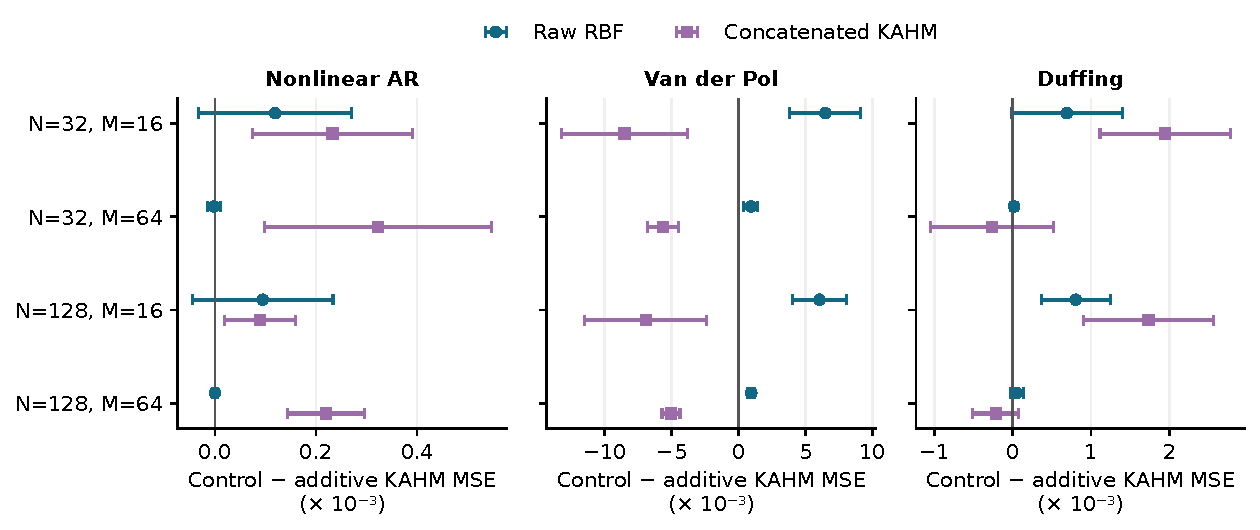
\includegraphics[width=\textwidth]{generated/utility/synthetic_contrasts.pdf}
\caption{Every primary contrast in the new factorial. Points and bars are
mean control-minus-additive-KAHM MSE and the separate 95\% Bonferroni
paired Student intervals over 12 complete repetitions. Positive values
favor additive KAHM. Each panel has its own horizontal range in the same
units; shared data within repetitions pair the $N\times M$ comparisons.
Coverage requires the stated normal approximation and does not imply a
joint claim with earlier interval families.}
\label{fig:utility-contrasts}
\end{figure}

Table~\ref{tab:utility-synthetic} reports every law--data--capacity cell,
including the simpler geometric controls. Figure~\ref{fig:utility-contrasts}
shows all primary intervals. Their lower endpoints exceed zero in
\UtilityRawPositiveContrasts{} of 12 comparisons with raw RBF and
\UtilityConcatPositiveContrasts{} of 12 comparisons with concatenated
KAHM; upper endpoints are below zero in
\UtilityRawNegativeContrasts{} and \UtilityConcatNegativeContrasts{}
comparisons, respectively. An interval spanning zero is unresolved under
this family, not evidence of equality. Complete numeric intervals and
the ridge, persistence, boosting, and fixed-policy controls are retained
in Tables~\ref{tab:utility-intervals}
and~\ref{tab:utility-synthetic-controls}.

The five resolved gains over raw RBF comprise all four Van der Pol
cells and Duffing at $N=128,M=16$. The six resolved gains over
concatenated KAHM comprise all four autoregression cells and both
16-landmark Duffing cells. Conversely, concatenated KAHM beats the
additive construction in all four Van der Pol cells. The mean gain over
raw RBF on Van der Pol is larger at 16 than at 64 landmarks for each
training size, consistent with the correction exploiting structure left
by a limited raw decoder; this is a descriptive capacity pattern, not
a tested interaction or a universal law of model size.

KAHM-specific benefit is not established by these raw-baseline contrasts.
At least one simpler additive control has lower mean error in every
Van der Pol and Duffing cell. Additive KAHM has the lowest mean among
the three additive geometries in the four autoregression cells, but
its raw-baseline intervals there remain unresolved. The fixed boosting
control has the lowest mean among all standalone methods in three
Van der Pol cells; concatenated KAHM is lowest at $N=32,M=64$.
Thus the zero-correction construction preserves a valuable forecast
option without making its ridge correction the best way to use KAHM
geometry. Neither these means nor equal raw landmark budgets establish
equal computational cost or a geometry-specific population advantage.

\subsection{Archive-source utility, selection, and cost}
\label{sec:utility-archive-results}

\paragraph{Fit feasibility is part of the result.}
All 144 synthetic configurations complete. On the archive roster, 22 of
24 configurations complete every procedure. The two capacities for Car
Parts series T1324 each have 23 training histories but only seven distinct
histories. The declared eight-group bank produces fewer nonempty groups
than requested, and the unchanged implementation raises an error rather
than silently dropping a group. Concatenated KAHM and all three additive
geometries fail on both configurations, producing eight failed model fits.
Both declared policies also fail because their required correction
candidate is unavailable. Raw ridge, raw RBF, naive, and boosting forecasts
remain available on all 24 configurations. This is a shared bank-fitting
failure; it does not isolate the KAHM kernel as its cause. No model was
refitted under a changed configuration and no series was replaced.

Consequently, the full-roster KAHM and policy mean losses are undefined.
The reporting amendment retains those failures and adds an explicitly
post-hoc matched-success diagnostic on the 22 configurations where every
procedure completes. This subset has 11 series: three each from Weather,
Solar, and COVID, and two from Car Parts. Sources retain equal weight,
with the remaining Car Parts series now sharing that source's weight.
This comparison conditions on successful fitting and changes the
prespecified roster; it is not the original full-roster estimand or a new
confirmatory transfer result. All-24 baseline outcomes remain visible.

% Generated from the audited forecasting-utility extension; no model fitting.
\begin{table}[!htbp]
\centering\small\setlength{\tabcolsep}{4pt}
\caption{New archive-source coverage and losses. Full-roster scaled MSE uses all 24 configurations and is undefined (dash) for procedures with failed fits. Matched loss and wall seconds use only the post-hoc 22-configuration common-support diagnostic (11 series, including two Car Parts series), with equal source weights. Pipeline costs include all required searches, validation, selected refit, prediction, and serialization. Policy costs are unions of measured required components, including rejected corrections; they are not separately timed full policy executions. Conditioning on success does not complete the prespecified full-roster evaluation.}
\label{tab:utility-archive}
\begin{tabular}{lrrrr}
\toprule
Procedure & Outputs & Full-roster MSE & Matched MSE & Matched seconds \\
\midrule
Raw ridge & 24/24 & 1.2848 & 0.8466 & 0.0015 \\
Raw RBF & 24/24 & 9.6633 & 9.1730 & 0.0037 \\
Concatenated KAHM & 22/24 & \textemdash & 1.2111 & 0.0691 \\
Additive KAHM & 22/24 & \textemdash & 9.1443 & 0.0498 \\
Additive affine & 22/24 & \textemdash & 9.3312 & 0.0369 \\
Additive locality & 22/24 & \textemdash & 9.5624 & 0.0379 \\
Persistence / seasonal naive & 24/24 & 1.5720 & 1.2062 & 0.0012 \\
Histogram gradient boosting & 24/24 & 10.7552 & 10.3174 & 0.6380 \\
KAHM 5\% rule & 22/24 & \textemdash & 9.2460 & 0.0467 \\
All-geometry 5\% rule & 22/24 & \textemdash & 9.2624 & 0.0869 \\
\bottomrule
\end{tabular}
\end{table}


Table~\ref{tab:utility-archive} reports coverage, full-roster losses where
defined, and the separate matched-success diagnostic. Source-specific
losses, leave-one-source-out summaries, actual decoder dimensions, and
all selected mixing weights appear in Appendix~\ref{app:utility-results}.
Among the 22 completed archive comparisons, the KAHM policy adopts a
correction on \UtilityKAHMAdoptions{} configurations and the all-geometry
policy on \UtilityGeometryAdoptions{}. Their decisions use only validation
outcomes. Their matched-success costs include searching corrections even
when the selected test forecast is the raw baseline, but do not redefine
the two failed policy evaluations as successful raw decisions.

On the matched-success diagnostic, raw RBF, concatenated KAHM, and
additive KAHM have scaled MSEs \UtilityRawLoss{}, \UtilityConcatLoss{},
and \UtilityKAHMLoss{}, respectively. The additive improvement over
raw RBF is only \UtilityKAHMGainPercent\% at
\UtilityKAHMCostRatio{} times its measured model-pipeline wall cost.
Raw ridge is both more accurate, at \UtilityRidgeLoss{}, and cheaper,
at \UtilityRidgeCostRatio{} times the raw RBF cost. Concatenated KAHM
substantially improves this weak raw RBF comparator on the diagnostic
subset, but remains worse than raw ridge and has undefined full-roster
loss because of the two failed fits. This is why utility must be judged
against credible simpler alternatives as well as a matched architectural
baseline.

The KAHM 5\% rule has matched-success loss \UtilityPolicyLoss{} at
\UtilityPolicyCostRatio{} times raw RBF's model-pipeline cost; the
all-geometry rule has loss \UtilityGeometryPolicyLoss{} at
\UtilityGeometryPolicyCostRatio{} times its cost. Neither improves
aggregate error on that subset. Positive validation gains therefore do
not establish beneficial test corrections after the pretest refit.

The source detail explains the small additive KAHM aggregate change:
COVID is its only improving source mean, Solar is unchanged, and Weather
and Car Parts worsen. Excluding COVID reverses the aggregate direction
(Table~\ref{tab:utility-leave-one}); this is sensitivity of the same
diagnostic, not additional evidence. The saved-prediction decomposition
likewise has KAHM alignment exceeding correction energy only on COVID,
zero correction on Solar, and negative net gains on the other two sources
(Table~\ref{tab:utility-residual}). The identity verifies how the realized
corrections change squared error without estimating the oracle residual
structure or rescuing the incomplete full-roster evaluation.

\section{Shared proxy-metric geometry and donor residuals}
\label{sec:target-geometry}

The additive experiment leaves two methodological questions open: whether
residuals from models that exclude their query observations improve
correction fitting, and whether a supervised input metric improves KAHM
forecasts. We study these factors with a raw ridge baseline and equally
trained geometric controls. The protocol, input roster, implementation,
and numerical dependencies were archived before full evaluation. The
design uses earlier findings but evaluates additional simulation draws
and four additional source collections.

\subsection{Baseline, residual targets, and matched procedures}
\label{sec:target-procedures}

The base $f_0$ is a raw-history ridge predictor, with its penalty selected
on a separate validation segment. Four gates use the same partition and
reference-selection rules: KAHM reconstruction, affine reconstruction,
locality-aware affine, and a center-distance RBF gate. All retain the
affinity-gated principal coordinates of Equation~\eqref{c:eq:local}.
The RBF-local control therefore describes local affine experts; it is
distinct from the raw Nystr\"om predictor. Requested banks contain
$2,4,8$ groups, rank two, at most 24 references per group and 512 fitting
histories. KAHM queries use the log-shifted Gaussian evaluation in
Section~\ref{c:sec:numerical}.

For each gate we fit three procedures: an identity metric with in-sample
residuals, an identity metric with out-of-fold (OOF) donor residuals, and a
learned metric with those same OOF residuals. The geometry is fitted on the training histories, subject to the
512-history cap. All three correction heads use exactly the same eligible rows,
so the natural-data OOF procedure does not gain a different correction
sample simply by excluding its initial donor prefix. For gate family $g$, let $\Gamma_g(x)$ denote its local feature
vector and let $q_g$ be the fitted residual correction, including
column standardization and a ridge readout. Its output has $H$
coordinates, one for each forecast offset. The forecast is
\[
 \widehat f_g(x)=f_0(x)+\gamma q_g\bigl(\Gamma_g(x)\bigr),
 \qquad \gamma\in\{0,\tfrac14,\tfrac12,1\}.
\]
The baseline and correction penalties use the same seven-value grid
$\{10^{-4},10^{-3},10^{-2},10^{-1},1,10,100\}$. The base is selected
first and held fixed. The candidate set contains zero correction and 21 positive
penalty--weight combinations. Validation chooses a nonzero correction
only when its error is strictly smaller than the baseline error;
subsequent ties retain the earlier candidate in the fixed grid order. The synthetic and archive evaluations retain their selected training-only fits,
without a pretest refit. The zero correction makes the baseline available during selection,
but validation selection does not guarantee improved test error.

Synthetic donors exclude complete independent episodes in four folds.
Natural-series donors use three forward blocks following an initial 40\%
of training origins; every donor target must have been available at the
first forecast origin of its query block. A donor selects its own ridge
penalty using an inner split of its own available data. The final base's
outer-validation choice never feeds backward into donor fitting.
Appendix~\ref{app:target-protocol} gives the boundary and small-sample
rules. Episode exclusion exploits independent synthetic trajectories, whereas
the forward-block construction respects target availability within a
natural series. The appropriate cross-validation design depends on
the forecasting assumptions \citep{Bergmeir2018CV}.

\paragraph{Residuals from different baselines.}
Condition on the fitted representation $\Gamma$, final baseline
$f_0$, and donor baseline $f_d$. Let $(X,Y)$ be a fresh evaluation
pair with $Y\in\R^H$, and write $Z=\Gamma(X)$. All expectations
in this paragraph refer to that evaluation distribution. Define
\[
 m_0(Z)=\E[Y-f_0(X)\mid Z],\qquad
 b_d(Z)=\E[f_0(X)-f_d(X)\mid Z].
\]
The correction minimizing the donor's population residual risk is
$q_d(Z)=m_0(Z)+b_d(Z)$. Assuming $Y$, $f_0(X)$, and $f_d(X)$ have
finite second moments, define $R_H(f)=H^{-1}\E\|Y-f(X)\|_2^2$. Then
\begin{equation}
 R_H(f_0)-R_H(f_0+q_d\circ\Gamma)
 =\frac1H\E\|m_0(Z)\|_2^2-\frac1H\E\|b_d(Z)\|_2^2.
 \label{eq:target-donor-transport}
\end{equation}
This elementary projection identity, proved with its fitted-correction
extension in Appendix~\ref{app:target-transport}, explains why donor
exclusion alone does not establish improvement of a different final
predictor. Chronological folds need not share the same distribution. Our recorded
donor/final disagreement on correction-training rows is a descriptive
diagnostic, not an estimate of either oracle term in
Equation~\eqref{eq:target-donor-transport}.

\subsection{A residual-supervised metric shared across geometries}
\label{sec:target-metric}

We learn a positive diagonal input metric through a Gaussian
kernel-regression proxy, following the supervised metric-learning
principle of \citet{Weinberger2007Metric}. Let $z_i\in\R^d$ denote a training-standardized history, with
$d=L$ equal to the history length, and let $s_i\in\R^H$ denote its donor residual vector,
centered by output and divided by one pooled residual standard deviation.
The shared scalar division preserves relative original-unit horizon
weights. On at most 256 training correction rows, set
\begin{align}
 d_\theta^2(z_i,z_j)&=\sum_{k=1}^{d}e^{\theta_k}(z_{ik}-z_{jk})^2,
 &p_{ij}(\theta)&=
 \frac{\exp\{-d_\theta^2(z_i,z_j)/(2\sigma^2)\}}
      {\sum_{l\in\mathcal A_i}\exp\{-d_\theta^2(z_i,z_l)/(2\sigma^2)\}},
 \quad j\in\mathcal A_i,\label{eq:target-metric-weights}\\
 \mathcal J(\eta)&=
 \frac{1}{|\mathcal I|H}\sum_{i\in\mathcal I}
 \left\|s_i-\sum_{j\in\mathcal A_i}p_{ij}(\theta)s_j\right\|_2^2
 +\frac{0.05}{d}\|\theta\|_2^2,
 &\theta&=\eta-\overline\eta\mathbf1.
 \label{eq:target-metric-objective}
\end{align}
The admissible donor-index set $\mathcal A_i$ excludes the query's episode for synthetic
data, or origins separated from the query by at most $L+H$ steps for natural
data. The set $\mathcal I$ contains queries with at least one admissible
donor. The vector $\eta\in\R^d$ contains free optimization parameters,
$\overline\eta=d^{-1}\sum_k\eta_k$, and $\theta$ is its centered
version. Thus $e^{\theta_k}$ is the metric weight of input coordinate $k$. The bandwidth $\sigma^2$ is the identity-metric
median positive admissible squared distance and remains fixed during
optimization. The box $|\eta_k|\leq\log(16)/2$ bounds the ratio between
the largest and smallest metric weights by 16; their geometric mean is
one. Indeed, $\theta_k-\theta_l=\eta_k-\eta_l$ is at most
$\log16$, and $\sum_k\theta_k=0$. The box constraint applies
to $\eta$; the centered coordinates $\theta_k$ need not lie in
the same interval.

The limited-memory bound-constrained quasi-Newton optimizer L-BFGS-B
uses the analytic gradient and at most 40 iterations.
Identity is the declared fallback for an unavailable or nonfinite
objective, constant residuals, or a worse final iterate. Finite improved
iterates at the iteration limit are retained with their convergence
status. No validation or test outcomes enter this optimization. Natural
metric donors may be earlier or later within the training period: this
is offline supervised fitting, separate from the forward construction
of baseline residuals.

The same learned weights are applied \emph{after} input standardization
for all four geometric gates; subsequent partitioning and local models
are refitted under that metric. This is a supervised kernel proxy
transferred to KAHM and its controls, not end-to-end minimization of
KAHM forecasting loss. Its training objective may decrease without
improving the final decoder. The comparison with equally trained local
controls tests whether any benefit is specific to the KAHM reconstruction.

\subsection{Declared evaluation and complete accounting}
\label{sec:target-evaluation}

Twelve independent repetitions of each of the nonlinear AR, Van der
Pol, and Duffing laws give 36 synthetic tasks. Each uses 128 training,
64 validation and 128 test episodes, history 12, direct offsets $1,4,12$
and the observation models in Appendix~\ref{c:app:methods}. Six prespecified comparisons per
law isolate learned-OOF KAHM versus ridge, learned versus identity
metric for OOF KAHM, OOF versus in-sample targets at the identity metric,
and learned-OOF KAHM versus each of the three equally trained geometric
controls. All 18 comparisons receive two-sided Bonferroni-adjusted
paired Student intervals over the 12 complete repetition differences.
Their coverage uses a normal approximation; origins and horizons do not
increase the replication count. These fresh simulations supply new
stochastic evidence on known laws, not new-domain confirmation.

Four additional Monash collections \citep{Godahewa2021Monash} provide
Australian state electricity demand, Bitcoin activity indicators,
Melbourne pedestrian counts, and KDD2018 air quality. Three series per
collection are selected using training-prefix eligibility and fixed hash ordering. The 12-series roster and split rules are specified in
Appendix~\ref{app:target-protocol}. These collections were not used in the earlier evaluations, although
some application domains overlap. They are not a
random sample of future forecasting applications. Natural results use
equal weights for series within source and for the four sources;
overlapping windows do not create independent source replications.

The 16 procedures comprise the 12 geometric corrections, ridge,
raw Nystr\"om-plus-linear regression, naive prediction, and a jointly
fitted raw-plus-KAHM ridge readout. The last is a secondary architecture
control and differs from the earlier concatenated Nystr\"om procedure.
The protocol reduces group counts when local training histories are
insufficiently distinct and uses predefined ridge fallbacks for
unavailable correction fits. Fewer than eight eligible correction rows
or a failed secondary joint head invokes a fallback for the affected
arms while retaining the available baselines. These fallback rules belong to this experiment; the additive study in
Section~\ref{sec:utility-extension} used a different failure policy.
Full-roster results remain unavailable if a primary baseline or required
task output is missing.

Warm pipeline cost charges each method for its complete required
baseline, donor, metric, bank, head-selection and serialization work,
including rejected candidates and fallbacks. Shared components are
charged once per standalone procedure. These are measured component
sums on one host, not repeated end-to-end deployment timings or minimum
possible complexity. Tables~\ref{tab:target-synthetic-main}
and~\ref{tab:target-archive-main} report the declared comparisons;
Appendix~\ref{app:target-results} retains all contrasts, source-level
results, fitting diagnostics, and resource records.

\subsection{Results: predictive gains and their attribution}
\label{sec:target-results}

All 48 tasks and 768 method--task forecast outputs completed, without
fallbacks. Learned-OOF KAHM reduces mean synthetic MSE relative to ridge
by 11.18\% on nonlinear AR, 53.26\% on Van der Pol, and 19.44\% on
Duffing. All three adjusted paired intervals favor the correction.
However, the three learned-versus-identity metric intervals and the
three OOF-versus-in-sample target intervals all include zero. These
comparisons do not establish equivalence; they leave the incremental
benefits of the two proposed changes unresolved at the declared
precision. Among nine comparisons with equally trained geometric
controls, none favors KAHM with an interval excluding zero. Five favor
the control: locality and RBF-local on Van der Pol, and all three on
Duffing. The other four remain unresolved. Thus the 18-contrast family
contains three favorable, five unfavorable, and ten unresolved results
for its designated candidates
(Appendix~\ref{app:target-results}). The secondary raw RBF predictor
also has lower mean MSE than learned-OOF KAHM on every law; this mean
ranking has no additional confirmatory interval.

On the four archive collections, learned-OOF KAHM has
source-balanced scaled MSE 1.272128 versus ridge's 1.300458, a
descriptive 2.18\% reduction. Its charged mean pipeline time is
0.1622\,s versus 0.001299\,s for ridge, or $124.9\times$ on this host.
The identity-metric in-sample KAHM procedure achieves a lower loss,
1.264589 (2.76\% below ridge), at $39.3\times$ ridge's time. The
lowest archive mean among the specified procedures is 1.257888 for identity-metric,
in-sample RBF-local correction. Learned-OOF affine and locality also
have lower means than learned-OOF KAHM, at 1.268679 and 1.266922,
respectively. Figure~\ref{fig:target-accuracy-cost} places the modest
archive accuracy changes alongside their measured computational cost;
the added metric stage is not supported as a default improvement by
these results.

Learned-OOF KAHM improves the mean in each of the four collections,
but improves only seven of the 12 individual series, worsens four,
and exactly retains ridge on one through zero correction. Omitting
each collection in turn leaves descriptive aggregate gains of
1.49--3.35\%. This sensitivity check shows that the sign does not
depend on retaining any one collection; it does not expand the
population represented by four selected collections or supply an
independent replication. These results establish improvement
over the selected ridge reference in the stated settings while
leaving a KAHM-specific advantage unsupported. The gains over ridge can also be obtained by simpler geometric
controls under these settings.

% Generated only from audited target-geometry predictions; no fitting.
\begin{table}[!htbp]
\centering\small\setlength{\tabcolsep}{4pt}
\caption{Fresh synthetic repetitions: mean test MSE $\times10^3$ over all 12 independent repetitions per law, with equal episode, origin and horizon weights. Every declared procedure is shown. A dash denotes an incomplete full roster; baseline fallbacks retain their actual forecasts. Differences are assessed by the 18 prespecified paired intervals in Table~\ref{tab:target-synthetic-intervals}, not by ranking these means.}
\label{tab:target-synthetic-main}
\begin{tabular}{lrrr}
\toprule
Procedure & Nonlinear AR & Van der Pol & Duffing \\
\midrule
Raw ridge & 5.057 & 44.140 & 6.916 \\
Raw RBF & 4.442 & 8.316 & 4.172 \\
Persistence / seasonal naive & 8.549 & 293.407 & 37.977 \\
Joint raw + KAHM & 4.465 & 17.009 & 5.277 \\
Fixed, IS KAHM & 4.478 & 21.380 & 5.468 \\
Fixed, IS Affine & 4.470 & 18.986 & 4.706 \\
Fixed, IS Locality & 4.503 & 13.699 & 4.508 \\
Fixed, IS RBF local & 4.427 & 15.987 & 5.318 \\
Fixed, OOF KAHM & 4.481 & 21.383 & 5.469 \\
Fixed, OOF Affine & 4.473 & 18.983 & 4.721 \\
Fixed, OOF Locality & 4.506 & 13.700 & 4.512 \\
Fixed, OOF RBF local & 4.431 & 15.988 & 5.321 \\
Learned, OOF KAHM & 4.492 & 20.629 & 5.572 \\
Learned, OOF Affine & 4.460 & 18.879 & 4.736 \\
Learned, OOF Locality & 4.530 & 13.968 & 4.536 \\
Learned, OOF RBF local & 4.408 & 15.460 & 5.328 \\
\bottomrule
\end{tabular}
\end{table}

% Generated only from audited target-geometry predictions; no fitting.
\begin{table}[!htbp]
\centering\small\setlength{\tabcolsep}{4pt}
\caption{Natural-data forecasting results: equal-collection means of equal-series scaled MSE and charged standalone wall seconds, covering four collections and three series per collection. Scaling uses training-only seasonal-difference MSE (first-difference fallback). IS denotes in-sample residuals and OOF denotes out-of-fold residuals. Change is relative to raw ridge; negative is favorable. Fallbacks predict raw ridge and retain attempted computation. Missing tasks make the affected full-roster means undefined. These are descriptive results, with no population confidence intervals or independence claims for adjacent origins.}
\label{tab:target-archive-main}
\begin{tabular}{lrrrrr}
\toprule
Procedure & Outputs & Scaled MSE & Change (\%) & Seconds & Fallbacks \\
\midrule
Raw ridge & 12/12 & 1.3005 & 0.00 & 0.001 & 0 \\
Raw RBF & 12/12 & 1.9483 & 49.82 & 0.005 & 0 \\
Persistence / seasonal naive & 12/12 & 1.8476 & 42.07 & 0.004 & 0 \\
Joint raw + KAHM & 12/12 & 1.4530 & 11.73 & 0.058 & 0 \\
Fixed, IS KAHM & 12/12 & 1.2646 & -2.76 & 0.051 & 0 \\
Fixed, IS Affine & 12/12 & 1.2584 & -3.24 & 0.029 & 0 \\
Fixed, IS Locality & 12/12 & 1.2635 & -2.84 & 0.028 & 0 \\
Fixed, IS RBF local & 12/12 & 1.2579 & -3.27 & 0.027 & 0 \\
Fixed, OOF KAHM & 12/12 & 1.2767 & -1.83 & 0.056 & 0 \\
Fixed, OOF Affine & 12/12 & 1.2731 & -2.11 & 0.034 & 0 \\
Fixed, OOF Locality & 12/12 & 1.2735 & -2.07 & 0.032 & 0 \\
Fixed, OOF RBF local & 12/12 & 1.2746 & -1.99 & 0.031 & 0 \\
Learned, OOF KAHM & 12/12 & 1.2721 & -2.18 & 0.162 & 0 \\
Learned, OOF Affine & 12/12 & 1.2687 & -2.44 & 0.142 & 0 \\
Learned, OOF Locality & 12/12 & 1.2669 & -2.58 & 0.141 & 0 \\
Learned, OOF RBF local & 12/12 & 1.2848 & -1.20 & 0.139 & 0 \\
\bottomrule
\end{tabular}
\end{table}

\begin{figure}[!htbp]
\centering
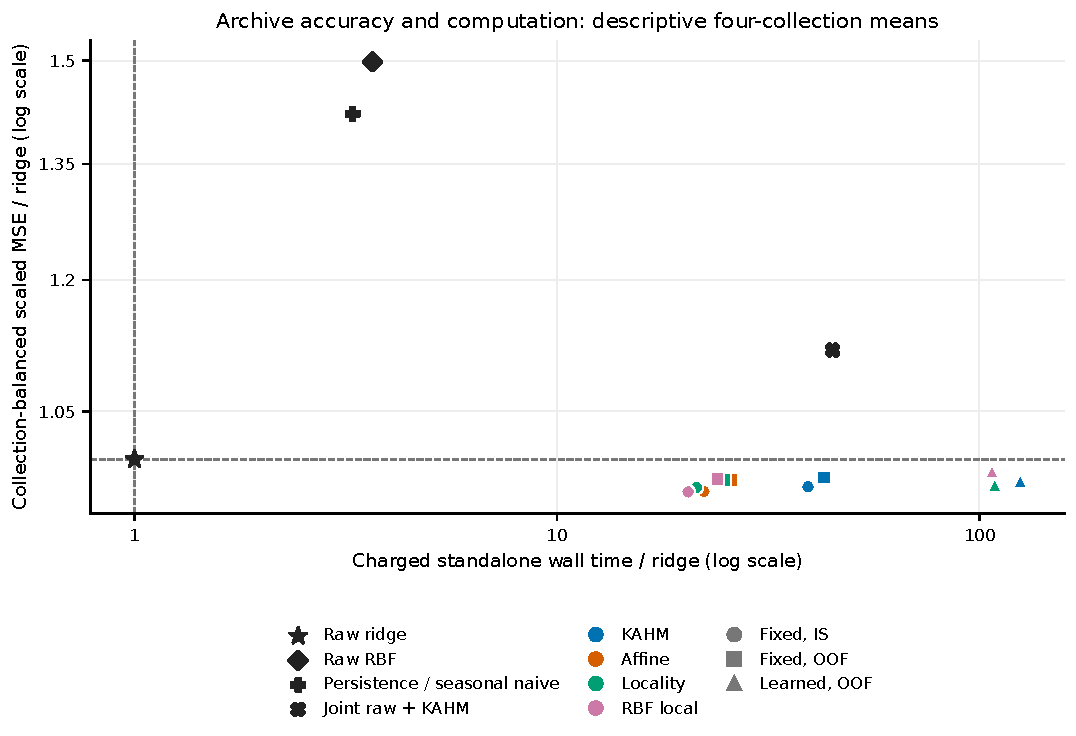
\includegraphics[width=0.96\linewidth]{generated/target_geometry/archive_accuracy_cost.pdf}
\caption{Accuracy and charged computation on the four archive
collections. Both axes divide the source-balanced method mean by the
corresponding ridge mean and use logarithmic scales. Lower loss and
lower time are preferable. Circles, squares, and triangles distinguish
identity/in-sample, identity/OOF, and learned/OOF procedures. Times
charge the complete required components of each method, including
selection; they are descriptive measurements from one host. The plot
shows all 16 procedures without implying uncertainty intervals or a
population-wide ranking.}
\label{fig:target-accuracy-cost}
\end{figure}
\FloatBarrier

\section{Interpretation and limitations}\label{sec:discussion}
\paragraph{What the combined evidence supports.}
The branch intervention shows how accurate reconstruction can coexist
with a poor predictive code, and how explicit position or a locality-aware
score can repair it. The fresh synthetic study shows that representation
and finite decoder must be evaluated jointly: KAHM helps on a declared
law while other controls win on others. The separate natural-source study
shows that those controlled gains do not suffice to recommend its tested
augmentation broadly. These results concern different procedures and
populations; neither the natural failures erase the controlled effects
nor the controlled effects override the natural failures.
The later paired scaling check leaves the natural aggregate ranking intact
under the specified unclipped min--max alternative. It strengthens that
bounded comparison without extending it to every preprocessing choice or
future source population.
The main controlled local-coordinate comparisons retain their mean ordering,
although Duffing's KAHM error
changes appreciably. Robustness of a ranking within these two fixed scaler
arms is a narrower statement than invariance of the representation or loss.

The additive extension adds a distinct qualification. Preserving the raw
forecast makes a zero correction feasible for a successfully fitted model,
but does not establish that the correction is useful, that KAHM is the
best correction geometry, or that the procedure completes every fit.
The synthetic factorial finds gains against raw RBF in selected cells,
while concatenated KAHM, simpler additive controls, or boosting are better
in others. The two archive fitting failures prevent a full-roster
geometric loss comparison. On the explicitly post-hoc matched-success
diagnostic, raw ridge is substantially more accurate and cheaper than
the geometric alternatives, and neither frozen 5\% policy improves the
raw RBF aggregate. An architectural safeguard and a validation margin
are therefore useful design choices to evaluate, not adoption guarantees.

The target-geometry study adds evidence for a more specific time-series
role. KAHM local features can correct a ridge forecast on all three known
synthetic laws and modestly improve the new archive aggregate. Those
improvements are properties of the complete procedures. The simultaneous
comparisons do not establish a benefit from switching to donor residuals
or learning the shared proxy metric, and five favor simpler matched
geometries. Raw RBF also has lower mean error on each synthetic law in
this experiment. On the archive, fixed-metric in-sample KAHM is both more
accurate and cheaper than learned-metric OOF KAHM. Thus the successful
ridge correction does not identify supervised metric learning, donor
exclusion, or the KAHM gate as its unique source.

For evaluating another reconstruction-based feature map, the resulting
questions are concrete. Does fitting complete on the declared inputs?
Does the code retain target-relevant position?
Does a simpler locality or affine control recover the same benefit?
Does the comparison persist with a raw-input control and an explicitly
specified decoder? Does it survive complete selection costs and evaluation
on reserved original sources? The present experiments demonstrate why
each check can change the interpretation. They do not provide an automatic
test for choosing a representation.

\paragraph{Limits of the benefit diagnostic.}
The four tested rules use a small set of descriptors and one reduced-capacity
probe. In particular, the descriptors omit downstream landmark count;
when the training cap is nonbinding, different capacities can receive
identical descriptors. History and horizon also change together.
Moreover, selecting by the sign of expected log loss ratio need not minimize
expected scaled MSE: heterogeneous loss magnitudes matter even when each
realized log ratio has the same sign as the corresponding raw-minus-KAHM
loss difference. We therefore report the
actual decision losses and costs as well as prediction error. The failed
geometric increment motivates the separately frozen additive extension
and new archive sources in Section~\ref{sec:utility-extension}. It does
not justify retuning a diagnostic on the already inspected confirmation
outcomes and reporting them as a new test.

\paragraph{Limits of data, inference, and computation.}
The eight natural source families were selected for diversity and feasibility,
not sampled randomly from future applications. Four families per phase
support bounded descriptive comparisons; related windows, settings, and
seeds do not enlarge that number. Longer Hospital and Traffic regimes
have only 21 and 29 initial training windows, and one NN5 regime retains
seven test origins. Missing-window exclusion defines an available-window
estimand. FRED-MD is a fixed retrospective snapshot whose upstream
transformations and release-time revisions are not fully audited here.

The original natural candidates are local univariate forecasters with two capacity
settings and finite grids. The study is not a comprehensive neural or
pretrained forecasting benchmark. The MLP reaches its iteration cap in
68 of 80 selected confirmation refits; all such fits and warnings remain
reported. Equal landmark counts do not imply equal effective capacities,
and that study's two settings jointly vary sample and model-size caps. CPU timings
are implementation-specific, include material bookkeeping, and expose
imports/launch separately. Process high-water RSS includes interpreter and
input storage and cannot resolve incremental memory use. Model bytes,
training memory, energy, and financial cost are different quantities.

The controlled Student intervals rely on their stated paired-difference
assumptions. The original 29- and 12-contrast families and the new
24-contrast additive extension and 18-contrast target-geometry study
retain separate coverage claims, without a joint
95\% guarantee across the entire paper.
The branch reflection and saved-bank conditioning checks are descriptive;
they supply neither a population Lipschitz bound nor a distribution-free
KAHM performance certificate. Replaying fixed seeds and reconstructing
saved losses verifies computation without producing new source evidence.

The scaling analysis compares two fixed preprocessing choices on those same
observations. It does not test clipping, all alternative scalers, local-only
natural models, or a new scaler-selection rule. Near-equal natural aggregate
errors do not prove statistical equivalence or scale invariance. Conversely,
an observed controlled change describes the complete refitted pipeline:
partitioning, truncated directions, reference-energy regularization, gates,
and finite decoder geometry can all change together. Further component
attribution or a newly chosen procedure would require another specified study
and fresh reserved evidence for a new transfer claim.

\paragraph{Scope of the additive extension.}
The new factorial separates the number of training episodes from the raw
decoder's requested landmark count. It holds the declared geometric bank
configuration and ridge-correction class fixed; it does not identify an
optimal KAHM rank, reference count, or decoder family. More training data
can also change the fitted partitions and residual targets. The correction
learns in-sample residuals of a selected raw predictor, so insufficient
residual structure, overfitting in either stage, the coarse penalty and
mixing grids, and finite validation data can all affect its usefulness.
A favorable comparison identifies a useful complete procedure under that
protocol; an adverse comparison does not establish that every KAHM decoder
or every residual-fitting construction must fail.

The new archive evaluation contributes four selected collections, three
series per collection, two requested capacities, and one fitting seed.
Solar Weekly has simulation provenance. This is a bounded extension of
source coverage, not a representative survey of forecasting domains.
Actual landmark counts and retained kernel ranks can be below their
requested values on short series. The initial chronological validation
rule is applied before a pretest refit, which changes the baseline,
residual targets, and correction together. No positive test guarantee
follows from a 5\% validation margin, an exact zero-correction option,
or a positive alignment computed after observing test outcomes. In fact,
the shared geometric-bank fit fails on both capacities of one Car Parts
series, before a zero-correction choice can be evaluated. Full-roster
geometric and policy mean losses are therefore undefined. The amended
22-configuration comparison is conditional on successful fitting, with
only two Car Parts series, and cannot be presented as completion of the
prespecified full-roster evaluation. The robust fallback and revised grouping rules in
Section~\ref{sec:target-geometry} are changed procedures evaluated
separately; they do not replace these historical failures.

The utility decision is also application-dependent. This study supplies
measured loss--cost pairs and fixed policy outcomes; it does not impose a
deployment latency budget, a memory ceiling, or an exchange rate between
accuracy and resources. Component-sum policy costs expose required shared
work but are not separately timed end-to-end executions. Actual serialized
state is not a lower bound on model storage, and a single execution cannot
resolve small timing differences as precisely as a repeated benchmark.
These limits matter when translating a favorable error comparison into a
claim that additional representation complexity is justified.

\paragraph{Scope of target-trained geometry and donor residuals.}
The latest experiment tests one constrained diagonal metric, one fixed
Gaussian proxy bandwidth, one 256-row metric cap, one regularization
strength and a finite family of readouts. All metric fits converge under
the optimizer's criterion, but the median regularized objective reduction
is small. Convergence and a lower training proxy are not evidence of a
useful forecast geometry. The experiment is not an exhaustive search over
supervised metrics, and it does not train KAHM's reconstruction parameters
directly against forecast error. Its three known laws, four selected
collections, fixed contexts/horizons, and capped training sizes bound the
conclusion. Neither overlapping windows nor multiple gates expand the
number of independent natural collections.

Donor exclusion prevents a predictor from fitting its own query label;
it does not make donor and final-model residual distributions identical.
The elementary identity in Equation~\eqref{eq:target-donor-transport}
conditions on fixed maps under a common evaluation law. Chronological
folds can have different laws and sample sizes, so their observed
prediction disagreement supplies a diagnostic rather than an oracle-risk
certificate. The new comparison also makes no pretest refit, holding the
selected base fixed. This differs materially from the earlier utility
study and avoids attributing all between-study changes to residual honesty.

The archive gain from learned-metric KAHM is 2.18\%, while the charged
standalone procedure costs about 0.162 seconds per task versus 0.00130
seconds for ridge on the recorded host. The ratio of approximately 125
therefore accompanies small absolute times at the tested scale; it is
neither an intrinsic algorithmic constant nor evidence of deployment
infeasibility. Fixed-metric KAHM and simpler controls nevertheless supply
better observed accuracy--cost pairs here. Computation includes the paid
metric, donors and selection, and conservatively retains test bank
transform costs when validation chooses zero correction. It does not
measure peak incremental memory, streaming update latency or optimized
production kernels.

\paragraph{A focused research program for KAHM forecasting.}
The evidence supports studying KAHM as a local representation whose
usefulness depends on target, decoder and resources. A next methodological
step is to train a KAHM gate or reconstruction parameter against a
forecast-specific objective, with horizon-specific or low-rank metrics
as explicit alternatives. Such a study should include the same supervision
and optimization budget for affine, locality and RBF-local controls;
otherwise a gain would confound supervised fitting with the KAHM rule.
This is an untested hypothesis, not a conclusion of the present proxy
experiment. More capacity is justified only by fresh held-out improvement
over those controls and the strongest practical raw-input baseline.

A second direction is efficient updating of useful local structure.
Reference reduction, cached local factorizations and bounded updates
could change the measured cost tradeoff, but no streaming or drift
experiment is reported here. A new chronological protocol should jointly
measure prediction, update latency and memory, with a rule for retiring
or declining an unhelpful correction. Larger independent source coverage
and stronger forecasting baselines would then test transfer. The present
archive outcomes can guide development; they cannot be reused as unseen
confirmation of a newly chosen method.

\section{Conclusion}
KAHM can be studied productively in time-series forecasting as a local
geometric representation with an explicit decoder and baseline. The
controlled intervention identifies when reconstruction scores omit
predictive position; the original finite-decoder study demonstrates
conditional gains. Natural-source and scaling experiments limit their
transfer, and the additive utility study exposes both weak incremental
benefit and fitting failures. These observations remain part of the
scientific record.

The new prospectively frozen study completes all 48 tasks and 768
forecasts, evaluates honestly excluded donor residuals and a shared
supervised metric, and supplies an elementary account of donor-to-final
residual mismatch. Learned-metric KAHM improves ridge on the three
synthetic laws and by 2.18\% on the four-collection archive aggregate.
However, incremental metric and donor-target benefits are unresolved in
the synthetic family, matched local controls win five comparisons, and
fixed-metric KAHM or simpler corrections offer better archive tradeoffs.
These results justify continued investigation of target-relevant local
geometry while leaving a KAHM-specific advantage unestablished.

A defensible forecasting contribution therefore requires more than
reconstruction accuracy or retention of the raw pathway: it must identify
what the geometry adds beyond matched alternatives, show that the gain
survives temporal evaluation, and report the complete resources used to
obtain it. The revised framework and reproducible evidence make those
questions concrete. Direct forecast-trained KAHM geometry and efficient
adaptation remain testable next steps rather than promised improvements.


\section*{Reproducibility and research transparency}
The supplementary source contains the editable manuscript, its generated
tables and figures, and instructions for compiling the PDF. The code and
evidence materials organize each experiment separately. For each study,
they specify the observation or dataset sources, preprocessing, split
roles, model-selection rules, statistical contrasts, and resource
accounting. Machine-readable records include predictions, targets,
selected configurations, warnings, and unsuccessful or unavailable tasks.
Checksums identify the source and data associated with each reported run.
The accompanying reproduction guide distinguishes reconstruction of
reported results from refitting the forecasting models.

For the reconstruction-departure experiment, the prospective local record
contains 239 source, configuration, and input files for all 192 task
suites. All ten procedures finish on every task, yielding 1,920 saved
prediction arrays and 9,584,640 forecast values. The statistical analysis
uses 24 independent repetition aggregates. An analysis program that does
not import the forecasting implementation reconstructs losses and all
six primary contrasts from the predictions. Separately implemented
feature evaluation, ridge prediction, and tree traversal check the saved
selected states, normal equations, window chronology, and selection
rules. Selected-state replay reproduces all 1,920 prediction arrays
exactly in the recorded environment. Discarded hyperparameter candidates
have saved validation scores but not all fitted coefficients; their
selection scores can be checked without claiming an independent refit.

Earlier studies retain their own evidence and verification procedures.
The additive-correction study records 1,344 attempted standalone fits,
including eight failures and four unavailable dependent policy outputs
on two configurations. Its successful-subset natural-data analysis is
identified as post hoc. The target-geometry study retains all 768
forecasts from its 48 tasks. The direct-training study retains all 46
planned tasks, including three with no eligible training-query windows.
The adaptive study retains the original numerical failure and the results
obtained after the documented solver correction. These computational
records support traceability and consistency; they are not external
replications or additional independent observations.

The anonymous saved-forecast supplement contains the numeric predictions
and evaluation targets for all 192 task suites, together with the fitting
targets needed to reconstruct loss normalization. Its standalone program,
\path{verify_saved_forecasts.py}, recomputes the eight numerical analysis
tables and all six primary contrasts, verifies array identities, and checks
that each saved policy forecast equals its recorded selected procedure.
This supplement supports statistical reproduction from saved forecasts;
it does not refit models or recompute feature bounds and resource timings.

\paragraph{Use of AI tools.}
AI tools assisted with protocol development, implementation, numerical and
statistical verification, analysis, and writing. The authors are
responsible for the scientific claims, the accuracy of the evidence,
and the final manuscript.

\bibliography{references}
\bibliographystyle{tmlr}
\appendix
% Supporting theory and exact methods. The main document invokes \appendix.
\section{Supporting Mathematical Statements}\label{c:app:theory}

The statements in this appendix make the interpretation of the experiments
precise. They are elementary supporting results; we do not claim a new
KAHM approximation theorem. All conditional expectations below are understood
up to almost-sure equality. For scalar square-integrable $Y$, write
$m(X)=\E[Y\mid X]$ and
$R_X^{\mathrm{Bayes}}=\E[(Y-m(X))^2]$.
When a representation has been learned from independent training data,
the statements apply conditionally on that fitted representation.

\begin{proposition}[Information retained by a representation]
\label{c:prop:representation-risk}
For a measurable representation $U=\Gamma(X)$,
\[
 R_U^{\mathrm{Bayes}}-R_X^{\mathrm{Bayes}}
 =\E[(m(X)-\E[m(X)\mid U])^2].
\]
For any square-integrable prediction $f(U)$,
\[
 R(f\circ\Gamma)-R_X^{\mathrm{Bayes}}
 =\|m-f\circ\Gamma\|_{L^2}^2.
\]
\end{proposition}
\begin{proof}
Write $Y-f(U)=(Y-m(X))+(m(X)-f(U))$.
The cross term has expectation zero after conditioning on $X$.
Minimizing the second term over $U$-measurable predictions gives the
conditional expectation $\E[m(X)\mid U]$.
\end{proof}

\begin{proposition}[Restoring the outer score normalizer]
\label{c:prop:normalizer-inverse}
Let $T_1,\ldots,T_C\in[0,1]$, $\omega>0$, and $\tau>0$. Define
\[
 \ell_c=\omega\log(1-T_c+\tau),\qquad
 z=\log\sum_{j=1}^{C}\exp(\ell_j),\qquad
 \phi_c=\exp(\ell_c-z).
\]
Then $T$ and $(\phi,z)$ generate the same information in exact arithmetic,
and
\[
 T_c=1+\tau-\exp\{(\log\phi_c+z)/\omega\}.
\]
For multiple separately normalized blocks, one $z$ is required per block.
\end{proposition}
\begin{proof}
Strict positivity of $1-T_c+\tau$ implies $\phi_c>0$.
Hence $\log\phi_c+z=\ell_c$, which gives the inverse.
Both directions are measurable. Applying this argument to each block
gives the multiple-block statement.
\end{proof}

If scores are clipped before normalization, the inverse restores the
clipped scores. It does not restore discarded reconstruction vectors or
guarantee equal finite-head performance. In particular, the inverse is
nonlinear, so affine function classes on $T$ and on $(\phi,z)$ need not
coincide. This proposition concerns the outer association normalizer,
not the signed denominator in the KAHM reconstruction.

\begin{proposition}[A sufficient condition for an injective local code]
\label{c:prop:local-injectivity}
Fix a fitted bank with bases $P_c$ and centers $\mu_c$. Suppose its gates
are measurable and strictly positive, and let $A$ be the matrix obtained by vertically
stacking the matrices $P_c^\top$. If $A$ has full column rank $d$, then
\[
 z\longmapsto
 \left[\phi(z),\{\phi_c(z)P_c^\top(z-\mu_c)\}_c\right]
\]
is injective. In particular, this code and $z$ generate the same
information, and their Bayes risks agree for every square-integrable
target.
\end{proposition}
\begin{proof}
The code contains both $\phi_c(z)>0$ and its product with
$P_c^\top(z-\mu_c)$. Division and addition of the fixed vector
$P_c^\top\mu_c$ recover $P_c^\top z$ for every $c$. Stacking these
vectors gives $Az$. Full column rank gives the measurable inverse
$z=(A^\top A)^{-1}A^\top(Az)$. Conversely, the code is a measurable
function of $z$, so the generated information and Bayes risks agree.
\end{proof}

The gates in Equation~\eqref{c:eq:phi} are strictly positive in exact
arithmetic because $\tau>0$. The rank assumption is a sufficient
condition, not a necessary one: when $A$ is rank deficient, the gates
themselves may retain additional information. It must be checked for
each fitted bank. Very small gates and an ill-conditioned $A$ can make
the displayed inverse numerically unstable, and its existence does not
make it accessible to every finite decoder or fitting procedure.

\begin{proposition}[A score symmetry and its prediction consequence]
\label{c:prop:exact-symmetry}
Let $Q$ be orthogonal on a preprocessed input space. Suppose that each
group's reconstruction obeys $r_c(Qx)=Qr_c(x)$ and that $Q$ preserves
group identities. The radial--angular score in Section~\ref{c:sec:method},
its block affinities, and the block log normalizer are invariant under $Q$.

For the branch law in Equation~\eqref{c:eq:branch}, let
$Q(x_1,x_2)=(-x_1,x_2)$. Any representation $U=\Gamma(X)$ satisfying
$\Gamma(QX)=\Gamma(X)$ almost surely has
\[
 R_U^{\mathrm{Bayes}}
 =\frac{1}{300}+\lambda
  +(1-\lambda)\E[(S-\E[S\mid U])^2].
\]
Consequently $R_U^{\mathrm{Bayes}}\geq 1/300+\lambda$, with equality
when $U$ determines $S$.
\end{proposition}
\begin{proof}
Orthogonality preserves norms and inner products, including the zero-norm
convention for the angle. Equivariance therefore preserves each radial
and angular discrepancy, hence its combined score. Block normalization
and its log normalizer are deterministic functions of those scores.

For the branch law, replacing $T$ by $-T$ leaves the joint distribution
of $(S,T)$ unchanged and leaves $U$ unchanged. Thus $\E[T\mid U]=0$.
Also $S$ is even under this reflection, whereas $T$ is odd. It follows
that $\E[(S-\E[S\mid U])T]=0$. Expanding the square in
Proposition~\ref{c:prop:representation-risk}, using
$\E[T^2]=1/3$ and $\Var(\epsilon)=1/300$, yields the displayed identity.
\end{proof}

The first assertion also holds when $Q$ permutes reconstructors within a
group whose score is their minimum. Permuting distinct groups, however,
can permute the affinity coordinates rather than leaving the representation
unchanged. Nor does a raw-input reflection necessarily commute with a
training-fitted scaler. Finite learned partitions and reference sets need
not satisfy the proposition's assumptions. The measured near-invariance
of one learned code is therefore a diagnostic, not a proof that its
Bayes risk equals the exact-symmetry lower bound. Tiny nonzero differences
could in principle be used by an unrestricted decoder.

\begin{proposition}[Approximate symmetry under a decoder budget]
\label{c:prop:approx-symmetry}
Let $Q$ be a measurable, distribution-preserving involution on the input
space: $Q^2X=X$ almost surely and $QX$ has the law of $X$.
Let $d_U$ be a measurable pseudometric on the representation space and
$g$ be $\kappa$-Lipschitz for this pseudometric. Assume
$m,g\circ\Gamma\in L^2$ and
\[
 \delta_\Gamma^2
 =\E[d_U(\Gamma(X),\Gamma(QX))^2]<\infty.
\]
With $m_o=(m-m\circ Q)/2$,
\[
 R(g\circ\Gamma)-R_X^{\mathrm{Bayes}}
 \geq (\|m_o\|_{L^2}-\kappa\delta_\Gamma/2)_+^2.
\]
For the branch law, $\|m_o\|_{L^2}=\sqrt\lambda$.
\end{proposition}
\begin{proof}
The operator $Vh=h\circ Q$ is an isometric involution on $L^2(P_X)$.
The even and odd components $h_e=(h+Vh)/2$ and $h_o=(h-Vh)/2$
are orthogonal. In particular, with $f=g\circ\Gamma$,
\[
 \|m-f\|_{L^2}^2
 =\|m_e-f_e\|_{L^2}^2+\|m_o-f_o\|_{L^2}^2
 \geq\|m_o-f_o\|_{L^2}^2.
\]
The Lipschitz condition gives
$|f_o(X)|\leq\kappa d_U(\Gamma(X),\Gamma(QX))/2$, so
$\|f_o\|_{L^2}\leq\kappa\delta_\Gamma/2$.
Apply the reverse triangle inequality and
Proposition~\ref{c:prop:representation-risk}.
For the branch law, $m_o(X)=\sqrt{3\lambda}\,T$ and
$\E[T^2]=1/3$.
\end{proof}

An empirical reflection distance is not automatically a population upper
bound for $\delta_\Gamma$. A valid numerical lower bound obtained from
this proposition would need uncertainty control in that direction and a
verified decoder Lipschitz constant for the same metric. Neither is
asserted for the experiment's unconstrained diagnostic heads.

\begin{proposition}[Reconstruction through the predictor's representation]
\label{c:prop:reconstruction-bridge}
Suppose a version of $m$ is $L$-Lipschitz on a domain containing $X$ and
$h(U)$ almost surely, and
$\E\|X-h(U)\|_2^2\leq\varepsilon_{\mathrm{rec}}^2$.
Then
\[
 R_U^{\mathrm{Bayes}}-R_X^{\mathrm{Bayes}}
 \leq L^2\varepsilon_{\mathrm{rec}}^2.
\]
If $h$ is additionally $L_h$-Lipschitz from the declared representation
metric and $\kappa\geq LL_h$, the same upper bound applies to the
infimum excess risk over $\kappa$-Lipschitz decoders:
\[
 \inf_{\operatorname{Lip}(g)\leq\kappa}
 \{R(g\circ\Gamma)-R_X^{\mathrm{Bayes}}\}
 \leq L^2\varepsilon_{\mathrm{rec}}^2.
\]
If a particular decoder
$f$ instead satisfies
$\|m\circ h-f\|_{L^2(P_U)}\leq\delta_{\mathrm{head}}$, then
\[
 R(f\circ\Gamma)-R_X^{\mathrm{Bayes}}
 \leq (L\varepsilon_{\mathrm{rec}}+\delta_{\mathrm{head}})^2.
\]
\end{proposition}
\begin{proof}
Conditional expectation is the $L^2$ projection onto the
$U$-measurable functions. The admissible prediction $m(h(U))$ gives
\[
 \E[(m(X)-\E[m(X)\mid U])^2]
 \leq \E[(m(X)-m(h(U)))^2]
 \leq L^2\E\|X-h(U)\|_2^2.
\]
For the constrained statement, $m\circ h$ has Lipschitz constant at
most $LL_h$. For a particular $f$, the triangle inequality in $L^2$
gives $\|m-f\circ\Gamma\|_{L^2}
\leq L\varepsilon_{\mathrm{rec}}+\delta_{\mathrm{head}}$.
Use Proposition~\ref{c:prop:representation-risk} in each case.
\end{proof}

The essential assumption is the existence of $h$ as a function of the
retained representation. A KAHM reconstruction evaluated on the raw query
is not such a function merely because its residual is small. The domain
assumption also matters: a conditional mean initially defined only on the
support of $X$ must have the specified Lipschitz version at $h(U)$.

\begin{proposition}[Common scaling of an inner kernel row]
\label{c:prop:inner-scaling}
Let $k$ be a finite kernel row, let $B$ be the fixed fitted matrix, and
suppose $kB\boldsymbol 1\ne0$. For every real $a>0$,
\[
 \frac{akB}{akB\boldsymbol 1}
 =\frac{kB}{kB\boldsymbol 1}.
\]
Thus evaluating a Gaussian query row by
$\exp(\ell_j-\max_i\ell_i)$ preserves its normalized signed weights
in exact arithmetic whenever the original denominator is nonzero.
\end{proposition}
\begin{proof}
The common factor cancels from numerator and denominator.
For finite log-kernel values, the centered exponential row is the
original row times $a=\exp(-\max_i\ell_i)>0$ in real arithmetic.
\end{proof}

This statement neither rescales the training kernel nor permits replacing
$B$. It does not address a genuinely zero signed denominator or prevent
cancellation. The purpose of the implemented change is to avoid evaluating
an entire query row as floating-point zero before normalization.

\section{Generators, Shared Components, and Decoders}\label{c:app:methods}

\subsection{Exact forecasting laws and target construction}

The nonlinear AR generator starts with independent
$u_0,u_1\sim\mathrm{Unif}[-0.8,0.8]$ and uses
\[
 u_{t+1}=\tanh\{1.25u_t-0.65u_{t-1}
                   +0.25\sin(3u_t)+\eta_{t+1}\},
 \qquad\eta_t\stackrel{\mathrm{iid}}\sim\mathrm{Unif}[-0.1,0.1].
\]
The first 80 stored values are discarded; the next 72 are the episode.
Each episode uses an independent initial state and innovation sequence.

The Van der Pol and Duffing systems respectively use
\begin{align*}
 \dot x&=v,& \dot v&=(1-x^2)v-x,\\
 \dot x&=v,& \dot v&=-0.2v+x-x^3+0.3\cos(1.2t+\theta).
\end{align*}
Initial positions and velocities are independent
$\mathrm{Unif}[-2,2]$ draws for each episode, and
$\theta\sim\mathrm{Unif}[0,2\pi]$ is independently sampled for each
episode. The phase draw is unused for Van der Pol but is retained in
the common generator's random-stream order. Both systems are integrated
using float64 classical fourth-order Runge--Kutta with step $0.025$,
burn-in time 10, and observation interval $0.1$. At the 72 observation
times, the sensor is
\[
 u_t=0.95\tanh(x_t)+\eta_t,
 \qquad \eta_t\stackrel{\mathrm{iid}}\sim\mathrm{Unif}[-0.02,0.02].
\]
Sensor noise is sampled before numerical integration in the frozen
generator. These define numerical data laws. We do not treat the
resulting samples as exact solutions of the continuous equations or
assume stationarity after burn-in.

For all three laws, zero-based forecast origins are
$11,15,\ldots,59$. At origin $t$, the input is
$(u_{t-11},\ldots,u_t)$ and the three targets are
$(u_{t+1},u_{t+4},u_{t+12})$. There are 13 origins per episode.
Training, validation, and test contain respectively 128, 128, and 512
independently generated episodes. They therefore contain 1,664, 1,664,
and 6,656 rows, but rows within an episode are dependent.

The branch law is Equation~\eqref{c:eq:branch}. Training has 1,024 points
for the primary study, with the first 256 points giving the secondary
nested sample-size condition. Validation and test have 512 and 2,048
independent points. At each repetition, the same latent draws of
$S,T,\epsilon$ generate both curvatures; within each curvature and
training size, one fitted bank serves all three target mixtures.
Latent labels never train the partitions. Since $T=X_1$ and
$S=2\{X_2-c\cos(\pi X_1)\}$, the raw inputs determine the signal.
Its variance is $(1-\lambda)+3\lambda/3=1$, and the independent
noise variance is $1/300$. The support bound
$|Y|\leq\sqrt{1-\lambda}+\sqrt{3\lambda}+0.1\leq2.1$
justifies the common clipping range.

The master random seed is 20261030. Separate phase identifiers and
child streams determine pilot, first confirmation, natural fitting,
and fresh capacity inputs and fits. The capacity phase identifier is
4. The archive contains the executable stream rules and the realized
identifiers. Reusing a replicate label across phases does not reuse its
observations. Common randomness within a repetition supports pairing;
it does not create additional independent repetitions.

\subsection{Training the common bank and defining the locality control}

The input mean and population-standard-deviation convention
($1/n$ variance divisor) are fitted on all training rows. A standard
deviation at most $10^{-12}$ is replaced by one. At most 1,600 training
rows, sampled without replacement, are used for clustering and
reference selection. Each of the three independent $k$-means block
fits uses five initializations and at most 150 iterations. Its
cluster counts are 2, 4, and 8. At most 24 reference rows per cluster
are sampled without replacement and converted to float32 before
the unchanged upstream autoencoder is called. The effective requested
rank is $\min(2,d-1,n_c-1)$, subject to upstream numerical rank
determination. The common reference mean and the resulting upstream
principal basis define the affine control.

For completeness, the pinned local KAHM fit can be written as follows.
Let $H\in\R^{d\times n_c}$ contain the float32 reference columns,
and set $q_i=P_c^\top H_i$. The basis is obtained from the centered
reference covariance with divisor $n_c-1$, retaining eigenvalues
above machine epsilon. The requested rank is reduced if a retained
projected coordinate has range below $10^{-3}$, until that condition
is removed or rank one is reached. With effective rank $r_c$ and
unbiased projected covariance $\Sigma_c$, the training kernel is
\[
 K_{ij}=\exp\left\{-\frac{(q_i-q_j)^\top\Sigma_c^{-1}(q_i-q_j)}{2r_c}\right\}.
\]
Writing $\nu=\|H\|_F^2/(dn_c)$, initialize $\rho_0=2.5\nu$ and iterate
\[
 B_j=(K+\rho_j I)^{-1},\qquad
 \rho_{j+1}=2\nu+
       \frac{\|H-H(KB_j)^\top\|_F^2}{dn_c}.
\]
The routine stops when $|\rho_{j+1}-\rho_j|\leq10^{-3}$ or after 100
iterations, returning the last computed $B_j$. This regularizer is
determined from reference inputs alone, independently of the supervised
target. Query kernels use the same projected covariance metric and
$1/(2r_c)$ Gaussian scale. A cluster with fewer than two usable
references or no positive empirical-variance direction has the recorded
center reconstruction fallback; other numerical failures are not
silently replaced by another method.

The two reconstruction methods have the same input basis but not
identical functional capacity. KAHM uses its nonlinear query weights
to combine full-dimensional reference vectors; it need not remain
inside the truncated affine PCA plane. A shared basis does not make
its reconstruction an affine projection. The experiment isolates the
reconstruction operator within the specified bank, not all possible
advantages of independently optimized complete systems.

The alternative affine locality score is essential to interpreting
the straight-branch comparison. In standardized input space, let
\begin{align*}
 s_c&=\max\left\{\frac1{n_c}\sum_{i\in c}\|z_i-\mu_c\|_2^2,10^{-6}\right\},\\
 v_c&=\max\left\{\frac1{n_c}\sum_{i\in c}
       \|(I-P_cP_c^\top)(z_i-\mu_c)\|_2^2,
       0.05s_c,10^{-6}\right\}.
\end{align*}
It uses
\[
 b_c(z)=\frac{\|z-r_c^{\A}(z)\|_2^2}{v_c}
               +0.1\frac{\|z-\mu_c\|_2^2}{s_c},\qquad
 \psi_c(z)=\frac{\exp(-b_c(z))}{\sum_{j\text{ in block}}\exp(-b_j(z))}.
\]
This retains a center-distance term that distinguishes positions along
an otherwise exactly reconstructed line. It changes the scoring rule
and is a secondary control, not part of the primary reconstruction
substitution. A radial-basis locality control similarly normalizes
$\exp\{-\|z-\mu_c\|_2^2/(2\operatorname{median}_j s_j)\}$ within a block.

There are 14 stored affinity coordinates and three block-sum constraints,
giving an affine-dimension upper bound of 11 for the concatenated
affinities. Appending the three log normalizers gives 17 stored
coordinates. Local augmentation gives 28 coordinates for the
two-dimensional branches and 42 for the 12-dimensional forecasting
histories. The added coordinates are
$\phi_c P_c^\top(z-\mu_c)$, computed from the original query in the
shared basis; full reconstruction vectors are not passed to these heads.

For reconstruction diagnostics, each query's squared reconstruction
distance is divided by input dimension. The best-model diagnostic
takes the minimum across local models in each block; the weighted
diagnostic takes the sum with that reconstruction's own affinity weights.
Both then average across queries, blocks, and repetitions. Thus the
weighted summary is an affinity-weighted average of individual errors,
not the reconstruction error of the affinity-weighted vector. These
descriptive summaries are not additional primary forecast contrasts.

\subsection{Ridge and finite nonlinear heads}

Each input feature column is standardized using training data alone.
Standard deviations below $10^{-8}$ are replaced by one. The ridge
fit minimizes mean squared training error plus
$\alpha\|W\|_F^2$, with an unpenalized intercept. The fixed penalty
grid is
\[
 \alpha\in\{10^{-8},10^{-6},10^{-4},10^{-3},10^{-2},10^{-1},1\}.
\]
Validation chooses the penalty. Forecast horizons share that choice;
the three branch targets choose separately.

The nonlinear head first selects $M$ training rows without replacement
as landmarks in the standardized input-feature space. For a fixed
budget, the common seed selects the same row indices across the
representations, though their feature values differ. Let $b^2$ be the
median strictly positive squared landmark distance, excluding distances
at most $10^{-14}$; if no such distance exists, use $b^2=1$.
For bandwidth multiplier $a\in\{0.25,1,4\}$, the squared bandwidth is
$\max(b^2a^2,10^{-12})$. Form the Gaussian landmark matrix $K_{MM}$,
symmetrize it, and retain eigenvalues exceeding
$\max(10^{-10}\lambda_{\max},10^{-12})$. If
$K_{MM}=V\Lambda V^\top$ on the retained subspace, the nonlinear
coordinates are $K_{xM}V\Lambda^{-1/2}$. Concatenate these coordinates
with the standardized linear input features; standardize the full
resulting basis on training data and fit the same ridge objective.
Validation selects a bandwidth--penalty pair using the fixed nested
iteration order, so ties are deterministic. The first stage uses
$M=64$; the fresh follow-up uses both $64$ and $256$.

Because basis columns are standardized and assigned an ordinary Euclidean
ridge penalty, this is a finite nonlinear diagnostic with a linear
component. It is not an exact kernel-ridge estimator with its standard
RKHS norm. Effective dimension can be smaller than input dimension
plus $M$ after the eigenvalue cutoff. Increasing $M$ can change the
sampled landmark set, median-distance bandwidth, retained rank, and
validation-selected hyperparameters. It does not isolate only a
dimension parameter while holding the realized basis fixed.

Predictions are clipped to the known target range for both validation
and test evaluation, but the ridge objective itself is the un-clipped
training least-squares objective. The selected coefficients remain
fitted on training data; validation observations are not used in a
final combined fit. The secondary capacity selector chooses the lowest
validation MSE among the eight complete representation--budget pipelines.
Its fixed tie order is ascending budget followed by the configured
feature order. The test split chooses neither hyperparameters nor
the complete pipeline.

\subsection{Airfoil grouping and the scope of its repetitions}

The Airfoil snapshot contains 1,503 rows with five covariates and sound
pressure as the target. Exact joint equality of the four non-frequency
covariates defines 106 operating-setting groups. A fixed permutation
with seed 2026103007 allocates 64, 21, and 21 groups to training,
validation, and test, giving 905, 295, and 303 rows. All frequency rows
within a setting stay together. The training objective weights rows
equally; validation and test average within a group before weighting
groups equally. The outcomes are reported in squared decibels.

The 24 seeds repeat fitting on this same observed cohort and split.
They characterize fitting variability conditional on those data.
No primary synthetic-experiment interval is applied to Airfoil, and
the 24 fits are not treated as 24 independent draws of natural tasks,
test cohorts, or physical operating-condition populations. A population
claim would require a justified sampling model or independent cohorts.

\section{Estimands, Multiplicity, and Descriptive Diagnostics}\label{c:app:statistics}

\subsection{The unit of paired inference}

For forecast method $A$ and repetition $r$, the reported loss is
\[
 \widehat L_{r,A}=\frac1{512}\sum_{j=1}^{512}
      \frac1{13\cdot3}\sum_{o=1}^{13}\sum_{h\in\{1,4,12\}}
              (\widehat y_{r,A,j,o,h}-y_{r,j,o,h})^2.
\]
For branches it is the mean noisy-target squared error over 2,048
test points. The conditional-mean target loss is a separate secondary
diagnostic. Each method and target at a given repetition shares the
declared test draws, yielding a paired contrast. The independent units
for the primary intervals are the 24 complete train--validation--test
repetitions. Overlapping windows, horizons, reference groups, candidate
fits, and three target mixtures are not extra replication units.

For each primary paired contrast $D_r$, let $\overline D$ be its sample
mean and $s_D$ its unbiased sample standard deviation over 24 repetitions.
For family size $F$, the interval is
\[
 \overline D\ \mathbin{\pm}\
 t_{23,\,1-0.05/(2F)}\,\frac{s_D}{\sqrt{24}}.
\]
The critical values are approximately 3.545808 for $F=29$ and 3.180663
for $F=12$. Under independent normal paired differences, each marginal
Student interval has its exact nominal coverage, and the Bonferroni
union bound gives family coverage at least 95\%. Under other laws,
the Student coverage is approximate. Twenty-four repetitions do not
guarantee an adequate normal approximation. The results are not
distribution-free certificates. Dependence between contrasts is
allowed by Bonferroni; independence of windows is never used.

The synthetic estimand includes training and validation randomness,
as well as finite test-sample variation, under each declared numerical
generator. It is not an average over an independently sampled population
of forecasting tasks. The sample size of 24 was fixed as a resource
decision, not justified by an unreported prospective power calculation.


\subsection{Primary controlled contrasts}
The first stage compares geometry, normalizer retention, and local-coordinate
retention within each of its nine settings:
\begin{align*}
 G&=R(\phi^{\A},\mathrm{ridge})-R(\phi^{\K},\mathrm{ridge}),\\
 N&=R(\phi^{\K},\mathrm{ridge})-R([\phi^{\K},\log Z^{\K}],\mathrm{ridge}),\\
 L&=R(\phi^{\K},\mathrm{ridge})-R(\Gamma_{\mathrm{local}}^{\K},\mathrm{ridge}).
\end{align*}
Here $R$ denotes the test loss of the indicated complete fitted procedure.
Positive values favor the second procedure in each difference. The 27
cellwise contrasts and $G(c,0)-G(c,1)$ at the two curvatures form the 29-member
family. On straight branches, the position-target geometry advantage is
$\FlatWithinGeometryGain$ with simultaneous interval $[0.96255,0.99350]$.
The target interaction is $\FlatAlignmentInteraction$ with interval
$[-0.99351,-0.96257]$: the advantage is larger when position matters.
This direction is not evidence that branch identity favors KAHM.

The normalizer inverse is checked numerically to about $2.8\times10^{-16}$.
Nonetheless, the first-stage Van der Pol full-score RBF MSE is $0.00158$,
versus $0.01273$ for the information-equivalent $[\phi,\log Z]$ coordinates.
These secondary fitted-head comparisons illustrate accessibility and
regularization differences; they do not estimate the representations' Bayes risks.

\subsection{Comparison families and practical margins}

The first-stage family contains the 27 $G,N,L$ contrasts over nine
settings and the two interactions
$I_c=G(c,\lambda=0)-G(c,\lambda=1)$. A positive interaction would
favor a larger reconstruction advantage for the branch-identity target.
Negative $I_c$ is the opposite direction of this hypothesis, not a
literal statement that one fitted method is uniformly harmful.
The cell margin is 5\% of the mean raw-ridge MSE from two pilot
repetitions. Each interaction margin is the mean of its two endpoint
cell margins. All pilot outcomes are excluded from confirmation
estimates. The margins are recorded design thresholds, not externally
validated application tolerances; their scale estimate has only two
pilot observations.

The fresh capacity family contains 12 differences: raw minus KAHM
local and affine local minus KAHM local, for three systems and two
budgets. Each law's margin is 5\% of its first-stage mean raw-RBF
MSE, using the complete 24 first-stage confirmation repetitions.
The margins, candidate list, and 24 fresh replication streams were
frozen before phase-4 data were generated. Conditional on the completed
first stage, they are fixed for this follow-up. The follow-up is
explicitly data-motivated; it is not retroactively part of the initial
29-comparison plan. Its separate 95\% family does not imply joint
95\% coverage with the first family.

We call a difference a practical benefit at the declared threshold
only when its simultaneous lower endpoint exceeds its fixed margin.
An interval strictly above zero but not above the margin establishes
a positive difference under the interval assumptions without resolving
that practical threshold. A negative interval indicates an adverse
difference for the candidate. An interval containing zero leaves the
direction unresolved. An interval entirely within the fixed band
$[-\delta,\delta]$ can support that band; failure to exclude zero
alone cannot. Percent changes in the paper are descriptive ratios of
means, without an asserted ratio confidence interval.

The capacity family has no primary interaction testing whether the
advantage changes with landmark budget. A positive interval at one
budget and an unresolved interval at another would not prove a budget
interaction. All declared cells, including adverse and unresolved
results, are retained. There were no omitted failed prescribed
repetitions in the completed archives.

\subsection{Reflection, reconstruction, and numerical checks}

Reflection is applied to the raw branch input before the frozen scaler
and geometry. For a $p$-coordinate feature vector, the stored-coordinate
diagnostic is
$\{\E_n\|\Gamma(X)-\Gamma(QX)\|_2^2/p\}^{1/2}$.
The standardized diagnostic first divides each coordinate by its
training-only standard deviation, replacing values at most $10^{-12}$
by one. This threshold differs from the fitted heads' $10^{-8}$ rule.
Thus the reported per-coordinate RMS, its standardization, and its
finite-sample approximation are not silently identified with the
population metric or a known Lipschitz budget in
Proposition~\ref{c:prop:approx-symmetry}. Values in
Table~\ref{c:tab:reflection-details} are averages of per-repetition RMS
diagnostics, not a single pooled RMS.

The post-hoc numerical check retains all 24 phase-4 Van der Pol
banks and all train/validation/test observations. It changes only
query-row Gaussian evaluation as in Proposition~\ref{c:prop:inner-scaling},
before multiplication by the unchanged fitted $B$. The training
kernel, regularizer, principal basis, reference values, covariance
metric, partition, and scaler are unchanged. Heads are fitted on the
stabilized training features and retuned on the same validation split.
The 96 outcomes cover two encodings, two budgets, and 24 repetitions.
They are descriptive reuse of phase-4 data; no third confirmatory
family or new confidence claim is attached.

The independently checked test count of 99,762 zero normalizers refers
to query--local-model pairs among 2,236,416 evaluations, not distinct
test observations. Of those pairs, 99,687 already had all Gaussian
entries equal to floating-point zero; the remaining 75 zeros arose
in later arithmetic. The stabilized count was zero. Local-feature
losses were effectively unchanged, while full-score losses and some
predictions changed. This addresses that particular underflow pathway
as an explanation of the local-feature benefit; it is not a proof of
numerical robustness of every KAHM encoding or of signed normalization
in general.

% Retrospective supporting checks; no new primary confidence claim.
\subsection{Retrospective influence and coordinate-recovery diagnostics}\label{c:app:review-diagnostics}
These descriptive checks were added after the original study. They reuse the declared
paired repetitions and do not change the primary estimates, margins, or comparison
families. For each of the 41 primary contrasts, we compute bias-corrected sample
skewness and delete each repetition once. Each deletion recomputes the Student
interval with 23 remaining repetitions, 22 degrees of freedom, and the original
family size (29 or 12). The range of deletion endpoints is an influence diagnostic,
not a confidence interval or an additional simultaneous-coverage claim.
Table~\ref{c:tab:review-paired} shows the four Van der Pol comparisons; the complete
descriptive results accompany the executable artifact.
All four Van der Pol comparisons retain lower endpoints above the fixed practical
margin after any one-repetition deletion. This does not establish a distribution-free
mean guarantee or remove the normal-approximation qualification of the primary analysis.
\begin{table}[htbp]
\caption{Retrospective Van der Pol influence diagnostics. Lower endpoints are multiplied
by $10^3$; the fixed margin on this scale is $0.148907$. Skewness is the bias-corrected
Fisher--Pearson sample coefficient. The minimum deletion lower endpoint is the smallest
over all 24 one-repetition deletions. The final column counts individual paired
differences exceeding the margin; it is not a mean-effect confidence statement.}
\label{c:tab:review-paired}
\centering\small\setlength{\tabcolsep}{4pt}
% Retrospective diagnostics; generated by scripts/review_diagnostics.py.
\begin{tabular}{llrrrr}
\toprule
Control & $M$ & Skewness & Original lower & Min. deletion lower & $D_r>\delta$ \\
\midrule
Raw & 64 & -0.07 & 1.7369 & 1.7278 & 24/24 \\
Affine local & 64 & 2.69 & 0.2755 & 0.2685 & 24/24 \\
Raw & 256 & 0.01 & 0.7550 & 0.7524 & 24/24 \\
Affine local & 256 & 0.33 & 0.1810 & 0.1786 & 23/24 \\
\bottomrule
\end{tabular}

\end{table}
\begin{figure}[htbp]
\centering
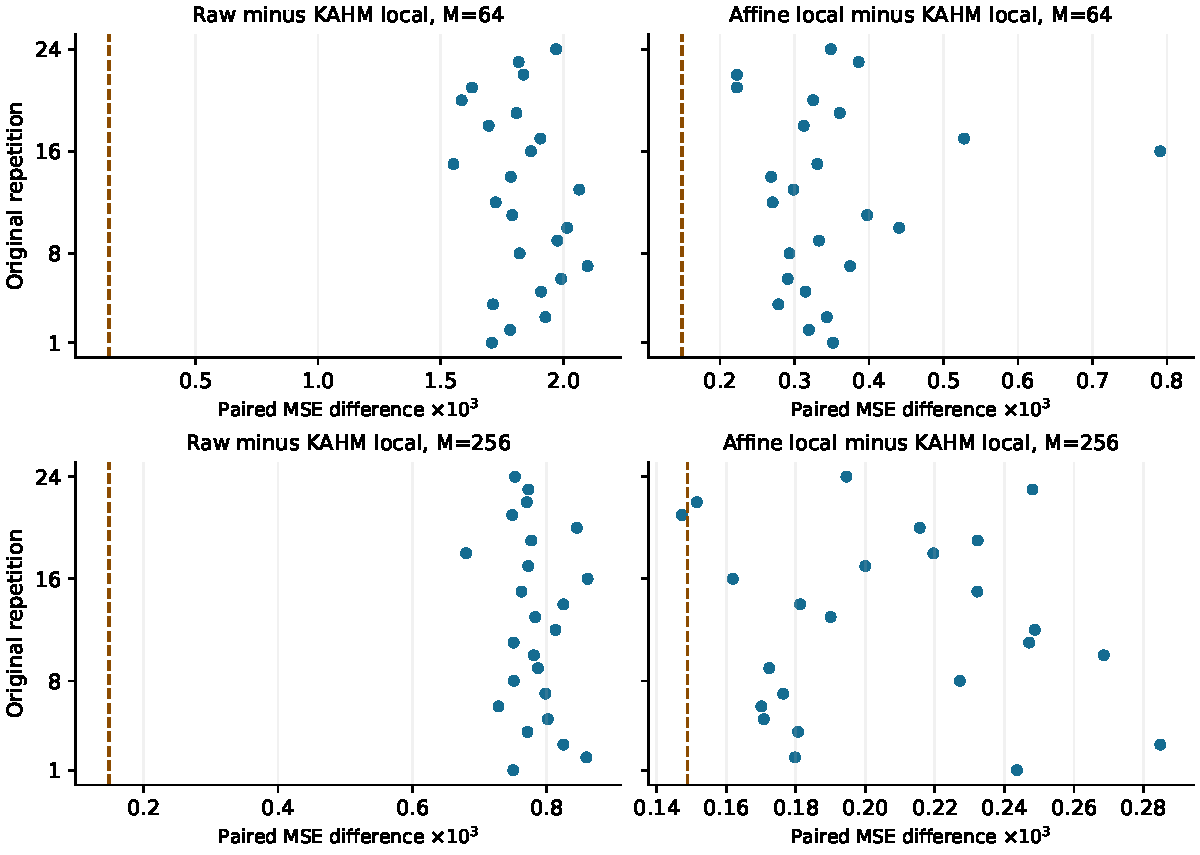
\includegraphics[width=.96\textwidth]{generated/controlled/figures/review_paired_differences.pdf}
\caption{The 24 original paired differences for each Van der Pol capacity comparison,
in units of $10^{-3}$ MSE. The dashed line is the frozen practical margin.
No resampling, refitting, or new primary analysis is performed.}
\label{c:fig:review-paired}
\end{figure}

We also inspect the 120 first-stage primary banks and 72 capacity banks from a
completed computational reproduction using the published seeds. No bank or head is
refitted for these diagnostics. Replayed test inputs, targets, and groups are checked
against their recorded hashes before the original feature map is evaluated.
Let $A$ vertically stack the $P_c^\top$ matrices. Proposition~\ref{c:prop:local-injectivity}
shows that positive gates and full column rank of $A$ suffice to recover the scaled
input from the gated local coordinates and gates:
division by $\phi_c$ recovers $P_c^\top(z-\mu_c)$, after which one solves for $z$.
A deficient stack does not establish information loss in the full code, because the
gates can carry additional information. Numerical ranks use the threshold
$\sigma_1\max\{\text{rows}(A),d\}\epsilon_{64}$; they are finite-precision diagnostics,
not exact rank proofs. Small singular values and small gates can make coordinate
recovery sensitive to perturbations. Test-sample gate minima are not population
lower bounds, and these computations do not guarantee a well-conditioned inverse
or easy decoding by any particular fitted head.
\begin{table}[htbp]
\caption{Retrospective diagnostics over 24 stored banks per row. Rank ranges concern
the stacked local bases in input dimension $d$. The smallest singular value and
gate entries are minima over the inspected banks (and, for gates, their original
test observations); $\kappa_2$ is the largest stack condition number. A dash means
that not every stack in that row has full numerical column rank. KAHM and affine
representations share the basis stack. Computational reproduction supplies no new
independent statistical replications.}
\label{c:tab:review-banks}
\centering\small\setlength{\tabcolsep}{3pt}
% Full column rank is sufficient; numerical ranks are diagnostics, not exact proofs.
\begin{tabular}{llrrrr}
\toprule
Phase / setting & Rank / $d$ & Min. $\sigma_d$ & Max. $\kappa_2$ & Min. $\phi^{\K}$ & Min. $\phi^{\A}$ \\
\midrule
First: Straight branch & 1/2 & $0$ & --- & $3.36\times10^{-25}$ & $2.56\times10^{-20}$ \\
First: Curved branch & 2/2 & $2.19\times10^{0}$ & $1.39\times10^{0}$ & $3.55\times10^{-28}$ & $8.97\times10^{-29}$ \\
First: Nonlinear AR & 12/12 & $6.20\times10^{-2}$ & $4.90\times10^{1}$ & $2.21\times10^{-35}$ & $2.36\times10^{-34}$ \\
First: Van der Pol & 12/12 & $1.60\times10^{-2}$ & $2.20\times10^{2}$ & $2.84\times10^{-45}$ & $9.43\times10^{-20}$ \\
First: Duffing & 12/12 & $1.33\times10^{-2}$ & $2.80\times10^{2}$ & $3.92\times10^{-43}$ & $3.11\times10^{-7}$ \\
Capacity: Nonlinear AR & 12/12 & $7.31\times10^{-2}$ & $4.19\times10^{1}$ & $9.97\times10^{-37}$ & $7.75\times10^{-37}$ \\
Capacity: Van der Pol & 12/12 & $1.60\times10^{-2}$ & $2.19\times10^{2}$ & $6.21\times10^{-44}$ & $1.56\times10^{-16}$ \\
Capacity: Duffing & 12/12 & $1.32\times10^{-2}$ & $2.84\times10^{2}$ & $5.38\times10^{-43}$ & $1.86\times10^{-8}$ \\
\bottomrule
\end{tabular}

\end{table}


\clearpage
\section{Complete controlled results and diagnostics}\label{c:app:tables}

\begin{table}[!htbp]
 \caption{The six primary branch settings at 1,024 training points:
 mean ridge test MSE over 24 repetitions, with the primary KAHM advantage
 $G$ and its interval from the 29-comparison family. The Bayes MSE is
 $1/300$. The affine-locality scoring control reuses the shared references
 and is secondary.}
 \label{c:tab:branch}
 \centering\small\setlength{\tabcolsep}{3pt}
 % Generated by scripts/build_paper_assets.py; do not edit.
\begin{tabular}{rrrrrl}
\toprule
$c$ & $\lambda$ & Affine $\phi$ & KAHM $\phi$ & Affine locality & $G$ [interval] \\
\midrule
0 & 0 & 0.003334 & 0.003347 & 0.003344 & $-0.000013\;[-0.000031,\,0.000005]$ \\
0 & 0.5 & 0.503448 & 0.013995 & 0.003991 & $0.489453\;[0.481962,\,0.496944]$ \\
0 & 1 & 1.002694 & 0.024668 & 0.004641 & $0.978026\;[0.962552,\,0.993500]$ \\
1 & 0 & 0.282887 & 0.281126 & 0.314394 & $0.001761\;[-0.071260,\,0.074781]$ \\
1 & 0.5 & 0.160813 & 0.165207 & 0.167971 & $-0.004395\;[-0.043672,\,0.034882]$ \\
1 & 1 & 0.062366 & 0.051042 & 0.045555 & $0.011324\;[0.000882,\,0.021767]$ \\
\bottomrule
\end{tabular}

\end{table}

\begin{table}[!htbp]
 \caption{All nine first-stage primary settings: mean test MSE over
 24 repetitions for ridge decoders. The local-coordinate improvement $L$
 and its interval belong to the 29-comparison family. Retaining local
 position substantially improves KAHM prediction in eight settings;
 KAHM local coordinates do not dominate affine local coordinates.}
 \label{c:tab:ridge}
 \centering\small\setlength{\tabcolsep}{3pt}
 % Generated by scripts/build_paper_assets.py; do not edit.
\begin{tabular}{lrrrrl}
\toprule
Setting & KAHM $\phi$ & KAHM local & Affine local & Raw & $L$ [interval] \\
\midrule
$c=0,\lambda=0$ & 0.003347 & 0.003378 & 0.003337 & 0.003338 & $-0.000031\;[-0.000043,\,-0.000020]$ \\
$c=0,\lambda=0.5$ & 0.013995 & 0.003379 & 0.003333 & 0.003334 & $0.010616\;[0.010033,\,0.011200]$ \\
$c=0,\lambda=1$ & 0.024668 & 0.003380 & 0.003333 & 0.003330 & $0.021287\;[0.020199,\,0.022376]$ \\
$c=1,\lambda=0$ & 0.281126 & 0.017982 & 0.048916 & 0.671776 & $0.263144\;[0.217187,\,0.309101]$ \\
$c=1,\lambda=0.5$ & 0.165207 & 0.010497 & 0.026756 & 0.337620 & $0.154710\;[0.122867,\,0.186552]$ \\
$c=1,\lambda=1$ & 0.051042 & 0.004188 & 0.004656 & 0.003329 & $0.046854\;[0.040400,\,0.053307]$ \\
Nonlinear AR & 0.005300 & 0.004867 & 0.004867 & 0.005053 & $0.000433\;[0.000368,\,0.000498]$ \\
Van der Pol & 0.111108 & 0.014475 & 0.011582 & 0.041340 & $0.096633\;[0.092436,\,0.100830]$ \\
Duffing & 0.053729 & 0.007560 & 0.004448 & 0.006764 & $0.046168\;[0.041729,\,0.050608]$ \\
\bottomrule
\end{tabular}

\end{table}

\begin{table}[!htbp]
 \caption{Post-hoc Van der Pol numerical sensitivity on the same 24
 second-stage banks and samples. Stable query evaluation removes observed
 zero denominators while leaving local-coordinate mean MSE effectively
 unchanged. $\Delta_r$ is the original-minus-stable MSE difference within
 repetition $r$; wins count stable predictions beating the raw and affine
 local controls at the same width. These comparisons are outside the two primary
 interval families.}
 \label{c:tab:numerical}
 \centering\small
 % Generated by scripts/build_paper_assets.py; do not edit.
\begin{tabular}{lrrrrl}
\toprule
Encoding & $M$ & Original MSE & Stable MSE & Max. $|\Delta_r|$ & Wins raw; affine \\
\midrule
Local & 64 & 0.001026627 & 0.001026627 & $1.01\times10^{-12}$ & 24/24; 24/24 \\
Local & 256 & 0.000871969 & 0.000871969 & $1.69\times10^{-11}$ & 24/24; 24/24 \\
Scores & 64 & 0.001571085 & 0.001565219 & $8.74\times10^{-5}$ & 24/24; 4/24 \\
Scores & 256 & 0.001049909 & 0.001045801 & $3.53\times10^{-5}$ & 24/24; 17/24 \\
\bottomrule
\end{tabular}

\end{table}

\begin{table}[!htbp]
 \caption{Secondary Airfoil static-regression results on one fixed group
 split, averaged over 24 fitting seeds. Units are dB$^2$. These seeds do
 not constitute independent natural-data replications, and the comparison
 is descriptive.}
 \label{c:tab:airfoil}
 \centering\small
 % Generated by scripts/build_paper_assets.py; do not edit.
\begin{tabular}{lrr}
\toprule
Representation & Ridge MSE & RBF$_{64}$ MSE \\
\midrule
Raw & 19.4726 & 15.6898 \\
Affine $\phi$ & 34.1630 & 36.0476 \\
KAHM $\phi$ & 31.8586 & 34.3338 \\
Affine local & 22.7200 & 22.4050 \\
KAHM local & 20.9040 & 20.9313 \\
KAHM scores & 24.2168 & 21.7070 \\
\bottomrule
\end{tabular}

\end{table}

Tables~\ref{c:tab:reconstruction-details} and
\ref{c:tab:reflection-details} give descriptive input-geometry summaries.
The two complete primary comparison families follow. Their values
are generated from the archived outcomes, with each difference,
standard error, interval, and frozen margin independently recomputed
by the paper-asset script before it writes these tables.

\begin{table}[!htbp]
 \caption{Held-out reconstruction errors per standardized input coordinate,
 averaged over the three blocks and 24 full repetitions. ``Best'' takes
 the best local reconstruction separately in each block; ``weighted''
 averages the individual squared errors with that method's affinities.
 The affine value is lower in all 24 repetitions of each of these five
 input settings, for both summaries. These are descriptive diagnostics,
 not the supervised primary endpoint.}
 \label{c:tab:reconstruction-details}
 \centering\small\setlength{\tabcolsep}{4pt}
 % Generated by scripts/build_paper_assets.py; do not edit.
\begin{tabular}{lrrrr}
\toprule
Setting & KAHM best & Affine best & KAHM weighted & Affine weighted \\
\midrule
Branch $c=0$ & $3.276\times10^{-3}$ & $2.156\times10^{-16}$ & $4.006\times10^{-3}$ & $1.548\times10^{-8}$ \\
Branch $c=1$ & $3.583\times10^{-2}$ & $2.932\times10^{-2}$ & $3.793\times10^{-2}$ & $3.238\times10^{-2}$ \\
Nonlinear AR & $1.166\times10^{-2}$ & $1.084\times10^{-2}$ & $1.305\times10^{-2}$ & $1.214\times10^{-2}$ \\
Van der Pol & $4.353\times10^{-3}$ & $1.683\times10^{-3}$ & $4.495\times10^{-3}$ & $1.916\times10^{-3}$ \\
Duffing & $4.877\times10^{-3}$ & $5.613\times10^{-4}$ & $5.239\times10^{-3}$ & $1.226\times10^{-3}$ \\
\bottomrule
\end{tabular}

\end{table}

\begin{table}[!htbp]
 \caption{Branch reflection differences at training size 1,024, averaged
 over 24 banks. The statistic is a per-coordinate RMS, with and without
 training-only coordinate scaling. The raw reflection precedes the
 frozen pipeline. These values neither establish exact information
 loss for the learned code nor certify a decoder-specific population
 risk bound.}
 \label{c:tab:reflection-details}
 \centering\small\setlength{\tabcolsep}{5pt}
 % Generated by scripts/build_paper_assets.py; do not edit.
\begin{tabular}{rlrr}
\toprule
$c$ & Encoding & Stored-coordinate RMS & Standardized RMS \\
\midrule
0 & KAHM $\phi$ & $4.894\times10^{-1}$ & $1.402\times10^{0}$ \\
0 & Affine $\phi$ & $1.451\times10^{-9}$ & $7.533\times10^{-9}$ \\
0 & KAHM local & $5.289\times10^{-1}$ & $1.418\times10^{0}$ \\
0 & Affine local & $4.993\times10^{-1}$ & $1.236\times10^{0}$ \\
1 & KAHM $\phi$ & $5.380\times10^{-1}$ & $1.427\times10^{0}$ \\
1 & Affine $\phi$ & $5.321\times10^{-1}$ & $1.471\times10^{0}$ \\
1 & KAHM local & $4.854\times10^{-1}$ & $1.442\times10^{0}$ \\
1 & Affine local & $5.522\times10^{-1}$ & $1.473\times10^{0}$ \\
\bottomrule
\end{tabular}

\end{table}

\begin{table}[!htbp]
 \caption{Complete representation means in the fresh capacity study,
 with MSE multiplied by $10^3$. The full-score KAHM representation is
 a prespecified secondary control. These point estimates do not add
 hypotheses to the 12-comparison primary family.}
 \label{c:tab:capacity-means-details}
 \centering\small\setlength{\tabcolsep}{4pt}
 % Generated by scripts/build_paper_assets.py; do not edit.
\begin{tabular}{lrrrrr}
\toprule
System & $M$ & Raw & Affine local & KAHM local & KAHM scores \\
\midrule
Nonlinear AR & 64 & 4.4238 & 4.9120 & 4.8795 & 4.7984 \\
Nonlinear AR & 256 & 4.6958 & 5.2347 & 5.1749 & 4.8256 \\
Van der Pol & 64 & 2.8586 & 1.3767 & 1.0266 & 1.5711 \\
Van der Pol & 256 & 1.6541 & 1.0780 & 0.8720 & 1.0499 \\
Duffing & 64 & 3.4597 & 3.0549 & 4.2154 & 4.7005 \\
Duffing & 256 & 2.8364 & 2.7981 & 4.0736 & 3.3808 \\
\bottomrule
\end{tabular}

\end{table}

\clearpage
\subsection{Selected pipelines and realized dimensions}

The validation-selected pipeline and the retained nonlinear basis are
distinct summaries: the former describes the operational model choice,
whereas the latter records the realized dimensions behind the nominal
landmark budgets.

\begin{table}[!htbp]
 \caption{Secondary validation-only selection among the eight complete
 capacity-study pipelines. Mean test MSE is multiplied by $10^3$.
 Counts concern independent complete repetitions under each generator,
 not a new population of forecasting tasks.}
 \label{c:tab:capacity-selector-details}
 \centering\small\setlength{\tabcolsep}{4pt}
 % Generated by scripts/build_paper_assets.py; do not edit.
\begin{tabular}{lrl}
\toprule
System & Selector MSE & Validation selections \\
\midrule
Nonlinear AR & 4.4238 & Raw, 64: 24/24 \\
Van der Pol & 0.8720 & KAHM local, 256: 24/24 \\
Duffing & 2.7923 & Affine local, 256: 23/24; Raw, 256: 1/24 \\
\bottomrule
\end{tabular}

\end{table}

\begin{table}[!htbp]
 \caption{Retained RBF-plus-linear dimensions after the Nystr\"om
 eigenvalue cutoff in the fresh capacity study. Means and ranges cover
 the 24 repetitions in each cell. The same landmark count $M$ does not
 imply the same realized dimension or function class.}
 \label{c:tab:capacity-dimensions-details}
 \centering\small\setlength{\tabcolsep}{5pt}
 % Generated by scripts/build_paper_assets.py; do not edit.
\begin{tabular}{lrlrr}
\toprule
System & $M$ & Representation & Mean dimension & Range \\
\midrule
Nonlinear AR & 64 & Raw & 74.88 & 61--76 \\
Nonlinear AR & 64 & Affine local & 106.00 & 106--106 \\
Nonlinear AR & 64 & KAHM local & 106.00 & 106--106 \\
Nonlinear AR & 64 & KAHM scores & 76.71 & 62--78 \\
Nonlinear AR & 256 & Raw & 189.04 & 78--268 \\
Nonlinear AR & 256 & Affine local & 297.62 & 296--298 \\
Nonlinear AR & 256 & KAHM local & 297.50 & 293--298 \\
Nonlinear AR & 256 & KAHM scores & 148.88 & 77--219 \\
Van der Pol & 64 & Raw & 76.00 & 76--76 \\
Van der Pol & 64 & Affine local & 106.00 & 106--106 \\
Van der Pol & 64 & KAHM local & 106.00 & 106--106 \\
Van der Pol & 64 & KAHM scores & 78.00 & 78--78 \\
Van der Pol & 256 & Raw & 268.00 & 268--268 \\
Van der Pol & 256 & Affine local & 298.00 & 298--298 \\
Van der Pol & 256 & KAHM local & 272.38 & 261--285 \\
Van der Pol & 256 & KAHM scores & 231.88 & 215--251 \\
Duffing & 64 & Raw & 76.00 & 76--76 \\
Duffing & 64 & Affine local & 106.00 & 106--106 \\
Duffing & 64 & KAHM local & 105.46 & 98--106 \\
Duffing & 64 & KAHM scores & 77.96 & 77--78 \\
Duffing & 256 & Raw & 268.00 & 268--268 \\
Duffing & 256 & Affine local & 296.92 & 272--298 \\
Duffing & 256 & KAHM local & 240.38 & 176--298 \\
Duffing & 256 & KAHM scores & 214.33 & 164--270 \\
\bottomrule
\end{tabular}

\end{table}

\clearpage
% Generated; this file owns its longtable environment.
\begingroup\small\setlength{\tabcolsep}{3pt}
\begin{longtable}{llrrrl}
\caption{Complete first-stage family (29 contrasts), in original MSE units. Intervals use the two-sided 95\% Bonferroni paired-replicate Student procedure with 23 degrees of freedom. Under paired normality, each t interval is exact and Bonferroni family coverage is at least 95\%; otherwise coverage is approximate. The two stages have separate families.}\label{c:tab:all-stageone}\\
\toprule
Setting / budget & Contrast & $\overline D$ & Simultaneous interval & $\delta$ & Assessment \\
\midrule
\endfirsthead
\toprule
Setting / budget & Contrast & $\overline D$ & Simultaneous interval & $\delta$ & Assessment \\
\midrule
\endhead
\bottomrule\endfoot
$c=0,\lambda=0$ & $G$ & -0.000013 & $[-0.000031,\,0.000005]$ & 0.000168 & unresolved $\dagger$ \\
$c=0,\lambda=0$ & $N$ & -0.000008 & $[-0.000016,\,\ensuremath{-1.85\times10^{-7}}]$ & 0.000168 & negative $\dagger$ \\
$c=0,\lambda=0$ & $L$ & -0.000031 & $[-0.000043,\,-0.000020]$ & 0.000168 & negative $\dagger$ \\
$c=0,\lambda=0.5$ & $G$ & 0.489453 & $[0.481962,\,0.496944]$ & 0.000168 & practical + \\
$c=0,\lambda=0.5$ & $N$ & 0.000944 & $[0.000088,\,0.001799]$ & 0.000168 & positive \\
$c=0,\lambda=0.5$ & $L$ & 0.010616 & $[0.010033,\,0.011200]$ & 0.000168 & practical + \\
$c=0,\lambda=1$ & $G$ & 0.978026 & $[0.962552,\,0.993500]$ & 0.000168 & practical + \\
$c=0,\lambda=1$ & $N$ & 0.001938 & $[0.000255,\,0.003621]$ & 0.000168 & practical + \\
$c=0,\lambda=1$ & $L$ & 0.021287 & $[0.020199,\,0.022376]$ & 0.000168 & practical + \\
$c=1,\lambda=0$ & $G$ & 0.001761 & $[-0.071260,\,0.074781]$ & 0.033542 & unresolved \\
$c=1,\lambda=0$ & $N$ & 0.069128 & $[0.028663,\,0.109593]$ & 0.033542 & positive \\
$c=1,\lambda=0$ & $L$ & 0.263144 & $[0.217187,\,0.309101]$ & 0.033542 & practical + \\
$c=1,\lambda=0.5$ & $G$ & -0.004395 & $[-0.043672,\,0.034882]$ & 0.016863 & unresolved \\
$c=1,\lambda=0.5$ & $N$ & 0.040663 & $[0.019789,\,0.061538]$ & 0.016863 & practical + \\
$c=1,\lambda=0.5$ & $L$ & 0.154710 & $[0.122867,\,0.186552]$ & 0.016863 & practical + \\
$c=1,\lambda=1$ & $G$ & 0.011324 & $[0.000882,\,0.021767]$ & 0.000168 & practical + \\
$c=1,\lambda=1$ & $N$ & 0.012111 & $[0.005647,\,0.018574]$ & 0.000168 & practical + \\
$c=1,\lambda=1$ & $L$ & 0.046854 & $[0.040400,\,0.053307]$ & 0.000168 & practical + \\
Nonlinear AR & $G$ & \ensuremath{-1.89\times10^{-7}} & $[-0.000050,\,0.000049]$ & 0.000253 & unresolved $\dagger$ \\
Nonlinear AR & $N$ & -0.000016 & $[-0.000062,\,0.000029]$ & 0.000253 & unresolved $\dagger$ \\
Nonlinear AR & $L$ & 0.000433 & $[0.000368,\,0.000498]$ & 0.000253 & practical + \\
Van der Pol & $G$ & -0.049419 & $[-0.060532,\,-0.038307]$ & 0.002036 & negative \\
Van der Pol & $N$ & 0.013443 & $[0.005084,\,0.021803]$ & 0.002036 & practical + \\
Van der Pol & $L$ & 0.096633 & $[0.092436,\,0.100830]$ & 0.002036 & practical + \\
Duffing & $G$ & -0.030948 & $[-0.035414,\,-0.026482]$ & 0.000338 & negative \\
Duffing & $N$ & 0.005558 & $[0.001721,\,0.009395]$ & 0.000338 & practical + \\
Duffing & $L$ & 0.046168 & $[0.041729,\,0.050608]$ & 0.000338 & practical + \\
$c=0$ interaction & $I_0$ & -0.978039 & $[-0.993512,\,-0.962566]$ & 0.000168 & opposite sign \\
$c=1$ interaction & $I_1$ & -0.009564 & $[-0.082839,\,0.063712]$ & 0.016855 & unresolved \\
\end{longtable}
\noindent $\dagger$: the entire interval lies within the fixed practical band $[-\delta,\delta]$. An unresolved sign alone does not establish equivalence.
\endgroup

\clearpage
% Generated; this file owns its longtable environment.
\begingroup\small\setlength{\tabcolsep}{3pt}
\begin{longtable}{llrrrl}
\caption{Complete fresh capacity family (12 contrasts). All numerical loss quantities are multiplied by $10^3$. Intervals use the two-sided 95\% Bonferroni paired-replicate Student procedure with 23 degrees of freedom. Under paired normality, each t interval is exact and Bonferroni family coverage is at least 95\%; otherwise coverage is approximate. The two stages have separate families.}\label{c:tab:all-capacity}\\
\toprule
Setting / budget & Contrast & $\overline D$ & Simultaneous interval & $\delta$ & Assessment \\
\midrule
\endfirsthead
\toprule
Setting / budget & Contrast & $\overline D$ & Simultaneous interval & $\delta$ & Assessment \\
\midrule
\endhead
\bottomrule\endfoot
Nonlinear AR / 64 & Raw--K & -0.4556 & $[-0.5235,\,-0.3878]$ & 0.2201 & negative \\
Nonlinear AR / 64 & Affine--K & 0.0325 & $[-0.0031,\,0.0680]$ & 0.2201 & unresolved $\dagger$ \\
Nonlinear AR / 256 & Raw--K & -0.4791 & $[-0.6013,\,-0.3569]$ & 0.2201 & negative \\
Nonlinear AR / 256 & Affine--K & 0.0598 & $[-0.0131,\,0.1327]$ & 0.2201 & unresolved $\dagger$ \\
Van der Pol / 64 & Raw--K & 1.8320 & $[1.7369,\,1.9271]$ & 0.1489 & practical + \\
Van der Pol / 64 & Affine--K & 0.3501 & $[0.2755,\,0.4247]$ & 0.1489 & practical + \\
Van der Pol / 256 & Raw--K & 0.7822 & $[0.7550,\,0.8094]$ & 0.1489 & practical + \\
Van der Pol / 256 & Affine--K & 0.2060 & $[0.1810,\,0.2311]$ & 0.1489 & practical + \\
Duffing / 64 & Raw--K & -0.7557 & $[-1.0831,\,-0.4282]$ & 0.1727 & negative \\
Duffing / 64 & Affine--K & -1.1605 & $[-1.4707,\,-0.8503]$ & 0.1727 & negative \\
Duffing / 256 & Raw--K & -1.2372 & $[-1.5242,\,-0.9503]$ & 0.1727 & negative \\
Duffing / 256 & Affine--K & -1.2756 & $[-1.5702,\,-0.9810]$ & 0.1727 & negative \\
\end{longtable}
\noindent $\dagger$: the entire interval lies within the fixed practical band $[-\delta,\delta]$. An unresolved sign alone does not establish equivalence.
\endgroup


\section{Representations and fitted forecasting rules}
\label{sec:nf-methods}

A history $x\in\mathbb R^d$ contains the observations available at a forecast
origin; its response $y\in\mathbb R^H$ contains the next $H$ observations.
For the univariate tasks below, the input dimension $d$ equals the history length $L$.
We fit direct multioutput regressors to historical pairs
$\{(x_i,y_i)\}_{i=1}^n$.  The construction below specifies which part of the
regressor uses KAHM geometry.  It does not assume that overlapping forecasting
windows are independent.  All input transformations, reference sets, and
decoder bases are fitted on the training portion of each fit.

\subsection{Shared reference geometry}
\label{sec:nf-reference-geometry}

Write $z(x)=D^{-1}(x-\bar x)$, where $\bar x$ and the diagonal scales $D$ are
training means and population standard deviations.  A standard deviation at
most $10^{-12}$ is replaced by one.  Thus this transformation retains every
raw coordinate, including coordinates constant in the observed training set.
Three independently seeded $k$-means partitions, with $k\in\{2,4,8\}$, use
the same seeded subset of at most 512 training histories.  Each partition has
five initializations and at most 150 iterations.  Each cluster supplies at
most 24 references sampled without replacement; all its rows are used if
there are fewer.  For a common seed and training set, the alternative gates
use identical partition and reference-selection rules.  They are nevertheless
fitted as separate computational pipelines.

Index the 14 local models by $c$, with the partition blocks denoted
$\mathcal C_b$.  Let
$Q_c=[q_{c1},\ldots,q_{cm_c}]\in\mathbb R^{d\times m_c}$ contain the
training-standardized references, stored after the inherited float32
conversion, and let $\mu_c=m_c^{-1}Q_c\mathbf 1$.
The orthonormal columns of $P_c\in\mathbb R^{d\times r_c}$ are leading
eigenvectors of the centered reference covariance.  The requested rank is
$\min(2,d-1,m_c-1)$; only eigenvalues above double-precision machine epsilon
are retained.  The inherited implementation further reduces a rank greater
than one if the smallest projected coordinate range is below $10^{-3}$.
A reference set with no usable direction has $r_c=0$ and uses its center as
its reconstruction.  Other numerical failures remain recorded failures.

The affine reconstruction and centered local coordinates are
\begin{equation}
 a_c(z)=\mu_c+P_cP_c^\top(z-\mu_c),
 \qquad u_c(z)=P_c^\top(z-\mu_c).
 \label{eq:nf-affine}
\end{equation}
The affine and locality controls compute these quantities without fitting or
querying any KAHM kernel.

\subsection{Reconstruction scores and local gates}
\label{sec:nf-gates}

\paragraph{KAHM reconstruction.}
Kernel Affine Hull Machines construct nonlinear reconstructions from local
kernel weights \citep{Kumar2024KAHM}.  We retain the pinned implementation's
local autoencoder, rather than asserting equivalence to an independently
optimized end-to-end KAHM learner.  For $r_c>0$, let $\Sigma_c$ be the sample
covariance of the columns of $P_c^\top Q_c$.  Its Gaussian kernel is
\begin{equation}
 k_c(z,q)=\exp\!\left\{-\frac{
  (P_c^\top(z-q))^\top\Sigma_c^{-1}P_c^\top(z-q)}{2r_c}\right\},
 \qquad (K_c)_{ij}=k_c(q_{ci},q_{cj}).
 \label{eq:nf-kahm-kernel}
\end{equation}
To specify the inherited local regularizer exactly, put
$\nu_c=\|Q_c\|_F^2/(dm_c)$ and initialize $\lambda_0=5\nu_c/2$.  Its iteration is
\begin{equation}
 B_t=(K_c+\lambda_t I)^{-1},\qquad
 \lambda_{t+1}=2\nu_c+
 \frac{\|Q_c-Q_c(K_cB_t)^\top\|_F^2}{dm_c}.
 \label{eq:nf-local-regularizer}
\end{equation}
It stops after an update of size at most $10^{-3}$ or 100 updates, and
retains the last computed $B_t$ as $B_c$.  In particular, it does not perform
an extra inverse at the newly updated $\lambda_{t+1}$.
For $k_c(z)=(k_c(z,q_{cj}))_{j=1}^{m_c}$, define
\begin{equation}
 v_c(z)=B_c^\top k_c(z),\qquad
 \widehat z_c(z)=\frac{Q_cv_c(z)}{\mathbf 1^\top v_c(z)}.
 \label{eq:nf-reconstruction}
\end{equation}
The weights may be signed.  The reconstruction is therefore not generally a
convex average.  The inherited exact-zero-denominator convention replaces
the denominator by one; that convention is an implementation choice, not
a definition of a continuous extension at a singularity.

\paragraph{Stable Gaussian evaluation.}
For queries we compute the analytic log kernel
$\ell_{cj}(z)=-\|S_cP_c^\top(z-q_{cj})\|^2/(2r_c)$, where $S_c$ is the
stored symmetric square root of the inverse covariance, and use
$\widetilde k_{cj}(z)=\exp\{\ell_{cj}(z)-\max_j\ell_{cj}(z)\}$ in
Equation~\eqref{eq:nf-reconstruction}.
In exact arithmetic, $S_c^\top S_c=\Sigma_c^{-1}$, and multiplying every
kernel entry for one query by the same positive constant cancels from the
normalized reconstruction whenever its denominator is nonzero.
This calculation avoids underflow caused solely by a large common negative
log-kernel offset.  It does not prevent signed cancellation, guarantee a
well-conditioned denominator, or guarantee equivalence at an exact zero.
The implementation retains the zero-denominator convention, records numerical
diagnostics, and rejects nonfinite outputs.  The historical mode instead
exponentiates the unshifted logs through the inherited query routine; it is
retained for equivalence checks, while this study uses the shifted evaluation.

\paragraph{Matched folding gates.}
Given either the KAHM reconstruction $\widehat z_c$ or the affine
reconstruction $a_c$, denote it by $r_c^{\mathrm{rec}}(z)$.  Define
\begin{align}
 \rho_c(z)&=1-\exp\{-\|z-r_c^{\mathrm{rec}}(z)\|\},\qquad
 \theta_c(z)=\frac1\pi\arccos\!\left(
 \operatorname{clip}_{[-1,1]}
 \frac{z^\top r_c^{\mathrm{rec}}(z)}{\|z\|\,\|r_c^{\mathrm{rec}}(z)\|}\right),
 \notag\\
 s_c(z)&=\sqrt{\{\rho_c(z)^2+\theta_c(z)^2\}/2},\qquad
 \phi_c(z)=\frac{[1-\operatorname{clip}_{[0,1]}s_c(z)+\tau]^\omega}
 {\sum_{j\in\mathcal C_b}[1-\operatorname{clip}_{[0,1]}s_j(z)+\tau]^\omega},
 \quad c\in\mathcal C_b.
 \label{eq:nf-folding-gates}
\end{align}
When either norm in the cosine denominator is zero, its cosine is set to
zero, so that $\theta_c=1/2$.  The fixed values are $\omega=16$ and
$\tau=10^{-6}$; normalization is evaluated with log-sum-exp.  The comparison
between these two gates changes the reconstruction while retaining the
score, reference geometry, and local-coordinate construction.

\paragraph{Locality control.}
The third gate uses the historical native-affine score formula, applied to
the same references.  With $\epsilon=10^{-6}$, set
\begin{align}
 t_c&=\max\!\left\{m_c^{-1}\sum_j\|q_{cj}-\mu_c\|^2,\epsilon\right\},\notag\\
 e_c&=\max\!\left\{m_c^{-1}\sum_j\|q_{cj}-a_c(q_{cj})\|^2,
                    0.05t_c,\epsilon\right\},\notag\\
 b_c(z)&=\frac{\|z-a_c(z)\|^2}{e_c}
          +0.1\frac{\|z-\mu_c\|^2}{t_c},\notag\\
 \phi_c(z)&=\frac{\exp[-b_c(z)]}
                    {\sum_{j\in\mathcal C_b}\exp[-b_j(z)]}.
 \label{eq:nf-locality-gates}
\end{align}
This distinguishes proximity to the local center from projection residual.
Here ``native'' identifies a score formula; it does not identify a separately
tuned native learning algorithm.  It supplies a non-KAHM locality alternative
to the matched folding-score comparison.

\subsection{Local codes and finite forecasting heads}
\label{sec:nf-local-features}

For each gate family $g$, concatenate all gates and gated local coordinates:
\begin{equation}
 T_g(x)=\bigl((\phi_c(z(x)))_c,
                  (\phi_c(z(x))u_c(z(x)))_c\bigr),\qquad
 T_{\mathrm{raw}+g}(x)=(z(x),T_g(x)).
 \label{eq:nf-local-code}
\end{equation}
The stored local width is $14+\sum_c r_c\leq42$; the actual width is recorded.
The raw augmentation prepends all $d$ history coordinates, with no truncation
when $d>28$.  The combination of local association and local position is
related to coordinate and tangent coding \citep{Yu2009LCC,Yu2010LTC};
our gates and decoder are the explicit constructions above.
The stack of $P_c^\top$ has rank at most 28.  A deficient stack alone does
not prove information loss in $T_g$, because the gates also depend on the
query.  Raw augmentation gives the simpler unconditional reconstruction
property stated below, without a rank assumption.

\paragraph{Nystr\"om plus linear basis.}
\label{sec:nf-head}
Let $v(x)$ denote $z(x)$, $T_g(x)$, or $T_{\mathrm{raw}+g}(x)$, and let
$q(x)$ be its coordinatewise training standardization.  Select $M$ training
rows without replacement as landmarks $a_1,\ldots,a_M$ in $q$-space.
The requested $M$ is 32 or 64, capped by the training size.
Set $\sigma^2$ to the median positive squared inter-landmark distance and
define
\begin{equation}
 k_\sigma(q,a)=\exp\{-\|q-a\|^2/(2\sigma^2)\},\qquad
 b(x)=\left(q(x),\;
       \operatorname{diag}(\eta_J^{-1/2})U_J^\top
                  (k_\sigma(q(x),a_j))_{j=1}^M\right).
 \label{eq:nf-nystrom}
\end{equation}
Here $U\operatorname{diag}(\eta)U^\top$ diagonalizes the landmark Gram
matrix, and $J$ retains eigenvalues exceeding
$\max(10^{-10}\eta_{\max},10^{-12})$ \citep{Williams2001Nystrom}.
Distances at most $10^{-14}$ are excluded from the bandwidth median;
if none remain the squared bandwidth is one, and in all cases it is floored
at $10^{-12}$.  The bandwidth multiplier is fixed to one.
Finally, standardize $b$ on training rows to obtain $f(x)$ and the design
$F_{i,:}=f(x_i)^\top$.  Both head standardizations replace scales below
$10^{-8}$ by one.  Raw ridge omits the Nystr\"om block and uses the same
centering and scaling convention.

For each horizon $h$, the fitted decoder solves
\begin{equation}
 \min_{\beta_h,a_h}\ \frac1n\sum_{i=1}^n
       [y_{ih}-a_h-f(x_i)^\top\beta_h]^2+\alpha\|\beta_h\|^2.
 \label{eq:nf-ridge-objective}
\end{equation}
Thus the normal equations use $F^\top F/n+\alpha I$, and the intercept is
unpenalized.  Internally, targets are standardized using training statistics
and transformed back after prediction.  For fixed $\alpha$, linearity makes
this exactly equivalent in real arithmetic to
Equation~\eqref{eq:nf-ridge-objective} in the original target units.
This is a Euclidean ridge penalty on a standardized finite basis, rather
than the canonical Gaussian RKHS norm.  Adding local features also changes
the Gaussian distances and the resulting Nystr\"om basis; the raw and
augmented nonlinear decoder classes need not be nested.

One common $\alpha$ from the ordered grid $(0.01,1,100)$ is selected by validation MSE averaged
over origins and horizons in original target units, with the first grid
entry winning ties.  Within a method, geometry, training and validation
features, basis construction, and the Gram eigensystem are computed once;
all three alphas reuse those quantities.  Different method variants share
no fitted bank or free preprocessing.  The selected configuration is then
fitted anew on the admissible pretest training data.  Search designs and
eigensystems are not retained in the serialized final model.  This gives
an explicit efficient search whose full computation can be measured.

\subsection{Information and finite-decoder risk}
\label{sec:nf-information}

The following elementary facts delimit the interpretation of the experiments.
They are established information-preservation and linear-smoother algebra,
not new KAHM approximation theorems or performance guarantees.

\begin{proposition}[Information preserved by raw augmentation]
\label{prop:nf-raw-preservation}
Condition on a fitted state $\Theta$ containing $\bar x$, positive diagonal
$D$, and a measurable, finite-valued feature map $T_g$ on the support of $X$.
Then $T_{\mathrm{raw}+g}(X)$ and $X$ generate the same information conditional
on $\Theta$.  For a square-integrable response $Y$, their conditional
expectations and optimal squared-loss Bayes risks coincide, conditional on
$\Theta$.  This statement requires neither positive gates nor a full-rank
stack of local bases.
\end{proposition}
\begin{proof}
The augmented code is a measurable function of $(X,\Theta)$, and its first
$d$ coordinates recover $X=\bar x+Dz(X)$.  Consequently
$\sigma(T_{\mathrm{raw}+g}(X),\Theta)=\sigma(X,\Theta)$.
Conditional expectation onto these equal sigma-fields, and hence the
minimum squared prediction error, is identical.
\end{proof}

This is an exact-arithmetic statement about the representation, not a
conditioning guarantee or a claim that a particular fitted decoder uses
every retained coordinate.  Empirical gains from raw augmentation must
therefore be explained through finite fitting, representation-dependent
regularization, or numerical behavior, rather than increased Bayes
information relative to the same raw input.

\begin{proposition}[Fixed-feature, fixed-alpha risk identity]
\label{prop:nf-linear-risk}
Consider one response coordinate, a fixed $\alpha>0$, and the centered
training design $F$ above.  Let $\mathcal G$ contain the training and query
inputs and the randomness used to fit their unsupervised feature map, so
$F$ and $f(x_*)$ are $\mathcal G$-measurable.  Put
\begin{equation}
 w_* = \frac{\mathbf 1}{n}
       +F(F^\top F+n\alpha I)^{-1}f(x_*).
 \label{eq:nf-smoother}
\end{equation}
Let the training response vector be $Y$, the future response be $Y_*$, and
assume their conditional second moments are finite.  Define
$\mu=\mathbb E[Y\mid\mathcal G]$,
$\mu_*=\mathbb E[Y_*\mid\mathcal G]$,
$\Sigma=\operatorname{Cov}(Y\mid\mathcal G)$,
$c=\operatorname{Cov}(Y,Y_*\mid\mathcal G)$, and
$v_*=\operatorname{Var}(Y_*\mid\mathcal G)$.  The fitted prediction is
$\widehat Y_*=w_*^\top Y$, and
\begin{equation}
 \mathbb E[(\widehat Y_*-Y_*)^2\mid\mathcal G]
   =(w_*^\top\mu-\mu_*)^2+w_*^\top\Sigma w_*+v_*-2w_*^\top c.
 \label{eq:nf-dependent-risk}
\end{equation}
\end{proposition}
\begin{proof}
Because $F^\top\mathbf 1=0$, the unpenalized intercept is $\bar Y$ and
$\widehat\beta=(F^\top F+n\alpha I)^{-1}F^\top Y$.
Substituting into $\bar Y+f(x_*)^\top\widehat\beta$ gives
Equation~\eqref{eq:nf-smoother}; the inverse target standardization cancels
as described above.  Conditional on $\mathcal G$, expand the second moment
of $w_*^\top Y-Y_*$ as its squared mean plus its variance.  The covariance
cross term is $-2w_*^\top c$, giving the identity.
\end{proof}

The identity holds without independent training responses or an independent
future response.  Overlapping windows and serial dependence can affect both
$\Sigma$ and $c$; neither may be discarded without additional assumptions.
Averaging the identity over horizons gives the corresponding average risk.
Changing geometry changes $w_*$ and can change all its bias and covariance
terms, without a universal ordering between representations.  The identity
does not automatically describe the full validation-selected procedure:
after alpha selection, the smoother depends on observed validation responses.
No generalization or selection guarantee is inferred from it.

\section{Natural-data protocol}
\label{sec:nf-protocol}

Source allocation, task roster, model grids, and analysis are fixed before
comparative outcomes.  The evaluation compares matched representations, accuracy and computational
cost, and prospective model selection on reserved source families. The
reproduction materials include specifications, input checksums, and source
checkpoints. The study was not externally preregistered.

\subsection{Sources and chronological tasks}
\label{sec:nf-data}

Table~\ref{tab:nf-sources} gives eight versioned Monash snapshots
\citep{Godahewa2021Monash}, chosen by provenance, application diversity, length,
and size.  Related series, channels, and aggregations share a source family
and cannot cross the boundary between development and confirmation.  Models are local to
each series, including differently dated Tourism series.  The supplement
retains the records' CC BY 4.0 licenses, versions, attribution, original-source
references, and archive hashes.

\begin{table}[t]
\caption{Fixed source allocation and forecast regimes.  ``Selected/all'' counts
series, not independent source families.  Each selected series uses both regimes
for its frequency.  $L$ is history length, $H$ forecast horizon, and $s$ the
declared seasonal period.}
\label{tab:nf-sources}
\centering\small
\setlength{\tabcolsep}{4pt}
\begin{tabular}{@{}lp{0.48\linewidth}cr@{}}
\toprule
Phase & Source snapshot & Frequency & Selected/all \\
\midrule
Development & Electricity \citep{DatasetElectricityWeekly} & weekly & 4/321 \\
 & NN5, with missing values \citep{DatasetNN5Daily} & daily & 4/111 \\
 & Tourism \citep{DatasetTourismMonthly} & monthly & 4/366 \\
 & FRED-MD \citep{DatasetFREDMD} & monthly & 4/107 \\
\midrule
Confirmation & Traffic \citep{DatasetTrafficWeekly} & weekly & 4/862 \\
 & Hospital \citep{DatasetHospitalMonthly} & monthly & 4/767 \\
 & Saugeen River flow \citep{DatasetSaugeenDaily} & daily & 1/1 \\
 & US births \citep{DatasetUSBirthsDaily} & daily & 1/1 \\
\bottomrule
\end{tabular}
\par\medskip
\begin{tabular}{@{}lccc@{}}
\toprule
Frequency & Short $(L,H)$ & Long $(L,H)$ & $s$ \\
\midrule
Monthly & $(12,3)$ & $(24,6)$ & 12 \\
Weekly & $(13,4)$ & $(26,8)$ & 52 \\
Daily & $(28,7)$ & $(56,14)$ & 7 \\
\bottomrule
\end{tabular}
\end{table}

Training-prefix eligibility requires at least 16 finite windows in each regime
and a positive training error scale.  A fixed salted hash of source and series
ID orders eligible series; we retain the first four, or all if fewer exist,
across regimes and capacities.  No later loss or availability criterion selects
replacements.  The 26 series give 52 base tasks; two capacities and seeds 17
and 43 give 208 runs: 128 development and 80 confirmation, with four source
families per phase.

For a length-$n$ series indexed from zero, let
$a=\lfloor3n/5\rfloor$ and $b=\lfloor4n/5\rfloor$.  Training, validation, and
test intervals are $[0,a)$, $[a,b)$, and $[b,n)$.  An origin $t$ is the last
observed index, with
\begin{equation}
 x_t=(y_{t-L+1},\ldots,y_t)^\top,\qquad
 y_t^+=(y_{t+1},\ldots,y_{t+H})^\top.
 \label{eq:nf-forecast-window}
\end{equation}
The complete target interval must lie within its split; contexts may include
earlier observed values.  Stateful controls receive $t+1$, their first-future
index.  We retain raw snapshot values, including NN5 missing markers, and
discard windows with an unavailable context or target without interpolation.
Evenly spaced indices among available origins give at most 64 validation and
64 test windows, and the training cap in Table~\ref{tab:nf-capacity}.  Every
method receives the same evaluation origins.

Before outcomes, length checks reduced the proposed monthly $(48,6)$ and
weekly $(52,8)$ regimes, which yield zero Hospital and three Traffic training
windows.  The adopted long regimes yield 21 and 29, respectively.  Context
and horizon are paired, so their separate effects are not identified.
NN5 T88 at $(56,14)$ retains only seven test origins out of 146 candidates.
All task availability counts are recorded.

All candidate preprocessing is fitted on training data, and validation MSE
selects hyperparameters.  The selected pipeline is then fitted anew on all
eligible windows with targets preceding $b$, subject to its training cap.
This refit includes windows crossing the former training/validation
boundary because all their targets precede the test segment.  Parameters are fixed thereafter; earlier realized observations may
enter later contexts or state updates.  Test outcomes never retune parameters.

\subsection{Comparators, capacity, and loss}
\label{sec:nf-comparators}

The twelve methods comprise raw ridge and raw RBF heads; affine-, locality-,
and KAHM-gated local RBF pipelines; each local pipeline augmented by the full
raw history; and seasonal naive, Holt, histogram gradient boosting, and a
one-hidden-layer MLP.  Section~\ref{sec:nf-methods} defines the feature maps and
finite RBF head.  The primary matched pair is raw RBF ($R$) versus raw-history
plus KAHM RBF ($K$).  The raw-history controls retain the inputs independently
of local-basis rank (Proposition~\ref{prop:nf-raw-preservation}).  The evaluation reports every method in this twelve-method portfolio.

The geometric bank uses cluster counts $(2,4,8)$, requested rank two, at most
24 references per local model, a 512-row fitting cap, $\omega=16$, and
$\tau=10^{-6}$.  Reduced effective ranks and numerical fallbacks are recorded.
Each alternative constructs its own representation; affine/locality controls
do not fit a KAHM kernel.  Within a method, the fixed representation and head
statistics are reused across ridge penalties $\{0.01,1,100\}$; the bandwidth
multiplier is one.  Boosting/MLP regularization is chosen from $\{0.01,1\}$,
Holt selects damped or undamped trend, and seasonal naive has no tuned parameter.
These modest declared grids do not imply optimal tuning of every comparator.

\begin{table}[t]
\caption{Capacity caps.  These are limits on examples and model size, not equal
realized time budgets.  A shorter source uses its available examples.}
\label{tab:nf-capacity}
\centering\small
\setlength{\tabcolsep}{5pt}
\begin{tabular}{@{}lrrrr@{}}
\toprule
Setting & Training windows & RBF landmarks & Tree leaves/iterations & MLP width/iterations \\
\midrule
Small & 512 & 32 & 15/100 & 32/200 \\
Medium & 1,024 & 64 & 31/150 & 64/300 \\
\bottomrule
\end{tabular}
\end{table}

Seasonal naive can use its declared lag from the observed past even when it
exceeds $L$, using the last finite value for an unavailable lag and period one
before a full seasonal lag exists.  Holt fits a capped historical segment,
forward-fills only within that segment, and assimilates observations strictly
before each forecast; an absent online observation causes a state prediction
without measurement update.  Boosting and MLP fit direct multi-output forecasts
without a random internal validation split.

For a nonempty set $\mathcal O$ of evaluated forecast origins, the
scaled task loss is
\begin{equation}
 \ell=\frac{1}{|\mathcal O|Hq}
       \sum_{t\in\mathcal O}\sum_{h=1}^{H}
       (\widehat y_{t+h}-y_{t+h})^2,
 \label{eq:nf-scaled-loss}
\end{equation}
Here $q$ is fitted on the uncapped initial training prefix. For seasonal
period $s$, let $\mathcal P_s$ contain indices for which both $y_i$ and
$y_{i-s}$ are finite observations in that prefix. The seasonal scale is
$q_s=|\mathcal P_s|^{-1}\sum_{i\in\mathcal P_s}(y_i-y_{i-s})^2$
when at least two such pairs exist. We use $q=q_s$ if this value is
positive and finite; otherwise we apply the same rule with $s=1$. A
series with neither valid scale is ineligible.  This denominator remains fixed during refitting.  Raw MSE,
$q$, predictions, and origin losses are saved and independently checked.

For each source family, we average seeds and capacities within each
history--horizon regime, then regimes within each series, and finally
series within the family. The overall mean weights source families equally.  These nested observations are not
independent source replications.  We report family outcomes, dispersion, and
leave-one-family-out sensitivity, without broad-population confidence intervals
or window-level significance claims.

\subsection{Measured pipeline and selector costs}
\label{sec:nf-costs}

Methods execute sequentially in fresh child processes with one BLAS thread
and deterministically shuffled order, limited to 120 seconds per method and
1,800 per task.  Wall and process CPU time are separate.  Each warm-library
scientific pipeline includes
data/checksum preparation, array loading, configuration fitting and validation,
selection bookkeeping, selected refitting, forecasting, and model serialization.
Source preparation is equally allocated across its tasks and charged consistently
to alternatives.  Shared imports are initialized before measurement;
initialization, process launch/IPC, and launch-to-result duration are recorded
separately rather than allocated arbitrarily to policies.

Let $S_m$ be the set of computational steps for searching method $m$
and $F_m$ the steps for its final refit, forecasts, and serialization.
Let $\mathcal D_{\rm data}$ contain shared data preparation steps,
$c_v$ be the measured cost of step $v$, and $c_{\rm decision}$ the
selection bookkeeping cost. A validation selector over candidate set
$\mathcal A$ chooses method $m^*$ and incurs
\begin{equation}
 \mathcal D_{\rm val}=\mathcal D_{\rm data}
      \cup\bigcup_{m\in\mathcal A}S_m\cup F_{m^*},\qquad
 C=\sum_{v\in\mathcal D_{\rm val}}c_v+c_{\rm decision}.
 \label{eq:nf-selector-cost}
\end{equation}
Set unions count shared dependencies once.  A learned selector instead pays
for its required metadata/geometry/probe nodes plus $S_{m^*}\cup F_{m^*}$,
even when it rejects KAHM.  Geometry-only acquisition is conservatively billed
through its measured fitted-probe component.  Thus policy costs are
counterfactual sums of measured required computations, not the cost of running
every alternative in the benchmark.

Development-label acquisition also costs the $R,K$ searches, refits, and
forecasts, plus each variant's feature/probe nodes.  We report this investment
separately from regression fitting, online policy costs, and the full research
benchmark's elapsed time, without assuming a deployment count for amortization.
Summed standalone task costs are conservative where sharing across seeds or
capacities could reduce work.

We also record serialized model bytes and peak process resident set
size (RSS).  RSS includes the
interpreter, arrays present at worker initialization, and earlier process history; it is neither
incremental memory nor an additive exact policy-memory reconstruction.  No
GPU measurement is inferred from CPU timing.  Failed attempts remain visible
and retain the available timing records.  Method failures are included in the coverage accounting before losses
are aggregated over the specified task and method roster.

\subsection{Prospective benefit diagnostic}
\label{sec:nf-diagnostic}

The diagnostic predicts benefit before a task's test outcomes, while using
its training history and permitted validation information.  Its development
label is $\log[(\ell_R+\epsilon)/(\ell_K+\epsilon)]$, with
$\epsilon=10^{-12}$.  Development test errors may train this cross-task rule;
confirmation errors cannot train, standardize, tune, or select it.

We retain four weighted ridge rules: metadata $M$, $M$ plus geometry $G$,
$M$ plus a validation probe $P$, and $M+P+G$.  With $N_{\rm train}$ denoting the number of retained training windows,
the metadata features are $\log(1+N_{\rm train})$, $\log(1+H/L)$, and training-prefix lag-one
autocorrelation, computed from finite adjacent observation pairs and set
to zero if either variance is zero or fewer than three pairs are available.
Geometry adds normalized KAHM gate entropy and $\log(1+r)$. For
$n_p$ probe-training inputs $z_i\in\R^d$ and the three partition
blocks $\mathcal C_b$, these quantities are
\[
 E_{\rm gate}=-\frac{1}{3n_p}\sum_{b=1}^3\sum_{i=1}^{n_p}
 \frac{\sum_{c\in\mathcal C_b}\phi_c(z_i)\log\phi_c(z_i)}
 {\log|\mathcal C_b|},\qquad
 r=\frac{1}{3n_pd}\sum_{b=1}^3\sum_{i=1}^{n_p}
 \sum_{c\in\mathcal C_b}\phi_c(z_i)\|z_i-a_c(z_i)\|_2^2.
\]
The gates and affine reconstructions are defined in
Appendix~\ref{sec:nf-methods}. A singleton block would contribute
zero normalized entropy.  The probe fits the matched $R,K$ pair with at most 128 training
windows, 16 landmarks, a 128-row bank cap, and penalty one; its feature is
the log ratio of scaled validation losses with the same loss floor.

The diagnostic penalty is fixed at one, with an unpenalized intercept.
Source-balanced feature standardization and fitting occur inside each
development fold, holding out an entire source family.  All four variants are
then fitted on all development families and frozen before confirmation.
The primary incremental comparison is $M+P+G$ against $M+P$, testing whether
geometry adds value beyond metadata and a reduced-capacity validation probe.
Controls include always $R$, always $K$, direct probe selection, validation
selection within the matched pair, the six-method raw/practical portfolio,
the two-method KAHM portfolio, and the full twelve-method portfolio.

A positive predicted log benefit selects $K$; zero or negative estimates
select $R$.  A fixed 5\%
relative MSE change defines secondary practical benefit/harm, not a tuned
selection threshold.  All four variants are reported without choosing one from
confirmation performance.  A test-set oracle is only a hindsight regret
reference.  Utility requires improved held-out loss--cost behavior against
metadata and probe controls, not merely correlation with retrospective gains.

Before confirmation, a verification program checks development predictions
against their targets and reported errors. The archived checkpoint records
the code, dependencies, task roster, development records, and diagnostic
coefficients. Confirmation evaluates the complete specified roster.
This is a selected, small collection, not a random sample of forecasting
domains or a state-of-the-art survey.  Seasonal periods are conventions rather
than fitted optimal cycles.  In particular, FRED-MD is a fixed-vintage
snapshot: its metadata describe transformed series without a complete
per-series preprocessing audit \citep{DatasetFREDMD}.  Our train-only guarantees
apply to processing in this extension, not to unverified upstream decisions,
historical revisions, or release-time availability.  The conclusions must
remain conditional on these sources, contexts, grids, and resource settings.


\section{Additional natural-source results and diagnostics}\label{app:full-results}
The following tables retain all declared methods, selection policies, source
means, capacities, diagnostic variants, and recorded fitting warnings.
These are descriptive summaries under the same fixed source hierarchy.
They do not pool the natural-source results with the controlled-study
confidence families. Full precision, forecasts, targets, origins, selected
parameters, and cost components are retained in the anonymous supplement.
\begin{table}[t]
\centering\small\setlength{\tabcolsep}{4pt}
\caption{Standalone confirmation methods, equally weighted across 4 original source families using the frozen within-source hierarchy. Loss is training-scale-normalized MSE. Wall and CPU seconds cover complete warm-library scientific pipelines. RSS is the averaged maximum recorded process high-water mark, not incremental memory; model size is serialized bytes in KiB. No uncertainty intervals are inferred from dependent tasks.}\label{tab:method-summary}
\begin{tabular}{lrrrrr}
\toprule
Method & Scaled MSE & Wall (s) & CPU (s) & RSS (MiB) & Model (KiB) \\
\midrule
Raw ridge & 0.7798 & 0.188 & 0.1879 & 171.5 & 5.655 \\
Raw RBF & 0.8075 & 0.1688 & 0.1687 & 171.5 & 37.32 \\
Affine local & 0.9449 & 0.5002 & 0.4897 & 171.5 & 93.2 \\
Locality local & 0.8964 & 0.2898 & 0.2898 & 171.5 & 93.4 \\
KAHM local & 0.9354 & 0.3218 & 0.3214 & 171.5 & 164.6 \\
Raw + affine & 0.8458 & 0.3379 & 0.3265 & 171.5 & 107.8 \\
Raw + locality & 0.8462 & 0.2791 & 0.279 & 171.5 & 107.8 \\
Raw + KAHM & 0.8419 & 0.3874 & 0.3814 & 171.5 & 179.2 \\
Seasonal naive & 1.05 & 0.1614 & 0.1613 & 171.5 & 0.1382 \\
Holt & 2.373 & 0.3449 & 0.3446 & 171.5 & 0.4219 \\
Histogram boosting & 0.9555 & 8.91 & 8.901 & 171.5 & 2591 \\
MLP & 0.8785 & 1.463 & 1.462 & 171.5 & 71.62 \\
\bottomrule
\end{tabular}
\end{table}

\begin{table}[t]
\centering\small\setlength{\tabcolsep}{4pt}
\caption{Confirmation cost transparency for the primary matched pair, with equal source-family weighting. Total is the complete warm-library scientific pipeline. Cleanup is its measured selection-overhead component, including explicit garbage collection; the percentage is the ratio of aggregated component and total times. Launch separately reports the measured isolated-child launch-to-result interval. These are implementation-specific costs, not intrinsic kernel arithmetic or universal complexity ratios.}\label{tab:cleanup-costs}
\begin{tabular}{lrrrr}
\toprule
Method & Total (s) & Cleanup (s) & Cleanup (\%) & Launch (s) \\
\midrule
Raw RBF & 0.16879 & 0.13808 & 81.8 & 0.17748 \\
Raw + KAHM & 0.38741 & 0.18253 & 47.11 & 0.40097 \\
\bottomrule
\end{tabular}
\end{table}

\begin{table}[t]
\centering\small\setlength{\tabcolsep}{4pt}
\caption{Frozen-policy confirmation outcomes over 4 source families with the same hierarchical weighting. Gain is raw-RBF scaled MSE minus chosen loss. Harm is the weighted fraction with loss more than 5\% above raw RBF. The final column counts selection of the specific raw-plus-KAHM pair member, including in portfolios. Wall cost includes all required probes/searches and decision inference, then the chosen final refit, forecast and model serialization. Offline evidence acquisition and diagnostic fitting are separate.}\label{tab:policy-summary}
\begin{tabular}{lrrrrr}
\toprule
Policy & Scaled MSE & Wall (s) & Gain & Harm (\%) & Raw+K (\%) \\
\midrule
Always raw & 0.8075 & 0.1688 & 0 & 0 & 0 \\
Always raw + KAHM & 0.8419 & 0.3874 & -0.0344 & 25 & 100 \\
Validation: matched pair & 0.8097 & 0.4812 & -0.002159 & 5.47 & 32 \\
Validation: raw portfolio & 0.8639 & 8.338 & -0.05638 & 10.9 & 0 \\
Validation: KAHM family & 0.8406 & 0.6242 & -0.03306 & 26.6 & 73.4 \\
Validation: full portfolio & 0.8764 & 9.948 & -0.0689 & 14.8 & 14.1 \\
Cheap probe & 0.8143 & 0.3465 & -0.006771 & 9.38 & 50 \\
Metadata & 0.816 & 0.2976 & -0.008445 & 15.6 & 50 \\
Metadata + geometry & 0.816 & 0.3695 & -0.008445 & 15.6 & 50 \\
Metadata + probe & 0.8071 & 0.3309 & 0.0004363 & 3.12 & 31.2 \\
Metadata + probe + geometry & 0.8071 & 0.3309 & 0.0004363 & 3.12 & 31.2 \\
\bottomrule
\end{tabular}
\end{table}


\begin{figure}[t]
\centering
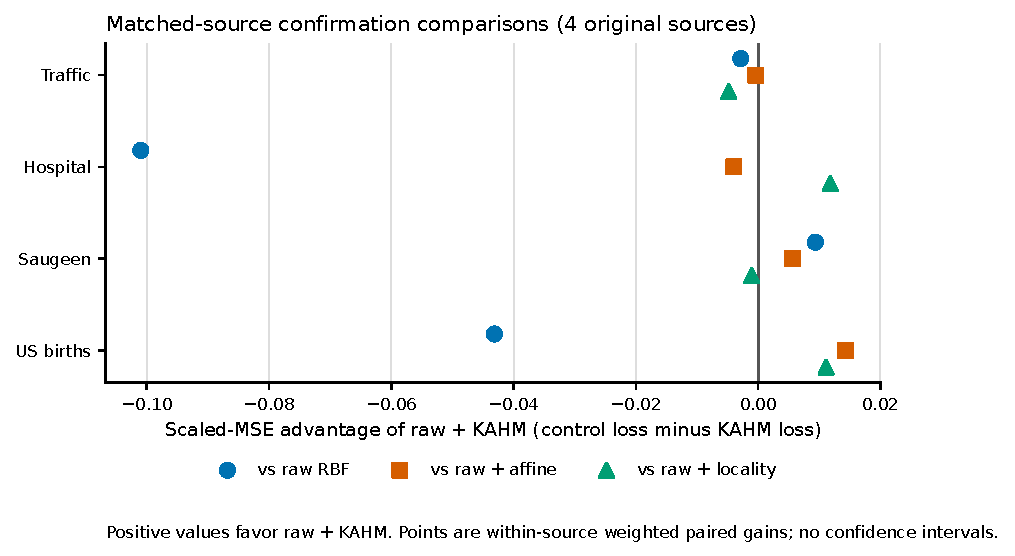
\includegraphics[width=\linewidth]{generated/natural/figures/source_gains.pdf}
\caption{Within-source confirmation comparisons. Positive differences favor
raw plus KAHM. Points compare the same hierarchically weighted source means;
no window-level uncertainty intervals are inferred. The small KAHM differences
against structural controls change sign across sources.}\label{fig:source-gains}
\end{figure}
\begin{figure}[t]
\centering
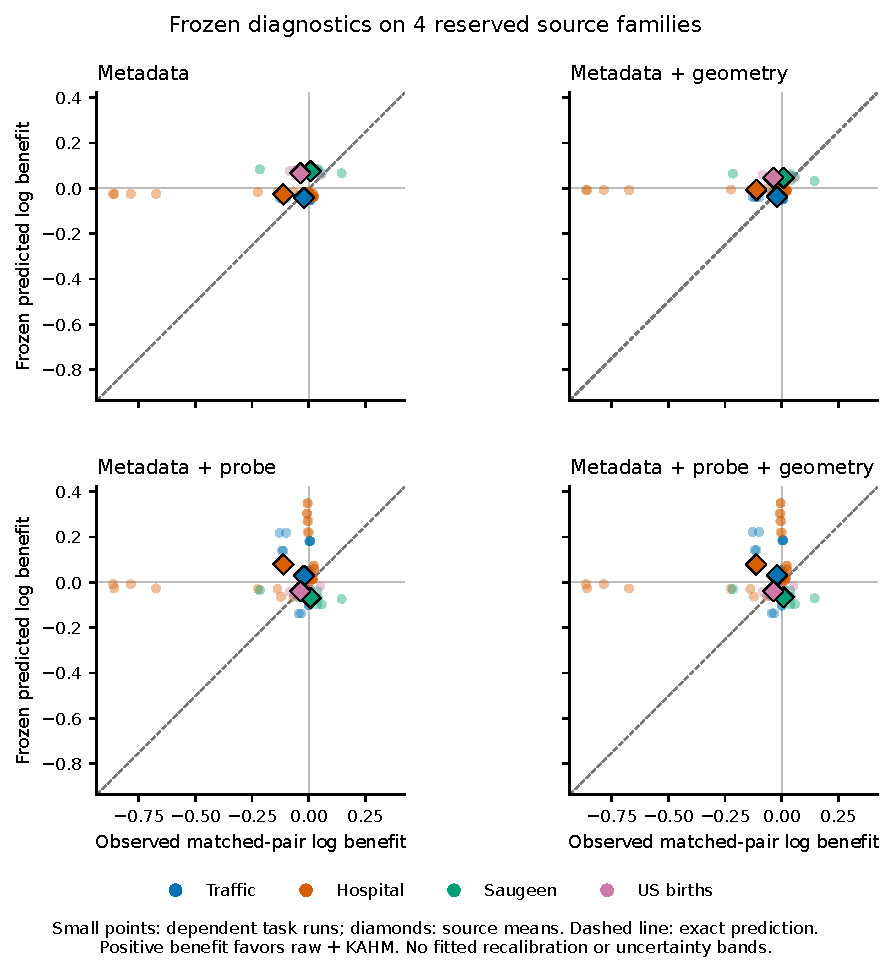
\includegraphics[width=0.92\linewidth]{generated/natural/figures/diagnostic_predictions.pdf}
\caption{Observed versus frozen predicted log benefit. Points within a source
are dependent task runs, and diamonds are source means. No recalibration is
fitted on confirmation. Similar decisions can coexist with different estimated
benefit magnitudes.}\label{fig:diagnostic-predictions}
\end{figure}
\FloatBarrier
{\small\setlength{\tabcolsep}{4pt}
\begin{longtable}{lrrrrr}
\caption{Development scaled MSE by original source family. The final column gives equal-source aggregation; source columns retain the declared within-source weights. Development diagnostics use leave-one-source-family-out fits; confirmation diagnostics use the frozen development fit. Always-policy rows duplicate their corresponding standalone methods deliberately.}\label{tab:source-development-loss}\\
\toprule
Method or policy & FRED-MD & NN5 & Tourism & Electricity & Equal-source \\
\midrule
\endfirsthead
\toprule
Method or policy & FRED-MD & NN5 & Tourism & Electricity & Equal-source \\
\midrule
\endhead
Raw ridge & 0.5601 & 0.8584 & 2.865 & 0.4243 & 1.177 \\
Raw RBF & 10.46 & 0.7552 & 3.476 & 0.4388 & 3.783 \\
Affine local & 2.548 & 0.8795 & 3.769 & 0.4535 & 1.912 \\
Locality local & 23.83 & 0.8148 & 3.778 & 0.4112 & 7.209 \\
KAHM local & 12.23 & 0.9163 & 3.636 & 0.4525 & 4.309 \\
Raw + affine & 1.409 & 0.7614 & 3.172 & 0.4481 & 1.448 \\
Raw + locality & 10.18 & 0.7474 & 3.046 & 0.4418 & 3.603 \\
Raw + KAHM & 4.254 & 0.7704 & 3.229 & 0.4539 & 2.177 \\
Seasonal naive & 2.269 & 1.089 & 2.982 & 0.5507 & 1.723 \\
Holt & 0.2409 & 1.358 & 8.228 & 0.6984 & 2.631 \\
Histogram boosting & 34.02 & 0.8032 & 4.786 & 0.4404 & 10.01 \\
MLP & 1.022 & 0.8475 & 2.77 & 0.4715 & 1.278 \\
Always raw & 10.46 & 0.7552 & 3.476 & 0.4388 & 3.783 \\
Always raw + KAHM & 4.254 & 0.7704 & 3.229 & 0.4539 & 2.177 \\
Validation: matched pair & 5.267 & 0.7335 & 3.229 & 0.4415 & 2.418 \\
Validation: raw portfolio & 0.2409 & 0.8021 & 3.014 & 0.4528 & 1.127 \\
Validation: KAHM family & 4.104 & 0.7792 & 3.223 & 0.4572 & 2.141 \\
Validation: full portfolio & 0.2409 & 0.8052 & 3.092 & 0.4675 & 1.152 \\
Cheap probe & 5.106 & 0.742 & 3.25 & 0.4217 & 2.38 \\
Metadata & 4.254 & 0.7704 & 3.229 & 0.4539 & 2.177 \\
Metadata + geometry & 4.254 & 0.7704 & 3.394 & 0.4539 & 2.218 \\
Metadata + probe & 4.157 & 0.759 & 3.338 & 0.4342 & 2.172 \\
Metadata + probe + geometry & 4.215 & 0.7704 & 3.338 & 0.4342 & 2.189 \\
\bottomrule
\end{longtable}
}

{\small\setlength{\tabcolsep}{4pt}
\begin{longtable}{lrrrrr}
\caption{Development warm-library wall seconds by original source family. The final column gives equal-source aggregation; source columns retain the declared within-source weights. Development diagnostics use leave-one-source-family-out fits; confirmation diagnostics use the frozen development fit. Always-policy rows duplicate their corresponding standalone methods deliberately.}\label{tab:source-development-cost}\\
\toprule
Method or policy & FRED-MD & NN5 & Tourism & Electricity & Equal-source \\
\midrule
\endfirsthead
\toprule
Method or policy & FRED-MD & NN5 & Tourism & Electricity & Equal-source \\
\midrule
\endhead
Raw ridge & 0.3731 & 0.1631 & 0.1888 & 0.1873 & 0.2281 \\
Raw RBF & 0.1929 & 0.1912 & 0.1834 & 0.1692 & 0.1842 \\
Affine local & 0.3285 & 0.2805 & 0.2983 & 0.2863 & 0.2984 \\
Locality local & 0.5431 & 0.29 & 0.2784 & 0.2649 & 0.3441 \\
KAHM local & 0.3705 & 0.3696 & 0.3735 & 0.3369 & 0.3626 \\
Raw + affine & 0.2923 & 0.2998 & 0.2979 & 0.288 & 0.2945 \\
Raw + locality & 0.3185 & 0.2967 & 0.2988 & 0.2533 & 0.2918 \\
Raw + KAHM & 0.4275 & 0.3807 & 0.3252 & 0.3024 & 0.3589 \\
Seasonal naive & 0.2125 & 0.177 & 0.1834 & 0.1878 & 0.1902 \\
Holt & 0.3224 & 0.42 & 0.3682 & 0.316 & 0.3567 \\
Histogram boosting & 3.086 & 4.954 & 1.729 & 1.819 & 2.897 \\
MLP & 1.278 & 0.9551 & 0.8521 & 0.5508 & 0.9089 \\
Always raw & 0.1929 & 0.1912 & 0.1834 & 0.1692 & 0.1842 \\
Always raw + KAHM & 0.4275 & 0.3807 & 0.3252 & 0.3024 & 0.3589 \\
Validation: matched pair & 0.5562 & 0.5313 & 0.4929 & 0.4301 & 0.5026 \\
Validation: raw portfolio & 4.066 & 5.306 & 2.641 & 2.719 & 3.683 \\
Validation: KAHM family & 0.692 & 0.6568 & 0.6115 & 0.5511 & 0.6278 \\
Validation: full portfolio & 5.861 & 6.513 & 4.138 & 4.075 & 5.147 \\
Cheap probe & 0.4739 & 0.4615 & 0.4004 & 0.3328 & 0.4172 \\
Metadata & 0.4284 & 0.3815 & 0.3258 & 0.3031 & 0.3597 \\
Metadata + geometry & 0.5195 & 0.465 & 0.3474 & 0.3744 & 0.4266 \\
Metadata + probe & 0.5029 & 0.474 & 0.2891 & 0.3411 & 0.4018 \\
Metadata + probe + geometry & 0.5284 & 0.4828 & 0.2891 & 0.341 & 0.4103 \\
\bottomrule
\end{longtable}
}

{\small\setlength{\tabcolsep}{4pt}
\begin{longtable}{lrrrrr}
\caption{Confirmation scaled MSE by original source family. The final column gives equal-source aggregation; source columns retain the declared within-source weights. Development diagnostics use leave-one-source-family-out fits; confirmation diagnostics use the frozen development fit. Always-policy rows duplicate their corresponding standalone methods deliberately.}\label{tab:source-confirmation-loss}\\
\toprule
Method or policy & Traffic & Hospital & Saugeen & US births & Equal-source \\
\midrule
\endfirsthead
\toprule
Method or policy & Traffic & Hospital & Saugeen & US births & Equal-source \\
\midrule
\endhead
Raw ridge & 0.5737 & 0.8461 & 0.522 & 1.177 & 0.7798 \\
Raw RBF & 0.5739 & 0.8228 & 0.6106 & 1.223 & 0.8075 \\
Affine local & 0.5796 & 0.928 & 0.6462 & 1.626 & 0.9449 \\
Locality local & 0.5719 & 0.7702 & 0.6504 & 1.593 & 0.8964 \\
KAHM local & 0.5775 & 0.9029 & 0.6652 & 1.596 & 0.9354 \\
Raw + affine & 0.5764 & 0.9198 & 0.6068 & 1.28 & 0.8458 \\
Raw + locality & 0.572 & 0.9356 & 0.6002 & 1.277 & 0.8462 \\
Raw + KAHM & 0.5768 & 0.9238 & 0.6012 & 1.266 & 0.8419 \\
Seasonal naive & 0.6484 & 0.7848 & 1.023 & 1.743 & 1.05 \\
Holt & 0.6842 & 1.003 & 0.6079 & 7.197 & 2.373 \\
Histogram boosting & 0.6524 & 1.025 & 0.5386 & 1.606 & 0.9555 \\
MLP & 0.6811 & 1.15 & 0.5365 & 1.147 & 0.8785 \\
Always raw & 0.5739 & 0.8228 & 0.6106 & 1.223 & 0.8075 \\
Always raw + KAHM & 0.5768 & 0.9238 & 0.6012 & 1.266 & 0.8419 \\
Validation: matched pair & 0.5738 & 0.8236 & 0.6042 & 1.237 & 0.8097 \\
Validation: raw portfolio & 0.6087 & 1.116 & 0.5639 & 1.167 & 0.8639 \\
Validation: KAHM family & 0.577 & 0.9182 & 0.6012 & 1.266 & 0.8406 \\
Validation: full portfolio & 0.6122 & 1.099 & 0.5695 & 1.225 & 0.8764 \\
Cheap probe & 0.5761 & 0.8211 & 0.6253 & 1.235 & 0.8143 \\
Metadata & 0.5739 & 0.8228 & 0.6012 & 1.266 & 0.816 \\
Metadata + geometry & 0.5739 & 0.8228 & 0.6012 & 1.266 & 0.816 \\
Metadata + probe & 0.5761 & 0.8189 & 0.6106 & 1.223 & 0.8071 \\
Metadata + probe + geometry & 0.5761 & 0.8189 & 0.6106 & 1.223 & 0.8071 \\
\bottomrule
\end{longtable}
}

{\small\setlength{\tabcolsep}{4pt}
\begin{longtable}{lrrrrr}
\caption{Confirmation warm-library wall seconds by original source family. The final column gives equal-source aggregation; source columns retain the declared within-source weights. Development diagnostics use leave-one-source-family-out fits; confirmation diagnostics use the frozen development fit. Always-policy rows duplicate their corresponding standalone methods deliberately.}\label{tab:source-confirmation-cost}\\
\toprule
Method or policy & Traffic & Hospital & Saugeen & US births & Equal-source \\
\midrule
\endfirsthead
\toprule
Method or policy & Traffic & Hospital & Saugeen & US births & Equal-source \\
\midrule
\endhead
Raw ridge & 0.1454 & 0.1959 & 0.1905 & 0.2204 & 0.188 \\
Raw RBF & 0.1644 & 0.1636 & 0.1693 & 0.1779 & 0.1688 \\
Affine local & 0.2424 & 0.2732 & 0.4038 & 1.082 & 0.5002 \\
Locality local & 0.2311 & 0.254 & 0.4021 & 0.2721 & 0.2898 \\
KAHM local & 0.2579 & 0.2764 & 0.3496 & 0.4035 & 0.3218 \\
Raw + affine & 0.3969 & 0.2809 & 0.354 & 0.3199 & 0.3379 \\
Raw + locality & 0.2223 & 0.2752 & 0.3166 & 0.3022 & 0.2791 \\
Raw + KAHM & 0.2674 & 0.4235 & 0.4676 & 0.3911 & 0.3874 \\
Seasonal naive & 0.1551 & 0.164 & 0.1874 & 0.1393 & 0.1614 \\
Holt & 0.2759 & 0.3535 & 0.4118 & 0.3386 & 0.3449 \\
Histogram boosting & 1.774 & 1.39 & 17.59 & 14.89 & 8.91 \\
MLP & 0.4046 & 0.392 & 2.264 & 2.79 & 1.463 \\
Always raw & 0.1644 & 0.1636 & 0.1693 & 0.1779 & 0.1688 \\
Always raw + KAHM & 0.2674 & 0.4235 & 0.4676 & 0.3911 & 0.3874 \\
Validation: matched pair & 0.3909 & 0.5408 & 0.5273 & 0.4656 & 0.4812 \\
Validation: raw portfolio & 2.276 & 2.19 & 15.94 & 12.95 & 8.338 \\
Validation: KAHM family & 0.4622 & 0.6403 & 0.7116 & 0.6829 & 0.6242 \\
Validation: full portfolio & 3.595 & 3.661 & 17.63 & 14.9 & 9.948 \\
Cheap probe & 0.3029 & 0.2768 & 0.4534 & 0.3531 & 0.3465 \\
Metadata & 0.1651 & 0.1644 & 0.4686 & 0.3923 & 0.2976 \\
Metadata + geometry & 0.2216 & 0.2212 & 0.5797 & 0.4555 & 0.3695 \\
Metadata + probe & 0.2958 & 0.457 & 0.3033 & 0.2673 & 0.3309 \\
Metadata + probe + geometry & 0.2958 & 0.457 & 0.3033 & 0.2673 & 0.3309 \\
\bottomrule
\end{longtable}
}

{\small\setlength{\tabcolsep}{4pt}
\begin{longtable}{lrrrr}
\caption{Development capacity comparison. Each capacity changes specified training-window and model-size caps; it is not an equal-time budget. Values are equal-source weighted and retain all prescribed context--horizon settings and seeds.}\label{tab:capacity-development}\\
\toprule
Method or policy & medium MSE & medium wall (s) & small MSE & small wall (s) \\
\midrule
\endfirsthead
\toprule
Method or policy & medium MSE & medium wall (s) & small MSE & small wall (s) \\
\midrule
\endhead
Raw ridge & 1.177 & 0.28 & 1.177 & 0.1761 \\
Raw RBF & 4.582 & 0.1846 & 2.984 & 0.1838 \\
Affine local & 1.989 & 0.3292 & 1.836 & 0.2676 \\
Locality local & 8.238 & 0.4065 & 6.18 & 0.2817 \\
KAHM local & 3.855 & 0.3779 & 4.763 & 0.3473 \\
Raw + affine & 1.394 & 0.3071 & 1.501 & 0.282 \\
Raw + locality & 3.879 & 0.3038 & 3.327 & 0.2798 \\
Raw + KAHM & 2.332 & 0.3819 & 2.022 & 0.3359 \\
Seasonal naive & 1.723 & 0.2078 & 1.723 & 0.1725 \\
Holt & 2.631 & 0.345 & 2.632 & 0.3683 \\
Histogram boosting & 9.795 & 3.468 & 10.23 & 2.326 \\
MLP & 1.253 & 1.108 & 1.302 & 0.7098 \\
Always raw & 4.582 & 0.1846 & 2.984 & 0.1838 \\
Always raw + KAHM & 2.332 & 0.3819 & 2.022 & 0.3359 \\
Validation: matched pair & 2.342 & 0.5295 & 2.493 & 0.4758 \\
Validation: raw portfolio & 1.128 & 4.223 & 1.127 & 3.142 \\
Validation: KAHM family & 2.261 & 0.6594 & 2.021 & 0.5963 \\
Validation: full portfolio & 1.137 & 5.805 & 1.166 & 4.488 \\
Cheap probe & 2.297 & 0.4321 & 2.463 & 0.4022 \\
Metadata & 2.332 & 0.3828 & 2.022 & 0.3367 \\
Metadata + geometry & 2.364 & 0.4492 & 2.072 & 0.404 \\
Metadata + probe & 2.337 & 0.419 & 2.007 & 0.3846 \\
Metadata + probe + geometry & 2.348 & 0.4327 & 2.03 & 0.388 \\
\bottomrule
\end{longtable}
}

{\small\setlength{\tabcolsep}{4pt}
\begin{longtable}{lrrrr}
\caption{Confirmation capacity comparison. Each capacity changes specified training-window and model-size caps; it is not an equal-time budget. Values are equal-source weighted and retain all prescribed context--horizon settings and seeds.}\label{tab:capacity-confirmation}\\
\toprule
Method or policy & medium MSE & medium wall (s) & small MSE & small wall (s) \\
\midrule
\endfirsthead
\toprule
Method or policy & medium MSE & medium wall (s) & small MSE & small wall (s) \\
\midrule
\endhead
Raw ridge & 0.7635 & 0.1561 & 0.7961 & 0.2199 \\
Raw RBF & 0.7767 & 0.1719 & 0.8383 & 0.1657 \\
Affine local & 0.916 & 0.3088 & 0.9738 & 0.6917 \\
Locality local & 0.8908 & 0.3176 & 0.902 & 0.2621 \\
KAHM local & 0.9243 & 0.334 & 0.9466 & 0.3097 \\
Raw + affine & 0.8233 & 0.3859 & 0.8684 & 0.2899 \\
Raw + locality & 0.8363 & 0.2831 & 0.8561 & 0.275 \\
Raw + KAHM & 0.8288 & 0.3732 & 0.8551 & 0.4016 \\
Seasonal naive & 1.05 & 0.1621 & 1.05 & 0.1607 \\
Holt & 2.373 & 0.333 & 2.373 & 0.3569 \\
Histogram boosting & 0.9215 & 12.73 & 0.9896 & 5.086 \\
MLP & 0.8712 & 1.956 & 0.8859 & 0.9695 \\
Always raw & 0.7767 & 0.1719 & 0.8383 & 0.1657 \\
Always raw + KAHM & 0.8288 & 0.3732 & 0.8551 & 0.4016 \\
Validation: matched pair & 0.7847 & 0.4538 & 0.8347 & 0.5085 \\
Validation: raw portfolio & 0.8404 & 11.6 & 0.8874 & 5.074 \\
Validation: KAHM family & 0.8281 & 0.6116 & 0.8531 & 0.6369 \\
Validation: full portfolio & 0.8541 & 12.98 & 0.8987 & 6.918 \\
Cheap probe & 0.7943 & 0.3749 & 0.8343 & 0.3182 \\
Metadata & 0.8009 & 0.3187 & 0.8311 & 0.2764 \\
Metadata + geometry & 0.8009 & 0.3779 & 0.8311 & 0.3611 \\
Metadata + probe & 0.7765 & 0.2805 & 0.8377 & 0.3812 \\
Metadata + probe + geometry & 0.7765 & 0.2805 & 0.8377 & 0.3812 \\
\bottomrule
\end{longtable}
}

{\small\setlength{\tabcolsep}{4pt}
\begin{longtable}{lrrrr}
\caption{Estimated-benefit diagnostics with frozen hierarchical weights. These are descriptive log-benefit prediction errors and classification accuracies; they are not calibrated probabilities or interval coverage. No recalibration is fitted on confirmation data.}\label{tab:diagnostic-calibration}\\
\toprule
Diagnostic & Log RMSE & Log bias & Sign (\%) & 5\% class (\%) \\
\midrule
\endfirsthead
\toprule
Diagnostic & Log RMSE & Log bias & Sign (\%) & 5\% class (\%) \\
\midrule
\endhead
Development: Metadata & 1.035 & 0.01412 & 57 & 49.2 \\
Development: Metadata + geometry & 1.037 & 0.03491 & 47.7 & 43 \\
Development: Metadata + probe & 1.012 & 0.03064 & 52.3 & 53.9 \\
Development: Metadata + probe + geometry & 1.02 & 0.05091 & 50.8 & 43 \\
Confirmation: Metadata & 0.1643 & 0.05835 & 55.5 & 59.4 \\
Confirmation: Metadata + geometry & 0.1612 & 0.05269 & 55.5 & 75 \\
Confirmation: Metadata + probe & 0.1845 & 0.04069 & 58.6 & 73.4 \\
Confirmation: Metadata + probe + geometry & 0.1847 & 0.04196 & 58.6 & 71.9 \\
\bottomrule
\end{longtable}
}

{\small\setlength{\tabcolsep}{4pt}
\begin{longtable}{lrrrr}
\caption{One-off diagnostic development costs. Acquisition sums the union of both matched predictors' complete search/final nodes and each variant's metadata/probe/geometry dependencies within every development task. Summing standalone tasks can conservatively repeat preparation across seeds/tasks. Acquire and total denote wall time; CPU covers acquisition. The rows share development labels and some features, so their costs are not additive. Ridge fitting is measured separately; no deployment-count amortization is assumed.}\label{tab:offline-costs}\\
\toprule
Variant & Acquire (s) & CPU (s) & Ridge (ms) & Total (s) \\
\midrule
\endfirsthead
\toprule
Variant & Acquire (s) & CPU (s) & Ridge (ms) & Total (s) \\
\midrule
\endhead
Metadata & 68.49 & 68.45 & 6.657 & 68.5 \\
Metadata + geometry & 78.6 & 78.56 & 10.04 & 78.61 \\
Metadata + probe & 80.83 & 80.79 & 9.035 & 80.84 \\
Metadata + probe + geometry & 80.83 & 80.79 & 6.146 & 80.84 \\
\bottomrule
\end{longtable}
}

{\small\setlength{\tabcolsep}{4pt}
\begin{longtable}{lrrrrrr}
\caption{Frozen development-only standardization and ridge coefficients, rounded for display. G denotes geometry and P the cheap probe. An absent feature is shown by a dash. Predictions use the unrounded values in the frozen diagnostic JSON and the fixed zero decision threshold.}\label{tab:diagnostic-coefficients}\\
\toprule
Feature & Mean & Scale & Meta & Meta+G & Meta+P & Meta+P+G \\
\midrule
\endfirsthead
\toprule
Feature & Mean & Scale & Meta & Meta+G & Meta+P & Meta+P+G \\
\midrule
\endhead
Intercept & -- & -- & 0.023966 & 0.023966 & 0.023966 & 0.023966 \\
log(1 + training windows) & 5.1417 & 0.66192 & 0.017096 & 0.013047 & -0.0099182 & -0.0089504 \\
log(1 + horizon/history) & 0.23442 & 0.019538 & -0.012299 & -0.013178 & -0.0043432 & -0.0045441 \\
Lag-one autocorrelation & 0.7189 & 0.24263 & 0.0069415 & 0.001093 & -0.014509 & -0.012806 \\
KAHM gate entropy & 0.074168 & 0.063288 & -- & -0.010312 & -- & -0.0026401 \\
log(1 + affine residual) & 0.18213 & 0.12986 & -- & -0.013232 & -- & 0.0063025 \\
Probe log-loss ratio & 0.25347 & 0.67921 & -- & -- & 0.14611 & 0.1467 \\
\bottomrule
\end{longtable}
}

{\small\setlength{\tabcolsep}{4pt}
\begin{longtable}{lrrrrr}
\caption{Recorded fitting behavior. Search and selected-refit warning events are separated. Counts describe task fits, which include dependent seeds and settings. Warned counts fits with recorded warnings; at cap counts selected refits reaching the recorded iteration limit. Full warning text is retained in the JSON report. No warning-triggered post hoc retuning is applied.}\label{tab:fit-warnings}\\
\toprule
Method & Fits & Warned & Search & Refit & At cap \\
\midrule
\endfirsthead
\toprule
Method & Fits & Warned & Search & Refit & At cap \\
\midrule
\endhead
Development: Raw ridge & 128 & 0 & 0 & 0 & 0 \\
Development: Raw RBF & 128 & 0 & 0 & 0 & 0 \\
Development: Affine local & 128 & 0 & 0 & 0 & 0 \\
Development: Locality local & 128 & 0 & 0 & 0 & 0 \\
Development: KAHM local & 128 & 0 & 0 & 0 & 0 \\
Development: Raw + affine & 128 & 0 & 0 & 0 & 0 \\
Development: Raw + locality & 128 & 0 & 0 & 0 & 0 \\
Development: Raw + KAHM & 128 & 0 & 0 & 0 & 0 \\
Development: Seasonal naive & 128 & 0 & 0 & 0 & 0 \\
Development: Holt & 128 & 0 & 0 & 0 & 0 \\
Development: Histogram boosting & 128 & 0 & 0 & 0 & 0 \\
Development: MLP & 128 & 128 & 232 & 105 & 105 \\
Confirmation: Raw ridge & 80 & 0 & 0 & 0 & 0 \\
Confirmation: Raw RBF & 80 & 0 & 0 & 0 & 0 \\
Confirmation: Affine local & 80 & 0 & 0 & 0 & 0 \\
Confirmation: Locality local & 80 & 0 & 0 & 0 & 0 \\
Confirmation: KAHM local & 80 & 0 & 0 & 0 & 0 \\
Confirmation: Raw + affine & 80 & 0 & 0 & 0 & 0 \\
Confirmation: Raw + locality & 80 & 0 & 0 & 0 & 0 \\
Confirmation: Raw + KAHM & 80 & 0 & 0 & 0 & 0 \\
Confirmation: Seasonal naive & 80 & 0 & 0 & 0 & 0 \\
Confirmation: Holt & 80 & 0 & 0 & 0 & 0 \\
Confirmation: Histogram boosting & 80 & 0 & 0 & 0 & 0 \\
Confirmation: MLP & 80 & 79 & 137 & 68 & 68 \\
\bottomrule
\end{longtable}
}

{\small\setlength{\tabcolsep}{4pt}
\begin{longtable}{lrrrrr}
\caption{Selection at numerical search-grid endpoints. Counts are descriptive; a two-point grid necessarily chooses an endpoint. These observations do not establish the benefit of a larger grid, and confirmation outcomes are not used to retune any method.}\label{tab:grid-boundaries}\\
\toprule
Method & Parameter & Choices & Lower & Upper & Declared grid \\
\midrule
\endfirsthead
\toprule
Method & Parameter & Choices & Lower & Upper & Declared grid \\
\midrule
\endhead
Development: Raw ridge & alpha & 128 & 84 & 4 & 0.01,1,100 \\
Development: Raw RBF & alpha & 128 & 35 & 4 & 0.01,1,100 \\
Development: Affine local & alpha & 128 & 45 & 8 & 0.01,1,100 \\
Development: Locality local & alpha & 128 & 35 & 9 & 0.01,1,100 \\
Development: KAHM local & alpha & 128 & 51 & 7 & 0.01,1,100 \\
Development: Raw + affine & alpha & 128 & 32 & 4 & 0.01,1,100 \\
Development: Raw + locality & alpha & 128 & 25 & 5 & 0.01,1,100 \\
Development: Raw + KAHM & alpha & 128 & 30 & 4 & 0.01,1,100 \\
Development: Histogram boosting & regularization & 128 & 78 & 50 & 0.01,1 \\
Development: MLP & regularization & 128 & 26 & 102 & 0.01,1 \\
Confirmation: Raw ridge & alpha & 80 & 20 & 56 & 0.01,1,100 \\
Confirmation: Raw RBF & alpha & 80 & 13 & 56 & 0.01,1,100 \\
Confirmation: Affine local & alpha & 80 & 9 & 58 & 0.01,1,100 \\
Confirmation: Locality local & alpha & 80 & 9 & 60 & 0.01,1,100 \\
Confirmation: KAHM local & alpha & 80 & 8 & 59 & 0.01,1,100 \\
Confirmation: Raw + affine & alpha & 80 & 12 & 59 & 0.01,1,100 \\
Confirmation: Raw + locality & alpha & 80 & 12 & 61 & 0.01,1,100 \\
Confirmation: Raw + KAHM & alpha & 80 & 12 & 60 & 0.01,1,100 \\
Confirmation: Histogram boosting & regularization & 80 & 34 & 46 & 0.01,1 \\
Confirmation: MLP & regularization & 80 & 5 & 75 & 0.01,1 \\
\bottomrule
\end{longtable}
}


\section{Reconstructing the numerical evidence}\label{app:reproduction}
The supplement has separate controlled and natural forecasting entry points,
plus an integrated review manifest. Its README gives commands to verify the
packaged bytes, independently reconstruct archived losses, replay diagnostics,
regenerate paper assets, and compile the anonymous manuscript. The scientific
implementations and original outcome records remain unchanged. Documentation
and review manifests added after execution are labeled as such; they are not
new pre-outcome registrations or external timing attestations.

For the controlled study, full regeneration generates new working files from
the archived configurations and retained seed streams, while compact-record
auditing checks the existing outcomes. These operations reproduce the same
evidence rather than add independent repetitions. The natural study retains
both stage freezes, all 208 completed runs, prepared windows, prediction arrays,
source snapshot hashes, and original environment/cost records. Its offline
audit checks the complete twelve-method roster, targets and forecast origins,
all 2,496 losses, and frozen diagnostic outcomes without refitting forecasting
models. Replaying a small diagnostic regression can generate different
microsecond timing measurements; original measured resource records remain
separate from those replay timings.

All eight natural dataset snapshots retain their attribution and licenses.
The inherited implementation and template retain required third-party notices.
Anonymization omits named study overviews and author-linked locators while
preserving the scientific dependency bytes and identifying the scope of the
review export. The separately supplied related certificate manuscript is
background for the scope comparison, not a source of additional experimental
replications or a certificate for the present fitted predictors.

\FloatBarrier
\section{Bounded sensitivity to geometry scaling}\label{app:scaling}
\subsection{Execution boundary and estimand}
The original experiments in Sections~\ref{c:sec:capacity} and~\ref{sec:natural}
use training z-score geometry scaling. The sensitivity analysis was specified
after inspecting those experiments. Its protocol and execution sources were
published and hashed before the sensitivity fits, and both fixed scaler arms
were retained. This ordering prevents choosing the sensitivity cells after
their outcomes; it does not make the reused natural sources or synthetic draws
fresh confirmation evidence. No adoption diagnostic or best-scaler selection
rule was refitted.

The intervention replaces only the geometry input scaler by
\[
 z_j(x)=2\frac{x_j-m_j}{M_j-m_j}-1,
 \qquad m_j=\min_{i\in\mathcal T}x_{ij},\quad
 M_j=\max_{i\in\mathcal T}x_{ij}.
\]
The fitting set $\mathcal T$ is the exact training input set for that fit,
before its geometry subsample. Coordinates with exactly zero training range
are mapped to zero for every geometry query, matching the historical
implementation. Validation and test queries are not clipped; values can
exceed $[-1,1]$. Raw references and the raw skip retain their original training
standardization. Feature standardization, target standardization, loss scales,
forecast horizons, data and model seeds, hyperparameter grids, query arithmetic,
and the controlled study's known-support output clipping are unchanged.

Changing the scaler inside the geometry pipeline matters. It can alter
partitions, truncated principal directions, absolute reconstruction distances,
and angles relative to the origin. The historical kernel fit also uses a
regularization level depending on the squared reference-coordinate magnitude.
Downstream feature standardization does not reverse these nonlinear changes.
By contrast, a nonconstant coordinate's positive affine min--max transform
followed by refitted z-score standardization cancels in exact arithmetic
when threshold-based scale fallbacks are inactive:
$[(a x+b)-(a\mu+b)]/(a\sigma)=(x-\mu)/\sigma$ for $a>0$.
The experiment therefore replaces the geometry scaler itself.

\subsection{Natural-source execution}
All 208 original configurations are reused: 128 on the original development
sources and 80 on the four formerly reserved sources. Each configuration runs
raw plus affine, raw plus locality, and raw plus KAHM under both scalers,
together with unchanged raw ridge and raw RBF references: 1,664 standalone
method runs. The local-only natural architectures and the frozen benefit
diagnostic are outside this bounded sensitivity. Each fixed arm uses the
original validation-only alpha selection; the selected model is then refitted
on the original admissible pretest windows. Its scaler is fitted anew on that
refit set, without test observations.

The primary descriptive contrast is min--max minus standard raw-plus-KAHM
scaled MSE on the four formerly reserved source families. Each mean uses the
original source/series/regime/capacity/seed hierarchy. The original development
sources are reported separately. Source-wise and leave-one-source-out results
describe heterogeneity; neither seeds nor overlapping histories supply
additional independent source families. There are no new confirmatory
$p$-values or simultaneous superiority claims.

Methods execute serially in one benchmark worker with one BLAS thread;
method order is shuffled deterministically by task identity, independently
of outcomes. New warm-library costs include alpha search, selection cleanup,
selected refit, prediction, and serialization. Current data loading,
launch-to-result wall time, and the additional sensitivity diagnostics are
recorded separately; the original source preparation is reused, rather than
freshly timed. The launch-to-result field includes child execution and communication, rather
than isolating startup overhead. The inherited import timer starts after some
adapter dependencies have loaded, so it does not measure full cold startup.
New cost comparisons use references remeasured in this execution. They must not
be formed by dividing a new method time by an old archived baseline time.

\subsection{Controlled execution}
The sensitivity recreates the exact 24 complete phase-four data/fit draws for
each of autoregression, Van der Pol, and Duffing, at 64 and 256 landmarks.
All four original representations are retained under both geometry scalers:
raw, affine local coordinates, KAHM local coordinates, and KAHM scores.
An explicitly added locality-coordinate control uses the historical
native-affine locality gates with the same local principal coordinates.
Thus 72 paired jobs produce 1,440 head fits. The raw representation is
identical across scaler arms. The original target bounds and validation
selection rules remain in force.

For each law/capacity cell, the unit of paired dispersion is a complete
data/fit draw. Episode losses and horizon errors are retained but are not
counted as additional independent fitted-method repetitions. The analysis
reports means and paired standard deviations/standard errors descriptively;
the original contrast families' confidence statements are not extended to
these post-hoc comparisons. Controlled banks are shared across their
representations, so controlled execution times are not standalone deployment
cost estimates.

\subsection{Numerical verification and retained evidence}
The standard natural arms and fixed references are checked against all 1,040
corresponding task--method prediction arrays and selected hyperparameters.
All 576 original
standard controlled method/capacity fits are checked against archived
predictions, losses, and selected hyperparameters; 144 controlled raw
cross-scaler pairs are checked for equality. The separate audit reconstructs
the new natural losses from per-origin forecasts and all controlled losses
from the full saved prediction arrays before compact export.

The review supplement retains every natural sensitivity forecast and all
controlled per-episode losses, execution records, selected settings, scaler
statistics, out-of-range diagnostics, and file digests. Full controlled
predictions and fitted banks are regenerated by the supplied runner; their
pre-export verification is recorded in the retained full-prediction audit.
Replaying the compact controlled losses is distinguished from independently
recreating and checking those full prediction arrays. The original studies'
scientific sources, freezes, and outcomes remain unchanged.

\subsection{Natural heterogeneity and costs}
Table~\ref{tab:scaling-development} keeps the original development outcomes
separate. KAHM's development loss increases by 7.70\%; the source changes
are $-1.99$\% on Electricity, $+2.06$\% on NN5, $-5.20$\% on Tourism,
and $+19.54$\% on FRED-MD. Removing FRED-MD changes the aggregate scaler
effect to a 3.62\% reduction. Neither development aggregation should be
used to select a scaler on those already inspected outcomes.
Table~\ref{tab:scaling-sources} reports both original role groups, and
Tables~\ref{tab:scaling-all-sources-development}
and~\ref{tab:scaling-all-sources-confirmation} retain every fixed method.

% Generated by scaling_sensitivity/report.py from analysis/summary.json.
\begin{table}[t]
\centering
\small
\begin{tabular}{lrrr}
\toprule
Method & Standard MSE & Min--max MSE & Change (\%) \\
\midrule
Raw ridge & 1.1769 & 1.1769 & fixed \\
Raw RBF & 3.7827 & 3.7827 & fixed \\
Raw + affine & 1.4475 & 1.3306 & -8.08 \\
Raw + locality & 3.6030 & 3.3309 & -7.55 \\
Raw + KAHM & 2.1768 & 2.3444 & +7.70 \\
\bottomrule
\end{tabular}
\caption{The same fixed sensitivity comparison on the four original development sources. Their outcomes remain separate from the formerly reserved sources. Scaled MSE uses the original equal-source hierarchy; change is min--max versus standard in percent. Raw references are fixed, and no scaler is selected from these test outcomes.}
\label{tab:scaling-development}
\end{table}

% Generated by scaling_sensitivity/report.py from analysis/summary.json.
\begin{table}[t]
\centering
\scriptsize
\begin{tabular}{lrrrrrr}
\toprule
Source & $K_s$ & $K_m$ & $\Delta\%$ & $R$ & $A_m$ & $L_m$ \\
\midrule
\multicolumn{7}{l}{\emph{Original development sources}} \\
Electricity & 0.4539 & 0.4448 & -1.99 & 0.4388 & 0.4584 & 0.4387 \\
NN5 & 0.7704 & 0.7863 & +2.06 & 0.7552 & 0.7824 & 0.7516 \\
Tourism & 3.2286 & 3.0606 & -5.20 & 3.4759 & 3.0768 & 3.0986 \\
FRED-MD & 4.2545 & 5.0857 & +19.54 & 10.4610 & 1.0050 & 9.0346 \\
\midrule
\multicolumn{7}{l}{\emph{Formerly reserved sources}} \\
Traffic & 0.5768 & 0.5759 & -0.15 & 0.5739 & 0.5750 & 0.5722 \\
Hospital & 0.9238 & 0.9158 & -0.86 & 0.8228 & 0.9157 & 0.8371 \\
Saugeen & 0.6012 & 0.6067 & +0.90 & 0.6106 & 0.6646 & 0.6773 \\
US births & 1.2659 & 1.2704 & +0.35 & 1.2228 & 1.2830 & 1.3085 \\
\bottomrule
\end{tabular}
\caption{Source-level scaling sensitivity. $K_s$ and $K_m$ denote raw + KAHM with standard and min--max geometry; $R$, $A_m$, and $L_m$ denote raw RBF, raw + min--max affine, and raw + min--max locality. Entries are original-hierarchy scaled MSE; $\Delta\% = 100(K_m/K_s-1)$. Original role labels identify the historical design, while every newly computed comparison is post-hoc.}
\label{tab:scaling-sources}
\end{table}

% Generated by scaling_sensitivity/report.py from analysis/summary.json.
\begin{table}[t]
\centering
\small
\begin{tabular}{lrrrr}
\toprule
Method / geometry scaler & Electricity & NN5 & Tourism & FRED-MD \\
\midrule
Raw ridge & 0.4243 & 0.8584 & 2.8648 & 0.5601 \\
Raw RBF & 0.4388 & 0.7552 & 3.4759 & 10.4610 \\
Raw + affine / std. & 0.4481 & 0.7614 & 3.1717 & 1.4090 \\
Raw + affine / min--max & 0.4584 & 0.7824 & 3.0768 & 1.0050 \\
Raw + locality / std. & 0.4418 & 0.7474 & 3.0458 & 10.1769 \\
Raw + locality / min--max & 0.4387 & 0.7516 & 3.0986 & 9.0346 \\
Raw + KAHM / std. & 0.4539 & 0.7704 & 3.2286 & 4.2545 \\
Raw + KAHM / min--max & 0.4448 & 0.7863 & 3.0606 & 5.0857 \\
\bottomrule
\end{tabular}
\caption{Every fixed sensitivity method on the original development sources. Entries are source-level scaled MSE using the original nested task weights. The two raw references retain their original standardization.}
\label{tab:scaling-all-sources-development}
\end{table}

% Generated by scaling_sensitivity/report.py from analysis/summary.json.
\begin{table}[t]
\centering
\small
\begin{tabular}{lrrrr}
\toprule
Method / geometry scaler & Traffic & Hospital & Saugeen & US births \\
\midrule
Raw ridge & 0.5737 & 0.8461 & 0.5220 & 1.1775 \\
Raw RBF & 0.5739 & 0.8228 & 0.6106 & 1.2228 \\
Raw + affine / std. & 0.5764 & 0.9198 & 0.6068 & 1.2802 \\
Raw + affine / min--max & 0.5750 & 0.9157 & 0.6646 & 1.2830 \\
Raw + locality / std. & 0.5720 & 0.9356 & 0.6002 & 1.2770 \\
Raw + locality / min--max & 0.5722 & 0.8371 & 0.6773 & 1.3085 \\
Raw + KAHM / std. & 0.5768 & 0.9238 & 0.6012 & 1.2659 \\
Raw + KAHM / min--max & 0.5759 & 0.9158 & 0.6067 & 1.2704 \\
\bottomrule
\end{tabular}
\caption{Every fixed sensitivity method on the formerly reserved sources. Entries are source-level scaled MSE using the original nested task weights. The two raw references retain their original standardization.}
\label{tab:scaling-all-sources-confirmation}
\end{table}

\FloatBarrier

The source-balanced fraction of test input coordinates outside the final
refit range is 3.77\% on the formerly reserved sources and 21.45\% on the
original development sources. The corresponding fractions of histories
with at least one such coordinate are 33.08\% and 49.26\%. The largest
absolute transformed test coordinate is 3.1990 and 1.8638, respectively.
No final natural refit has a constant input coordinate. These diagnostics
confirm that unclipped min--max scaling is distinct from enforcing bounded
query inputs; a clipped alternative was not tested.

Table~\ref{tab:scaling-costs} gives the new warm method stages.
The retained KAHM min--max Saugeen configuration with history 28, horizon 7,
medium capacity, and seed 17 takes 6.2914 seconds, including 4.7618 seconds
of search and 1.3632 seconds of cleanup. It is included at its original
hierarchical weight, without trimming or a timing-based rerun. The single
execution cannot distinguish algorithmic cost changes from runtime variation
with the precision of a separate repeated timing benchmark.

% Generated by scaling_sensitivity/report.py from analysis/summary.json.
\begin{table}[!htbp]
\centering
\scriptsize
\begin{tabular}{lrrrrrr}
\toprule
Method / geometry scaler & Search & Cleanup & Refit & Forecast & Serialize & Total \\
\midrule
Raw ridge & 0.0065 & 0.1770 & 0.0022 & 0.0001 & 0.0005 & 0.1863 \\
Raw RBF & 0.0136 & 0.1557 & 0.0062 & 0.0003 & 0.0005 & 0.1762 \\
Raw + affine / std. & 0.2316 & 0.1554 & 0.0530 & 0.0036 & 0.0021 & 0.4457 \\
Raw + affine / min--max & 0.0909 & 0.1639 & 0.0593 & 0.0025 & 0.0012 & 0.3178 \\
Raw + locality / std. & 0.0887 & 0.1671 & 0.0612 & 0.0022 & 0.0018 & 0.3210 \\
Raw + locality / min--max & 0.0825 & 0.1557 & 0.0672 & 0.0025 & 0.0029 & 0.3108 \\
Raw + KAHM / std. & 0.1162 & 0.1594 & 0.0939 & 0.0094 & 0.0015 & 0.3804 \\
Raw + KAHM / min--max & 0.2682 & 0.1934 & 0.0845 & 0.0084 & 0.0016 & 0.5561 \\
\bottomrule
\end{tabular}
\caption{Contemporaneous, source-balanced warm method times (seconds) on the four formerly reserved sources. Each method independently performs its alpha search, selected refit, prediction, serialization, and cleanup. These totals exclude reused data preparation, current input loading, process startup, and additional sensitivity audits. Launch-to-result and audit elapsed times are recorded separately; the recorded import interval covers only part of initialization. Every timing, including outliers, is retained. These single-execution observations are implementation-specific. Cost ratios use reference methods measured in this same execution.}
\label{tab:scaling-costs}
\end{table}

\FloatBarrier

\clearpage
\subsection{Complete controlled sensitivity}
Table~\ref{tab:scaling-controlled-all} includes all ten representation/scaler
arms in every law/capacity cell. KAHM local-coordinate mean error changes
by $-0.24/-0.32$\% on autoregression, $-0.18/+0.23$\% on Van der Pol,
and $-2.85/-7.35$\% on Duffing at 64/256 landmarks. The main mean rankings
are unchanged. The score-only KAHM representation is more sensitive on
Van der Pol, where min--max raises its error by 6.03\% and 4.78\%.
A secondary ordering consequently reverses at 256 landmarks: standardized
KAHM scores have mean MSE $1.0499\times10^{-3}$, below affine-local
$1.0780\times10^{-3}$, whereas their min--max errors are $1.1001\times10^{-3}$
and $1.0812\times10^{-3}$, respectively. The persistence claim concerns the
main KAHM-local versus raw/control comparisons, not every pair of methods.
The retained repetition-level CSVs supply all paired differences and
standard errors; the displayed standard deviations describe variability
and do not imply a new simultaneous confidence guarantee.

% Generated by scaling_sensitivity/report.py from analysis/summary.json.
\begingroup
\scriptsize
\setlength{\tabcolsep}{4pt}
\begin{longtable}{lrlrrr}
\caption{Every controlled sensitivity arm, including raw and KAHM scores. Each entry is mean MSE with between-repetition SD in parentheses, multiplied by $10^3$, over the same 24 complete draws. $\Delta$ is paired min--max-minus-standard mean difference; its parentheses contain paired SD. These are descriptive dispersions on reused draws, not confidence intervals. The raw arms are identical.}\label{tab:scaling-controlled-all}\\
\toprule
Law & $M$ & Features & Standard (SD) & Min--max (SD) & $\Delta$ (paired SD) \\
\midrule
\endfirsthead
\toprule
Law & $M$ & Features & Standard (SD) & Min--max (SD) & $\Delta$ (paired SD) \\
\midrule
\endhead
\bottomrule
\endfoot
Nonlinear AR & 64 & Raw & 4.4238 (0.2161) & 4.4238 (0.2161) & +0.0000 (0.0000) \\
Nonlinear AR & 64 & Affine local & 4.9120 (0.3059) & 4.8940 (0.2749) & -0.0180 (0.1507) \\
Nonlinear AR & 64 & Locality local & 4.9306 (0.3008) & 4.9414 (0.2705) & +0.0109 (0.1362) \\
Nonlinear AR & 64 & KAHM local & 4.8795 (0.2769) & 4.8678 (0.2601) & -0.0116 (0.0929) \\
Nonlinear AR & 64 & KAHM scores & 4.7984 (0.2734) & 4.8042 (0.2862) & +0.0058 (0.1198) \\
\addlinespace
Nonlinear AR & 256 & Raw & 4.6958 (0.3312) & 4.6958 (0.3312) & +0.0000 (0.0000) \\
Nonlinear AR & 256 & Affine local & 5.2347 (0.3501) & 5.1807 (0.4489) & -0.0540 (0.2677) \\
Nonlinear AR & 256 & Locality local & 5.2540 (0.3511) & 5.2577 (0.3890) & +0.0036 (0.1347) \\
Nonlinear AR & 256 & KAHM local & 5.1749 (0.3303) & 5.1584 (0.3832) & -0.0165 (0.1586) \\
Nonlinear AR & 256 & KAHM scores & 4.8256 (0.2710) & 4.8538 (0.3025) & +0.0282 (0.1257) \\
\addlinespace
Van der Pol & 64 & Raw & 2.8586 (0.1574) & 2.8586 (0.1574) & +0.0000 (0.0000) \\
Van der Pol & 64 & Affine local & 1.3767 (0.1578) & 1.3482 (0.1225) & -0.0286 (0.0855) \\
Van der Pol & 64 & Locality local & 1.1324 (0.0737) & 1.1240 (0.0805) & -0.0084 (0.0363) \\
Van der Pol & 64 & KAHM local & 1.0266 (0.0656) & 1.0248 (0.0678) & -0.0018 (0.0198) \\
Van der Pol & 64 & KAHM scores & 1.5711 (0.2109) & 1.6658 (0.2221) & +0.0947 (0.1891) \\
\addlinespace
Van der Pol & 256 & Raw & 1.6541 (0.0402) & 1.6541 (0.0402) & +0.0000 (0.0000) \\
Van der Pol & 256 & Affine local & 1.0780 (0.0501) & 1.0812 (0.0525) & +0.0032 (0.0297) \\
Van der Pol & 256 & Locality local & 0.9413 (0.0363) & 0.9448 (0.0391) & +0.0036 (0.0191) \\
Van der Pol & 256 & KAHM local & 0.8720 (0.0293) & 0.8740 (0.0277) & +0.0020 (0.0060) \\
Van der Pol & 256 & KAHM scores & 1.0499 (0.0600) & 1.1001 (0.0794) & +0.0502 (0.0735) \\
\addlinespace
Duffing & 64 & Raw & 3.4597 (0.1516) & 3.4597 (0.1516) & +0.0000 (0.0000) \\
Duffing & 64 & Affine local & 3.0549 (0.1764) & 2.9981 (0.1357) & -0.0568 (0.1262) \\
Duffing & 64 & Locality local & 2.8016 (0.1346) & 2.8227 (0.1447) & +0.0211 (0.1128) \\
Duffing & 64 & KAHM local & 4.2154 (0.4775) & 4.0951 (0.4723) & -0.1203 (0.4225) \\
Duffing & 64 & KAHM scores & 4.7005 (0.5431) & 4.5547 (0.3330) & -0.1458 (0.4739) \\
\addlinespace
Duffing & 256 & Raw & 2.8364 (0.1029) & 2.8364 (0.1029) & +0.0000 (0.0000) \\
Duffing & 256 & Affine local & 2.7981 (0.1245) & 2.7742 (0.1318) & -0.0238 (0.1180) \\
Duffing & 256 & Locality local & 2.7006 (0.1398) & 2.6921 (0.1321) & -0.0085 (0.1001) \\
Duffing & 256 & KAHM local & 4.0736 (0.4520) & 3.7741 (0.3794) & -0.2995 (0.3555) \\
Duffing & 256 & KAHM scores & 3.3808 (0.2940) & 3.3354 (0.2419) & -0.0454 (0.2415) \\
\addlinespace
\end{longtable}
\endgroup


\section{Additive forecasting: interpretation and research record}
\label{app:utility}

\subsection{Oracle residual structure and finite correction}
\label{app:utility-projection}
Condition on development data and the fitted maps $f_0$ and $\Gamma$.
For $e=Y-f_0(X)$, suppose $\E\|e\|_2^2<\infty$, let $Z=\Gamma(X)$,
and put $q^*(Z)=\E[e\mid Z]$. For any square-integrable $q(Z)$,
conditional expectation makes the cross term zero, giving
\[
 \E\|e-q(Z)\|_2^2
 =\E\|e-q^*(Z)\|_2^2+\E\|q^*(Z)-q(Z)\|_2^2.
\]
Taking $q=0$ and then the infimum over $q$ proves
Equation~\eqref{eq:utility-oracle}. This standard projection argument
establishes an oracle notion of residual predictive structure, not its
estimability with a finite sample, a specified ridge head, or a given
computation budget. The conditional distribution and expectations are
those of the evaluation law given the frozen fitted state. A deterministic
feature of $X$ cannot create new information absent from that history;
the comparison is with the particular baseline $f_0$, not with the
unrestricted raw-history Bayes predictor.

\subsection{Residual alignment for a frozen correction}
\label{app:utility-alignment}
This subsection records a standard squared-loss calculation; it is not
claimed as a new general learning principle. Condition on development data
and all random choices used to fit a baseline $f_0$ and a correction $q$.
Suppose $\E\|Y-f_0(X)\|_2^2<\infty$ and
$\E\|q(X)\|_2^2<\infty$. Write
\[
 A=\E\langle Y-f_0(X),q(X)\rangle,\qquad
 B=\E\|q(X)\|_2^2.
\]
Expanding the squared norm yields
\[
 \E\|Y-f_0(X)-\gamma q(X)\|_2^2
 =R(f_0)-2\gamma A+\gamma^2B.
\]
If $B=0$, then $q(X)=0$ almost surely, so $A=0$ and the correction changes
no population forecast. If $B>0$, minimization over $\gamma\in[0,1]$ gives
$\gamma^*=\clip(A/B,0,1)$. A positive weight improves risk precisely when
$A>0$ and $0<\gamma<2A/B$. Thus a useful correction must align with the
baseline's residual under the evaluation law, with its scale controlled.
The same identity holds for a loss averaged across target coordinates
after both $A$ and $B$ are divided by their common coordinate count.

This oracle calculation uses population quantities unavailable to the
fitted selector. Empirical residual fitting, regularization, and validation
introduce estimation and selection effects. Inclusion of $\gamma=0$ makes
the original forecast feasible; it does not imply that the selected test
forecast is no worse. In particular, correlation with training residuals
does not prove positive $A$ on a new episode or source.

\subsection{Distinction from representation-class certificates}
\label{app:utility-scope}
The empirical difference in Equation~\eqref{eq:utility-delta} compares two
frozen fitted forecasts. The certificate manuscript instead studies the
infimum of risk over a declared representation--decoder class, and can
exclude that entire class under its assumptions
\citep{Anonymous2026Certificates}. The additive study does not transfer
such a class-level guarantee to its forecasts. A certificate for a residual
component would not automatically certify the complete additive forecast;
the baseline and correction together would have to satisfy the declared
representation, metric, and sensitivity constraint. Neither mean test
differences nor a zero-correction option establishes necessity of the
additional features among all possible decoders.

\subsection{Extension protocol and source roster}
\label{app:utility-protocol}

The executable configuration and protocol for this extension are stored
in \path{extensions/forecasting_utility}. They define a distinct study
from the original controlled, natural-source, and scaling studies. The
execution freeze hashes the configuration, protocol, source and dependency
files, archive metadata, and training-prefix-selected roster before full
model evaluation. Its purpose is to make subsequent deviations and
recomputation auditable; it is not external review or registration.

\begin{table}[ht]
\centering\small\setlength{\tabcolsep}{4pt}
\caption{Additional archive collections and the fixed hash-selected roster.
Each selected series is evaluated at $M=16$ and $64$. $L$ is history
length, $H$ is the number of consecutive direct target steps, and $p$ is
the declared seasonal period. The Solar collection has simulation
provenance. Source record DOIs, byte hashes, and licenses are retained in
the artifact.}
\label{tab:utility-roster}
\begin{tabular}{llrrrl}
\toprule
Collection & Frequency & $L$ & $H$ & $p$ & Selected series \\
\midrule
Weather & Daily & 28 & 7 & 7 & T1476, T1967, T416 \\
Solar Weekly & Weekly & 6 & 2 & 52 & T88, T94, T8 \\
COVID-19 Deaths & Daily & 28 & 7 & 7 & T42, T146, T96 \\
Car Parts, missing & Monthly & 6 & 2 & 12 & T1324, T2368, T857 \\
\bottomrule
\end{tabular}
\end{table}

Weather contains daily Australian weather-station variables, COVID-19
Deaths contains the archived Johns Hopkins death-count series, and Car
Parts contains intermittent monthly sales extracted from the
\texttt{expsmooth} collection. The exact Monash records are
10.5281/zenodo.4654822, 10.5281/zenodo.4656009, and
10.5281/zenodo.4656022, respectively. Solar Weekly is record
10.5281/zenodo.4656151 and contains aggregated simulated NREL production
series. All four downloaded records declare CC BY 4.0. The use of a
historical public snapshot does not establish real-time revision-aware
evaluation; upstream release vintages and the original producers'
measurement pipelines are not reconstructed here.

Training-prefix eligibility requires at least 16 complete available
training windows and a positive finite error scale. Hash ordering uses
the fixed salt \texttt{forecasting-utility-natural-v1} and the source and
series identifiers. Complete contexts and targets are required; no
future-aware missing-value filling is applied. This defines an
available-window forecasting estimand. The scaling denominator uses the
uncapped initial training prefix and is unchanged by the selected
pretest refit. Periods are stated in Table~\ref{tab:utility-roster}; when
the seasonal-difference mean square is unavailable or zero, the
first-difference mean square is used. This scale is not a fitted
baseline's test error.

The naive forecast uses the seasonal observation when available and the
last available observation otherwise; synthetic episodes use persistence.
The seasonal lag may extend beyond the finite context supplied to the
learned models, particularly for weekly Solar and monthly Car Parts.
Thus this practical control shares their targets and forecast origins,
but not necessarily their identical finite-history information set;
every observation it accesses is available at or before the forecast origin.
The practical nonlinear control fits an independent histogram-gradient
regressor per target coordinate, with 100 iterations, at most 15 leaves,
$L_2$ penalty 0.01, and early stopping disabled. It receives the same
raw histories and split origins, without a separate hyperparameter search.
This is one fixed practical control, not a comprehensive comparison with
modern neural, pretrained, probabilistic, or multivariate forecasters.

For every model, preprocessing is fitted on the permitted fitting inputs
only. An additive correction first receives residuals from the selected
raw predictor on those same fitting rows. A natural-data pretest refit
rebuilds both the raw predictor and the correction using the chosen
settings; thus the final raw component differs from the validation-stage
fit but is again held fixed while its correction is fitted. Synthetic
fits retain training-only inputs. A final zero-weight correction bypasses
geometry at prediction time, but its already incurred selection costs
remain charged. Additional candidate searches are therefore observable
costs even when the deployed forecast equals the raw baseline.
The synthetic zero-weight fit retains its searched correction bank in
memory, because the selected training-only object is retained. The natural
zero-weight refit omits that bank. Reported serialized bytes describe this
actual stored state, not the smallest equivalent deployable model;
neither case evaluates the correction during a zero-weight prediction.

Full validation-candidate records, chosen penalties and mixing weights,
warnings, split origins, saved forecasts, and wall/CPU timing components
are retained. Saved test forecasts permit independent reconstruction of
both episode-level synthetic losses and original-unit and scaled
archive-source losses. A task or method failure is recorded with its
exception and does not silently select a replacement source, seed, or
model. The completeness audit distinguishes requested configurations,
successful outputs, and failures before producing the manuscript assets.

\subsection{Complete controlled comparisons and source-level results}
\label{app:utility-results}

Table~\ref{tab:utility-failures} retains every incomplete configuration.
The failed series is also retained in the original roster and window
table. Full-roster geometry and policy losses remain undefined. The
separate reporting amendment creates a post-hoc matched-success
diagnostic on 22 configurations and 11 series, without changing a fitted
model, source, or validation rule. The archive displays below use that
diagnostic support unless explicitly marked as full-roster coverage.

% Generated from the audited forecasting-utility extension; no model fitting.
\begin{table}[!htbp]
\centering\small\setlength{\tabcolsep}{4pt}
\caption{Every incomplete configuration in the frozen execution. The shared bank requests eight nonempty groups but these training inputs have only seven distinct histories. Concatenated KAHM and additive KAHM, affine, and locality each fail; both dependent policies have no decision. The specified method reports a fitting failure when the requested groups cannot be formed. The four baseline forecasts are retained.}
\label{tab:utility-failures}
\begin{tabular}{llrrrrr}
\toprule
Source & Series & $M$ & Train rows & Distinct & Failed fits & Failed policies \\
\midrule
Car Parts & T1324 & 16 & 23 & 7 & 4 & 2 \\
Car Parts & T1324 & 64 & 23 & 7 & 4 & 2 \\
\bottomrule
\end{tabular}
\end{table}


The new controlled means in Table~\ref{tab:utility-synthetic} are
supplemented by every practical control and fixed policy in
Table~\ref{tab:utility-synthetic-controls}. Table~\ref{tab:utility-intervals}
gives all 24 primary interval endpoints. The raw and concatenated
contrasts form this extension's family only; intervals are not
retroactively pooled with the original studies' inference.

% Generated from the audited forecasting-utility extension; no model fitting.
\begin{table}[!htbp]
\centering\small\setlength{\tabcolsep}{4pt}
\caption{Remaining controls and declared policies in the same new synthetic factorial. Mean MSE is multiplied by $10^3$. The two policies use the fixed 5\% validation margin; their test losses are descriptive.}
\label{tab:utility-synthetic-controls}
\begin{tabular}{lrrrrrrr}
\toprule
Law & $N$ & $M$ & Raw ridge & Persistence & Boosting & KAHM rule & Geometry rule \\
\midrule
Nonlinear AR & 32 & 16 & 5.4248 & 8.8523 & 5.6510 & 4.8163 & 4.8163 \\
Nonlinear AR & 32 & 64 & 5.4248 & 8.8523 & 5.6510 & 5.0133 & 5.0133 \\
Nonlinear AR & 128 & 16 & 5.3733 & 8.8523 & 4.8297 & 4.6648 & 4.6570 \\
Nonlinear AR & 128 & 64 & 5.3733 & 8.8523 & 4.8297 & 4.4806 & 4.4806 \\
Van der Pol & 32 & 16 & 61.0069 & 290.7804 & 3.9407 & 15.6100 & 12.8539 \\
Van der Pol & 32 & 64 & 61.0069 & 290.7804 & 3.9407 & 8.2892 & 7.9561 \\
Van der Pol & 128 & 16 & 60.8383 & 290.7804 & 1.4755 & 14.4955 & 11.5577 \\
Van der Pol & 128 & 64 & 60.8383 & 290.7804 & 1.4755 & 7.4507 & 7.0588 \\
Duffing & 32 & 16 & 15.3586 & 38.7289 & 7.4754 & 6.6748 & 5.2717 \\
Duffing & 32 & 64 & 15.3586 & 38.7289 & 7.4754 & 5.3159 & 4.7580 \\
Duffing & 128 & 16 & 14.8690 & 38.7289 & 4.7537 & 5.8873 & 4.5908 \\
Duffing & 128 & 64 & 14.8690 & 38.7289 & 4.7537 & 4.3081 & 3.6958 \\
\bottomrule
\end{tabular}
\end{table}

% Generated from the audited forecasting-utility extension; no model fitting.
\begin{table}[!htbp]
\centering\small\setlength{\tabcolsep}{4pt}
\caption{Every primary new synthetic contrast. Differences and interval endpoints are multiplied by $10^3$; positive differences favor additive KAHM. The 24 intervals form their own 95\% Bonferroni paired Student family over 12 complete repetitions. The normality approximation is not a distribution-free guarantee or joint coverage claim with earlier studies.}
\label{tab:utility-intervals}
\begin{tabular}{lrrlrr}
\toprule
Law & $N$ & $M$ & Control & $\Delta$ & Simultaneous interval \\
\midrule
Nonlinear AR & 32 & 16 & Raw RBF & 0.1190 & [-0.0325, 0.2706] \\
Nonlinear AR & 32 & 16 & Concat. & 0.2326 & [0.0750, 0.3902] \\
Nonlinear AR & 32 & 64 & Raw RBF & -0.0024 & [-0.0155, 0.0107] \\
Nonlinear AR & 32 & 64 & Concat. & 0.3230 & [0.0983, 0.5478] \\
Nonlinear AR & 128 & 16 & Raw RBF & 0.0947 & [-0.0443, 0.2337] \\
Nonlinear AR & 128 & 16 & Concat. & 0.0891 & [0.0195, 0.1587] \\
Nonlinear AR & 128 & 64 & Raw RBF & 0.0000 & [-0.0051, 0.0051] \\
Nonlinear AR & 128 & 64 & Concat. & 0.2201 & [0.1437, 0.2965] \\
Van der Pol & 32 & 16 & Raw RBF & 6.4813 & [3.8242, 9.1385] \\
Van der Pol & 32 & 16 & Concat. & -8.5175 & [-13.2045, -3.8305] \\
Van der Pol & 32 & 64 & Raw RBF & 0.9173 & [0.3991, 1.4356] \\
Van der Pol & 32 & 64 & Concat. & -5.6375 & [-6.7666, -4.5083] \\
Van der Pol & 128 & 16 & Raw RBF & 6.0508 & [4.0580, 8.0435] \\
Van der Pol & 128 & 16 & Concat. & -6.9265 & [-11.4856, -2.3674] \\
Van der Pol & 128 & 64 & Raw RBF & 0.9524 & [0.6890, 1.2159] \\
Van der Pol & 128 & 64 & Concat. & -5.0420 & [-5.7154, -4.3685] \\
Duffing & 32 & 16 & Raw RBF & 0.6926 & [-0.0149, 1.4001] \\
Duffing & 32 & 16 & Concat. & 1.9464 & [1.1163, 2.7766] \\
Duffing & 32 & 64 & Raw RBF & 0.0200 & [-0.0226, 0.0625] \\
Duffing & 32 & 64 & Concat. & -0.2612 & [-1.0430, 0.5206] \\
Duffing & 128 & 16 & Raw RBF & 0.8065 & [0.3672, 1.2458] \\
Duffing & 128 & 16 & Concat. & 1.7380 & [0.9065, 2.5694] \\
Duffing & 128 & 64 & Raw RBF & 0.0548 & [-0.0243, 0.1339] \\
Duffing & 128 & 64 & Concat. & -0.2138 & [-0.5053, 0.0777] \\
\bottomrule
\end{tabular}
\end{table}

\FloatBarrier

The new matched-success archive diagnostic is resolved by source in
Table~\ref{tab:utility-archive-sources}. Window counts and effective
decoder sizes appear in Tables~\ref{tab:utility-windows}
and~\ref{tab:utility-decoder-sizes}. Counts are shared across methods,
and requested Nystr\"om sizes can be capped by short fitting segments.
The selected weights and policy decisions in
Tables~\ref{tab:utility-gamma} and~\ref{tab:utility-policy-choices}
describe related task configurations, not independent draws of a
universal adoption probability. Table~\ref{tab:utility-leave-one}
retains every leave-one-source-out re-aggregation without selecting
the most favorable subset.

% Generated from the audited forecasting-utility extension; no model fitting.
\begin{table}[!htbp]
\centering\small\setlength{\tabcolsep}{4pt}
\caption{Post-hoc matched-success scaled MSE by new archive source, averaging capacities within series and then series. The 22 configurations contain three Weather, three Solar, three COVID, and two Car Parts series; the failed Car Parts series is excluded only from this diagnostic. Solar Weekly has simulation provenance. All procedures and both frozen policies are shown.}
\label{tab:utility-archive-sources}
\begin{tabular}{lrrrr}
\toprule
Procedure & Weather & Solar & COVID & Car Parts \\
\midrule
Raw ridge & 0.3363 & 2.1992 & 0.6404 & 0.2106 \\
Raw RBF & 0.3181 & 3.0358 & 33.1371 & 0.2010 \\
Concatenated KAHM & 0.3178 & 2.9745 & 1.3490 & 0.2031 \\
Additive KAHM & 0.3213 & 3.0358 & 33.0164 & 0.2038 \\
Additive affine & 0.3189 & 3.0358 & 33.7662 & 0.2038 \\
Additive locality & 0.3189 & 2.9891 & 34.3905 & 0.5510 \\
Persistence / seasonal naive & 0.5793 & 1.4511 & 2.4268 & 0.3676 \\
Histogram gradient boosting & 0.4482 & 1.9788 & 38.5859 & 0.2567 \\
KAHM 5\% rule & 0.3213 & 3.0358 & 33.4246 & 0.2024 \\
All-geometry 5\% rule & 0.3192 & 2.9891 & 33.1917 & 0.5496 \\
\bottomrule
\end{tabular}
\end{table}

% Generated from the audited forecasting-utility extension; no model fitting.
\begin{table}[!htbp]
\centering\small\setlength{\tabcolsep}{4pt}
\caption{Exact available-window counts for all twelve originally selected series, including Car Parts T1324 whose geometric fits fail, after the fixed caps. Inputs and targets are shared by the two capacities and every procedure. Initial training observations set the scale; refit windows stop before the reserved test boundary. These windows are related observations, not independent source replications.}
\label{tab:utility-windows}
\begin{tabular}{llrrrrrl}
\toprule
Source & Series & Length & Train & Valid. & Refit & Test & Scale \\
\midrule
Weather & T1476 & 14262 & 512 & 64 & 512 & 64 & Seasonal \\
Weather & T1967 & 6810 & 512 & 64 & 512 & 64 & Seasonal \\
Weather & T416 & 6811 & 512 & 64 & 512 & 64 & Seasonal \\
Solar Weekly & T88 & 52 & 24 & 9 & 34 & 10 & First diff. \\
Solar Weekly & T94 & 52 & 24 & 9 & 34 & 10 & First diff. \\
Solar Weekly & T8 & 52 & 24 & 9 & 34 & 10 & First diff. \\
COVID-19 Deaths & T42 & 212 & 93 & 36 & 135 & 37 & Seasonal \\
COVID-19 Deaths & T146 & 212 & 93 & 36 & 135 & 37 & Seasonal \\
COVID-19 Deaths & T96 & 212 & 93 & 36 & 135 & 37 & Seasonal \\
Car Parts & T1324 & 51 & 23 & 9 & 33 & 10 & Seasonal \\
Car Parts & T2368 & 51 & 23 & 9 & 33 & 10 & Seasonal \\
Car Parts & T857 & 51 & 23 & 9 & 33 & 10 & Seasonal \\
\bottomrule
\end{tabular}
\end{table}

% Generated from the audited forecasting-utility extension; no model fitting.
\begin{table}[!htbp]
\centering\small\setlength{\tabcolsep}{4pt}
\caption{Actual archive decoder sizes on post-hoc common support after the selected pretest refit. Entries are ranges across three retained series per source, or two for Car Parts. Requested landmarks are capped by available fitting histories; the retained Nystr\"om rank can be smaller still. Raw basis width includes the appended history coordinates. Additive methods preserve this same raw head and add a separate ridge correction.}
\label{tab:utility-decoder-sizes}
\begin{tabular}{lrrrrr}
\toprule
Source & Requested $M$ & Raw landmarks & Raw rank & Raw width & Concat. rank \\
\midrule
Weather & 16 & 16 & 4--16 & 32--44 & 4--16 \\
Weather & 64 & 64 & 15--60 & 43--88 & 15--60 \\
Solar Weekly & 16 & 16 & 16 & 22 & 16 \\
Solar Weekly & 64 & 34 & 34 & 40 & 34 \\
COVID-19 Deaths & 16 & 16 & 5--16 & 33--44 & 5--16 \\
COVID-19 Deaths & 64 & 64 & 16--62 & 44--90 & 16--62 \\
Car Parts & 16 & 16 & 10--12 & 16--18 & 10--12 \\
Car Parts & 64 & 33 & 17--18 & 23--24 & 17--18 \\
\bottomrule
\end{tabular}
\end{table}

% Generated from the audited forecasting-utility extension; no model fitting.
\begin{table}[!htbp]
\centering\small\setlength{\tabcolsep}{4pt}
\caption{Selected correction weights before the additional 5\% policy gate. Synthetic counts concern 144 configurations and archive counts the 22 successful geometric configurations. Each archive geometry additionally has two failed fits with no selected weight. They characterize the frozen selector; frequencies across related configurations are not independent Bernoulli observations.}
\label{tab:utility-gamma}
\begin{tabular}{llrrrr}
\toprule
Study & Correction & $0$ & $0.25$ & $0.5$ & $1$ \\
\midrule
Synthetic & Additive KAHM & 10 & 8 & 18 & 108 \\
Synthetic & Additive affine & 14 & 6 & 11 & 113 \\
Synthetic & Additive locality & 14 & 6 & 8 & 116 \\
Archive & Additive KAHM & 13 & 2 & 0 & 7 \\
Archive & Additive affine & 11 & 4 & 2 & 5 \\
Archive & Additive locality & 6 & 5 & 0 & 11 \\
\bottomrule
\end{tabular}
\end{table}

% Generated from the audited forecasting-utility extension; no model fitting.
\begin{table}[!htbp]
\centering\small\setlength{\tabcolsep}{4pt}
\caption{Choices made by both declared 5\% validation policies. Archive decisions cover the 22 completed evaluations; each policy also has two failures and no decision on those configurations. Costs include examining rejected corrections; a raw decision is not a free decision.}
\label{tab:utility-policy-choices}
\begin{tabular}{llrrrr}
\toprule
Study & Rule & Raw & +KAHM & +Affine & +Locality \\
\midrule
Synthetic & KAHM 5\% rule & 72 & 72 & 0 & 0 \\
Synthetic & All-geometry 5\% rule & 48 & 5 & 39 & 52 \\
Archive & KAHM 5\% rule & 15 & 7 & 0 & 0 \\
Archive & All-geometry 5\% rule & 10 & 1 & 3 & 8 \\
\bottomrule
\end{tabular}
\end{table}

% Generated from the audited forecasting-utility extension; no model fitting.
\begin{table}[!htbp]
\centering\small\setlength{\tabcolsep}{4pt}
\caption{Descriptive leave-one-source-out sensitivity of the post-hoc common-support additive KAHM comparison. Relative change is additive/raw minus one. These re-aggregations reuse the same four sources and do not create additional evidence or select a preferred aggregate.}
\label{tab:utility-leave-one}
\begin{tabular}{lrrr}
\toprule
Omitted source & Raw RBF & Additive KAHM & Relative change \\
\midrule
Car Parts & 12.1637 & 12.1245 & -0.32\%  \\
COVID-19 Deaths & 1.1850 & 1.1870 & +0.17\%  \\
Solar Weekly & 11.2188 & 11.1805 & -0.34\%  \\
Weather & 12.1246 & 12.0853 & -0.32\%  \\
\bottomrule
\end{tabular}
\end{table}

\FloatBarrier

\subsection{Measured accuracy and resource profiles}
\label{app:utility-cost}

On this same matched-success support,
Table~\ref{tab:utility-cost-detail} separates model wall time, model CPU
time, and data preparation. Figure~\ref{fig:utility-accuracy-cost}
normalizes each procedure's mean loss and model wall time by the raw
RBF comparator measured in this same execution. It does not combine
timings from different study stages. The displayed costs refer to
complete required model dependencies, including validation selection,
and are distinct from a single already-fitted prediction latency.

% Generated from the audited forecasting-utility extension; no model fitting.
\begin{table}[!htbp]
\centering\small\setlength{\tabcolsep}{4pt}
\caption{Post-hoc common-support archive resource components, in source-balanced mean seconds per successful task. Model wall time is the main cost measure; preparation-plus-model adds common data preparation. Downloads, imports, artifact I/O, and research analysis remain outside these model measurements. The node-based policy totals charge shared work once. Model KiB describe actual stored state, not minimal storage. These diagnostic averages do not remove failed-attempt records from the artifact.}
\label{tab:utility-cost-detail}
\begin{tabular}{lrrrrr}
\toprule
Procedure & Model wall & Model CPU & Prep. & Prep. + model & Model KiB \\
\midrule
Raw ridge & 0.0015 & 0.0015 & 0.0018 & 0.0033 & 3.5 \\
Raw RBF & 0.0037 & 0.0038 & 0.0018 & 0.0055 & 17.9 \\
Concatenated KAHM & 0.0691 & 0.0691 & 0.0018 & 0.0709 & 102.3 \\
Additive KAHM & 0.0498 & 0.0498 & 0.0018 & 0.0516 & 55.6 \\
Additive affine & 0.0369 & 0.0369 & 0.0018 & 0.0386 & 40.7 \\
Additive locality & 0.0379 & 0.0379 & 0.0018 & 0.0396 & 45.1 \\
Persistence / seasonal naive & 0.0012 & 0.0012 & 0.0018 & 0.0030 & 0.1 \\
Histogram gradient boosting & 0.6380 & 0.6378 & 0.0018 & 0.6398 & 616.0 \\
KAHM 5\% rule & 0.0467 & 0.0467 & 0.0018 & 0.0484 & 48.0 \\
All-geometry 5\% rule & 0.0869 & 0.0869 & 0.0018 & 0.0886 & 39.0 \\
\bottomrule
\end{tabular}
\end{table}


\begin{figure}[!htbp]
\centering
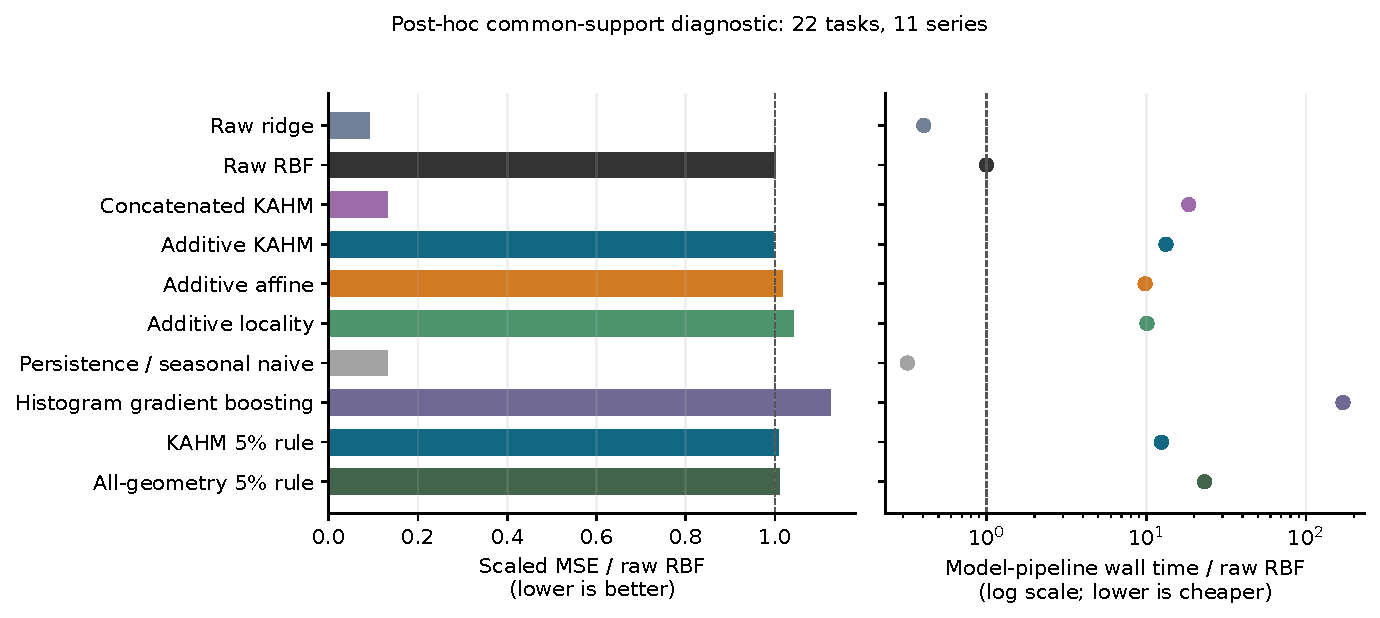
\includegraphics[width=\textwidth]{generated/utility/archive_accuracy_cost.pdf}
\caption{Post-hoc matched-success archive accuracy and cost relative to the raw RBF
procedure. Each ratio uses the equal-source aggregate; individual-source
heterogeneity is retained in Table~\ref{tab:utility-archive-sources}.
The time axis is logarithmic. No confidence interval across windows or
application-wide optimality claim is attached to these four-source
descriptive comparisons.}
\label{fig:utility-accuracy-cost}
\end{figure}
\FloatBarrier

\subsection{Realized residual alignment}
\label{app:utility-residual-results}

For each saved additive forecast, let
$d=\widehat f_{\rm add}(X)-\widehat f_{\rm raw}(X)$, which incorporates
the chosen mixing weight. The prespecified descriptive analysis
reconstructs $2\,\mathrm{mean}\langle Y-\widehat f_{\rm raw}(X),d\rangle$
and $\mathrm{mean}\|d\|^2$ directly from test predictions, averaging
target coordinates and dividing by the fixed training scale for each
archive task in the common-support diagnostic. Their difference equals the realized raw-minus-additive
MSE before rounding. The analysis code and independent manuscript
builder both verify this equality. Table~\ref{tab:utility-residual}
reports the same source hierarchy used for the main loss comparison.

This decomposition describes how the realized correction aligned with
the test residual, including its amplitude cost. It does not identify the
oracle conditional mean in Equation~\eqref{eq:utility-oracle}, explain
which representation component caused the alignment, or supply a new
out-of-sample guarantee. Test-derived terms are never used to retune
the correction, its mixing coefficient, or either adoption policy.

% Generated from the audited forecasting-utility extension; no model fitting.
\begin{table}[!htbp]
\centering\small\setlength{\tabcolsep}{4pt}
\caption{Descriptive test residual decomposition on the post-hoc common-support archive subset. For $d=\widehat f_{\rm add}-\widehat f_{\rm raw}$, alignment is $2\,\mathrm{mean}\langle Y-\widehat f_{\rm raw},d\rangle$ and energy is $\mathrm{mean}\|d\|^2$, averaged over target coordinates and divided by the fixed training scale before hierarchical aggregation. Raw-minus-additive MSE equals alignment minus energy before rounding. These are identities of the saved predictions, not fresh inference or a population certificate.}
\label{tab:utility-residual}
\begin{tabular}{llrrr}
\toprule
Source & Correction & Alignment & Energy & Gain \\
\midrule
Weather & Additive KAHM & -0.0024712 & 0.00068791 & -0.0031591 \\
Weather & Additive affine & 0.00021308 & 0.00097397 & -0.00076088 \\
Weather & Additive locality & -0.0004239 & 0.00036141 & -0.00078531 \\
Solar Weekly & Additive KAHM & 0 & 0 & 0 \\
Solar Weekly & Additive affine & 0 & 0 & 0 \\
Solar Weekly & Additive locality & 0.10669 & 0.059975 & 0.04671 \\
COVID-19 Deaths & Additive KAHM & 0.1667 & 0.045967 & 0.12074 \\
COVID-19 Deaths & Additive affine & -0.59915 & 0.029908 & -0.62906 \\
COVID-19 Deaths & Additive locality & -1.1003 & 0.15312 & -1.2534 \\
Car Parts & Additive KAHM & -0.00065859 & 0.0020919 & -0.0027505 \\
Car Parts & Additive affine & -0.00064528 & 0.0021013 & -0.0027466 \\
Car Parts & Additive locality & -0.058009 & 0.29197 & -0.34998 \\
\midrule
Equal-source mean & Additive KAHM & 0.040893 & 0.012187 & 0.028707 \\
Equal-source mean & Additive affine & -0.1499 & 0.0082457 & -0.15814 \\
Equal-source mean & Additive locality & -0.26301 & 0.12636 & -0.38936 \\
\bottomrule
\end{tabular}
\end{table}


\FloatBarrier
\section{Target-adapted geometry: theory, protocol, and complete results}
\label{app:target-geometry}

\subsection{Residual-target transport between fitted baselines}
\label{app:target-transport}

The following projection identity distinguishes residuals of a donor
baseline from residuals of the final baseline. Condition on the fitted
state, including a measurable representation
$\Gamma:\R^d\to\R^p$ and two predictors
$f_0,f_d:\R^d\to\R^H$. Let $(X,Y)$ be a fresh evaluation pair,
write $Z=\Gamma(X)$, and assume that $Y$, $f_0(X)$, and $f_d(X)$
have finite second moments. All expectations below refer to this
conditional evaluation distribution. For a fixed symmetric
positive-definite matrix $W\in\R^{H\times H}$, define
\[
 \langle a,b\rangle_W=a^\top Wb,\qquad
 \|a\|_W^2=a^\top Wa,\qquad
 R_W(f)=\E\|Y-f(X)\|_W^2.
\]
Here $a,b\in\R^H$. The equal-coordinate mean squared loss uses
$W=I_H/H$, where $I_H$ is the $H$-dimensional identity matrix.

\begin{proposition}[Correction gain and donor mismatch]
\label{prop:target-transport}
Define the conditional residual and conditional donor discrepancy by
\[
 m_0(Z)=\E[Y-f_0(X)\mid Z],\qquad
 b_d(Z)=\E[f_0(X)-f_d(X)\mid Z].
\]
For every measurable correction $q:\R^p\to\R^H$ satisfying
$\E\|q(Z)\|_2^2<\infty$,
\begin{equation}
 R_W(f_0)-R_W(f_0+q\circ\Gamma)
 =\E\|m_0(Z)\|_W^2-\E\|q(Z)-m_0(Z)\|_W^2.
 \label{eq:target-general-gain}
\end{equation}
The donor's optimal population correction is
$q_d(Z)=\E[Y-f_d(X)\mid Z]=m_0(Z)+b_d(Z)$. Hence
\begin{align}
 R_W(f_0)-R_W(f_0+q_d\circ\Gamma)
 &=\E\|m_0(Z)\|_W^2-\E\|b_d(Z)\|_W^2,
 \label{eq:target-transport-proof}\\
 R_W(f_0)-R_W(f_0+\widehat q\circ\Gamma)
 &=\E\|m_0(Z)\|_W^2-\E\|b_d(Z)+a(Z)\|_W^2,
 \label{eq:target-fitted-transport}
\end{align}
where $\widehat q$ is any square-integrable fitted correction and
$a(Z)=\widehat q(Z)-q_d(Z)$. Moreover,
\[
 \E\|b_d(Z)\|_W^2\leq\E\|f_0(X)-f_d(X)\|_W^2.
\]
\end{proposition}

\begin{proof}
Set $\epsilon=Y-f_0(X)-m_0(Z)$. By the definition of conditional
expectation, $\E[\epsilon\mid Z]=0$. Because $m_0(Z)-q(Z)$ is
measurable with respect to $Z$ and $W$ is fixed,
\[
 \E\langle\epsilon,m_0(Z)-q(Z)\rangle_W
 =\E\langle\E[\epsilon\mid Z],m_0(Z)-q(Z)\rangle_W=0.
\]
Expanding the squared norm of
$Y-f_0(X)-q(Z)=\epsilon+m_0(Z)-q(Z)$ therefore gives
\[
 R_W(f_0+q\circ\Gamma)
 =\E\|\epsilon\|_W^2+\E\|m_0(Z)-q(Z)\|_W^2.
\]
Set $q=0$ in this equality and subtract the general expression to
obtain Equation~\eqref{eq:target-general-gain}. Linearity of conditional
expectation gives
$q_d(Z)=m_0(Z)+b_d(Z)$. Substituting this correction proves
Equation~\eqref{eq:target-transport-proof}; substituting
$\widehat q(Z)=q_d(Z)+a(Z)$ proves
Equation~\eqref{eq:target-fitted-transport}.
Finally, the function $v\mapsto v^\top Wv$ is convex. Conditional
Jensen's inequality yields
\[
 \|\E[f_0(X)-f_d(X)\mid Z]\|_W^2
 \leq\E[\|f_0(X)-f_d(X)\|_W^2\mid Z].
\]
Taking expectations proves the bound on donor discrepancy.
\end{proof}

The final term in Equation~\eqref{eq:target-fitted-transport} contains
$2\E\langle b_d,a\rangle_W$. It cannot be replaced by separate
nonnegative mismatch and estimation penalties without another
orthogonality argument: approximation error may reinforce or partially
cancel the donor discrepancy. Even an exact donor correction can harm
the final base when its conditional mismatch exceeds the final base's
predictable residual signal.

For fixed square-integrable donors $f_1,\ldots,f_K$ and deterministic weights
$\pi_k\geq0$ summing to one, let $\bar f=\sum_k\pi_k f_k$.
Expanding around $\bar f$ gives
\[
 \sum_k\pi_k\E\|Y-f_k(X)-q(Z)\|_W^2
 =\E\|Y-\bar f(X)-q(Z)\|_W^2
  +\sum_k\pi_k\E\|f_k(X)-\bar f(X)\|_W^2.
\]
The cross term vanishes because the weighted donor deviations sum to
zero. Hence the common-law population optimizer is
$\E[Y-\bar f(X)\mid Z]$, and the proposition applies with
$f_d=\bar f$. This does not identify a finite OOF fit with that
optimizer. Chronological folds can have different laws and sample
sizes; a donor index depending on the observation must retain that
joint law rather than being replaced by constant mixture weights.

For a fixed realized correction $\delta(X)$ satisfying
$\E\|\delta(X)\|_2^2<\infty$, direct expansion also gives
\begin{equation}
 R_W(f_0)-R_W(f_0+\delta)
 =2\E\langle Y-f_0(X),\delta(X)\rangle_W
  -\E\|\delta(X)\|_W^2.
 \label{eq:target-alignment-audit}
\end{equation}
A separately implemented verification program checks its empirical
counterpart from saved test predictions. It does not estimate the oracle $m_0$ or $b_d$.
Donor/final disagreement is recorded separately on correction-training
rows. The final baseline has seen those rows, so this diagnostic is not
an unbiased estimate of future disagreement or predictive risk.

\subsection{Evaluation protocol and source roster}
\label{app:target-protocol}

The executable protocol is \path{extensions/target_geometry/PROTOCOL.md};
its configuration, numerical dependencies, implementation, and prepared
input roster were hashed before the full evaluation. Development checks use separate
seeds and do not enter confirmation. The synthetic seeds are
11200--11211. For law index $l$ and split index $s=0,1,2$, the generator in Appendix~\ref{c:app:methods} receives the first state value from
\texttt{SeedSequence([seed,l,s,9027])}. Each task has 128/64/128
training/validation/test episodes of length 72, history 12, offsets
$1,4,12$ and stride four, yielding 13 origins per episode.
Observation generation follows the same law-specific conventions as
the controlled study.

For synthetic OOF targets, episode index modulo four assigns folds.
Each donor excludes every row of the queried episodes. Within its
remaining episodes, the first 80\% of ordered episode IDs fit its
inner candidate models and the rest select its penalty. The selected
donor is then fitted on all donor episodes. No queried episode or
outer-validation target selects that donor's penalty.

For natural series, the first $\lceil0.4n\rceil$ capped training origins
initialize the donor history; the remainder form three contiguous query
blocks. If $t_b$ is the first query origin, only donor rows with
$t+H\leq t_b$ are allowed. An 80/20 inner chronological split applies
the same target-availability condition before inner validation.
Fewer than eight inner-fitting rows invokes the predefined donor
penalty one. Fewer than eight outer donor rows makes that query block
ineligible for \emph{both} residual-target procedures. The fitting
sample is otherwise fixed by indices, not by residual values or model
success. Fewer than eight eligible correction rows retains the available
baselines and sends the correction arms to their declared ridge fallback.
An eligible donor fit failure sends its dependent methods to that
fallback. An unavailable primary base or required evaluation split is
retained as a task failure.

\begin{table}[!htbp]
\centering\small\setlength{\tabcolsep}{4pt}
\caption{Archive collections and fixed target-geometry roster.
$L$ is history length, $H$ the number of consecutive target steps, and
$p$ the seasonal period. Selection uses only training-prefix eligibility
and identifier hashes. These are 12 series from four selected collections,
not 12 independent application domains.}
\label{tab:target-roster}
\begin{tabular}{llrrrl}
\toprule
Collection & Frequency & $L$ & $H$ & $p$ & Selected series \\
\midrule
Australian electricity & Half-hourly & 48 & 12 & 48 & T3, T5, T1 \\
Bitcoin indicators & Daily & 28 & 7 & 7 & \begin{tabular}[t]{@{}l@{}}sent\_addresses, confirmation\_time,\\block\_size\end{tabular} \\
Melbourne pedestrian & Hourly & 48 & 6 & 24 & T10, T14, T20 \\
KDD2018 air quality & Hourly & 48 & 6 & 24 & T239, T99, T233 \\
\bottomrule
\end{tabular}
\end{table}

The source records are respectively
\href{https://doi.org/10.5281/zenodo.4659727}{10.5281/zenodo.4659727},
\href{https://doi.org/10.5281/zenodo.5121965}{10.5281/zenodo.5121965},
\href{https://doi.org/10.5281/zenodo.4656626}{10.5281/zenodo.4656626}, and
\href{https://doi.org/10.5281/zenodo.4656719}{10.5281/zenodo.4656719}.
All selected archive versions declare CC BY 4.0; archive/member hashes, attribution,
source exclusions and metadata are retained in
\path{extensions/target_geometry/sources/manifest.json}.
Bitcoin selections are activity indicators, not price forecasts.
These collections broaden source coverage but are not sampled randomly
from application domains. The study uses fixed archive versions and
does not reconstruct historical data-release vintages.

Training-prefix eligibility requires 96 finite windows and a positive
seasonal-difference mean-square scale, with first-difference fallback.
The selection salt is
\texttt{kahm-target-geometry-new-collections-v1}. Each series uses
chronological 60/20/20 splits. Training is capped at 512 windows and
validation/test at 64 origins per segment by even index spacing.
All targets lie inside their segment; later test histories can contain
already observed test values. Missing windows are excluded without
interpolation, defining an available-window estimand. The loss scale
uses the initial training prefix only. The naive control uses the
declared seasonal lag with an available-value fallback; synthetic
naive prediction is persistence.

The 18 primary contrasts use 12 paired repetition-level means each.
For positive differences favoring the second method, they compare
ridge with learned-OOF KAHM; identity-OOF KAHM with learned-OOF KAHM;
identity-in-sample KAHM with identity-OOF KAHM; and learned-OOF affine,
locality, and RBF-local with learned-OOF KAHM. For paired differences $d_1,\ldots,d_{12}$, let $\bar d$ be their
mean and $s_d$ their sample standard deviation. The interval is
$\bar d\pm t_{11,1-0.05/(2\cdot18)}s_d/\sqrt{12}$, where
$t_{\nu,p}$ is the $p$ quantile of Student's $t$ distribution with
$\nu$ degrees of freedom. Simultaneous coverage uses the stated
normal approximation. No joint coverage is asserted with prior study
families. Archive results and leave-one-source-out re-aggregations are
descriptive; no window-based confidence interval is attached to four
selected source collections.

\subsection{Implementation, safeguards, and accounting}
\label{app:target-implementation}

The metric uniformly samples up to 256 correction rows without
replacement using the task seed. All training inputs determine its
input standardizer, matching the downstream bank; only eligible OOF
residual targets fit its supervised objective. Its donor mask excludes
whole synthetic episodes or natural origins separated by at most
$L+H$. Queries with no admissible donor are omitted from the proxy;
fewer than two admissible queries or donor groups invokes identity.
For $n_c$ eligible residual rows $r_i\in\R^H$, define
$\bar r_h=n_c^{-1}\sum_{i=1}^{n_c}r_{ih}$. The pooled residual scale is
$[ (n_cH)^{-1}\sum_{i=1}^{n_c}\sum_{h=1}^{H}(r_{ih}-\bar r_h)^2]^{1/2}$,
computed before row subsampling.
Constant residuals or absence of positive admissible input distances
also invoke identity. Log-sum-exp evaluates kernel probabilities.
L-BFGS-B uses \texttt{ftol=$10^{-10}$},
\texttt{gtol=$10^{-6}$}, at most 40 iterations and 20 line-search
steps. The source retains the analytic derivative, numerical gradient
check, fitted weights, objective values, donor counts, optimizer status
and fallback reason. Training-objective improvement is not a forecast
accuracy claim.

Each bank caps every requested group count by the number of distinct
sampled partition histories. If numerical clustering still has empty
groups, all counts are halved down to one, with each reduction recorded.
Rank-zero local models return their reference center.
Unexpected geometry or correction errors return the fitted ridge
forecast with the exception and incurred work retained. A failed
supervised metric uses identity; a failed secondary raw RBF also uses
ridge. A numerical failure of the secondary jointly fitted head is
isolated to that arm and invokes the same ridge fallback. These fallback rules are specified for this experiment; the additive
study in Section~\ref{sec:utility-extension} used a different failure policy.

KAHM, affine and locality codes import the archived reconstruction and
coordinate formulas. The RBF-local gate for local model $c$ uses
$\exp\{-\|z-\mu_c\|_2^2/(2s_c)\}$, normalized within its block,
where $s_c$ is its reference mean squared radius, floored at $10^{-6}$.
All four multiply local coordinates by their corresponding affinities.
Applying metric weights before re-standardizing each input column
would cancel the intended metric; the implementation instead applies
$\operatorname{diag}(e^{\theta/2})$ after the shared standardizer.
Identity-weight tests recover archived features on nondegenerate data.

One task and one numerical-library thread execute at a time. Disjoint
wall and process-CPU nodes record base search/prediction, donor fitting,
metric learning, bank construction and transformations, head search,
final prediction and selected-model serialization. Each procedure pays
for its required nodes once, including a rejected correction's search.
Test feature transformations are conservatively charged even when
zero correction bypasses their subsequent use; they consume test
inputs only. Imports, data download/preparation, artifact writes and
reporting are outside model timing. Serialized bytes describe the
retained model state, not an information-theoretic storage minimum.

\subsection{Complete comparisons and diagnostic records}
\label{app:target-results}

The tables and figures report all primary contrasts and every source. The separately implemented
analyzer recomputes losses from saved targets and predictions, checks
the complete task/method roster, validates donor exclusions and
selection records, sums charged dependencies, checks zero-correction
equality, and verifies Equation~\eqref{eq:target-alignment-audit}.
Metric objectives, effective groups, selected mixing weights and
donor/final disagreement remain diagnostics of the declared procedures.
Neither these quantities nor a smaller proxy objective estimates
unrestricted Bayes risk, identifies minimum necessary complexity, or
certifies a universal KAHM adoption rule.

\paragraph{Primary contrasts and source sensitivity.}
Figure~\ref{fig:target-synthetic-contrasts} displays the complete
18-contrast family, with numerical endpoints in
Table~\ref{tab:target-synthetic-intervals}. The three ridge contrasts
favor learned-OOF KAHM, while five matched-geometry contrasts favor
the simpler control. None establishes a learned-metric or OOF-target
increment for KAHM. Table~\ref{tab:target-archive-sources} retains
the source means, and Table~\ref{tab:target-archive-windows} records
every series's windows and training loss scale. Individual-series
losses are retained in \path{reports/task_metrics.csv} in the target-geometry reproduction directory. Learned-OOF KAHM's source-mean
reductions relative to ridge are 3.91\% for Australian electricity,
1.38\% for Bitcoin indicators, 4.37\% for pedestrian counts, and
0.85\% for air quality. The favorable source means coexist with higher loss on four
individual series. The complete leave-one-source-out
display in Table~\ref{tab:target-leave-one-source-out} concerns
composition sensitivity of this roster, not uncertainty over new
collections.

\paragraph{Optimization and residual diagnostics.}
All 36 synthetic and 12 archive metric fits report optimizer
convergence; none invokes identity fallback or reaches the iteration
limit. There are no recorded bank group reductions or fitting warnings.
Synthetic optimization takes two to three iterations and decreases
the regularized objective by a median $1.8741\times10^{-6}$; the
learned maximum-to-minimum weight ratios span 1.0013--1.1054. The
synthetic metric therefore remains close to identity under the frozen
bandwidth, penalty and diagonal parameterization. Archive optimization
takes two to 14 iterations, with median objective decrease
$2.9692\times10^{-4}$ and weight ratios 1.0577--16.0000. One pedestrian
series reaches the declared ratio cap. These are observed solver
statuses and training-objective changes, not guarantees of global
optimality, forecasting improvement, or performance of an
end-to-end KAHM metric.

The median correction-row donor/final disagreement divided by OOF
residual MSE is 0.0024 for synthetic tasks and 0.1047 for archive tasks
(Table~\ref{tab:target-diagnostics}). This descriptive difference
documents that the two residual sources need not be interchangeable;
it cannot identify the oracle transport penalty in
Proposition~\ref{prop:target-transport} or attribute observed test
differences to that penalty. Validation selects full-strength
learned-OOF KAHM correction on 35 of 36 synthetic tasks, with half
strength on the remaining task. Archive selections are more restrained:
the counts for $\gamma=0,1/4,1/2,1$ are $1,4,6,1$
(Table~\ref{tab:target-selection}). The four archive series harmed
despite nonzero validation selection confirm that the available zero
option does not ensure improvement on future observations.

\begin{figure}[!htbp]
\centering
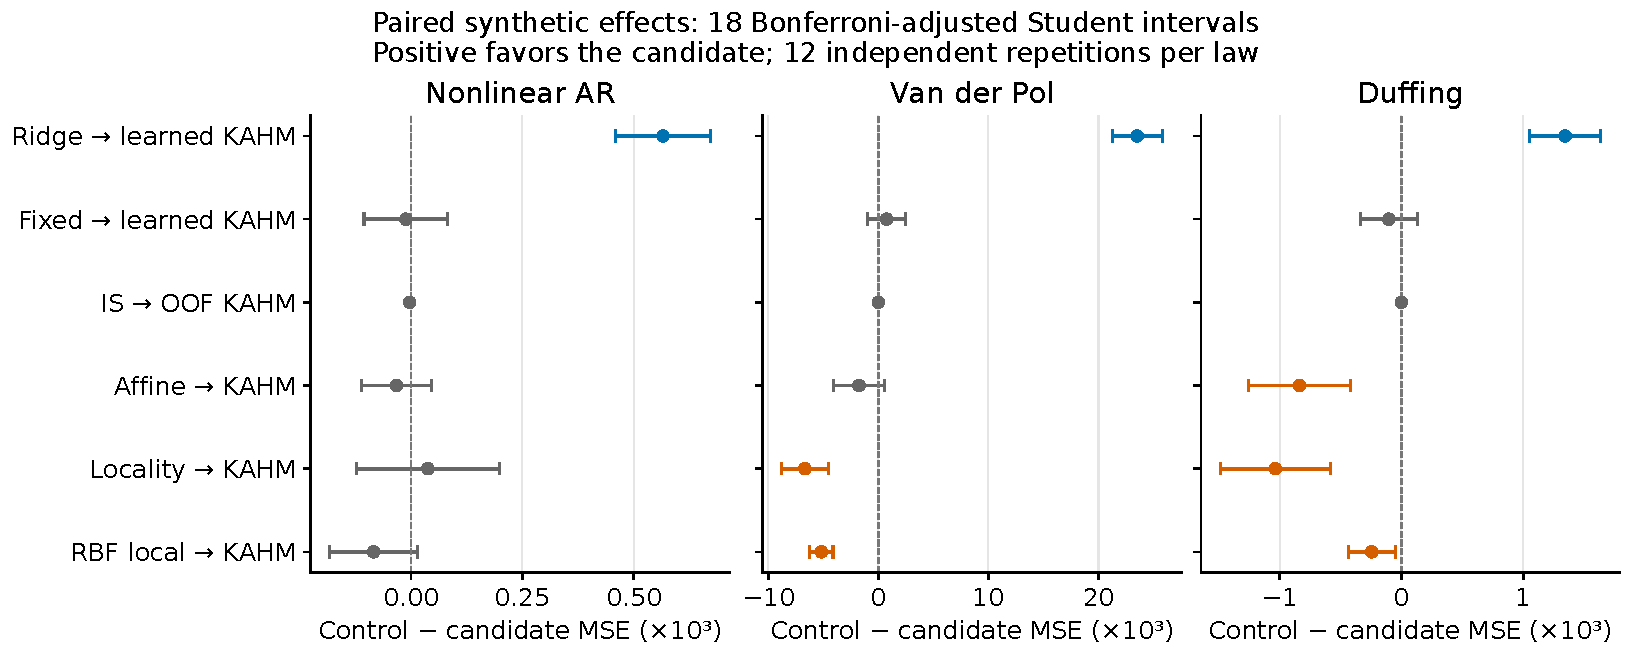
\includegraphics[width=\linewidth]{generated/target_geometry/synthetic_contrasts.pdf}
\caption{All six prescribed contrasts for each known synthetic law.
Points are paired mean differences in MSE, multiplied by $10^3$;
positive values favor the candidate named to the right of each arrow.
Intervals use the common 18-comparison Bonferroni adjustment and
12 independent repetition differences per law. The learned-metric
comparison holds OOF targets fixed; the residual-target comparison
holds the identity metric fixed. Matched-geometry comparisons use
the shared learned metric and OOF targets. Each panel has its own
horizontal range, and intervals containing zero are unresolved,
not evidence of equal performance.}
\label{fig:target-synthetic-contrasts}
\end{figure}

% Generated only from audited target-geometry predictions; no fitting.
\begin{table}[!htbp]
\centering\scriptsize\setlength{\tabcolsep}{4pt}
\caption{The complete family of 18 prespecified synthetic comparisons. $\Delta$ is control minus candidate test MSE; positive values favor the candidate. Intervals use the paired repetition differences, Student's $t_{11}$ quantile, and a two-sided Bonferroni allocation of $0.05/18$. Family coverage is approximate because normality of repetition differences is not guaranteed. No claim joins this family to earlier experiments.}
\label{tab:target-synthetic-intervals}
\begin{tabular}{lllrr}
\toprule
Law & Control & Candidate & $\Delta\times10^3$ & Family interval \\
\midrule
Nonlinear AR & Raw ridge & Learned, OOF KAHM & 0.566 & [0.459, 0.672] \\
Nonlinear AR & Fixed, OOF KAHM & Learned, OOF KAHM & -0.011 & [-0.105, 0.083] \\
Nonlinear AR & Fixed, IS KAHM & Fixed, OOF KAHM & -0.003 & [-0.006, $4.07\times10^{-4}$] \\
Nonlinear AR & Learned, OOF Affine & Learned, OOF KAHM & -0.032 & [-0.111, 0.046] \\
Nonlinear AR & Learned, OOF Locality & Learned, OOF KAHM & 0.038 & [-0.122, 0.199] \\
Nonlinear AR & Learned, OOF RBF local & Learned, OOF KAHM & -0.083 & [-0.182, 0.015] \\
Van der Pol & Raw ridge & Learned, OOF KAHM & 23.510 & [21.236, 25.785] \\
Van der Pol & Fixed, OOF KAHM & Learned, OOF KAHM & 0.754 & [-0.939, 2.447] \\
Van der Pol & Fixed, IS KAHM & Fixed, OOF KAHM & -0.003 & [-0.008, 0.002] \\
Van der Pol & Learned, OOF Affine & Learned, OOF KAHM & -1.751 & [-4.088, 0.586] \\
Van der Pol & Learned, OOF Locality & Learned, OOF KAHM & -6.661 & [-8.765, -4.558] \\
Van der Pol & Learned, OOF RBF local & Learned, OOF KAHM & -5.169 & [-6.229, -4.110] \\
Duffing & Raw ridge & Learned, OOF KAHM & 1.344 & [1.054, 1.634] \\
Duffing & Fixed, OOF KAHM & Learned, OOF KAHM & -0.103 & [-0.336, 0.130] \\
Duffing & Fixed, IS KAHM & Fixed, OOF KAHM & -0.001 & [-0.006, 0.004] \\
Duffing & Learned, OOF Affine & Learned, OOF KAHM & -0.836 & [-1.254, -0.418] \\
Duffing & Learned, OOF Locality & Learned, OOF KAHM & -1.036 & [-1.489, -0.583] \\
Duffing & Learned, OOF RBF local & Learned, OOF KAHM & -0.243 & [-0.435, -0.051] \\
\bottomrule
\end{tabular}
\end{table}

% Generated only from audited target-geometry predictions; no fitting.
\begin{table}[!htbp]
\centering\small\setlength{\tabcolsep}{4pt}
\caption{Scaled MSE by collection, averaging its three declared series. Collections receive equal weights in the aggregate; neither series nor repeated origins increase the collection count. No confidence intervals are attached to these four descriptive collection means.}
\label{tab:target-archive-sources}
\begin{tabular}{lrrrr}
\toprule
Procedure & Electricity & Bitcoin & Pedestrian & Air quality \\
\midrule
Raw ridge & 0.2879 & 3.0946 & 1.2489 & 0.5704 \\
Raw RBF & 0.2969 & 5.8096 & 1.0650 & 0.6216 \\
Persistence / seasonal naive & 0.7859 & 3.3622 & 1.5349 & 1.7073 \\
Joint raw + KAHM & 0.2760 & 3.8872 & 1.0713 & 0.5773 \\
Fixed, IS KAHM & 0.2725 & 3.0163 & 1.1943 & 0.5752 \\
Fixed, IS Affine & 0.2753 & 3.0013 & 1.1862 & 0.5708 \\
Fixed, IS Locality & 0.2678 & 3.0174 & 1.1882 & 0.5808 \\
Fixed, IS RBF local & 0.2885 & 3.0102 & 1.1697 & 0.5631 \\
Fixed, OOF KAHM & 0.2778 & 3.0781 & 1.1766 & 0.5741 \\
Fixed, OOF Affine & 0.2798 & 3.0762 & 1.1636 & 0.5728 \\
Fixed, OOF Locality & 0.2713 & 3.0559 & 1.1781 & 0.5887 \\
Fixed, OOF RBF local & 0.2828 & 3.0424 & 1.2035 & 0.5695 \\
Learned, OOF KAHM & 0.2766 & 3.0520 & 1.1943 & 0.5656 \\
Learned, OOF Affine & 0.2975 & 3.0369 & 1.1691 & 0.5711 \\
Learned, OOF Locality & 0.2751 & 3.0615 & 1.1597 & 0.5714 \\
Learned, OOF RBF local & 0.2838 & 3.0506 & 1.2278 & 0.5772 \\
\bottomrule
\end{tabular}
\end{table}

% Generated only from audited target-geometry predictions; no fitting.
\begin{table}[!htbp]
\centering\scriptsize\setlength{\tabcolsep}{4pt}
\caption{Exact natural-series roster, selected before forecasts by a salted hash among training-prefix-eligible candidates. $L$ is history length and $H$ the complete forecast path length. Chronological boundaries are 60/20/20; windows with missing inputs or targets are omitted without imputation. At most 512/64/64 windows are retained by the frozen deterministic sampling rule. The loss scale is computed before validation. Bitcoin series are network indicators, not prices.}
\label{tab:target-archive-windows}
\begin{tabular}{llrrrr}
\toprule
Collection & Series & $L$ & $H$ & Train/val/test & Loss scale \\
\midrule
Australian electricity & T3 & 48 & 12 & 512/64/64 & $1.43\times10^{5}$ \\
Australian electricity & T5 & 48 & 12 & 512/64/64 & 4182.897 \\
Australian electricity & T1 & 48 & 12 & 512/64/64 & $4.50\times10^{5}$ \\
Bitcoin indicators & sent\_addresses & 28 & 7 & 512/64/64 & $2.07\times10^{8}$ \\
Bitcoin indicators & confirmation\_time & 28 & 7 & 512/64/64 & 163.705 \\
Bitcoin indicators & block\_size & 28 & 7 & 512/64/64 & $3.19\times10^{9}$ \\
Pedestrian counts & T10 & 48 & 6 & 512/64/64 & 26088.371 \\
Pedestrian counts & T14 & 48 & 6 & 512/64/64 & 31655.986 \\
Pedestrian counts & T20 & 48 & 6 & 512/64/64 & 27784.521 \\
KDD air quality & T239 & 48 & 6 & 512/64/64 & 102.986 \\
KDD air quality & T99 & 48 & 6 & 512/64/64 & 226.458 \\
KDD air quality & T233 & 48 & 6 & 512/64/64 & 441.826 \\
\bottomrule
\end{tabular}
\end{table}

% Generated only from audited target-geometry predictions; no fitting.
\begin{table}[!htbp]
\centering\scriptsize\setlength{\tabcolsep}{4pt}
\caption{Training diagnostics, not independent evidence of test benefit. $\mathcal J$ is the regularized Gaussian residual-regression proxy shared by all geometric arms. $\mathcal J_0$ and $\mathcal J_{\rm fit}$ are the identity-metric and selected fitted-metric objectives. A finite improved iterate may be retained at an iteration limit, separately from optimizer convergence. $D$ is mean squared disagreement between donor and final ridge predictions on the same correction rows; $R_{\rm OOF}$ is their out-of-fold (OOF) residual MSE. Medians summarize observed tasks and are descriptive. Exact objectives, warnings, weight ratios, missing diagnostics and residual identities are retained in the report CSV files.}
\label{tab:target-diagnostics}
\begin{tabular}{lrrrrr}
\toprule
Phase & Tasks & Converged & Metric fallback & Median $\mathcal J_0-\mathcal J_{\rm fit}$ & Median $D/R_{\rm OOF}$ \\
\midrule
Synthetic & 36 & 36 & 0 & $1.874\times10^{-6}$ & 0.0024 \\
Archive & 12 & 12 & 0 & 0.0003 & 0.1047 \\
\bottomrule
\end{tabular}
\end{table}

% Generated only from audited target-geometry predictions; no fitting.
\begin{table}[!htbp]
\centering\scriptsize\setlength{\tabcolsep}{4pt}
\caption{Validation-selected correction strengths, with counts ordered as $\gamma=0,0.25,0.5,1$. A zero correction is the exact deployed ridge predictor. A failed arm is recorded separately as a baseline fallback, not as an observed zero-strength validation selection. Selection counts summarize tasks and do not supply an additional inference sample.}
\label{tab:target-selection}
\begin{tabular}{lrrrr}
\toprule
Procedure & Synthetic gamma counts & Fallback & Archive gamma counts & Fallback \\
\midrule
Fixed, IS KAHM & 0 / 0 / 0 / 36 & 0 & 1 / 5 / 1 / 5 & 0 \\
Fixed, IS Affine & 0 / 0 / 1 / 35 & 0 & 2 / 3 / 2 / 5 & 0 \\
Fixed, IS Locality & 0 / 0 / 1 / 35 & 0 & 0 / 3 / 5 / 4 & 0 \\
Fixed, IS RBF local & 0 / 0 / 0 / 36 & 0 & 0 / 3 / 5 / 4 & 0 \\
Fixed, OOF KAHM & 0 / 0 / 0 / 36 & 0 & 2 / 5 / 2 / 3 & 0 \\
Fixed, OOF Affine & 0 / 0 / 1 / 35 & 0 & 3 / 4 / 4 / 1 & 0 \\
Fixed, OOF Locality & 0 / 0 / 1 / 35 & 0 & 0 / 7 / 4 / 1 & 0 \\
Fixed, OOF RBF local & 0 / 0 / 0 / 36 & 0 & 1 / 4 / 6 / 1 & 0 \\
Learned, OOF KAHM & 0 / 0 / 1 / 35 & 0 & 1 / 4 / 6 / 1 & 0 \\
Learned, OOF Affine & 0 / 0 / 1 / 35 & 0 & 1 / 4 / 5 / 2 & 0 \\
Learned, OOF Locality & 0 / 0 / 1 / 35 & 0 & 1 / 4 / 7 / 0 & 0 \\
Learned, OOF RBF local & 0 / 0 / 0 / 36 & 0 & 0 / 5 / 5 / 2 & 0 \\
\bottomrule
\end{tabular}
\end{table}

% Generated only from audited target-geometry predictions; no fitting.
\begin{table}[!htbp]
\centering\small\setlength{\tabcolsep}{4pt}
\caption{Descriptive sensitivity to collection composition: each column omits the named collection and recomputes the mean scaled loss over the remaining three collections, divided by the corresponding raw-ridge loss. Values below one favor the procedure. Every omission is shown; none is selected as the primary result. These ratios are not independent replications, confidence intervals, or additional confirmatory tests.}
\label{tab:target-leave-one-source-out}
\begin{tabular}{lrrrr}
\toprule
Procedure & Electricity & Bitcoin & Pedestrian & Air quality \\
\midrule
Raw ridge & 1.000 & 1.000 & 1.000 & 1.000 \\
Raw RBF & 1.526 & 0.941 & 1.702 & 1.548 \\
Persistence / seasonal naive & 1.344 & 1.912 & 1.481 & 1.227 \\
Joint raw + KAHM & 1.127 & 0.913 & 1.199 & 1.130 \\
Fixed, IS KAHM & 0.974 & 0.969 & 0.977 & 0.968 \\
Fixed, IS Affine & 0.968 & 0.964 & 0.973 & 0.964 \\
Fixed, IS Locality & 0.974 & 0.967 & 0.978 & 0.966 \\
Fixed, IS RBF local & 0.965 & 0.959 & 0.977 & 0.965 \\
Fixed, OOF KAHM & 0.983 & 0.963 & 0.994 & 0.979 \\
Fixed, OOF Affine & 0.979 & 0.957 & 0.994 & 0.976 \\
Fixed, OOF Locality & 0.981 & 0.967 & 0.991 & 0.973 \\
Fixed, OOF RBF local & 0.980 & 0.976 & 0.985 & 0.978 \\
Learned, OOF KAHM & 0.979 & 0.966 & 0.985 & 0.977 \\
Learned, OOF Affine & 0.972 & 0.967 & 0.988 & 0.972 \\
Learned, OOF Locality & 0.975 & 0.952 & 0.989 & 0.971 \\
Learned, OOF RBF local & 0.988 & 0.991 & 0.990 & 0.985 \\
\bottomrule
\end{tabular}
\end{table}

\FloatBarrier

\FloatBarrier
\section{Direct reconstruction protocol and reproducibility}
\label{app:direct-protocol}

The protocol in \path{extensions/direct_reconstruction/PROTOCOL.md}
specifies the model, input preparation, optimization, analysis, and
exact task roster. Its public checkpoint includes the implementation,
numerical dependencies, source metadata, and prepared input arrays and
precedes evaluation on D. The exploratory gate-training pilot has a
separate design and does not contribute observations to the primary
interval family.

\paragraph{Local shape controls and gate normalization.}
Use the row-stored reference matrix, principal basis, and center from
Section~\ref{sec:direct-reconstruction}. Let $b(c)$ be the partition
block containing local model $c$, and set
\[
 a_c(z)=\mu_c+P_cP_c^\top(z-\mu_c),\quad
 u_c(z)=P_c^\top(z-\mu_c),\quad
 n_c(z)=(I_L-P_cP_c^\top)(z-\mu_c).
\]
The scalars $t_c$ and $e_c$ are the positive reference-radius and
projection-residual scales in Equation~\eqref{eq:nf-locality-gates}.
For a horizon-specific shape parameter $\xi_b$, the affine control uses
\[
 r_c^{\mathrm A}(z;\xi_b)=\mu_c+e^{\xi_b}P_cP_c^\top(z-\mu_c).
\]
Both this reconstruction and the KAHM reconstruction determine a folding
score $s_c$ through Equation~\eqref{eq:nf-folding-gates}. Their gate
logit is
$\ell_c(z)=16\log[1-\operatorname{clip}_{[0,1]}s_c(z)+10^{-6}]$.
The other two controls use logits
\begin{align*}
 \ell_c^{\mathrm{loc}}(z;\xi_b)
 &=-e^{\xi_b}\frac{\|n_c(z)\|_2^2}{e_c}
   -0.1e^{-\xi_b}\frac{\|z-\mu_c\|_2^2}{t_c},\\
 \ell_c^{\mathrm{RBF}}(z;\xi_b)
 &=-\frac{e^{\xi_b}\|u_c(z)\|_2^2+
                e^{-\xi_b}\|n_c(z)\|_2^2}{2t_c}.
\end{align*}
For every family, the temperature parameter $\eta_b$ gives the gate
\[
 \phi_c(z)=\frac{\exp\{e^{\eta_b}\ell_c(z)\}}
 {\sum_{j\in\mathcal C_b}\exp\{e^{\eta_b}\ell_j(z)\}},
 \qquad c\in\mathcal C_b.
\]
Both parameters lie in $[-\log4,\log4]$. The fixed model sets both to
zero, the gate-trained model fixes $\xi_b=0$, and the shape-trained
model fits both. The principal coordinates $u_c$ themselves remain
fixed in all three procedures.

The optimizer is L-BFGS-B with numerical forward differences, at most
40 iterations, at most 20 line-search steps per iteration, function
tolerance $10^{-10}$, and gradient tolerance $10^{-6}$. Its 256-evaluation
ceiling counts actual objective calls, including calls used for numerical
differentiation. A zero parameter vector initializes every optimization,
and the best finite evaluated parameter vector supplies the fitted state.

\paragraph{Exploratory gate-training pilot.}
The pilot used three independent seeds per law, separately implemented
generators, and at most 160 objective evaluations. Gate-temperature
training reduced mean KAHM MSE relative to its fixed version by 0.53\%
on nonlinear AR, 30.21\% on Van der Pol, and 11.29\% on Duffing. The
best directly trained local control was more accurate on every law;
raw RBF was also substantially stronger on Van der Pol and Duffing.
The reproduction materials contain all 99 method--task prediction
records and their optimization outcomes. These nine exploratory tasks
are excluded from the direct-reconstruction interval family.

\paragraph{Chronology and seasonal prediction.}
Synthetic seeds are 84200--84211 for each law, with
72-observation episodes and thirteen forecast origins per episode.
Implementation checks use seed 932001, outside the evaluation roster.
Whole-episode inner validation selects the raw baseline in A. For natural
data, inner A training targets must have matured by its first
validation query. Every outer target lies inside its segment. A history
can include observations from the preceding segment because these have
already been observed at the forecast origin. No future missing-value
imputation or label-based series replacement is used.

Dominick has history 52, offsets $(1,2,4)$ and seasonal period 52.
Rideshare uses only \texttt{price\_mean} series, history 24, offsets
$(1,3,6)$ and period 24. An A-only availability check reduced the
proposed history from 48 to 24 before the public checkpoint and any
forecast evaluation; the seasonal period and eligibility threshold
were unchanged. Wikipedia has history 28, offsets $(1,3,7)$ and
period 7. Sunspot uses the last 4,096 observations independent of their
values, history 28, offsets $(1,3,7)$ and period one. Each of the first
three collections contributes three hash-selected eligible series;
sunspot contributes its single series. Every source record, archive
checksum, selected identifier, original origin index, split boundary and
training-only scale is included in the reproduction records. Natural row caps are 512/128/128/128.
The minimum A eligibility is 96 complete windows with a positive finite
scale. A later unavailable segment remains a recorded failure. The three selected
rideshare series have no complete B windows, identified during preparation
after A-only selection; all three are retained as planned feasibility
failures. This precludes a complete four-collection accuracy aggregate.

Synthetic task MSE averages squared errors over the three offsets and
all D origins. Natural task MSE is divided by an A-only scale: the mean
of finite squared differences at the collection's seasonal period. If
this mean is unavailable, nonfinite, or nonpositive, the corresponding
first-difference mean is used. A task with no positive finite scale is
ineligible. The scale remains fixed throughout selection and evaluation.
All source-level means weight the selected series equally.

For a primary synthetic comparison, let $d_r$ be comparator MSE minus
reconstruction-trained KAHM MSE in repetition $r$, for $r=1,\ldots,12$.
With sample mean $\bar d$ and sample standard deviation $s_d$, the
95\% Bonferroni-adjusted interval is
\[
 \bar d\ \pm\ t_{11,1-0.05/(2\cdot18)}\frac{s_d}{\sqrt{12}},
\]
where $t_{\nu,q}$ denotes the $q$ quantile of Student's $t$ distribution
with $\nu$ degrees of freedom. Under independent normal paired
differences, these intervals jointly cover all eighteen population mean
differences with probability at least 95\%; otherwise the coverage
uses a normal approximation. The statistical unit is the complete
repetition, not an individual forecast origin.

Seasonal naive predicts each offset from the most recent observed value
with the appropriate seasonal phase. For period $p$ this is
$y_{t+h-p\lceil h/p\rceil}$, using only indices at or before $t$.
Period one therefore gives persistence. All declared histories include
the required seasonal lag. The selected source records are
\url{https://doi.org/10.5281/zenodo.4654802},
\url{https://doi.org/10.5281/zenodo.5122114},
\url{https://doi.org/10.5281/zenodo.4656080}, and
\url{https://doi.org/10.5281/zenodo.4654773}; the source manifest retains
attribution and archive-license metadata.

\paragraph{Baseline and correction selection.}
Raw RBF and boosting retain the fitted ridge state for a recorded
horizon-wise D fallback; a D failure cannot change their C forecast or
the C-selected policy. Its baseline cost and serialized bytes are included.
Raw ridge uses penalties $10^{-4},10^{-3},10^{-2},10^{-1},1,10,100$,
selected inside A and then refitted on A. The raw RBF reference retains
raw standardized history together with at most 64 Nystr\"om landmarks;
bandwidth factors $0.5,1,2$ multiply the median positive landmark
squared-distance scale, and B selects among them and the same seven
penalties.
Histogram gradient boosting fits 100 iterations with L2 penalty one,
learning rate $0.05$ or $0.1$, and maximum leaves 7 or 15; B selects the
grid jointly across horizons without external early stopping, using
a separate fitted tree ensemble per target. All local corrections use the
same A residual targets, sum-loss penalties $0.01,0.1,1$, A-standardized
features and unpenalized intercept. C chooses their mixing weights
separately by horizon with the zero-correction tie-breaking rule. A budget exit or
nonfinite trial is logged; the best finite incumbent is retained.

The affine gain and locality/RBF anisotropy are deliberately different
functional interventions from the KAHM bandwidth. Their common parameter
counts, supervision and evaluation ceilings support a matched experiment
at that level; they do not prove equal approximation power or equal
computation. Likewise, a gate-only arm has three parameters per horizon
and a reconstruction/shape arm has six, so their comparison asks whether
the additional intervention helps within the declared budget.

\paragraph{Computation and state.}
Numerical-library thread counts are fixed to one. Warm measured nodes
cover the baseline, shared bank, KAHM-specific factors, all paid geometry
trials, C selection, and D transformations and predictions. The implementation eagerly prepares
fixed gate queries and charges that work even when C selects zero
correction or a different bandwidth; the accounting is conservative
relative to a possible lazy implementation.
Each standalone procedure sums its required dependencies once. Policy
costs sum the union of measured candidate dependencies, including their
eager query work, not only the selected winner. This component sum is not
a separately timed minimal policy execution. Selected fitted states, their serialized byte sizes and
serialization time are retained. Downloads, input preparation, imports
and evidence artifact writing lie outside the model pipeline. Absolute
times and ratios describe this implementation and host, not intrinsic
algorithmic constants. A whole-process high-water RSS is not a
per-method memory estimate.

The evaluation compares fixed computational search budgets rather than
equal measured wall times. It does not evaluate delayed-label updates
or drifting streams; those questions are addressed separately in
Section~\ref{sec:adaptive-development}.

\paragraph{Computational verification.}
The verification program checks archived inputs and source files, reconstructs
windows from retained raw episodes or series, recomputes C/D losses,
checks all method and candidate rosters, replays strict selection,
checks exact zero correction, reconstructs cost dependencies and
replays serialized selected predictions. The program passes 543,017 consistency checks, including reconstruction
of 144 generated episode batches and replay of 731 selected states on
C and D. A separate calculation recomputes scalar losses, A-only
natural scales, and all 18 intervals without importing the model or
its analyzer. Neither check independently refits every optimization
trial or supplies an external experimental replication.

Bitwise regeneration also depends on the numerical environment. The
recorded execution uses NumPy 2.3.5 on an AVX512-capable x86-64 host.
A post-execution diagnostic reproduces all four episode batches of one
declared Duffing task exactly on that host, but disabling AVX512 dispatch
changes some values at floating-point roundoff scale. Package versions
and single-thread execution alone therefore do not guarantee identical
regenerated bytes on other processors. The archived input arrays therefore provide the exact evaluated inputs.
Regeneration checks compare their bytes exactly, whereas selected-state
prediction replay uses an absolute and relative tolerance of $10^{-10}$.
A separate raw-RBF state probe crosses the declared $10^{-10}$ absolute
and relative replay tolerances under altered dispatch, while changing
its C/D mean squared errors by less than $10^{-14}$ relatively.
Verification succeeds on the original host and on one compatible hosted
environment. The altered-dispatch failures identify a limitation of
strict numerical replay across processor configurations.


\subsection{Complete comparisons and resource records}

\begin{table}[!htbp]
\centering\small
\setlength{\tabcolsep}{4pt}
\caption{The complete 18-comparison family for reconstruction-trained
KAHM. With $\overline L$ denoting mean MSE across twelve repetitions,
gain is $100(\overline L_{\rm control}-\overline L_{\rm KAHM})/
\overline L_{\rm control}$. Intervals are absolute paired MSE differences,
not percentage intervals; their positive direction favors KAHM.}
\label{tab:direct-primary}
\begin{tabular}{llrrl}
\toprule
Law & Control & Gain (\%) & Difference interval & Outcome \\
\midrule
AR & Raw RBF & 2.87 & [6.65e-06, 0.000278] & positive \\
AR & Gate KAHM & 0.09 & [-3.86e-05, 4.71e-05] & unresolved \\
AR & Reconstruction affine & -0.11 & [-0.0001, 8.97e-05] & unresolved \\
AR & Reconstruction locality & 1.11 & [-3.46e-05, 0.000142] & unresolved \\
AR & Reconstruction RBF-local & -0.18 & [-9.5e-05, 7.77e-05] & unresolved \\
AR & Selected non-KAHM & -0.88 & [-0.000147, 6.26e-05] & unresolved \\
VDP & Raw RBF & -31.51 & [-0.0042, 0.000112] & unresolved \\
VDP & Gate KAHM & 41.43 & [0.00435, 0.00771] & positive \\
VDP & Reconstruction affine & -12.99 & [-0.00181, -0.000155] & negative \\
VDP & Reconstruction locality & 8.26 & [-0.00121, 0.00275] & unresolved \\
VDP & Reconstruction RBF-local & -9.33 & [-0.00206, 0.000604] & unresolved \\
VDP & Selected non-KAHM & -251.52 & [-0.0079, -0.0043] & negative \\
Duffing & Raw RBF & -22.04 & [-0.00146, -0.00048] & negative \\
Duffing & Gate KAHM & 5.51 & [-5.75e-05, 0.000682] & unresolved \\
Duffing & Reconstruction affine & -13.74 & [-0.000992, -0.000303] & negative \\
Duffing & Reconstruction locality & -21.83 & [-0.0016, -0.000317] & negative \\
Duffing & Reconstruction RBF-local & -6.73 & [-0.00109, 0.00041] & unresolved \\
Duffing & Selected non-KAHM & -29.32 & [-0.00159, -0.000841] & negative \\
\bottomrule
\end{tabular}

\end{table}

\begin{table}[p]
\centering\small
\setlength{\tabcolsep}{5pt}
\caption{Collection-specific scaled MSE for every procedure. Each
available collection weights its selected series equally. All three
A-selected rideshare series have no complete B windows, so their entries
and the planned four-collection aggregate are undefined.}
\label{tab:direct-natural}
\begin{tabular}{lrrrr}
\toprule
Procedure & Dominick & Rideshare & Sunspot & Wikipedia \\
\midrule
Ridge & 0.3574 & undefined & 0.34016 & 0.45932 \\
Raw RBF & 0.34874 & undefined & 0.22123 & 0.51905 \\
Boosted trees & 0.27423 & undefined & 0.28535 & 0.49702 \\
Seasonal naive & 0.42346 & undefined & 0.25627 & 0.70067 \\
Fixed KAHM & 0.37401 & undefined & 0.34016 & 0.46804 \\
Fixed affine & 0.34612 & undefined & 0.32203 & 0.47187 \\
Fixed locality & 0.33466 & undefined & 0.33485 & 0.45928 \\
Fixed RBF-local & 0.35577 & undefined & 0.34016 & 0.46267 \\
Gate KAHM & 0.38055 & undefined & 0.34016 & 0.46787 \\
Gate affine & 0.35066 & undefined & 0.32307 & 0.49483 \\
Gate locality & 0.39325 & undefined & 0.29447 & 0.45928 \\
Gate RBF-local & 0.34289 & undefined & 0.29803 & 0.46245 \\
Reconstruction KAHM & 0.31635 & undefined & 0.34016 & 0.4593 \\
Reconstruction affine & 0.35629 & undefined & 0.28051 & 0.50837 \\
Reconstruction locality & 0.38436 & undefined & 0.28051 & 0.45962 \\
Reconstruction RBF-local & 0.33356 & undefined & 0.28772 & 0.47022 \\
Selected non-KAHM & 0.35628 & undefined & 0.28051 & 0.51063 \\
\bottomrule
\end{tabular}

\end{table}

\begin{table}[p]
\centering\small
\setlength{\tabcolsep}{4pt}
\caption{Measured complete procedure dependencies and selected model
state. Means weight the 36 synthetic tasks equally or the seven available
natural tasks equally. Natural loss tables instead weight their three
available collections equally. Times include selected-state packing and
serialization, and policy search costs count shared dependencies once.
State bytes are not peak resident memory.}
\label{tab:direct-cost}
\begin{tabular}{lrrrr}
\toprule
Procedure & \shortstack{Synthetic\\time (s)} & \shortstack{Natural subset\\time (s)} & \shortstack{Synthetic\\state (KiB)} & \shortstack{Natural subset\\state (KiB)} \\
\midrule
Ridge & 0.002035 & 0.00173 & 0.7686 & 1.795 \\
Raw RBF & 0.01715 & 0.01298 & 42.26 & 57.88 \\
Boosted trees & 0.6534 & 0.655 & 386.7 & 383.3 \\
Seasonal naive & 8.219e-05 & 5.728e-05 & 0.07031 & 0.07031 \\
Fixed KAHM & 0.07743 & 0.0502 & 174.5 & 124.8 \\
Fixed affine & 0.04852 & 0.03264 & 10.01 & 16.4 \\
Fixed locality & 0.0425 & 0.02986 & 10.01 & 13.88 \\
Fixed RBF-local & 0.04199 & 0.02957 & 10.04 & 10.94 \\
Gate KAHM & 0.9139 & 0.734 & 174.4 & 132.9 \\
Gate affine & 0.8478 & 0.6936 & 10.04 & 16.5 \\
Gate locality & 0.8422 & 0.5606 & 10.01 & 14.22 \\
Gate RBF-local & 0.8415 & 0.6556 & 10.08 & 13.22 \\
Reconstruction KAHM & 10.73 & 7.929 & 174.5 & 104.2 \\
Reconstruction affine & 6.973 & 5.345 & 10.07 & 18.61 \\
Reconstruction locality & 2.722 & 2.133 & 10.01 & 16.33 \\
Reconstruction RBF-local & 2.766 & 2.184 & 10.04 & 17.74 \\
Selected non-KAHM & 15.57 & 12.16 & 155.9 & 17.49 \\
\bottomrule
\end{tabular}

\end{table}

\begin{figure}[p]
\centering
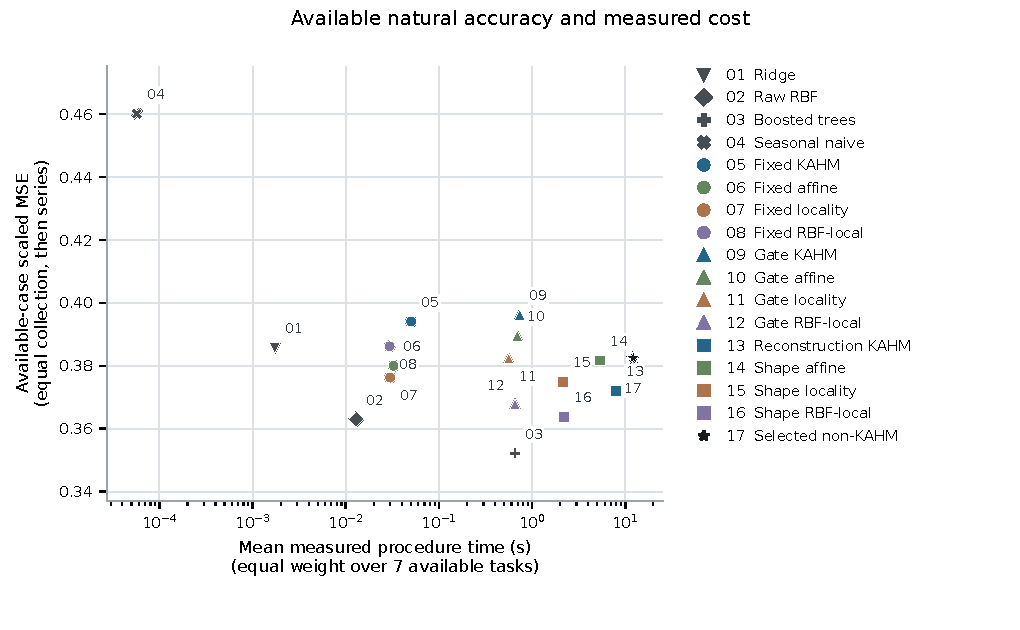
\includegraphics[width=\linewidth]{generated/direct_reconstruction/natural_available_accuracy_cost.pdf}
\caption{Available-case natural accuracy and implemented cost for all
17 procedures. Accuracy averages equally across three collections; time
averages equally across seven feasible task suites, with a logarithmic
horizontal scale. The missing rideshare collection is not replaced.
This descriptive plot does not establish population uncertainty or an
application-specific acceptable-cost threshold.}
\label{fig:direct-natural-cost}
\end{figure}
\FloatBarrier

\FloatBarrier
\section{Online adaptation: protocol and resource measurements}
\label{app:adaptive-development}

\paragraph{Inputs and temporal roles.}
The eight synthetic streams contain 2,048 retained observations each, after
256 regime-A burn-in observations. Four seeds, 20261101--20261104, pair
stationary and recurring schedules by innovations. Histories and horizons
are respectively 12 and $(1,4,12)$. The retained Dominick series T7830,
T25851 and T108533 each contain 393 weekly observations, with histories 52
and horizons $(1,2,4)$. The Sunspot input is the finite final 4,096-point
crop of the previously selected daily T1 series, starting at original raw
index 69,828; histories are 28 and horizons $(1,3,7)$. No interpolation is
used. The source archives and version identifiers are documented with the
reproduction materials \citep{Godahewa2021Monash}.

At observation time $t$, the evaluator scores previously issued forecasts
whose targets mature at $t$, releases the newly available labels, updates
the model, then issues forecasts for $t+h$. Initial fitting uses common
joint-horizon complete rows, and calibration weights are selected before
processing the first evaluation observation using only earlier targets.
Matured earlier evaluation labels may update the model; the update rule and
selected weights remain fixed. The model therefore uses labels from earlier evaluation times once
they become available, while the update algorithm remains fixed. Scale factors use the fitting
prefix only. Losses average origins within horizon, horizons within series,
then series within collection; Dominick and Sunspot receive equal weight.
The four seeds define independent simulation replications; forecasts
from overlapping windows within a stream are dependent. No broad transfer intervals
are claimed from the two selected natural collections.

\paragraph{Reference policy and calibration scope.}
The geometric bank contains four local models of rank at most two. Every
16 observations, an adaptive arm considers one local model in round-robin
order, retains half its initial references as anchors, and replaces at most
four other references with observed histories assigned to that local model.
The affected geometry and all residual heads are rebuilt coherently from
their bounded replay. No bandwidth, penalty, history, reference-policy or
refresh search is performed. The kernel comparator uses an initial-prefix
median-distance bandwidth, regularizer 0.1 and FIFO supports, with recorded
inverse-residual checks and rebuilds. Calibration selects only the four
possible horizon-specific correction weights stated in
Section~\ref{sec:adaptive-development}.
For the kernel comparator, the correction is its kernel forecast minus
the common raw ridge forecast. The same calibration rule therefore selects
a ridge--KRR mixture for each horizon: weights one and zero recover KRR
and ridge, respectively. All reported method losses include this selection.

\paragraph{Prespecified accuracy and service criteria.}
The decision to expand the evaluation requires one capacity setting
to satisfy all accuracy and service criteria. On recurring
streams, adaptive KAHM must reduce mean loss by at least 3\% against each
of adaptive affine, adaptive RBF-local and kernel ridge, with wins on at
least three of four paired seeds against each, and by at least 1\% against
both fixed KAHM and raw ridge. On the natural aggregate, it must improve
each of the three main comparators by at least 1\%; at least one collection must show improvements of at least 3\%
against all three comparators, and neither collection may be more
than 5\% worse than any. KAHM must also meet the per-stream 99th-percentile service-time screen,
with no unexpected exception or cap violation in any method. These
thresholds were fixed before the original run and were also used for
the repeated evaluation after the numerical amendment, designated A1.
Neither capacity setting meets the recurring-stream accuracy criteria.
The protocol therefore classifies both settings as insufficient for
expanding the experiment. Every criterion is evaluated within a single
capacity setting.

% Generated from saved task-level resource measurements.
\begin{table}[!htbp]
\centering\small\setlength{\tabcolsep}{5pt}
\caption{Measured service and state by method/tier. P99 denotes the 99th percentile and is first computed per stream, then maximized across the 12 streams. Other columns also report maxima; they may occur on different streams. Owned NumPy buffers exclude Python objects and temporary work arrays; worker resident set size (RSS) includes interpreter, libraries and evidence storage. Neither is a precise incremental deployment footprint.}
\label{tab:adaptive-development-resources}
\begin{tabular}{@{}llrrrr@{}}
\toprule
Method & Tier & P99 (ms) & Max (ms) & NumPy (KiB) & RSS (MiB) \\
\midrule
Raw ridge & Small & 0.55 & 1.77 & 300.34 & 150.48 \\
Raw ridge & Large & 1.26 & 4.54 & 465.72 & 150.48 \\
Fixed KAHM & Small & 4.98 & 29.01 & 466.29 & 150.48 \\
Fixed KAHM & Large & 8.61 & 27.24 & 685.38 & 150.48 \\
Adaptive KAHM & Small & 9.89 & 49.10 & 518.95 & 150.48 \\
Adaptive KAHM & Large & 11.75 & 23.60 & 824.52 & 150.48 \\
Adaptive affine & Small & 9.56 & 24.75 & 509.83 & 150.48 \\
Adaptive affine & Large & 7.00 & 13.44 & 791.39 & 150.48 \\
Adaptive RBF-local & Small & 5.05 & 12.05 & 509.83 & 150.48 \\
Adaptive RBF-local & Large & 4.58 & 8.00 & 791.39 & 150.48 \\
Sliding-window KRR & Small & 3.15 & 3.95 & 477.34 & 150.48 \\
Sliding-window KRR & Large & 3.42 & 13.49 & 1011.72 & 150.48 \\
\bottomrule
\end{tabular}
\end{table}


\paragraph{Resource scope.}
Workers execute serially in fresh processes with one numerical thread and
the same CPU affinity. Initialization and calibration are measured
separately. The service interval covers history/pair assembly, all matured
horizon updates, feature/head rebuilds, kernel inverse audits and prediction;
scoring, serialization and state inspection are excluded. Buffer-state
samples and whole-worker peak RSS have the distinct scopes stated in
Table~\ref{tab:adaptive-development-resources}. The 20\,ms allowance is a
host-specific engineering screen, not an application-derived service-level
requirement. Different support sharing across horizons prevents interpreting
the tier labels as equal memory or equal computation.

\paragraph{Solver amendment and computational verification.}
The original implementation accumulated correction cross-products;
large rows entering and leaving a finite window produced cancellation in
the reproduced failing state. The amended implementation (A1) recomputes residuals against the
current baseline from the same bounded replay, centers to eliminate the
free intercept, equilibrates both data and penalty columns, and solves
the augmented ridge objective with pivoted QR. It changes arithmetic, not
the specified objective or advancement rule. The original 144 runs remain
in \path{extensions/adaptive_development/archives/initial_attempt.zip}.
Because the amended runs repeat the same inputs, they do not increase
the number of independent experimental replications. The verification program passes
\ADAuditChecks{} computational consistency checks, covering chronology,
coverage, calibration selection, aggregation, decision gates, resources,
shared baselines and matched reference changes. It imports neither the
forecasting model nor its analyzer, but remains an internal computational
check rather than independent scientific replication.

The reproduction materials contain both versions of the protocol and
source, the numerical diagnostic states, input hashes, predictions,
update traces, and summaries. The manuscript builder
\path{extensions/tmlr_integration/build_adaptive_assets.py} reconstructs
the displayed collection means and resource maxima from saved task
records, checks them against the analysis and decision files, and records
input/output hashes. It performs no model fitting. Both execution checkpoints were recorded locally. The study was not
publicly preregistered.

\FloatBarrier
\section{Reconstruction algebra and bounded residual decoding}
\label{app:reconstruction-mechanism}

This appendix analyzes fixed reference maps and their use by a specified
decoder. It establishes normalized-kernel identities, conditions for equality
or inequality of feature spans, and a bound on fitted residual corrections.
None of these statements assumes a particular time-series distribution or
guarantees a forecasting improvement. Unless another subscript is displayed,
vector norms are Euclidean norms. The numerical examples can be evaluated
with \path{extensions/reconstruction_mechanism/algebra.py}; their reference
banks are constructed independently of forecasting outcomes.

\subsection{Normalized kernel identities}

Let $q_1,\ldots,q_M\in\R^d$ be reference histories, and let
$Q\in\R^{M\times d}$ contain their transposes as rows. Let
$P\in\R^{d\times r}$ have orthonormal columns, with $1\leq r\leq d$,
and let $W\in\R^{r\times r}$ be a symmetric positive-definite precision
matrix for the projected coordinates. For a column-vector query
$x\in\R^d$, define the Gaussian kernel vector $k(x)\in\R^M$ by
\[
 k_i(x)=\exp\!\left[-\frac{
 (P^\top(x-q_i))^\top W(P^\top(x-q_i))}{2r}\right],
 \qquad i=1,\ldots,M.
\]
Let $K\in\R^{M\times M}$ be the reference Gram matrix, with
$K_{ij}=k_i(q_j)$. For $\lambda>0$, set
$C=(K+\lambda I_M)^{-1}$, where $I_M$ is the $M\times M$ identity
matrix, and let $\mathbf1_M$ be the length-$M$ vector of ones.
The matrix $K$ is symmetric positive semidefinite, so $C$ exists and is
symmetric positive definite. The KAHM and matched positive-kernel
reconstructions are
\begin{equation}
 A_K(x)=\frac{Q^\top Ck(x)}{\mathbf1_M^\top Ck(x)},\qquad
 A_R(x)=\frac{Q^\top k(x)}{\mathbf1_M^\top k(x)}.
 \label{eq:mechanism-normalized-maps}
\end{equation}
The first expression is defined wherever its signed denominator is nonzero.
The second denominator is positive for every finite query. The two maps
share the references and projected Gaussian kernel. Multiplying $k(x)$
by a common positive scalar cancels in either ratio, which justifies
subtracting the largest log-kernel value before query evaluation.

\begin{proposition}[Normalization and target transfer]
\label{prop:mechanism-krr}
For a query satisfying $s(x)=\mathbf1_M^\top Ck(x)\ne0$, define the
normalized weight vector $\alpha(x)=Ck(x)/s(x)$. Its entries sum to one.
For any reference target vector $y\in\R^M$,
\[
 \alpha(x)^\top y=
 \frac{k(x)^\top(K+\lambda I_M)^{-1}y}
 {k(x)^\top(K+\lambda I_M)^{-1}\mathbf1_M}.
\]
Thus target transfer is the ratio of two dual kernel-ridge predictions
with regularization matrix $K+\lambda I_M$ and no additional intercept:
one fitted to $y$, and one fitted to the constant target $\mathbf1_M$.
For an affine scalar function $f(q)=q^\top b+c$, with
$b\in\R^d$ and $c\in\R$, let $f(Q)=Qb+c\mathbf1_M$ be its reference
values. Then
\[
 \alpha(x)^\top f(Q)-f(x)=\{A_K(x)-x\}^\top b.
\]
\end{proposition}
\begin{proof}
The definition gives
$\mathbf1_M^\top\alpha(x)=s(x)/s(x)=1$. Because $C=C^\top$,
$\alpha(x)^\top y=k(x)^\top Cy/s(x)$ and
$s(x)=k(x)^\top C\mathbf1_M$, proving the ratio identity.
For the affine function,
\[
 \alpha(x)^\top f(Q)
 =\alpha(x)^\top Qb+c\alpha(x)^\top\mathbf1_M
 =A_K(x)^\top b+c.
\]
Subtracting $x^\top b+c$ proves the final identity.
\end{proof}

This identifies direct target transfer as a normalized kernel-ridge
construction. The ratio generally differs from the unnormalized
kernel-ridge predictor because its denominator depends on the query.
Similarly, $A_K(x)^\top b$ is normalized kernel ridge applied to the
restricted reference target $Qb$. For any reconstruction $A$, the identity
$A(x)+\{x-A(x)\}=x$ also implies a linear dependence among the raw input,
reconstruction, and residual when all three are included as unrestricted
linear features. These identities constrain claims about the resulting
function class while allowing useful parameterizations for a restricted
or regularized decoder.

\subsection{When reconstruction departures have the same span}

Let $\mu\in\R^d$ be the reference center and define the affine
reconstruction $A_A(x)=\mu+PP^\top(x-\mu)$. Fix a common scalar locality
gate $g(x)$, and define column-vector departures
\[
 d_K(x)=g(x)\{A_K(x)-A_A(x)\},\qquad
 d_R(x)=g(x)\{A_R(x)-A_A(x)\}.
\]
A feature span means the set of scalar functions obtained by finite linear
combinations of its coordinate functions. Let $\mathcal S_0$ be the span
of the gate $g(x)$ and the coordinates of $g(x)P^\top(x-\mu)$.
It contains every coordinate of $g(x)A_A(x)$.

\begin{proposition}[A sufficient condition for equal feature spans]
\label{prop:mechanism-redundancy}
Suppose $K\mathbf1_M=\kappa\mathbf1_M$ for a scalar $\kappa$ and
$C$ leaves the augmented reference-coordinate space
$\mathcal V=\operatorname{span}\{\mathbf1_M,Q_{:1},\ldots,Q_{:d}\}
\subseteq\R^M$ invariant. Here $Q_{:j}$ denotes column $j$ of $Q$.
Then there exist $B\in\R^{d\times d}$ and $c\in\R^d$ such that
\[
 C\mathbf1_M=a\mathbf1_M,\qquad
 CQ=QB+\mathbf1_M c^\top,\qquad a=(\kappa+\lambda)^{-1}>0.
\]
For these coefficients,
\[
 A_K=\frac{B^\top A_R+c}{a},\qquad
 d_K=\frac{B^\top}{a}d_R+
 \left(\frac{B^\top}{a}-I_d\right)gA_A+\frac{gc}{a}.
\]
The span obtained by adjoining the coordinates of $d_K$ to
$\mathcal S_0$ is the same as that obtained by adjoining the coordinates
of $d_R$.
\end{proposition}
\begin{proof}
The constant-row-sum assumption implies
$(K+\lambda I_M)\mathbf1_M=(\kappa+\lambda)\mathbf1_M$,
so $C\mathbf1_M=a\mathbf1_M$. Since $K$ is positive semidefinite,
$\kappa\geq0$ and hence $a>0$. Invariance of $\mathcal V$ means each
column of $CQ$ can be expressed using $Q$ and $\mathbf1_M$, which gives
$B$ and $c$. Using symmetry of $C$ in
Equation~\eqref{eq:mechanism-normalized-maps},
\[
 A_K(x)=
 \frac{(CQ)^\top k(x)}{(C\mathbf1_M)^\top k(x)}
 =\frac{B^\top Q^\top k(x)+c\mathbf1_M^\top k(x)}
 {a\mathbf1_M^\top k(x)}
 =\frac{B^\top A_R(x)+c}{a}.
\]
Subtract $A_A$ and multiply by $g$ to obtain the displayed departure
identity. Since $gA_A=g\mu+P\{gP^\top(x-\mu)\}$, all its coordinates
belong to $\mathcal S_0$. Thus the KAHM-augmented span is contained in
the RBF-augmented span.

For the reverse inclusion, the restriction of the invertible matrix $C$
to the invariant finite-dimensional space $\mathcal V$ is injective and
therefore surjective onto $\mathcal V$. Its images
$C\mathbf1_M=a\mathbf1_M$ and the columns of $CQ$ consequently span
$\mathcal V$. Hence there exist $D\in\R^{d\times d}$ and $e\in\R^d$ such that
$Q=(CQ)D+\mathbf1_M e^\top$. Multiplying its transpose by
$k(x)/(\mathbf1_M^\top k(x))$ gives
$A_R(x)=aD^\top A_K(x)+e$. After multiplication by $g$ and subtraction
of $gA_A$, this expresses each RBF departure coordinate using KAHM
departure coordinates and $\mathcal S_0$. The spans therefore agree,
including when the original reference-coordinate columns are redundant.
\end{proof}

For example, take scalar references $q=(-1,1)^\top$, $P=1$, $g=1$,
and $A_A(x)=x$. If the off-diagonal Gram entry is $\rho$, then
$K\mathbf1_2=(1+\rho)\mathbf1_2$ and $Kq=(1-\rho)q$. Therefore
\begin{equation}
 A_K=c_\rho A_R,\qquad
 d_K=c_\rho d_R+(c_\rho-1)x,\qquad
 c_\rho=\frac{1+\rho+\lambda}{1-\rho+\lambda}.
 \label{eq:mechanism-two-reference}
\end{equation}
The coefficient $c_\rho$ is positive, so
$\operatorname{span}(1,x,d_K)=\operatorname{span}(1,x,d_R)$.
With the sample-variance precision $1/2$, $\rho=e^{-1}$.
The regularization iteration used by the implementation yields
$\lambda=2.6519665429866075$ and $c_\rho=1.224037566462905$.
The maximum numerical identity error on the constructed query grid is
below $6\times10^{-16}$.

These are equalities between untransformed feature spans. An isotropic
ridge penalty is not invariant under a general nonorthogonal change of
coordinates. Applying separate nonlinear radial transformations can also
remove the displayed linear relation. A forecasting comparison therefore
evaluates the complete reconstruction, feature transformation, and fitting
procedure, even when two untransformed feature sets have the same span.

\subsection{An explicit distinct reconstruction basis}

\begin{proposition}[Irregular scalar references]
\label{prop:mechanism-distinct}
Let $q_1<q_2<q_3$ with $q_1+q_3\ne2q_2$, and define
$k_i(x)=\exp\{-t(x-q_i)^2/2\}$ for precision $t>0$.
Let $K_{ij}=\exp\{-t(q_i-q_j)^2/2\}$,
$C=(K+\lambda I_3)^{-1}$ for $\lambda>0$, and suppose every entry of
$v=C\mathbf1_3$ is positive. For the reconstructions in
Equation~\eqref{eq:mechanism-normalized-maps}, with $Q=q=(q_1,q_2,q_3)^\top$,
gate $g=1$, and $A_A(x)=x$,
\[
 A_K\notin\operatorname{span}(1,x,A_R),\qquad
 d_K\notin\operatorname{span}(1,x,d_R).
\]
These are statements about scalar functions on the whole real line.
\end{proposition}
\begin{proof}
Set $u=Cq$. Since $C$ is symmetric,
$A_K(x)=(k(x)^\top u)/(k(x)^\top v)$, and positivity of $v$ makes
its denominator positive for every $x$. The six sums $q_i+q_j$ with
$i\leq j$ are distinct: strict ordering of the three references orders
all the sums except possibly $q_1+q_3$ and $2q_2$, and their equality
is excluded by assumption. Products of Gaussian translates satisfy
\[
 k_i(x)k_j(x)=
 e^{-tx^2}e^{-t(q_i^2+q_j^2)/2}e^{t(q_i+q_j)x}.
\]
After removal of the common positive factor $e^{-tx^2}$, these products
are nonzero multiples of exponentials with six distinct real exponents.
Such exponentials are linearly independent. Indeed, differentiating a
vanishing linear combination zero through fifth order at $x=0$ gives
a Vandermonde system whose determinant is the product of the nonzero
pairwise exponent differences.

Suppose first that $A_K=cA_R+d$ for scalars $c,d$. Define
$w=u-dv$. Multiplication by the two positive denominators gives
\[
 \left(\sum_i k_iw_i\right)\left(\sum_j k_j\right)
 =c\left(\sum_i k_iq_i\right)\left(\sum_j k_jv_j\right).
\]
Independence of the six products implies equality of their coefficients.
The diagonal coefficients give $w_i=cq_iv_i$, and the off-diagonal
coefficients give
$w_i+w_j=c(q_iv_j+q_jv_i)$ for $i<j$.
If $c=0$, all $w_i$ vanish, so $Cq=dC\mathbf1_3$. Invertibility of
$C$ would imply $q=d\mathbf1_3$, contrary to the distinct references.
If $c\ne0$, substituting the diagonal equations into the off-diagonal
ones yields $(q_i-q_j)(v_i-v_j)=0$. Thus $v=a\mathbf1_3$ for some
$a>0$, and $(K+\lambda I_3)v=\mathbf1_3$ implies that $K$ has
constant row sums. This is impossible: its middle-row sum exceeds the
first-row sum by $K_{23}-K_{13}>0$ and the last-row sum by
$K_{12}-K_{13}>0$, since the Gaussian decreases strictly with positive
distance. This rules out every affine relation $A_K=cA_R+d$.

Both reconstructions are bounded functions of $x$. The RBF reconstruction
is a convex combination of $q_1,q_2,q_3$. Also,
\[
 A_K(x)=\frac{\sum_i k_i(x)v_i\,(u_i/v_i)}
 {\sum_i k_i(x)v_i}
\]
is a convex combination of the three finite numbers $u_i/v_i$.
If $A_K=cA_R+d+bx$ held on the real line, boundedness of both
reconstructions would force $b=0$. The affine relation already ruled out
would then follow. This proves the first span statement. Finally,
$d_K=A_K-x$ and $d_R=A_R-x$ imply
$\operatorname{span}(1,x,d_R)=\operatorname{span}(1,x,A_R)$.
Membership of $d_K$ in this span would imply membership of $A_K$, a
contradiction.
\end{proof}

A concrete example uses $q=(-1,0,2)^\top$, sample-variance precision
$t=3/7$, and $\lambda=4.498274743339644$ from the specified
regularization iteration. Positivity of $C\mathbf1_3$ can be verified
without examining a query grid. Write $K=I_3+E$ and $a=1+\lambda$.
For a matrix, let $\|\cdot\|_\infty$ denote the maximum absolute row
sum; for a vector, it denotes the largest absolute entry. If
$a>2\|E\|_\infty$, then the Neumann series for
$aC=(I_3+E/a)^{-1}$ gives
\[
 \|aC\mathbf1_3-\mathbf1_3\|_\infty
 \leq\sum_{j=1}^{\infty}(\|E\|_\infty/a)^j
 =\frac{\|E\|_\infty/a}{1-\|E\|_\infty/a}<1.
\]
Every entry of $aC\mathbf1_3$ is then strictly positive. In the example,
$\|E\|_\infty=e^{-3/14}+e^{-6/7}=1.2314905926823394$, so the
condition holds. On $81$ constructed queries in $[-3,4]$, the maximum
absolute residual after least-squares projection of the sampled $d_K$
values onto the sampled $(1,x,d_R)$ columns is
$0.05355670997078987$. This numerical illustration supplements the
analytic existence result. It does not establish distinctness for every
higher-dimensional bank used in the forecasting experiments.

\subsection{A bounded correction with a free intercept}

For a feature block $v\in\R^{p_b}$ of positive width $p_b$, define
\begin{equation}
 T_{R_b}(v)=\frac{v}{\sqrt{1+\|v\|_2^2/R_b^2}},\qquad
 R_b=\sqrt{p_b}.
 \label{eq:mechanism-radial}
\end{equation}
Its norm is at most $R_b$. To see its sensitivity to its own input, set
$a=1+\|v\|_2^2/R_b^2$. Its Jacobian is
$a^{-1/2}I-a^{-3/2}vv^\top/R_b^2$. For $v\ne0$, the eigenvalue in
the direction of $v$ is $a^{-3/2}$, and each orthogonal direction has
eigenvalue $a^{-1/2}$; at zero, the Jacobian is the identity. All its
singular values are therefore at most one. Integrating the derivative
along the segment between any two inputs proves
$\|T_{R_b}(v)-T_{R_b}(v')\|_2\leq\|v-v'\|_2$.
Thus the radial transformation is nonexpansive.

Concatenating separately transformed blocks gives a feature vector
$\psi(x)\in\R^p$, where $p=\sum_b p_b$, satisfying
$\|\psi(x)\|_2\leq R=(\sum_bR_b^2)^{1/2}$. This norm bound holds
wherever the preceding feature construction is defined. Nonexpansiveness
of the radial transformation does not by itself give a Lipschitz constant
for the full history-to-feature map, which includes the signed
reconstruction denominator and its fallback rule.

\begin{proposition}[Centered ridge correction bound]
\label{prop:mechanism-correction-bound}
For $n\geq1$, let $e_i\in\R$ be residual targets and
$\psi_i\in\R^p$ be training feature vectors. Fit $b\in\R$ and
$w\in\R^p$ by minimizing
\[
 \frac1n\sum_{i=1}^n(e_i-b-\psi_i^\top w)^2+\alpha\|w\|_2^2,
 \qquad\alpha>0,
\]
with no penalty on $b$. Define the training means
$\bar e=n^{-1}\sum_i e_i$ and
$\bar\psi=n^{-1}\sum_i\psi_i$, the residual vector
$e=(e_1,\ldots,e_n)^\top$, its centered version
$e_c=e-\bar e\mathbf1_n$, and its centered root mean square
$\sigma_e=\|e_c\|_2/\sqrt n$. Suppose query features satisfy
$\|\psi(x)\|_2\leq R$. Then, for any scalar $\gamma$,
\begin{equation}
 \|w\|_2\leq\frac{\sigma_e}{2\sqrt\alpha},\qquad
 |\gamma q(x)|\leq|\gamma|\left[
 |\bar e|+(R+\|\bar\psi\|_2)\frac{\sigma_e}{2\sqrt\alpha}\right],
 \quad q(x)=\bar e+(\psi(x)-\bar\psi)^\top w.
 \label{eq:mechanism-correction-bound}
\end{equation}
\end{proposition}
\begin{proof}
For fixed $w$, differentiating with respect to the intercept gives
$b=\bar e-\bar\psi^\top w$. Let $\Psi_c\in\R^{n\times p}$ have
row $i$ equal to $(\psi_i-\bar\psi)^\top$. Substituting the fitted
intercept reduces the objective to
$n^{-1}\|e_c-\Psi_cw\|_2^2+\alpha\|w\|_2^2$.
Its unique minimizer is
\[
 w=(\Psi_c^\top\Psi_c+n\alpha I_p)^{-1}\Psi_c^\top e_c.
\]
For a singular value $s\geq0$ of $\Psi_c$, the corresponding singular
value of the coefficient operator is $s/(s^2+n\alpha)$. The inequality
$(s-\sqrt{n\alpha})^2\geq0$ implies
\[
 \frac{s}{s^2+n\alpha}\leq\frac{1}{2\sqrt{n\alpha}}.
\]
The operator norm is therefore at most $1/(2\sqrt{n\alpha})$, giving
$\|w\|_2\leq\|e_c\|_2/(2\sqrt{n\alpha})
=\sigma_e/(2\sqrt\alpha)$. Finally, the fitted intercept gives
$q(x)=\bar e+(\psi(x)-\bar\psi)^\top w$.
Cauchy--Schwarz and the triangle inequality yield
\[
 |q(x)|\leq|\bar e|+
 (\|\psi(x)\|_2+\|\bar\psi\|_2)\|w\|_2
 \leq|\bar e|+(R+\|\bar\psi\|_2)
 \frac{\sigma_e}{2\sqrt\alpha}.
\]
Multiplication by $|\gamma|$ proves the correction bound.
\end{proof}

The mean-squared-error objective corresponds to a summed-squared-error
objective with penalty $n\alpha$. Keeping the numerical value $\alpha$
unchanged when switching to a summed loss would define a different
estimator. For multiple forecast horizons, the bound applies separately
to each fitted residual vector and each selected pair
$(\alpha_h,\gamma_h)$. This is a general property of ridge regression
on bounded features, including the KAHM features considered here. It
bounds the additive correction but does not bound the retained raw
baseline or total forecast error. The experiment checks the feature,
coefficient, and correction inequalities on every saved task and reports
forecast errors separately.

\FloatBarrier
\section{Complete reconstruction-departure evaluation}
\label{app:reconstruction-results}

This appendix gives the numerical observation protocol, full method roster,
descriptive condition results, stability accounting, selection frequencies
and measured resources for Section~\ref{sec:reconstruction-mechanism}.
The frozen implementation and complete arrays are under
\path{extensions/reconstruction_mechanism}. All displays are generated
from the completed independent analysis; their source and output hashes are
recorded in
\path{generated/reconstruction_mechanism/ASSET_PROVENANCE.json}.

\subsection{Observation laws and separation of roles}

The linear negative control is
\[
 y_t=0.65y_{t-1}-0.15y_{t-2}+\epsilon_t,
 \qquad \epsilon_t\stackrel{\mathrm{iid}}\sim\mathcal N(0,0.1^2),
\]
with two initial zeros, 256 discarded stored values and 72 retained values
beginning at $y_{256}$. The nonlinear AR uses
\[
 y_t=\tanh\{1.25y_{t-1}-0.65y_{t-2}
             +0.25\sin(3y_{t-1})+u_t\},
 \qquad u_t\stackrel{\mathrm{iid}}\sim U[-0.1,0.1],
\]
two initial values uniform on $[-0.8,0.8]$, and 80 discarded stored values.
Van der Pol uses $\dot x=v$, $\dot v=(1-x^2)v-x$; Duffing uses
$\dot x=v$, $\dot v=-0.2v+x-x^3+0.3\cos(1.2t+\varphi)$.
The inherited float64 RK4 implementation has step 0.025, observation interval
0.1 and burn time ten. Initial $x,v$ are independent uniform on $[-2,2]$;
$\varphi$ is uniform on $[0,2\pi]$. Oscillator observations are
$0.95\tanh(x)+U[-0.02,0.02]$. The numerical integrator and observation
map define the tested laws; they are not exact continuous-ODE trajectories.

For each law and repetition, all split episodes are generated once. Additional
noise is $\eta s_A Z$, with $\eta\in\{0,0.1\}$,
$Z\stackrel{\mathrm{iid}}\sim\mathcal N(0,1)$ and $s_A$ the population
standard deviation of all unaugmented observed A episode values. Underlying
episodes and $Z$ arrays are paired across the two levels. The noise changes
both input histories and forecast targets. At zero added noise, the inherited
oscillator sensor noise remains. On B/C/D, the augmented linear observations are Gaussian conditional
on the realized A-estimated amplitude; across repetitions that random
amplitude induces a variance mixture. Neither exact stationarity after
finite burn-in nor a known-amplitude oracle interpretation of fitted ridge
is assumed. The Gaussian additions also preclude carrying over a bounded-loss
claim from the earlier bounded observation studies.

The 24 repetition seeds are 946100--946123. Development seed 975001 is
excluded. A/B/C/D base episodes and unit-noise arrays are generated from
distinct independent random streams; the added-noise amplitude is estimated
from A and shared across splits. Row caps and fitting seeds are paired between noise
levels. All 13 within-episode origins, at indices $11,15,\ldots,59$, use only
history through their origin and target offsets $(1,4,12)$. There are
\RMTargetCells{} scored target cells per method across the complete roster,
but only 24 independent aggregates in the primary inference. No individual
origin, horizon or paired-noise task is promoted to an independent replicate.

A fits every scaler, reference bank, kernel factor, raw predictor and decoder.
B selects model settings separately for each horizon. C selects each
non-ridge mixing coefficient, then one whole non-KAHM procedure. Selected
states are serialized before reserved queries are passed to prediction, and
targets enter the execution wrapper only after forecasts have been fixed.
No parameter or selection is updated on D.

\subsection{Fixed settings and complete descriptive losses}

The common locality logit is
$-\|z-\mu_j\|^2/(2s_j)$, where $s_j$ is the inherited mean squared
local radius, floored at $10^{-6}$. Softmax normalization occurs separately
within the 2-, 4- and 8-model blocks. Principal rank is two, there are at most
24 references per local model, and the A bank cap is 512 rows. The inherited
KAHM reference-energy regularization is unchanged. Reference and query kernels
use the same projected covariance precision; the query log-kernel maximum is
subtracted before exponentiation for both KAHM and positive RBF ratios.

The inherited history scaler replaces standard deviations at or below
$10^{-12}$ by one. The subsequent A feature scalers use
$\max(\mathrm{sd},10^{-6})$. Raw ridge/RBF history scalers also use this
$10^{-6}$ floor. Common and departure blocks are radially bounded separately,
with no scaling after the transform. The unbounded ablations retain the same
bounded common block and omit only the departure radial map. Their failures
or successes cannot replace the bounded primary candidate.

Every ridge head uses the mean-SSE objective and the five penalties
$10^{-4},10^{-3},10^{-2},10^{-1},1$. The equivalent sum-SSE penalty is
$n\alpha$, not $\alpha$. The raw RBF arm concatenates standardized histories
with at most 64 Nystr\"om coordinates, then scales those concatenated columns
using A alone. Bandwidth factors 0.5, 1 and 2 multiply the median positive
landmark squared-distance scale; B selects bandwidth and penalty separately
by horizon. Histogram gradient boosting uses 100 iterations, L2 penalty one,
learning rates 0.05 or 0.1 and maximum leaves 7 or 15; B again selects separately
by horizon. Persistence repeats the latest observed value before its common
baseline mixing step. All non-ridge procedures use the same C mixing grid
$\{0,1/4,1/2,1\}$, with deterministic tie order.

\begin{table}[!htbp]
\centering\scriptsize
\setlength{\tabcolsep}{3pt}
\caption{All ten procedures, every declared law and both added-noise levels.
Entries are mean horizon-averaged A-variance-normalized D MSE over 24
repetitions; lower is better. The first six columns enter the nonlinear
aggregate with equal weight. The final two form the separate linear control.
These conditionwise summaries are descriptive. ``Unbounded'' omits only the
departure radial bound. Persistence and raw nonlinear controls include their
C-selected blend with ridge.}
\label{tab:mechanism-all-methods}
% Generated from the complete saved reconstruction-mechanism analysis.
\begin{tabular}{@{}lrrrrrrrr@{}}
\toprule
Procedure & \multicolumn{2}{c}{Nonlinear AR} & \multicolumn{2}{c}{Van der Pol} & \multicolumn{2}{c}{Duffing} & \multicolumn{2}{c}{Linear AR} \\
\midrule
Added noise $\eta$ & 0 & 0.1 & 0 & 0.1 & 0 & 0.1 & 0 & 0.1 \\
Raw ridge & 0.0216 & 0.0344 & 0.0750 & 0.1361 & 0.0192 & 0.0681 & 0.8951 & 0.8975 \\
Raw RBF & 0.0197 & 0.0323 & 0.0131 & 0.0647 & 0.0129 & 0.0442 & 0.8969 & 0.8994 \\
Boosted trees & 0.0201 & 0.0323 & 0.0040 & 0.0586 & 0.0133 & 0.0481 & 0.8975 & 0.8997 \\
Persistence blend & 0.0219 & 0.0345 & 0.0750 & 0.1362 & 0.0192 & 0.0684 & 0.8955 & 0.8988 \\
Common basis & 0.0190 & 0.0310 & 0.0251 & 0.0686 & 0.0157 & 0.0460 & 0.8959 & 0.8983 \\
KAHM departure (bounded) & 0.0192 & 0.0314 & 0.0101 & 0.0622 & 0.0129 & 0.0439 & 0.8972 & 0.8990 \\
RBF departure (bounded) & 0.0189 & 0.0309 & 0.0115 & 0.0634 & 0.0133 & 0.0436 & 0.8968 & 0.8989 \\
KAHM departure (unbounded) & 0.0198 & 0.0321 & 0.0108 & 0.0619 & 0.0129 & 0.0440 & 0.8975 & 0.8995 \\
RBF departure (unbounded) & 0.0190 & 0.0310 & 0.0118 & 0.0627 & 0.0127 & 0.0437 & 0.8972 & 0.8993 \\
C-selected non-KAHM policy & 0.0192 & 0.0312 & 0.0040 & 0.0590 & 0.0127 & 0.0434 & 0.8978 & 0.8997 \\
\bottomrule
\end{tabular}

\end{table}

The machine-readable files \texttt{horizon\_metrics.csv} and
\texttt{condition\_horizon\_metrics.csv} retain every method, law, noise
level and horizon, including raw MSE and the A-only loss scale. They are not
pooled with historical losses that use different normalizations. The
\texttt{replicate\_contrasts.csv} file contains all 24 margin-gap values for
each primary contrast, allowing the six lower bounds to be recomputed without
importing any forecasting model.

\subsection{Stability, numerical safeguards and correction activation}

The bounded-feature checks cover 192 tasks for each of three bounded
procedures. Coefficient and correction checks additionally distinguish the
three horizons, giving 576 checks per procedure for each inequality. The
independent analyzer checks the recorded fitted-state bound formulas and
recomputes actual D corrections as the saved forecast minus the saved raw
ridge forecast. It does not claim to reconstruct the fitted coefficient
matrices from summary statistics alone. Table~\ref{tab:mechanism-bounds}
reports maxima over the complete roster; maxima in different columns need
not come from the same task or horizon.

\begin{table}[!htbp]
\centering\small
\setlength{\tabcolsep}{5pt}
\caption{Observed ratios to the deterministic bounded-feature and
ridge-readout limits. Feature ratios concern the common block for the
common procedure and the respective departure block for the two appended
procedures; the readout bound uses the complete concatenated feature radius.
A zero correction with a zero bound contributes ratio zero. ``Violations''
sums failed feature, coefficient and correction checks at the fixed numerical
tolerances. These are implementation checks, not confidence intervals for
forecast risk.}
\label{tab:mechanism-bounds}
% Generated from the complete saved reconstruction-mechanism analysis.
\begin{tabular}{@{}lrrrr@{}}
\toprule
Bounded procedure & \shortstack{Feature norm\\/ radius} & \shortstack{Coefficient norm\\/ bound} & \shortstack{Correction\\/ bound} & Violations \\
\midrule
Common basis & 0.99493 & 0.56103 & 0.29634 & 0 \\
KAHM departure (bounded) & 0.99943 & 0.55231 & 0.20110 & 0 \\
RBF departure (bounded) & 0.99734 & 0.44963 & 0.19674 & 0 \\
\bottomrule
\end{tabular}

\end{table}

The maximum taskwise ratio of KAHM maximum absolute error to ridge maximum
absolute error is \RMMaxErrorRatio{}, and \RMStabilityFailures{} tasks fail
at least one declared stability screen. Local KAHM reconstruction fallback
affects \RMKFallbackABC{} A/B/C rows and \RMKFallbackD{} D rows across all
tasks; the corresponding RBF D count is \RMRFallbackD{}. Counts are unions
over local models within a task and split, so the same row is not counted
again merely because several local maps invoke their guard. The fixed local
fallback sets the affected departure to zero. The complete valid analysis
requires zero wholly failed methods and zero final prediction-cell recoveries;
neither is hidden by removing a task or substituting a successful subset.

\begin{table}[!htbp]
\centering\small
\setlength{\tabcolsep}{4pt}
\caption{C-selected correction activation. Nonlinear and linear counts have
432 and 144 task/horizon cells, respectively. The four mixing-weight columns
combine all 576 cells. A policy choice of raw ridge is counted as zero
correction; raw ridge itself has no mixing selection. Nonzero mixing is not
an empirical guarantee of D improvement, and no minimum activation frequency
was part of the decision.}
\label{tab:mechanism-activation}
% Generated from the complete saved reconstruction-mechanism analysis.
\begin{tabular}{@{}lrrrrrr@{}}
\toprule
Procedure & \shortstack{Nonlinear\\active / 432} & \shortstack{Linear\\active / 144} & $\gamma=0$ & $\gamma=1/4$ & $\gamma=1/2$ & $\gamma=1$ \\
\midrule
Raw ridge & --- & --- & --- & --- & --- & --- \\
Raw RBF & 427 & 56 & 93 & 52 & 158 & 273 \\
Boosted trees & 396 & 48 & 132 & 106 & 175 & 163 \\
Persistence blend & 70 & 32 & 474 & 97 & 5 & 0 \\
Common basis & 430 & 56 & 90 & 9 & 66 & 411 \\
KAHM departure (bounded) & 432 & 54 & 90 & 23 & 79 & 384 \\
RBF departure (bounded) & 431 & 58 & 87 & 14 & 71 & 404 \\
KAHM departure (unbounded) & 428 & 51 & 97 & 40 & 107 & 332 \\
RBF departure (unbounded) & 429 & 61 & 86 & 26 & 75 & 389 \\
C-selected non-KAHM policy & 430 & 63 & 83 & 46 & 100 & 347 \\
\bottomrule
\end{tabular}

\end{table}

\begin{table}[!htbp]
\centering\small
\setlength{\tabcolsep}{8pt}
\caption{Whole-procedure choices made by the C-selected non-KAHM policy.
Each task contributes one choice across all horizons after each candidate's
own horizon-wise C mixing selection. Both KAHM arms are excluded. These are
validation choices, not choices made from D errors.}
\label{tab:mechanism-policy}
% Generated from the complete saved reconstruction-mechanism analysis.
\begin{tabular}{@{}lrr@{}}
\toprule
C-selected complete procedure & Nonlinear / 144 & Linear / 48 \\
\midrule
Raw ridge & 0 & 1 \\
Raw RBF & 19 & 6 \\
Boosted trees & 51 & 8 \\
Persistence blend & 2 & 20 \\
Common basis & 15 & 4 \\
RBF departure (bounded) & 19 & 1 \\
RBF departure (unbounded) & 38 & 8 \\
\bottomrule
\end{tabular}

\end{table}

\subsection{Measured costs and reproducibility limits}

\begin{table}[!htbp]
\centering\small
\setlength{\tabcolsep}{4pt}
\caption{Mean charged resources over all 192 equal-sized task suites.
Fit/select includes required A fitting, B selection and C calibration.
D prediction covers all 1,664 histories and three horizons. Shared computation
nodes are charged once to every procedure requiring them; policy fitting pays
the union of its non-KAHM candidates, while its prediction/state follow the
selected complete procedure. State denotes serialized selected objects;
arrays count their owned NumPy buffers. These are measured implementation
costs, not minimum deployment complexity.}
\label{tab:mechanism-resources}
% Generated from the complete saved reconstruction-mechanism analysis.
\begin{tabular}{@{}lrrrrr@{}}
\toprule
Procedure & \shortstack{Fit/select\\wall (s)} & \shortstack{Fit/select\\CPU (s)} & \shortstack{D predict\\wall (ms)} & \shortstack{State\\(KiB)} & \shortstack{Arrays\\(KiB)} \\
\midrule
Raw ridge & 0.0010 & 0.0010 & 0.147 & 1.10 & 0.63 \\
Raw RBF & 0.0135 & 0.0135 & 2.925 & 65.58 & 64.28 \\
Boosted trees & 0.6452 & 0.6452 & 19.046 & 373.94 & 335.61 \\
Persistence blend & 0.0011 & 0.0011 & 0.197 & 1.15 & 0.66 \\
Common basis & 0.0367 & 0.0353 & 5.363 & 9.00 & 6.82 \\
KAHM departure (bounded) & 0.0833 & 0.0819 & 29.245 & 118.81 & 114.76 \\
RBF departure (bounded) & 0.0658 & 0.0644 & 25.758 & 55.32 & 51.85 \\
KAHM departure (unbounded) & 0.0812 & 0.0798 & 26.655 & 118.81 & 114.76 \\
RBF departure (unbounded) & 0.0642 & 0.0628 & 23.810 & 55.32 & 51.85 \\
C-selected non-KAHM policy & 0.7374 & 0.7360 & 15.068 & 151.36 & 137.94 \\
\bottomrule
\end{tabular}

\end{table}

Each task runs serially in a fresh process with one assigned CPU and one
numerical thread. The charged primitive-node costs exclude diagnostic-only
rank calculations; full-suite timings, including diagnostics, are retained
separately. Node accounting includes model candidates that are actually
evaluated, rather than only the winning hyperparameters. Wall and CPU times
depend on the recorded machine and software environment. The peak whole-task
process RSS is \RMPeakProcessMiB{} MiB; it includes imports, all ten arms,
shared diagnostics and evidence arrays, and is not a per-method RAM estimate.
Serialized state and owned array buffers omit transient workspace and do not
measure online update latency. No cost ceiling was imposed without an
application-derived requirement.

The independent analyzer verifies the immutable local source/input freeze,
the complete task roster, exact target correspondence, A variance scales,
policy predictions, nonfinite/failure accounting and all primary aggregation.
The reporting builder separately reconstructs condition and repetition means
and all six $t$ lower bounds before producing these displays. Numerical
development checks, model replay and independent calculations are consistency
checks; they do not constitute a new scientific replication. The protocol is
locally prospective, informed by previous results, and explicitly not public
preregistration. Neither these known-law repetitions nor the algebraic
distinctness certificate establishes a natural-application forecasting claim.

\end{document}
